% Please compile the tex file by pdfLaTeX, 
% it would handle the landscape pages correctly.
\documentclass[12pt]{mines-thesis}
% Font Size: 10-12 point type, change the value above

%========================================
%                              Set-up                              
%========================================
% Text will be double spaced or 1.5 spaced. 
%\OnehalfSpacing 
\DoubleSpacing
% Set the indentation of each paragraph.
\setlength{\parindent}{2em}
% Set the lowest level to show in the table of contents
\maxtocdepth{subsubsection}
% Set the fully-justified or left-justified text
%\textalignment{fully-justified}
%\textalignment{left-justified}
% Arial font
%\usepackage{helvet}
%\renewcommand{\familydefault}{\sfdefault}
% Arial font MUST COMPILE WITH xelatex
%\usepackage{fontspec}
%\setmainfont{Arial}

%========================================
%                           Packages                             
%========================================
\usepackage{lipsum} % dummy text
\usepackage{graphicx} % for images
\usepackage{natbib} % for Chicago style references
% hyperref is a package that frequently requires compiling twice 
\PassOptionsToPackage{hyphens}{url}
%\usepackage{hyperref}
\usepackage{hyperref} % for \url and links 
\usepackage{pdflscape} % for landscape mode page
\usepackage{everypage} % for landscape mode page numbering 
\usepackage{afterpage} 
\usepackage{longtable} % for really long tables
\usepackage{xcolor} % blue
% Place all chapter tex files in ``Chapters'' folder
% Place all references bib files in ``References'' folder

% Place all figures in ``Figures'' folder
\graphicspath{{Figures/}{Figures/SpyPhone/}{Figures/MoVo/}{Figures/UltraUnlock/}{/Users/mili/Desktop/20200511Desktop/EavesProcessFinal/}{/Users/mili/Documents/UltraUnlock/}} 
% Or define several directories to be searched for figures.
% \graphicspath{{Figures/}{../figures/}{C:/Users/me/Documents/project/figures/}}

\DeclareUnicodeCharacter{FF09}{FIX ME!!!!}
%========================================
%                           Abbreviation                            
%========================================

\newcommand{\uu}{Ultra-Unlock}
\newcommand{\spp}{Spy-Phone}
\newcommand{\mv}{MoVo}

%========================================
%                           SpyPhone                       
%========================================
%\newcommand{\shortName}{Smartphone or Spy-phone? }
\newcommand{\shortName}{Spy-Phone}
\newcommand{\attackName}{Man-in-the-Phone}
\newcommand{\systemName}{\mbox{Spy-Phone}}
\newcommand{\systemNameCap}{\mbox{SPY-PHONE}}
\newcommand{\longName}{\emph{\shortName}: Eavesdropping on \\Smartphone Speakers with Motion Sensors}

\usepackage{booktabs}
%\usepackage{pifont} %\cmark \xmark

\usepackage{makecell} %\makecell
\usepackage[ruled,vlined]{algorithm2e}

\usepackage{amsmath}
\DeclareMathOperator*{\argmin}{argmin}  

%\usepackage[font=small,labelfont=bf]{caption} \normalsize

\usepackage{float} %for figure position

\setcounter{MaxMatrixCols}{20} %amsmath uses 10 array columns internally

\usepackage{multirow}

%\usepackage{subfig}
\usepackage[labelfont={bf},skip=15pt]{caption,subcaption} %,


%========================================
%                           MoVo                  
%========================================

% correct bad hyphenation here
\hyphenation{op-tical net-works semi-conduc-tor}

\newcommand{\shortname}{MoVo}
%
%\usepackage{subcaption} %\subfigure
%\usepackage[pdftex]{graphicx}
%\graphicspath{{figs/}}

%
\usepackage{pifont} %\cmark \xmarks
\newcommand{\cmark}{\ding{51}}%
\newcommand{\xmark}{\ding{55}}%

%\usepackage{lscape} %\landscape paper
%\usepackage{longtable}
%\usepackage{booktabs}
%\usepackage{amsmath}
%\usepackage{hyperref}

%\usepackage{tikz}  %\tikzpicture

%\usepackage[para,symbol*]{footmisc}


\begin{document}
%========================================
%                            Front Matter                              
%========================================
\autotitle %automatically change the title into upper cases and reshape it to an inverted pyramid
%\title{Thesis title centered on the page vertically and horizontally, in all upper case letters and in an inverted pyramid shape. Math mode: $\frac{2^{15}}{\pi}$}
% If you want to break the title by yourself, you must use ``\protect\\ ''.
% For example,
\title{
	Security and Privacy on Smartphones:\protect\\  A Sensing Approach
}
	
\author{Ming Li}  % this is your name exactly as you want it
\year{2020}     % this is the year of defence
\degree{Doctor of Philosophy}{Computer Science} %
\advisor{Dr. Dejun Yang}
%\coadvisor{Dr. Co-Advisor}  % comment out this line  if no co-advisor
\department{Department of Computer Science}
\departmenthead{Dr. Tracy Camp}
	
	
%==================Abstracts===============
% 1. Are generally 200-300 words in length, 
% 2. Consist of one to two paragraphs of information,
% 3. Does not usually contain citations, 
% 4. Do not repeat the thesis title, and
% 5. Each paragraph should be indented.	
\begin{abstract}
The technological advancements have made smartphones an indispensable component of our daily lives. The security and privacy (S\&P) on smartphones has thus became an important research topic. 
Since there is no universally applicable solutions to solve S\&P issues on smartphones, we conduct our research in a case study manner, with a focus on smartphone sensors. 
%
We propose {\spp} to show how smartphones got eavesdropped  by motion sensors, {\uu} to authenticate users with gestures in the air, and {\mv} to protect voice authentication system against spoofing attacks.

%
In detail, {\systemName} system turns smartphones into spy bugs by performing {\attackName} attack.  Such attack is  based on the fact that motion sensors (accelerometers and gyroscopes) can measure audio signals, though at a much lower sampling rate. It is a big threat to smartphone users since the phone's operating system grant applications permission to motion sensors automatically.
 %
 
{\uu} uses the microphones and speakers in smartphones to send ultrasound signals and catch user’s finger movements, then utilizes these user-specific movements to unlock the phone. It is a great alternative to password/fingerprint authentication when users' fingers are dirty or wet and to face authentication when users wear masks or goggles.
%


 {\shortname} is a spoof-proof voice authentication system which not only authenticates users by their voices but also differentiates live people and electronic devices. In other words, attackers are unable to unlock the phone by replay attack (attackers record the victim's voice in person or online, then replay the recording and access the victim's devices illegally). The idea is to utilize the self demodulation effect and acoustic attenuation effect when sound signals transmit through human body. Motion sensors are used to catch such signals.
 
\end{abstract}

%%%============Acknowledgements==============
%% Comment the section out if you don't need it 
%\begin{acknowledgment}
%%	This optional page includes a paragraph or two acknowledging and thanking your
%%	advisor(s), committee members, funding sponsors, family members etc.
%%			
%%	Typically, if you acknowledge everyone here, you won’t have a dedication page.
%	Thank you, advisor, committee members,friends, family members etc.
%\end{acknowledgment}

%%==================Dedication===============
% Comment the section out if you don't need it 
%\begin{dedication}
%	Dedication Page: A dedication page is optional and not frequently included in a thesis. However, occasionally the thesis writer wants to dedicate the document to a professional colleague, friend, or relative. A dedication typically expresses gratitude for someone's support. If a dedication page is included, it is placed at the end of the front matter section, following the acknowledgments. Typically, a dedication page has no title, it simply states, e.g., "For my father." Roman numeral page numbering continues on the dedication page.
%\end{dedication}	


\makefrontmatter


%========================================
%                              Main Body                              
%========================================
%TODO Main Body
	
% You can separate the chapters to different files

%========================================
%                            Chapter                            
%======================================== 
\chapter{Introduction}

%	With the rapid development of technology, smartphones nowadays can provide services including, but not limited to, email checking, web browsing, online shopping, game playing, music listening, video shooting, and GPS navigation. S
%	
%	As a results, billions of people use smartphones in their daily lives. The security and privacy on smartphones ha
%	
%	
%Almost everyone has a smartphone. They all suffer from security and privacy problems, such as authentication and privacy leakage. Existing solutions including .... We utilize the embeded sensors on smartphone. In detail, ....

%========================================
%                            Section                             
%======================================== 	 
\section{Security and Privacy on Smartphones}
Compared to traditional feature phones which are capable of voice calls and text messages,
%
smartphones bring many more applications including, but not limited to, email checking, web browsing, online shopping, game playing, music listening, video shooting, and GPS navigation.
%
%enable users to check their email, browse the web, post updates to social media sites, shop online, play games, listen to music,  shoot photos, and so on.
%
%can provide users with many more services such as email checking, web browsing, game playing, music listening, social chatting, video shooting, and so on. 
%
%
With such extensive capabilities, smartphones have become ubiquitous and all-pervasive.
%
Indeed, the total number of smartphone users worldwide is over 3 billion this year -- nearly 40\% of the human population, according to reports issued by several market-research firms~\cite{report2018newzoo,report2019forrester}. 


The increasing of smartphone users also increases the importance of protecting the security and privacy on smartphones. 
%
Smartphones hold our important personal information such as photos and videos, SMS, email, contact list, social media accounts, etc. But existing powerful OSs and applications are not enough to protect those infromation~\cite{ali2019security}. For example, Google confirms an Android camera security threat where `hundreds of millions' of users are affected~\footnote{\url{https://www.forbes.com/sites/daveywinder/2019/11/19/\\google-confirms-android-camera-security-threat-hundreds-of-millions-of-users-affected}}. The attackers can control the Google Camera app to take photos and/or record videos through a rogue application~\footnote{\url{https://www.checkmarx.com/blog/how-attackers-could-hijack-your-android-camera}} that has no permissions to do so. 


Researches have done extensive study on the security and privacy problems about smartphones~\cite{ali2019security,zaidi2016survey,chin2012measuring,khan2015survey}. They have classified the smartphone problems into four categories~\cite{zaidi2016survey}:

\begin{itemize}
	\item Authentication. There are mainly three ways to authenticate humans: something you know (PIN, graphical pattern, password, etc.), something you have (One-time passcode (OTP) via SMS, offline OTP using apps, paired devices, etc.), and something you are (voice, face, fingerprint, etc.). However, every method has pros  and cons and no one is perfect. Researchers keep proposing new methods as surveyed in~\cite{teh2016survey,spolaor2016biometric,mahfouz2017survey,vongsingthong2015survey,gupta2018demystifying}.  In this thesis, we also propose a new authentication system {\uu}. We also improve the existing voice authentication system against spoofing attacks in {\mv}.
	
	\item  Data Protection and Privacy. Smartphones, like computers, bring the same concerns: whether or how data is shared with third parties. Researchers have studied data protection and privacy problems from different perspective~\cite{muslukhov2012understanding,boyles2012privacy,wang2015know}. Existing solutions are mainly designing protocols~\cite{zegers2015lightweight,urien2013framework} or utilizing cryptography~\cite{patel2016integrated,han2016enhancing}.
	
	\item Vulnerabilities. Smartphone vulnerabilities include the following: system faults/defects, insufficient management of applications, insecure wireless networks, and lack of user awareness. The hardware and operating systems on smartphones are evolving and upgrading all the time. They are inevitable to have defects at a certain stage. Developers are publishing new applications every day. Detecting malware, hacking, and other harmful codes embedded in the apps is still an open problem~\cite{idrees2017pindroid}. Even when the smartphone is secure, its connection to an insecure network can still cause S\&P problems. Moreover, user awareness is another critical factor for smartphone security. A previous research~\cite{van2013modifying} suggests that 35\% of smartphone users do not lock their devices to prevent unauthorized persons from using them. Improving the user awareness level is urgent~\cite{koyuncu2019security}.
	
	\item Attacks. Researchers have studied various attacks on smartphones. For example, researchers propose theft detection algorithms to protect smartphones against physical attacks~\cite{chang2016smartdog}, and propose liveness detection algorithms to prevent replay attacks~\cite{zhang2016voicelive}.  However, there are many other attacks unrevealed or uninvestigated.  In this thesis, we propose the {\attackName} attack, which turns smartphones into spy bugs. 
\end{itemize}




\section{Smartphone Sensors: Causes  or Solutions}
There are no universally applicable solutions to solve the aforementioned security and privacy issues, so we conduct our research in a case study manner. We propose {\spp} to show how smartphones get eavesdropped  by motion sensors, {\uu} to authenticate users with gestures in the air, and {\mv} to protect voice authentication system against spoofing attacks. They have one thing in common, utilizing smartphone sensors to achieve the goal. The categories of the three proposed systems and sensors used in each system are shown in Table~\ref{tab:general}. Our main focuses are attacks and authentication methods on smartphones, using motion sensors and/or microphones.

\begin{table}
	\caption{General Information}
	%	\footnote{Some part of the data is from~\cite{matyunin2018zero}, others are tested }
	\label{tab:general}
	\centering
	\begin{tabular}{llll}
		\toprule
		System & Category & Sensors & Targeted Signals\\
		\midrule
		{\spp} 	& Attacks, Vulnerabilites & Motion Sensors& Acoustic Signals\\
		{\uu}& Authentication & Micorphones& Ultrasound Signals\\
		{\mv}& Authentication, Attacks & Micorphones, Motion Sensors & Acoustic Signals\\
		\bottomrule& 
	\end{tabular}
\end{table}

Commercial off-the-shelf (COTS) smartphones nowadays have built-in sensors that measure motions, orientations, and various environmental conditions. Figure~\ref{fig:sensors} shows the real sensor readings on a Google Nexus 6P smartphone when running the Sensors Toolbox by ExaMobile. This smartphone has motion sensors (accelerometers, gravity sensors, gyroscopes, and rotational vector sensors), environmental sensors (barometers, photometers, and thermometers), position sensors (orientation sensors and magnetometers), microphones and cameras. Note that the motion sensors are designed to monitor the motion of a device, but in {\spp} and {\mv} we use them to measure acoustic signals. Microphones are designed to record audible sounds, but we use them in {\uu} to measure ultrasound signals.
%This `misuse' increases the difficulty of acquiring targeted signals, but it is necessary for S\&P reasons, which will be elaborated in later chapters.

In fact, there have been many research papers related to `misusing' smartphone sensors. On the one hand, `misusing' sensors introduces S\&P problems. For example, Zhou et al~\cite{zhou2018patternlistener} designed PatternListener, which cracks Android pattern lock using acoustic signals. It leverages speakers and microphones of the victim's device to play and record imperceptible audio in order to achieve motion data.
Zhang et al.~\cite{zhang2017dolphinattack} proposed DolphinAttack, which uses normal speakers to send inaudible voice commands. Since they modulated voice commands on ultrasonic carriers, popular speech recognition systems, including Siri, Google Now, and Alexa, will listen to the commands but human ears cannot detect them. Tripple et al.~\cite{trippel2017walnut} studied how to use audio signals to control motion sensors and proposed WALNUT. They also demonstrated how to inject fake steps into a Fitbit with a \$5 speaker and how to use a malicious music file from a smartphone's speaker to control the on-board MEMS accelerometer trusted by a local app to pilot a toy RC car. 

On the other hand, `misusing' sensors solves S\&P problems. 
For example, Lee et al.~\cite{lee2015multi} proposed a multi-sensor authentication system to improve smartphone security. They chose accelerometers, orientation sensors, and magnetometers to continuously learn the owner's behavior patterns and environment characteristics so as to a better authenticate mechanism. 
Roy et al.~\cite{roy2016ripple} developed the Ripple II system, which uses microphones as a receiver of vibrations to achieve secure short-range communication. Compared to the `normal' case where accelerometers are used as the receiver, `misusing' microphone increases the data rate from  200 bits/s to 30,000 bits/s.  
Chen et al.~\cite{chen2017you} utilized magnetometers to differ an electronic speaker from a real person. Their work will detect the magnetic field emitted from loudspeakers as the essential characteristic to defend the smartphone against machine-based voice impersonation attacks.

In this thesis, {\spp} is an instance where `misusing' motion sensors causes information leakage on smartphones, while {\uu} and {\mv} use sensors to solve security problems. 

{\color{blue}

%========================================
%                            Section                             
%======================================== 	 
\section{Objectives and Contributions}
	The research objective of this thesis is to come up with new security and privacy (S\&P) issues related to smartphone sensors, and to solve existing S\&P problems by utilizing those embedded sensors. 
	
	In the thesis, one new attack is proposed and two novel solutions are introduced to improve smartphone authentication schemes. A summary of the main  contributions are:
	\begin{itemize}
		\item We proposed a new attack on smartphones that uses the data from zero-permission motion sensors to infer permission-required acoustic information. With {\spp}, a seemingly harmless app will keep eavesdropping on smartphone speakers covertly. Compared to existing works, this {\spp} system is based on a speaker-independent machine learning model and therefore smartphones become more vulnerable to such attacks.
		
		\item We proposed {\mv}, a new authentication method that is able to authenticate smartphone users and defend against various voice-spoofing attacks at the same time. Utilizing motion sensors and microphones, {\mv} can successfully detect replay attackers with an average accuracy of 90.43\%. 
		
		\item We proposed a silent and quick authentication method {\uu} that allows users to unlock and control smartphones without touching the phone. The idea is to treat hand movements as I/Q modulation on ultrasound signals. This system is a good alternative to other authentication methods when users have wet/dirty hands or wear gloves/goggles/masks.
	\end{itemize}
 }




In the remainder of this thesis, we will discuss each system in each chapter, and conclude the thesis in Chapter~\ref{chap:concl}. 

%========================================
%                            Section                             
%======================================== 	 
%\section{Thesis Organization}
%
%In detail, {\systemName} system turns smartphones into spy bugs by performing {\attackName} attack. Such attack is  based on the fact that motion sensors (accelerometers and gyroscopes) can measure audio signals, though at a much lower sampling rate. It is a big threat to smartphone users since the phone's operating system grants applications permissions to motion sensors automatically. 
%
%
%{\uu} uses the microphones and speakers in smartphones to send ultrasound signals and catch user’s finger movements, then utilizes these user-specific movements to unlock the phone. It is a great alternative to password/fingerprint authentication when users' fingers are dirty or wet and to face authentication when users wear masks or goggles.
%%
%
%
%{\shortname} is a spoof-proof voice authentication system which not only authenticates users by their voices but also differentiates live people and electronic devices. In other words, attackers are unable to unlock the phone by replay attack (attackers record the victim's voice in person or online, then replay the recording and access the victim's devices illegally). The idea is to utilize the self demodulation effect and acoustic attenuation effect when sound signals transmit through human body. Motion sensors are used to catch such signals.




%TODO contribution

\begin{landscape}
	\begin{figure*}[h]
		\begin{minipage}[t]{0.25\textwidth}
			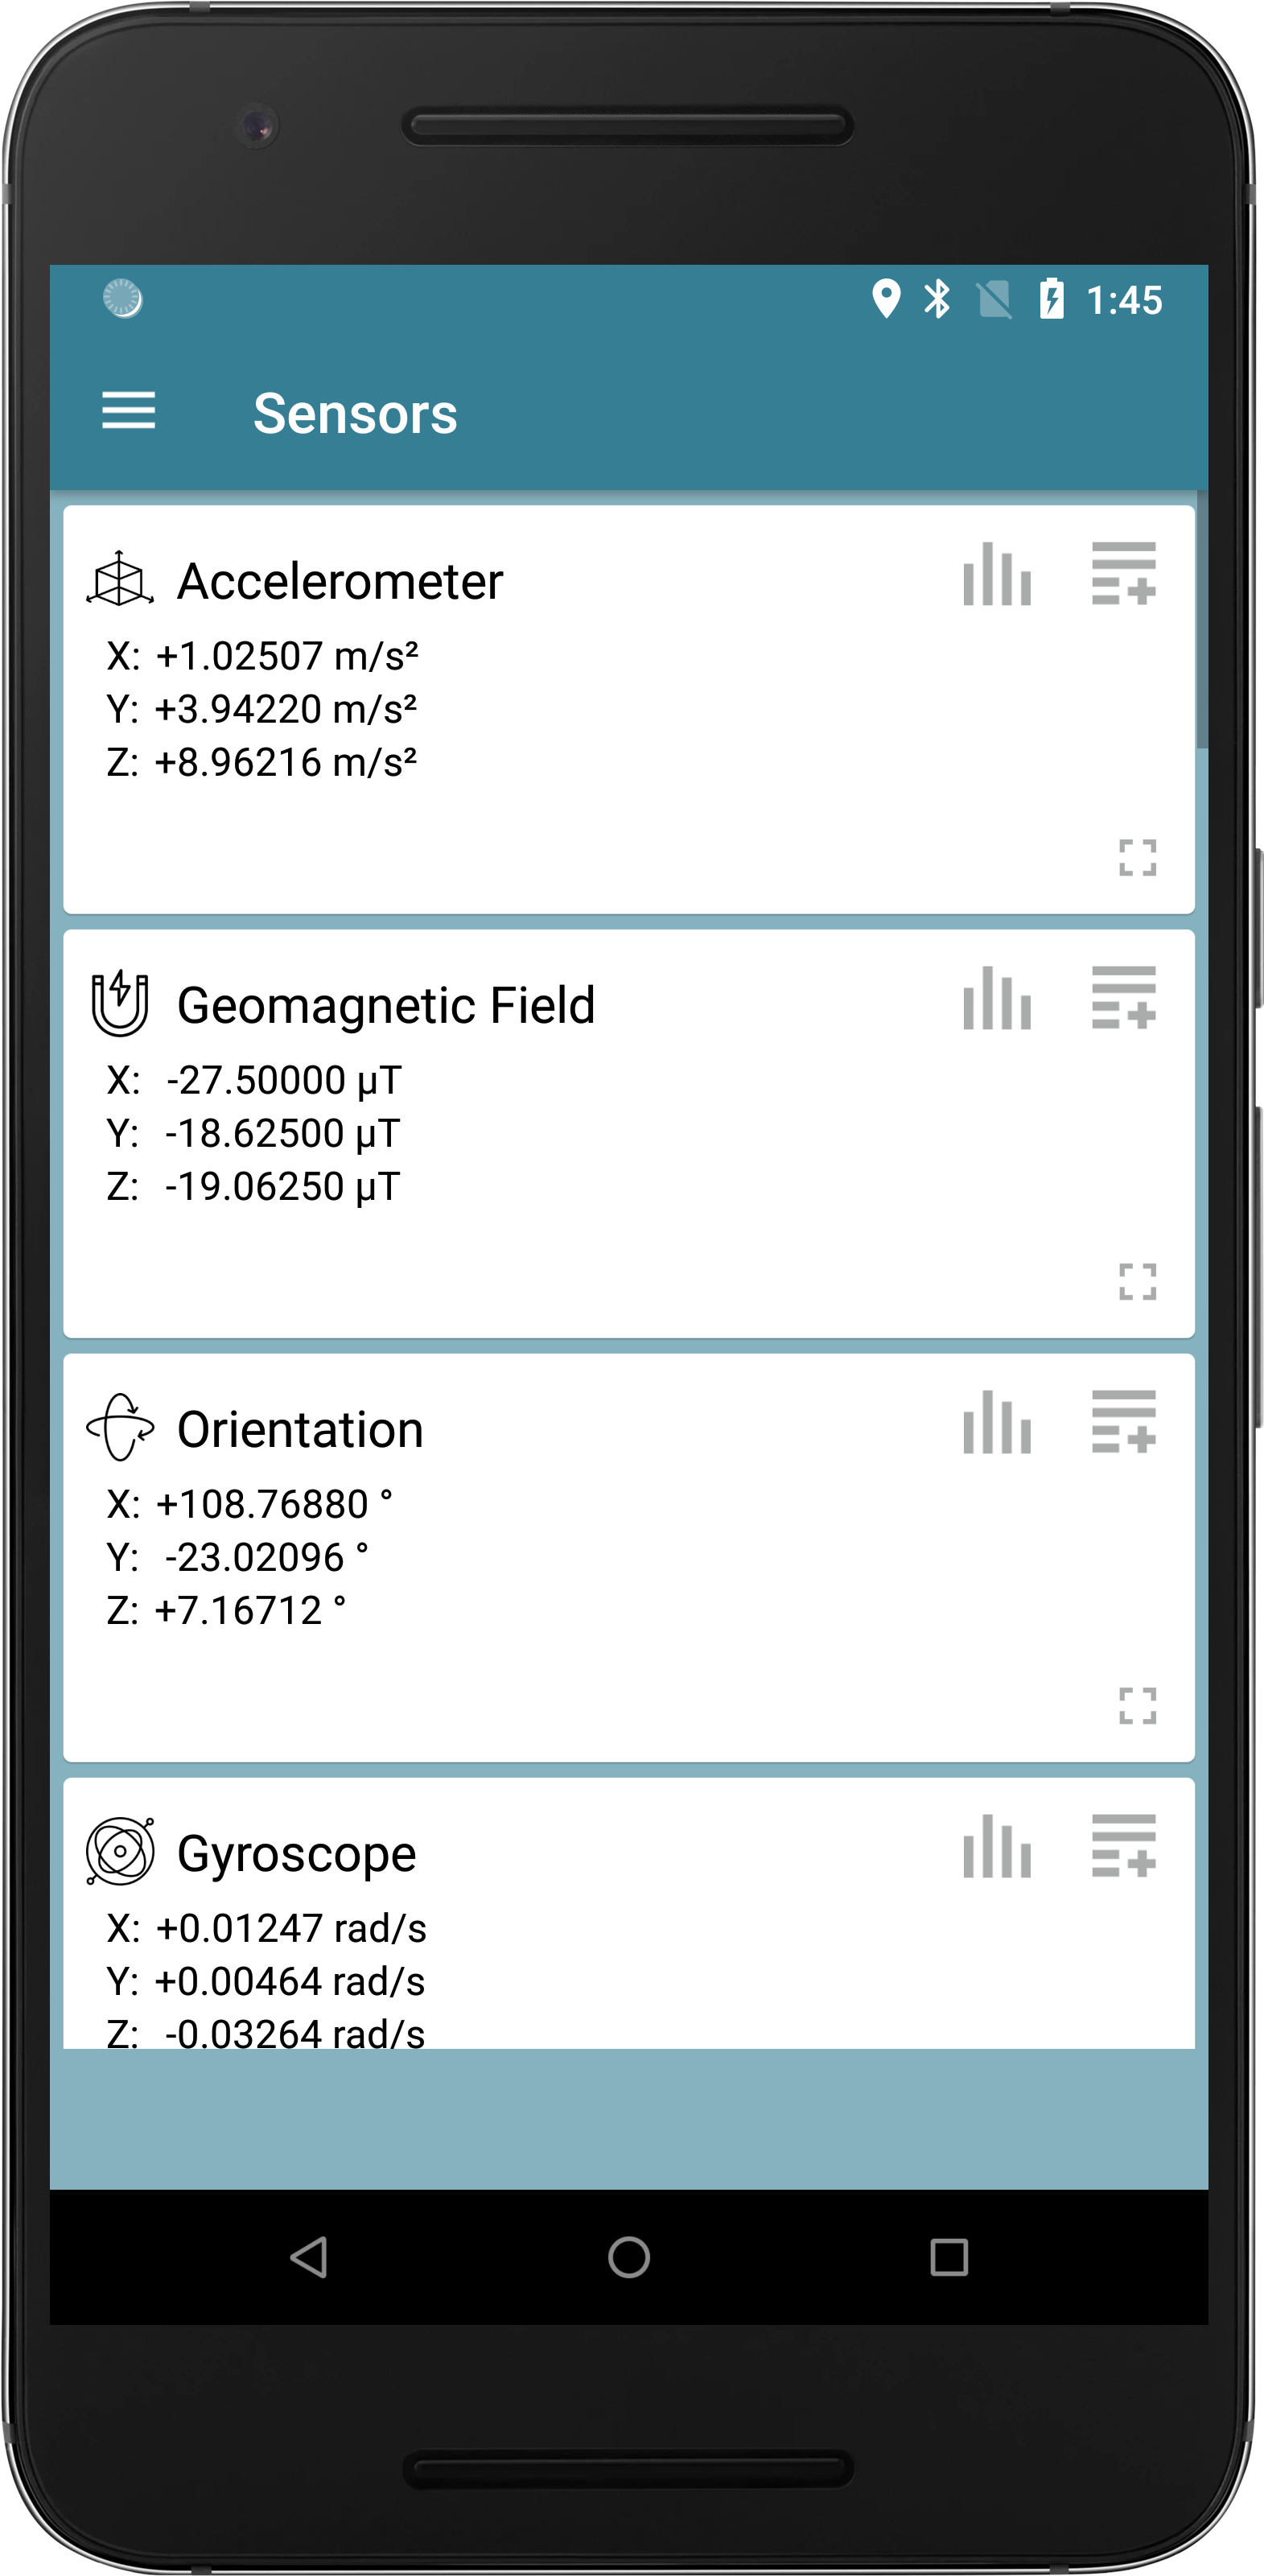
\includegraphics[width=1.4\textwidth]{sensors1}
		\end{minipage}
		\hspace{.60in}
		\begin{minipage}[t]{0.25\textwidth}
			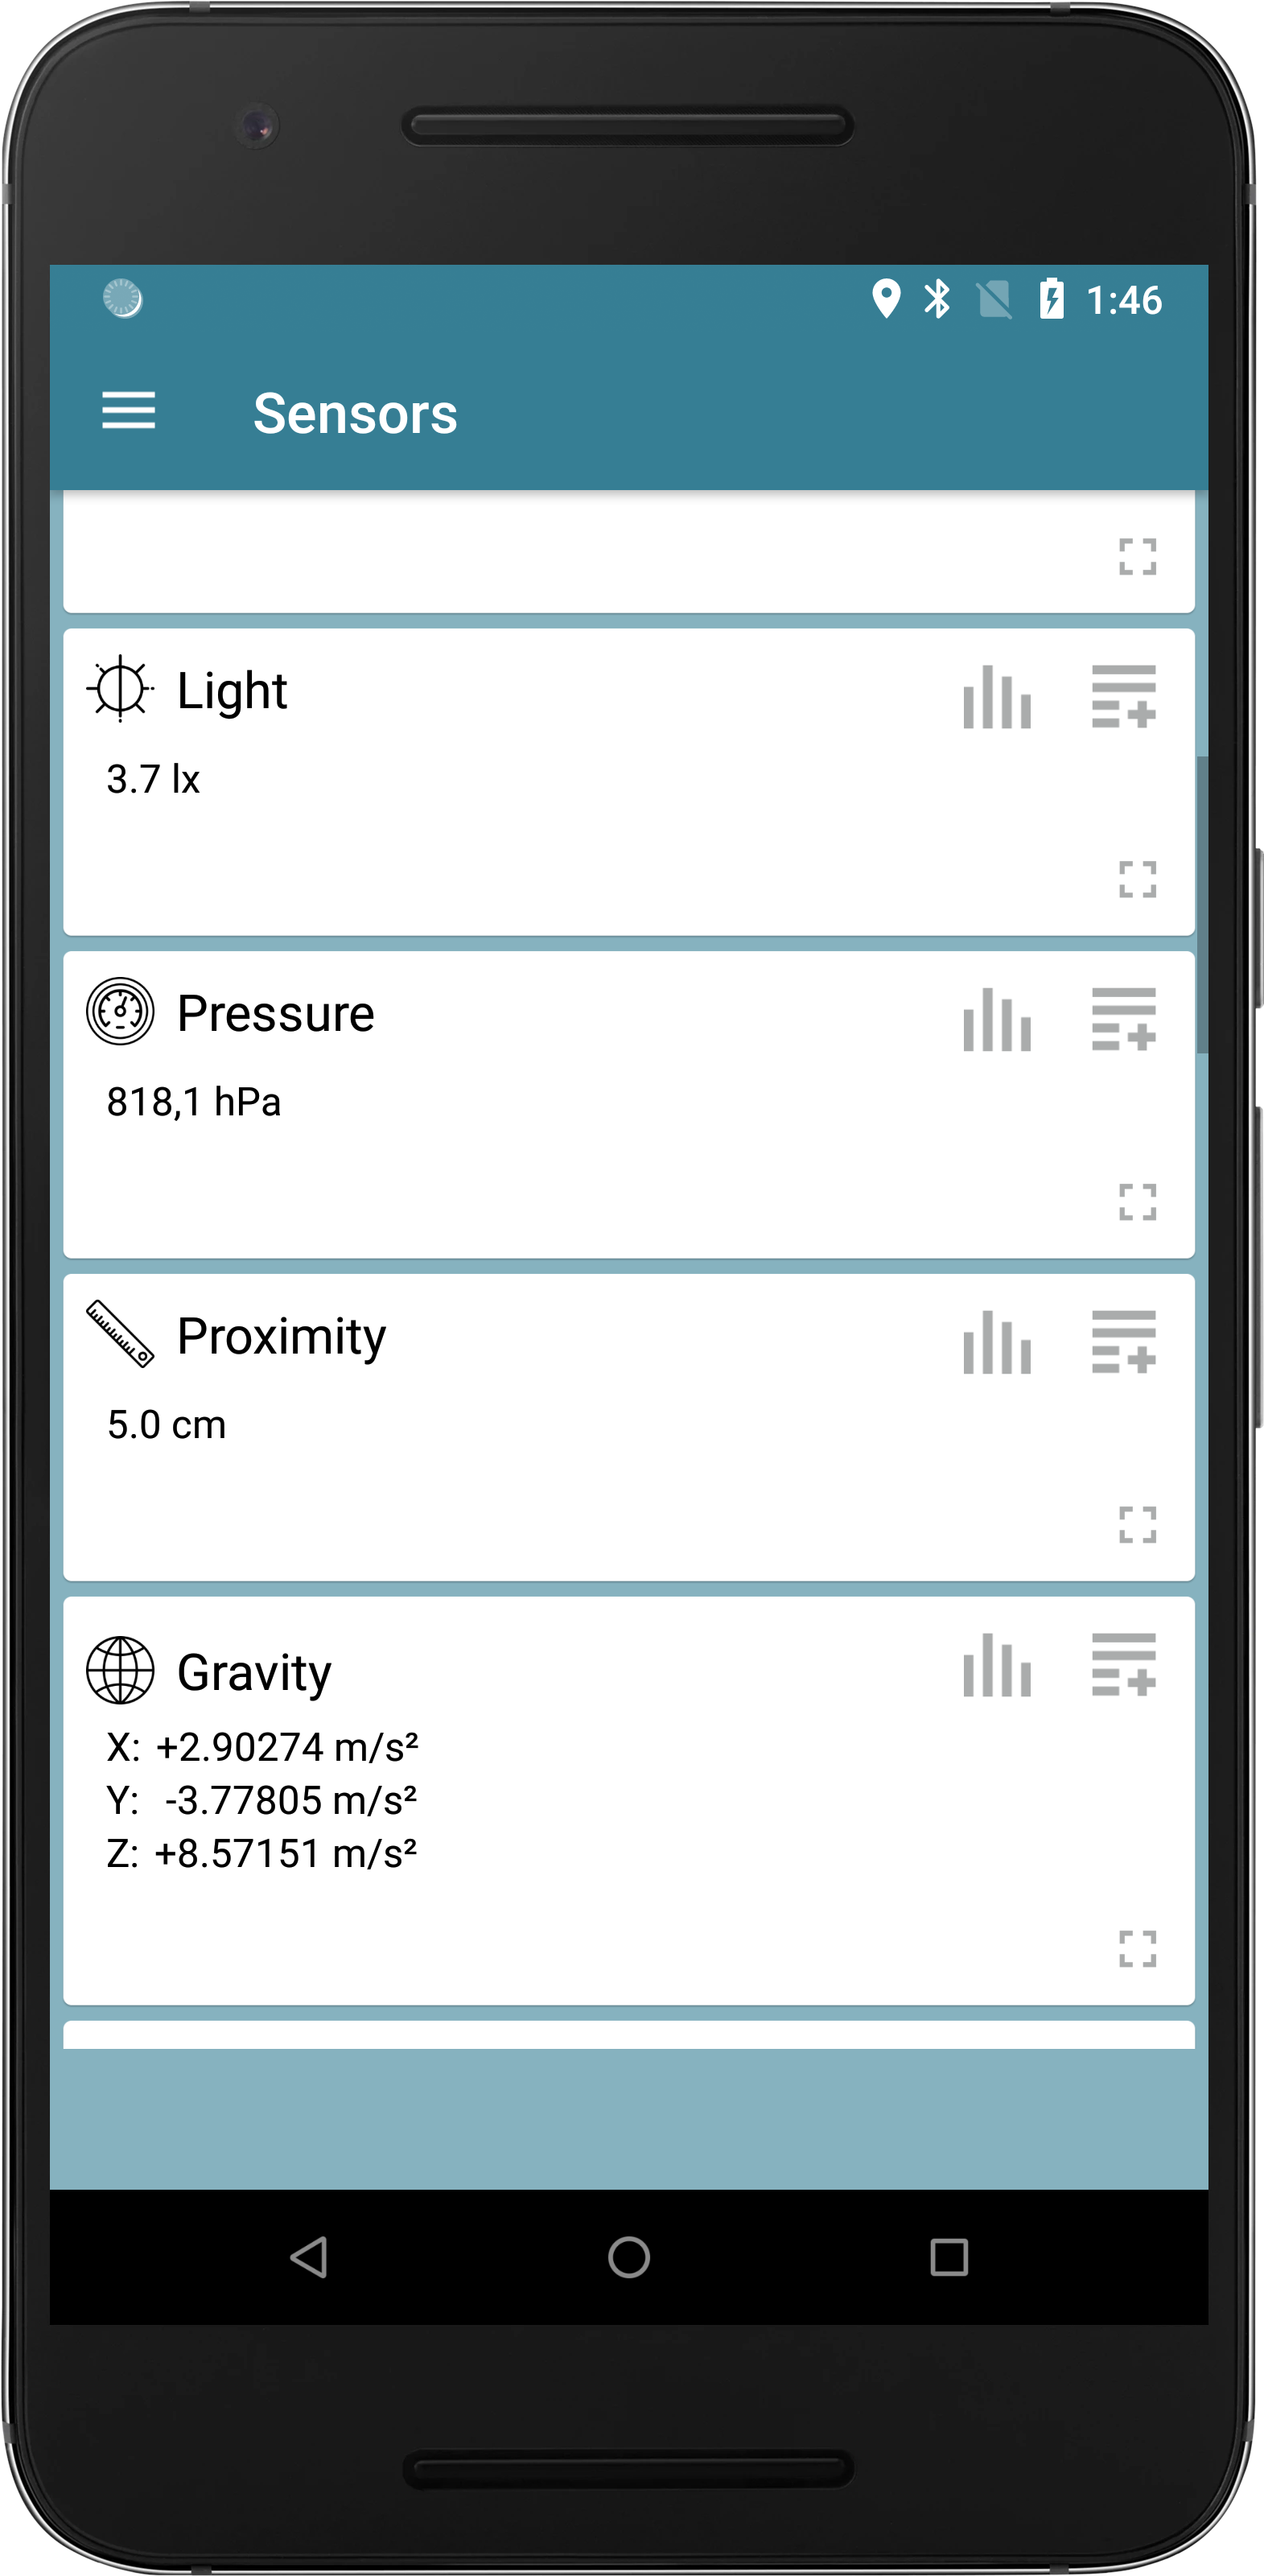
\includegraphics[width=1.4\textwidth]{sensors2}
		\end{minipage}
		\hspace{.60in}
		\begin{minipage}[t]{0.25\textwidth}
			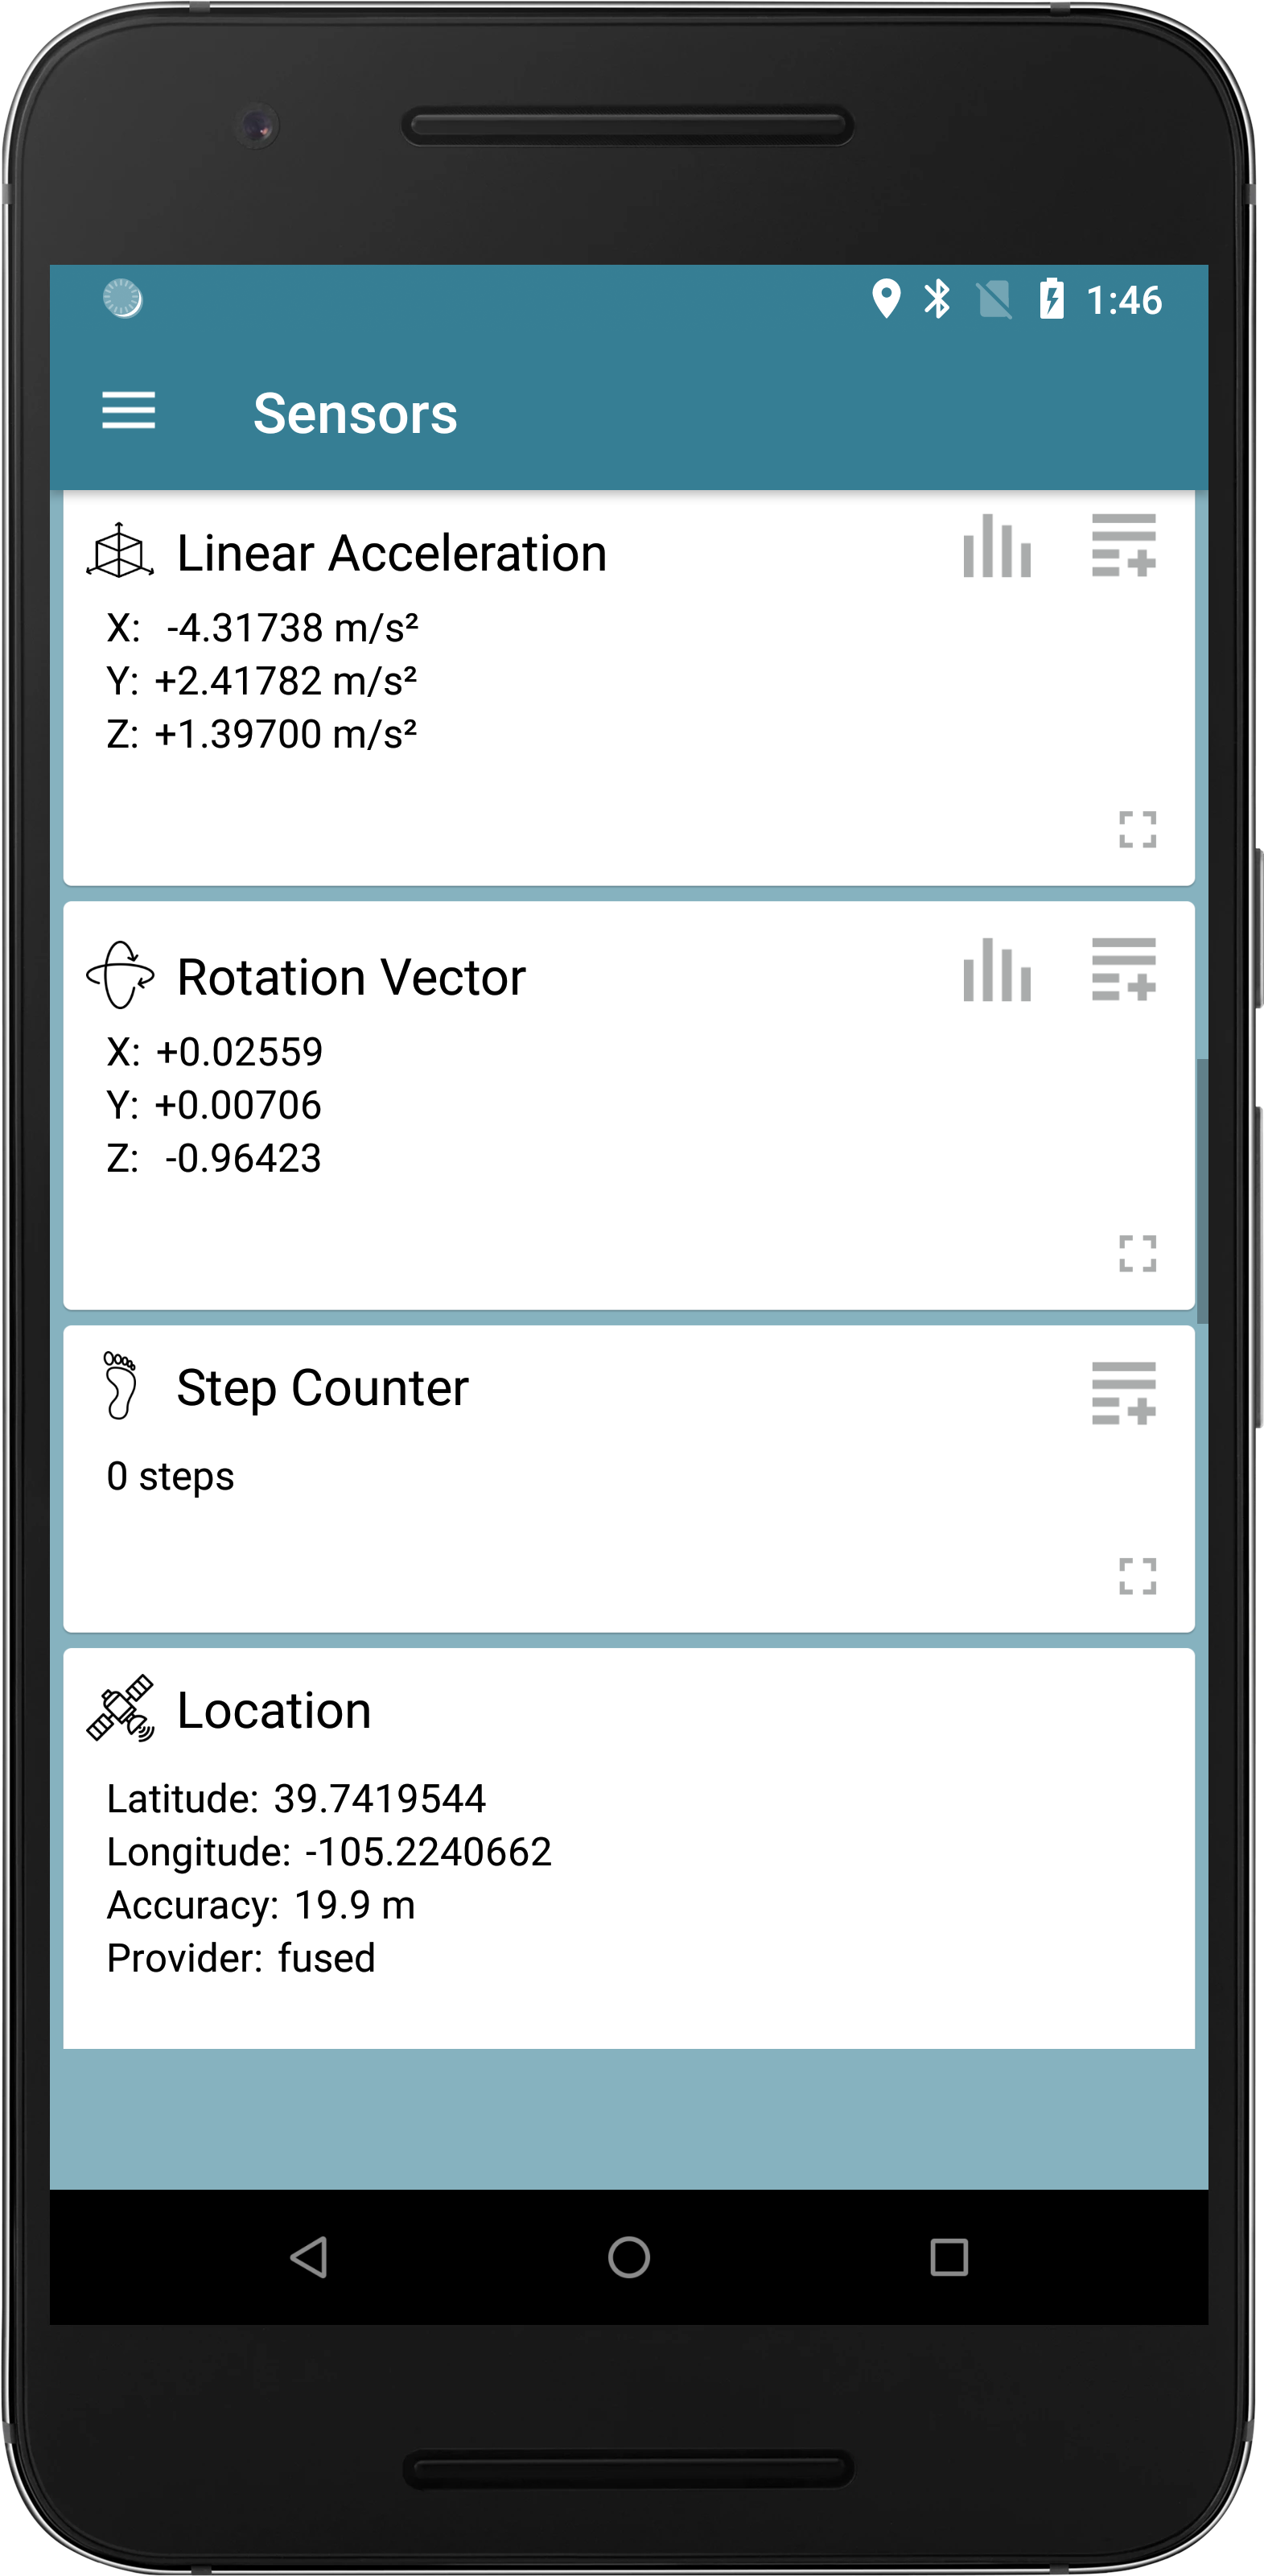
\includegraphics[width=1.4\textwidth]{sensors3}
		\end{minipage}  
		\hspace{.60in}
		\begin{minipage}[t]{0.25\textwidth}
			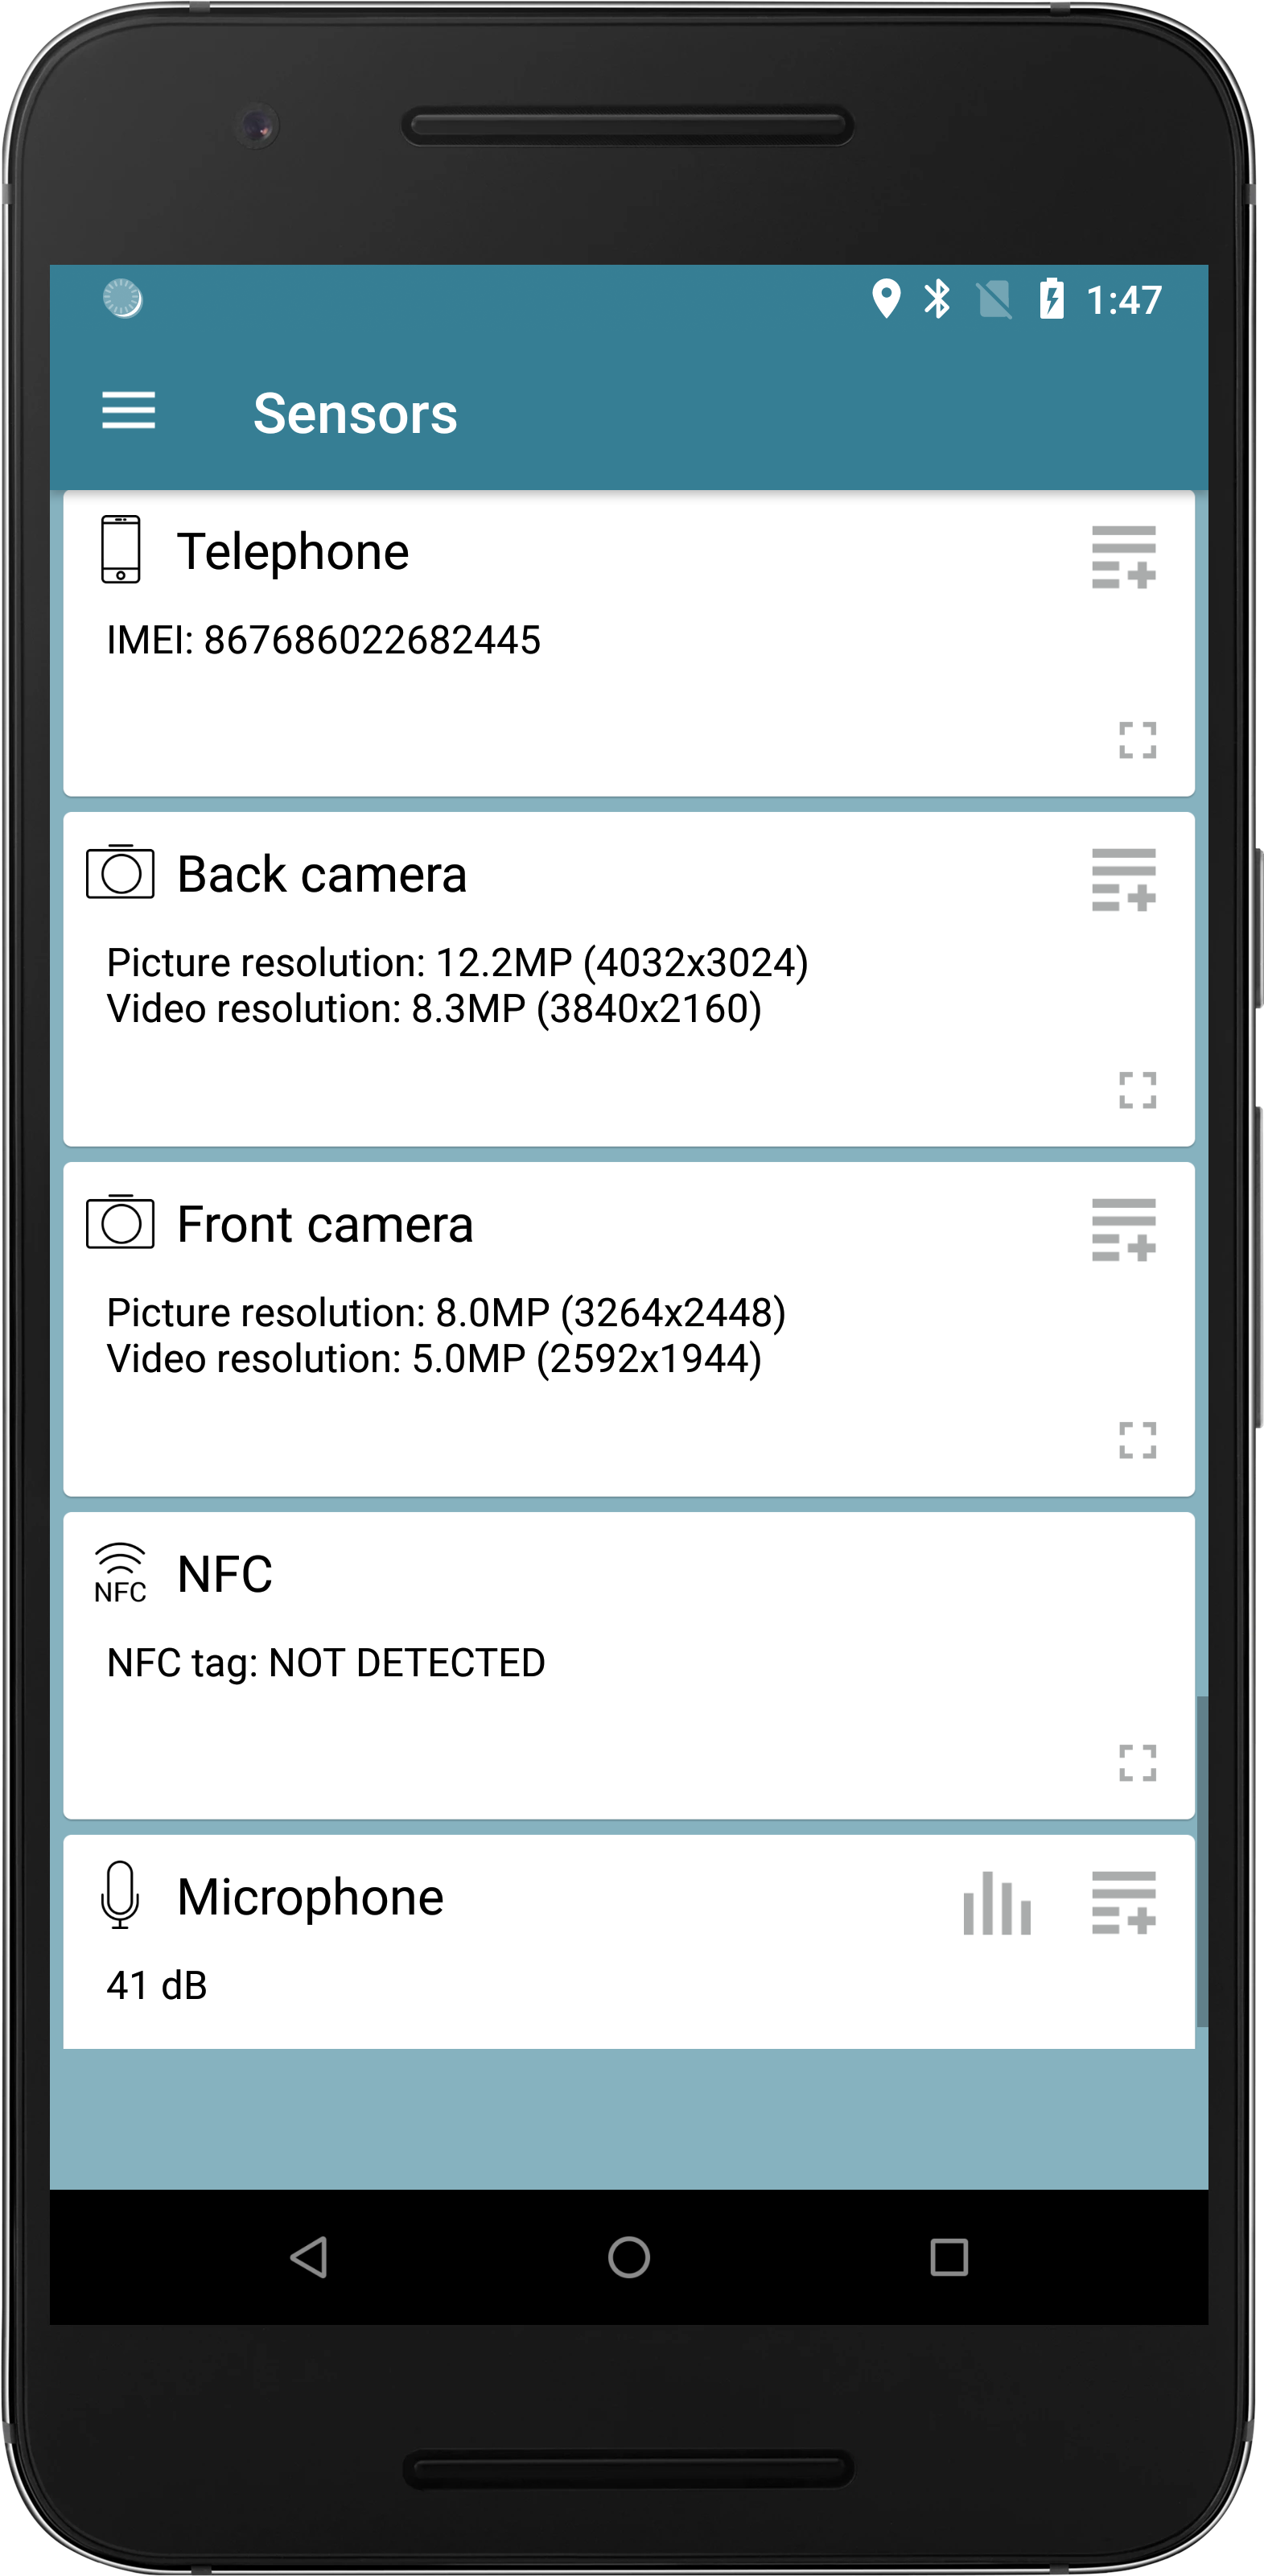
\includegraphics[width=1.4\textwidth]{sensors4}
		\end{minipage}  
		\caption{Real Readings of 18 Sensors on a Google Nexus 6P Device.}
		\label{fig:sensors}
	\end{figure*}
\end{landscape}

%TODO our approach

%========================================
%                            Chapter                            
%======================================== 
\chapter{{\spp}: Eavesdropping on Smartphone Speakers\protect \\ with Motion Sensors}

We introduce the \textit{{\attackName}} attack, which can turn smartphones into spy bugs. This attack is based on the fact that motion sensors (accelerometers and gyroscopes) can measure audio signals, though at a much lower sampling rate. This attack imposes a big threat to smartphone users since the phone's operating system grants applications permissions to motion sensors automatically. Compared to prior works, the {\attackName} attack focuses on the \textit{intra-device} scenario, where motion sensors eavesdrop on the same phone's built-in speakers. With compressed sensing theories and machine learning techniques, we implement the attack in an eavesdropping system called {\textit{\systemName}}, which is able to filch various critical information from smartphone users. Experiment results show that {\systemName} can learn user activity, speaker gender, speaker identity, and speech content with an average accuracy of 81\%, 93\%, 98\%, and up to 90\%, respectively. Apart from the good accuracy, the most significant contribution of this work is that the {\systemName} system is \textit{speaker-independent}. Unlike previous related works that need specific training data from the victim, {\systemName} is trained just once on public speech datasets and can filch critical information from brand new victims.
%========================================
%                            Section                             
%======================================== 	 
\section{Introduction}\label{sec:intro}
%Compared to traditional feature phones which are capable of voice calls and text messages,
%%
%smartphones bring many more applications including, but not limited to, email checking, web browsing, online shopping, game playing, music listening, video shooting, and GPS navigation.
%%
%%enable users to check their email, browse the web, post updates to social media sites, shop online, play games, listen to music,  shoot photos, and so on.
%%
%%can provide users with much more services such as email checking, web browsing, game playing, music listening, social chatting, video shooting, and so on. 
%%
%%
%With such extensive capabilities, smartphones have become ubiquitous and all-pervasive.
%%
%Indeed, the total number of smartphone users worldwide is over 3 billion this year - nearly 40\% of the human population, according to reports issued by several market-research firms~\cite{report2018newzoo,report2019forrester}. 

Smartphones have become one of the most popular devices in the last few years. According to Statista~\footnote{\url{https://www.statista.com/statistics/330695/number-of-smartphone-users-worldwide/}}, the current number of smartphone users in the world today is over 3 billion, and this means nearly 40\% of the world’s population owns a smartphone. 

In this thesis, however, we demonstrate how to turn smartphones to spy bugs which eavesdrop on everything played by smartphones' built-in speakers. Three billion smartphones? No, they are 3 billion spy-phones!
%
This dreadful attack, referred to as the \textit{{\attackName}} attack, is based on the fact that motion sensors (accelerometers and gyroscopes) can catch acoustic signals like a crude microphone. 
%
%
%What's worse, 
Thanks to smartphones' operating systems, accessing these sensors is effortless. 
%Smartphones' operating systems such as
For example,  Android
\footnote{\scriptsize iOS, Windows, and Blackberry OS have similar permission-based sensor management systems~\cite{sikder20176thsense}. In this work, we focus on Android.} 
automatically grants app permissions to motion sensors at installation time. In other words, any app installed in a smartphone can be a tool for attackers to eavesdrop covertly.
%iOS, Windows, and Blackberry OS have similar permission-based sensor management systems~\cite{sikder20176thsense}. In this work, we focus on Android.

%without notice. 
An example of attacking scenario is  illustrated in  Figure~\ref{fig:teaserpic}. A boy has a video call with his mom. He wants to buy a book online and he needs her mom’s credit information to place an order. Her mom’s voice is played by the loudspeaker on the smartphone and affects the readings by motion sensors. The attacker has access to the motion data and therefore can infer the credit card information.  
%

\begin{figure}
	\centering
	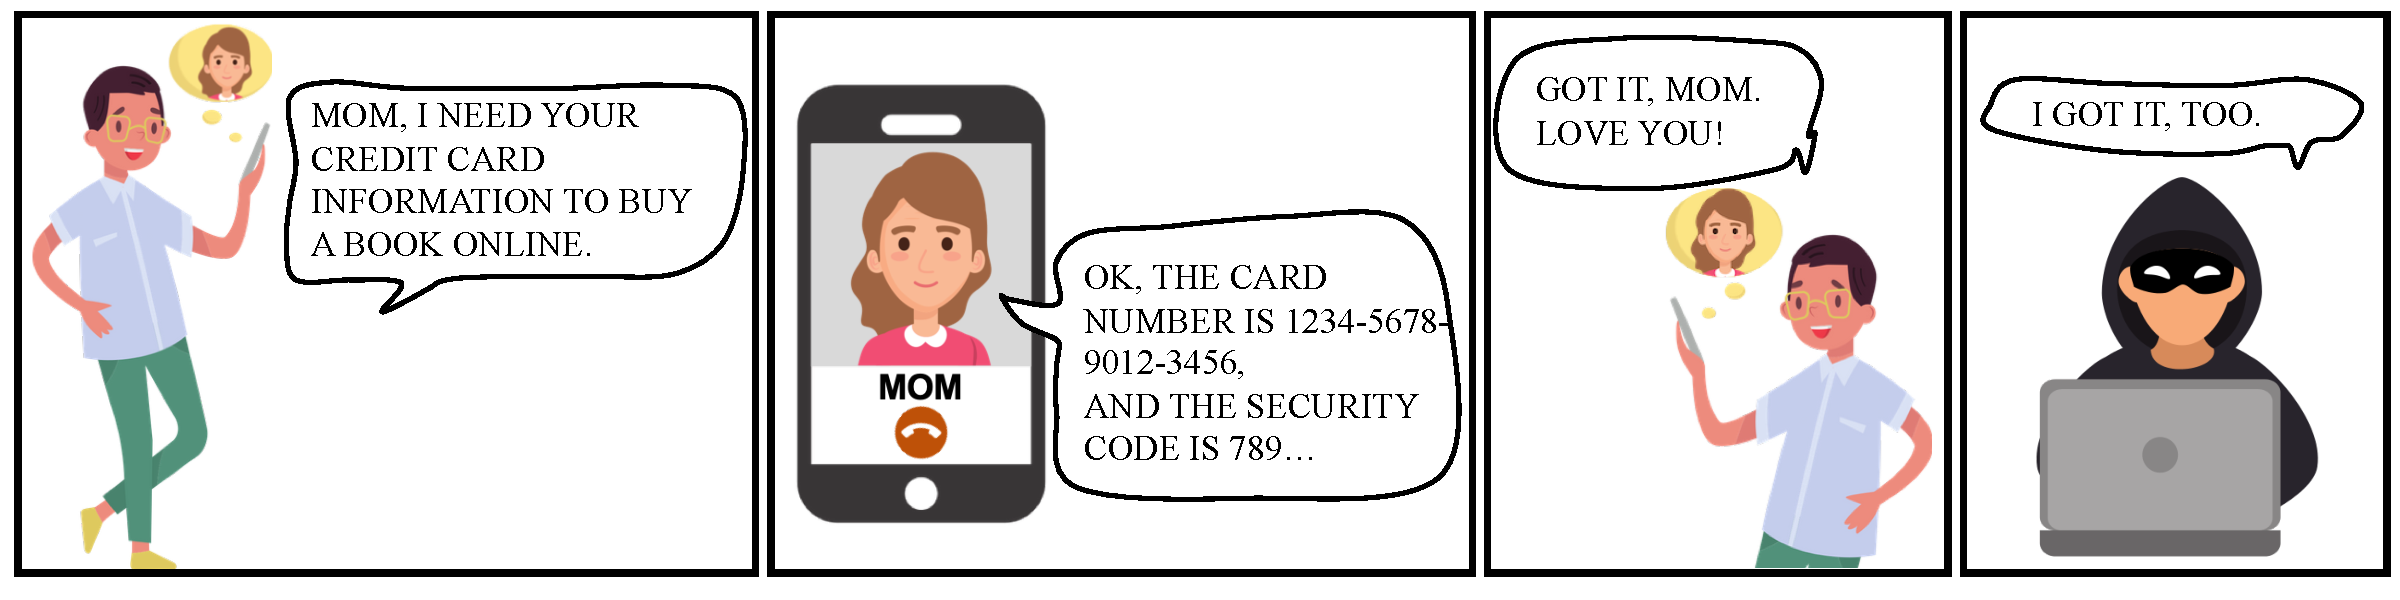
\includegraphics[width=\linewidth]{Figures/SpyPhone/teaserpic}
	\caption[Example of an Attacking Scenario.]{Example of an Attacking Scenario by {\spp}. A seemingly harmless application (a weather app for example) is installed on the phone, and it keeps accessing the motion sensors in background. Attackers can infer acoustic signals from the under-sampled motion data. }
	\label{fig:teaserpic}
\end{figure}



In fact, there have been some recent studies about the side-channel leakage from acoustic signals to smartphones' motion sensor readings. Michalevsky et al.~\cite{michalevsky2014gyrophone} proposed \textit{Gyrophone} in 2014. To the best of our knowledge, they are the first to use smartphone gyroscopes as low-frequency microphones to listen to loudspeakers. Gyrophone can differentiate 11 digits with 65\% accuracy based on a 10 people dataset.
%Michalevsky et al.~\cite{michalevsky2014gyrophone} are the first to use smartphone gyroscopes as low-frequency microphones. 
%However, they only tested their work on a small dataset (10 people) and achieved a digit recognition rate of 65\%. 
One year later, Zhang et al.~\cite{zhang2015accelword} proposed \textit{AccelWord}, which utilizes accelerometers to classify hotwords such as ``Okay Google'' or ``Hi Galaxy'' over other short phrases with 85\% accuracy. AccelWord is also tested over 10 people.
%However, their work lacks credibility due to limited dataset (10 people) and small classifying number (3 classes). 

However, techniques proposed in neither Gyrophone nor AccelWord can be used to perform a {\attackName} attack. Because these systems are built upon a \textit{speaker-dependent} model, i.e. training dataset are labeled data from the target speakers. In the {\attackName} attack, attackers will not get \textit{labeled} motion data from the victim  ------ the attack system should be \textit{speaker-independent}.

In 2018, Anald and Saxena~\cite{anand2018speechless} reproduced the aforementioned works and overturned their conclusions. They argued that smartphone motion sensors can not be affected by the speech signals transmitted through the air, no matter the sound source is a loudspeaker or a live person. They reported that only when the speakers and the motion sensors sharing a surface,  the \textit{conductive vibrations} will affect motion sensors' readings. Except for this ``Loudspeaker-Same-Surface'' scenario, they studied 5 other  scenarios
\footnote{\scriptsize``Loudspeaker-Different-Surface'', ``Laptop-Same-Surface'', `` Phone-Different-Surface'', 		``Human-Normal'', and ``Human-Loud''.}  
%(``Loudspeaker-Different-Surface'', ``Laptop-Same-Surface'', `` Phone-Different-Surface'', 		``Human-Normal'', and ``Human-Loud'')
and concluded that smartphone motion sensors only pose a limited threat to speech privacy.
% since conductive vibrations are ``possibly less common''.
%the impact of speech signals is very limited on motion sensors. 
%
However, they missed one important scenario,  the \textit{intra-device} scenario, where the speakers and motion sensors are inside the same smartphone. In 2019, they investigated this remaining scenario in an arXiv paper~\cite{anand2019spearphone} and their SpearPhone system recognize 11 digits with an accuracy of 71\%.  However, their technique is still speaker-dependent, which means the original speech data of the target speaker must be collected ahead of time. Such requirement is very hard to be fulfilled in practice.

In this thesis, we studied the side-channel attack in the intra-device scenario. This \textit{{\attackName}} attack, as we refer to it, is speaker-independent.


%\begin{figure}[!h]
%\centering
%\subfloat[][]{.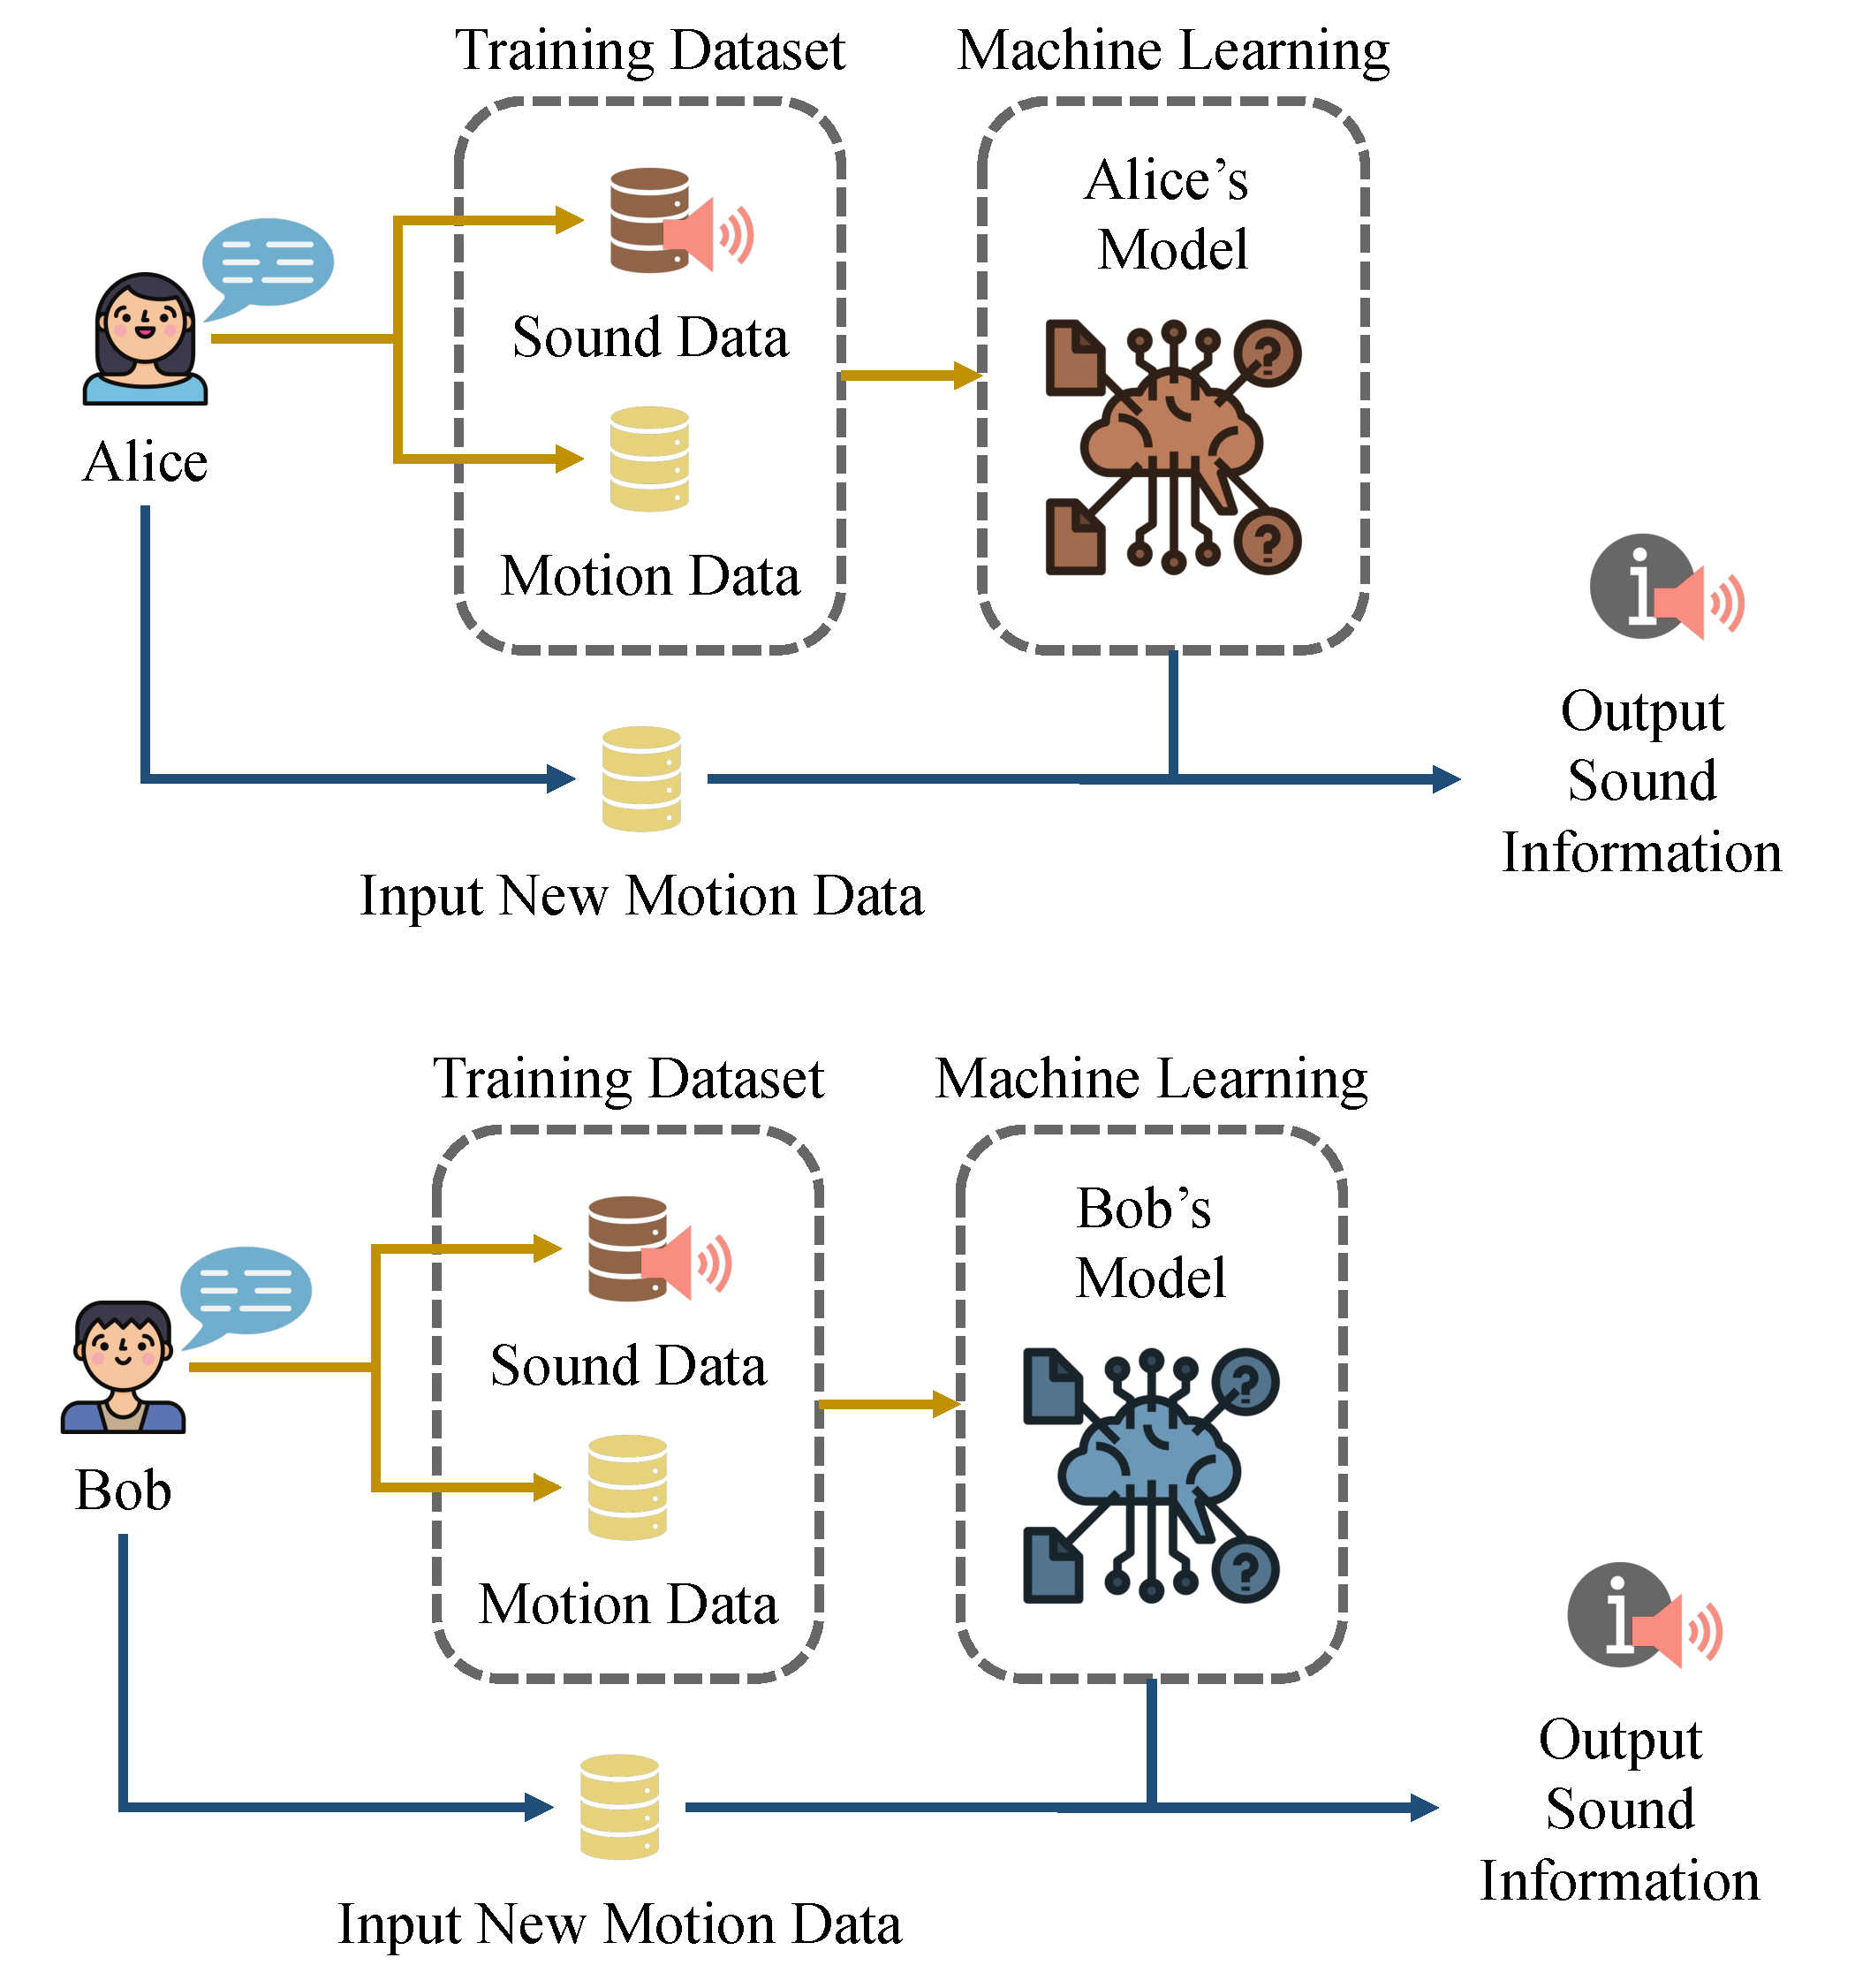
\includegraphics[width=.9\linewidth]{speakerDependent}
%	\vspace{-.05in}
%	\caption{Mathematical model of a typical compressed sensing system. }%
%\qquad
%\subfloat[][]{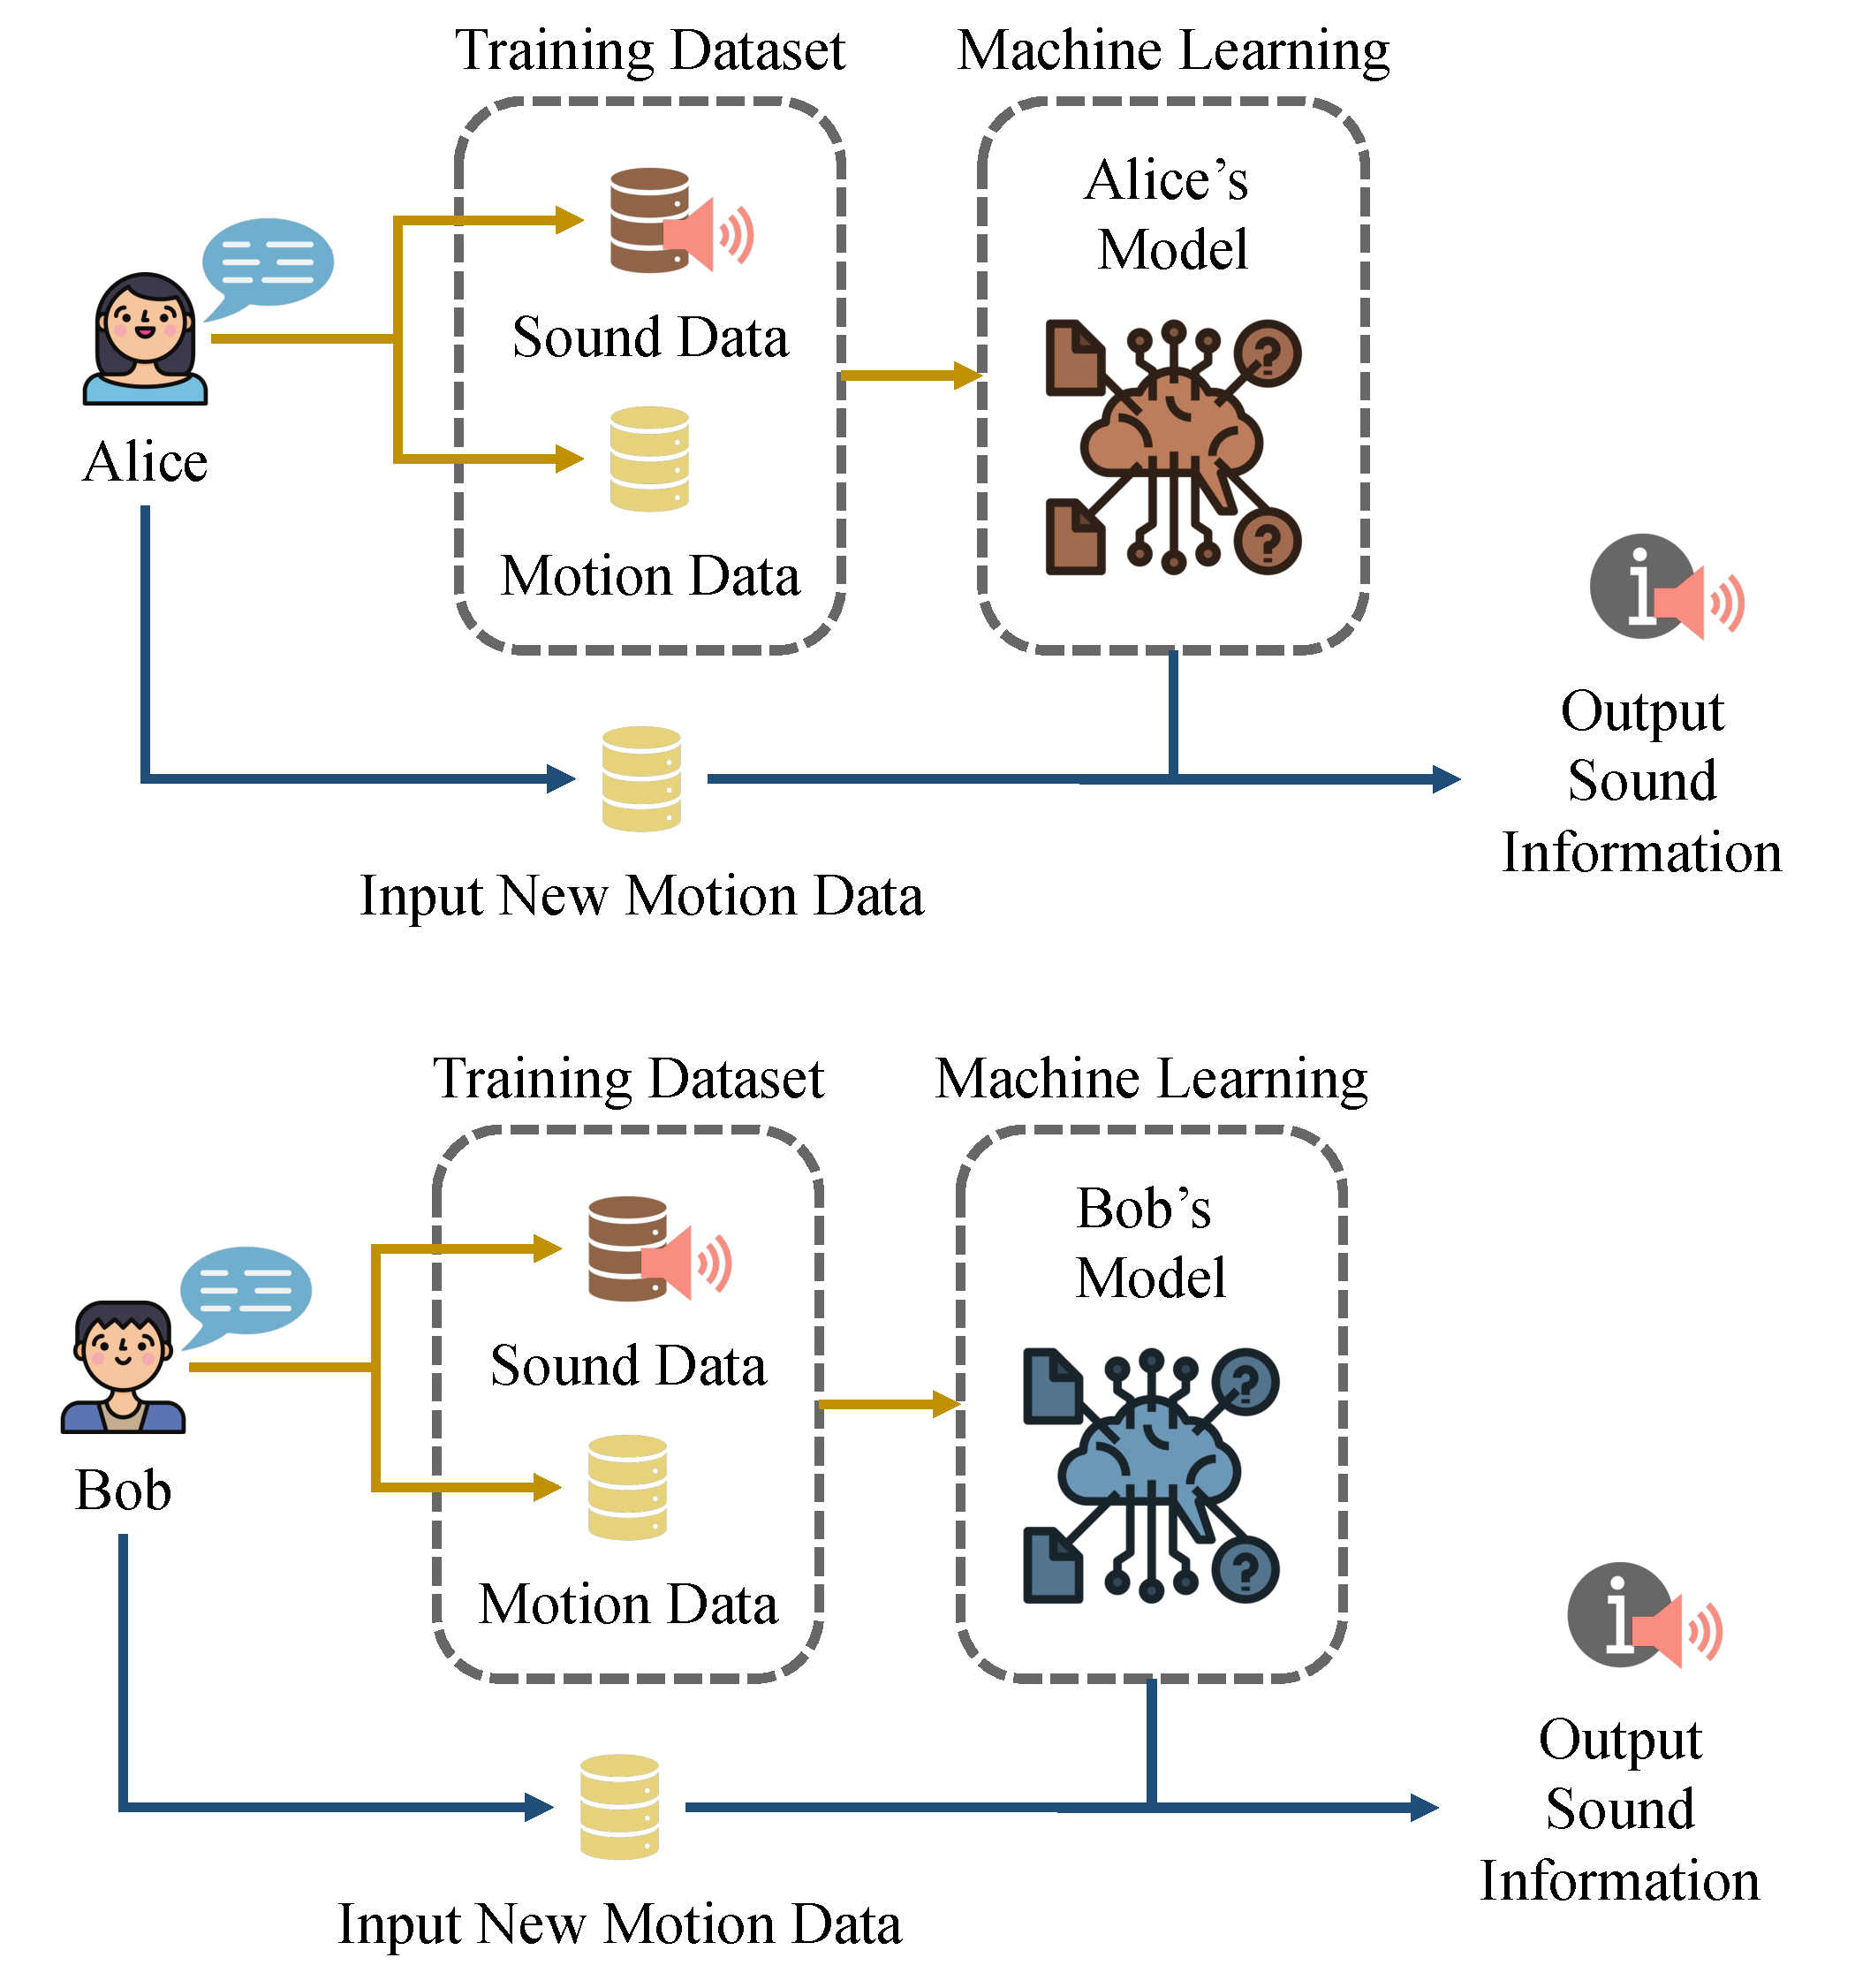
\includegraphics[width=.9\linewidth]{speakerDependent}
%	\vspace{-.05in}
%	\caption{Mathematical model of a typical compressed sensing system. }
%\caption{Here are the first two figures of a continued figure.}% \label{fig:cont}
%\end{figure}
% Attackers do not need to get the target victim's speech data and they can still filch critical information from the 


% https://arxiv.org/abs/1907.05972
%The side-channel attack in this scenario, or the \textit{{\attackName}} attack as we refer to it, is the focus of this paper. We agree with Anald and Saxena on that motion sensors are more sensitive to conductive vibrations than aerial vibrations, but we show motion sensors can leak various critical information and pose a big threat to smartphone users' security and privacy. 

% accelerometer when the laptop and the motion sensor shared a surface.
%
%direct acoustic aerial vibrations 
%
%
%aerial vibrations. We also report that in the presence of live human speech, we did not 
%
% the recorded effect on the sensor readings is possibly from conductive vibrations through the shared surface instead of direct acoustic vibrations due to speech as perceived in previous work. S
%
%
%. They stated that smartphone speakers were not found to be powerful enough to invoke a response in the motion sensors \textit{through aerial vibrations}. They also reported that in the presence of live human speech, they did not notice any effect on the motion sensor readings.

%Different research groups draw conflicting conclusions. So who is right? We have done similar experiments and the findings are similar to that of Anald and Saxena. Unless a person speaks really loudly (shouting, usually 10 dB higher than normal speech),  or use commercial loudspeakers (not MEMS speakers inside smartphones) on the same surface with the smartphone, it is hard to identify the sounding period based on motion sensors. Moreover, the distance between the sound source and the smartphones must be short (less than 30 cm). 

%However, Anald and Saxena's work is not perfect. Although they studied this side-channel leakage in 6 different scenarios and showed the threats only have significant impacts in the ``Loudspeaker-Same-Surface'' scenario, they missed one important scenario, the \textit{intra-device} case, where the speakers and motion sensors are inside the same device. This scenario, or the \textit{{\attackName}} attack as we refer to it, is the focus of our research.

%
%It is also worth mentioning that prior works such as  Gyrophone~\cite{michalevsky2014gyrophone} and AccelWord~\cite{zhang2015accelword} can only achieve the claimed accuracy in the speaker-dependent setting. But a speaker-dependent setting requires the system to get specific training data from the target user. Such condition may not be satisfied in real attacking scenarios. When Gyrophone use an speaker-independent setting to identify digits, the maximum accuracy  is only 26\%.

\begin{table}[h]
	\caption{Maximum Sampling Rate of Smartphone Sensors}
	%	\footnote{Some part of the data is from~\cite{matyunin2018zero}, others are tested }
	\label{tab:sample}
	\centering
	
	%	\resizebox{\columnwidth}{!}{
	\begin{tabular}{cccc} %{lp{2cm}p{2cm}}
		\toprule		
		Device & \makecell{Release \\Year} & \makecell{Speakers' \\ Sampling Rate} & \makecell{Motion Sensors' \\ Sampling Rate
			\footnotemark} \\
		\midrule
		Samsung Galaxy S8 & 2017 & 192,000 Hz & 500 Hz\\
		Samsung Galaxy S7 & 2016 & 192,000 Hz & 500 Hz\\		
		Google Nexus 6P & 2015 & 48,000 Hz & 400 Hz\\
		LG Nexus 4 & 2012 & 48,000 Hz& 200 Hz\\
		\bottomrule
	\end{tabular}
	%}
\end{table}



\footnotetext{\scriptsize Data is partially from~\cite{matyunin2018zero} and partially by calling the \texttt{getMinDelay()} function of \texttt{android.hardware.Sensor} class.}

%To sum up, we show how to design an eavesdropping system that measures the conductive vibrations from smartphones' built-in MEMS speakers to MEMS accelerometers and gyroscopes. The main challenges in performing such an attack are:
%In this paper, we design an eavesdropping system named \textit{{\systemName}} which implements the speaker-independent {\attackName} attack. 
The main challenges in designing such a system are:
 \begin{itemize}
 	\item  The motion sensor readings are affected by at least four types of signal sources: sensor intrinsic errors, movement of the smartphone, acoustic vibrations from built-in speakers, acoustic vibrations from the air or other sound sources. An efficient filter is needed since only the acoustic vibrations from built-in speakers is the signal of interest.
 	
 	\item As shown in Table~\ref{tab:sample}, compared to the sampling rate of smartphones' built-in speakers which can reach 192 kHz, the sampling rate of motion sensors is 200-500 Hz. With such low frequency, human ears are no longer able to retrieve the original information, neither do state-of-the-art speech recognition systems~\cite{michalevsky2014gyrophone}.
 	
 	\item As illustrated in Figure~\ref{fig:depend}, the system should be speaker-independent. Prior works such as  Gyrophone~\cite{michalevsky2014gyrophone} and AccelWord~\cite{zhang2015accelword} can only achieve the claimed accuracy (65\% for 11 classes and 85\% for 3 classes) in the speaker-dependent setting. When Gyrophone uses an speaker-independent setting to identify digits, the
 	accuracy is only 26\%. This indicates that building a speaker-independent system is much more challenging than a speaker-dependent one.
 	
% 	harder than a speaker-dependent system.
% 	%TODO.
% 	In addition
% 	However, the speaker-dependent setting requires the system to get specific training data from the target user. Such condition may not be satisfied in real attacking scenarios. 
 \end{itemize}

%
%44.1 kHZ, 48kHz, 96kHz, or even 192kHz\footnote{Example sampling rate as shown in \url{https://developer.android.com/ndk/guides/audio/sampling-audio}.}, 
%The impact of the studied threat under the designed scenarios therefore limits itself to only specific settings. F
%
%
%information leakage from physical properties, or side-channels


%
%Consequences:
%know the gender
%know the number
%know your activity
%
%Contributions
%

%How we conquer the challenges?

%Although reconstructing original sound signals from motion data is impossible, partial information can be learned by {\attackName} attackers. Such information includes user activity, speaker gender/identity, and speech content (as elaborated in Section~\ref{sec:threat}). 

%\footnote{We refer the attack as the {\attackName} attack, and the system designed to perform such an attack as the {\systemName} system.}



Despite these challenges, the {\systemName} system is able to learn variety of critical information from smartphone users, such as user activity, speaker gender/identity, and speech content (as elaborated in Section~\ref{sec:threat}). 
These achievements are largely credited to the compressed sensing theories which allow recovering certain signals from fewer samples than required in Nyquist paradigm (as elaborated in Section~\ref{sec:background}); and the machine learning techniques named Bi-directional Long Short-Term Memory (Bi-LSTM) network, which is a special variant of recurrent neural networks. 




\begin{landscape}
	\begin{figure*}[h]%
		\centering
		\begin{minipage}[c]{.45\linewidth}
%			\begin{subfigure}[t]{1.3\textwidth}
				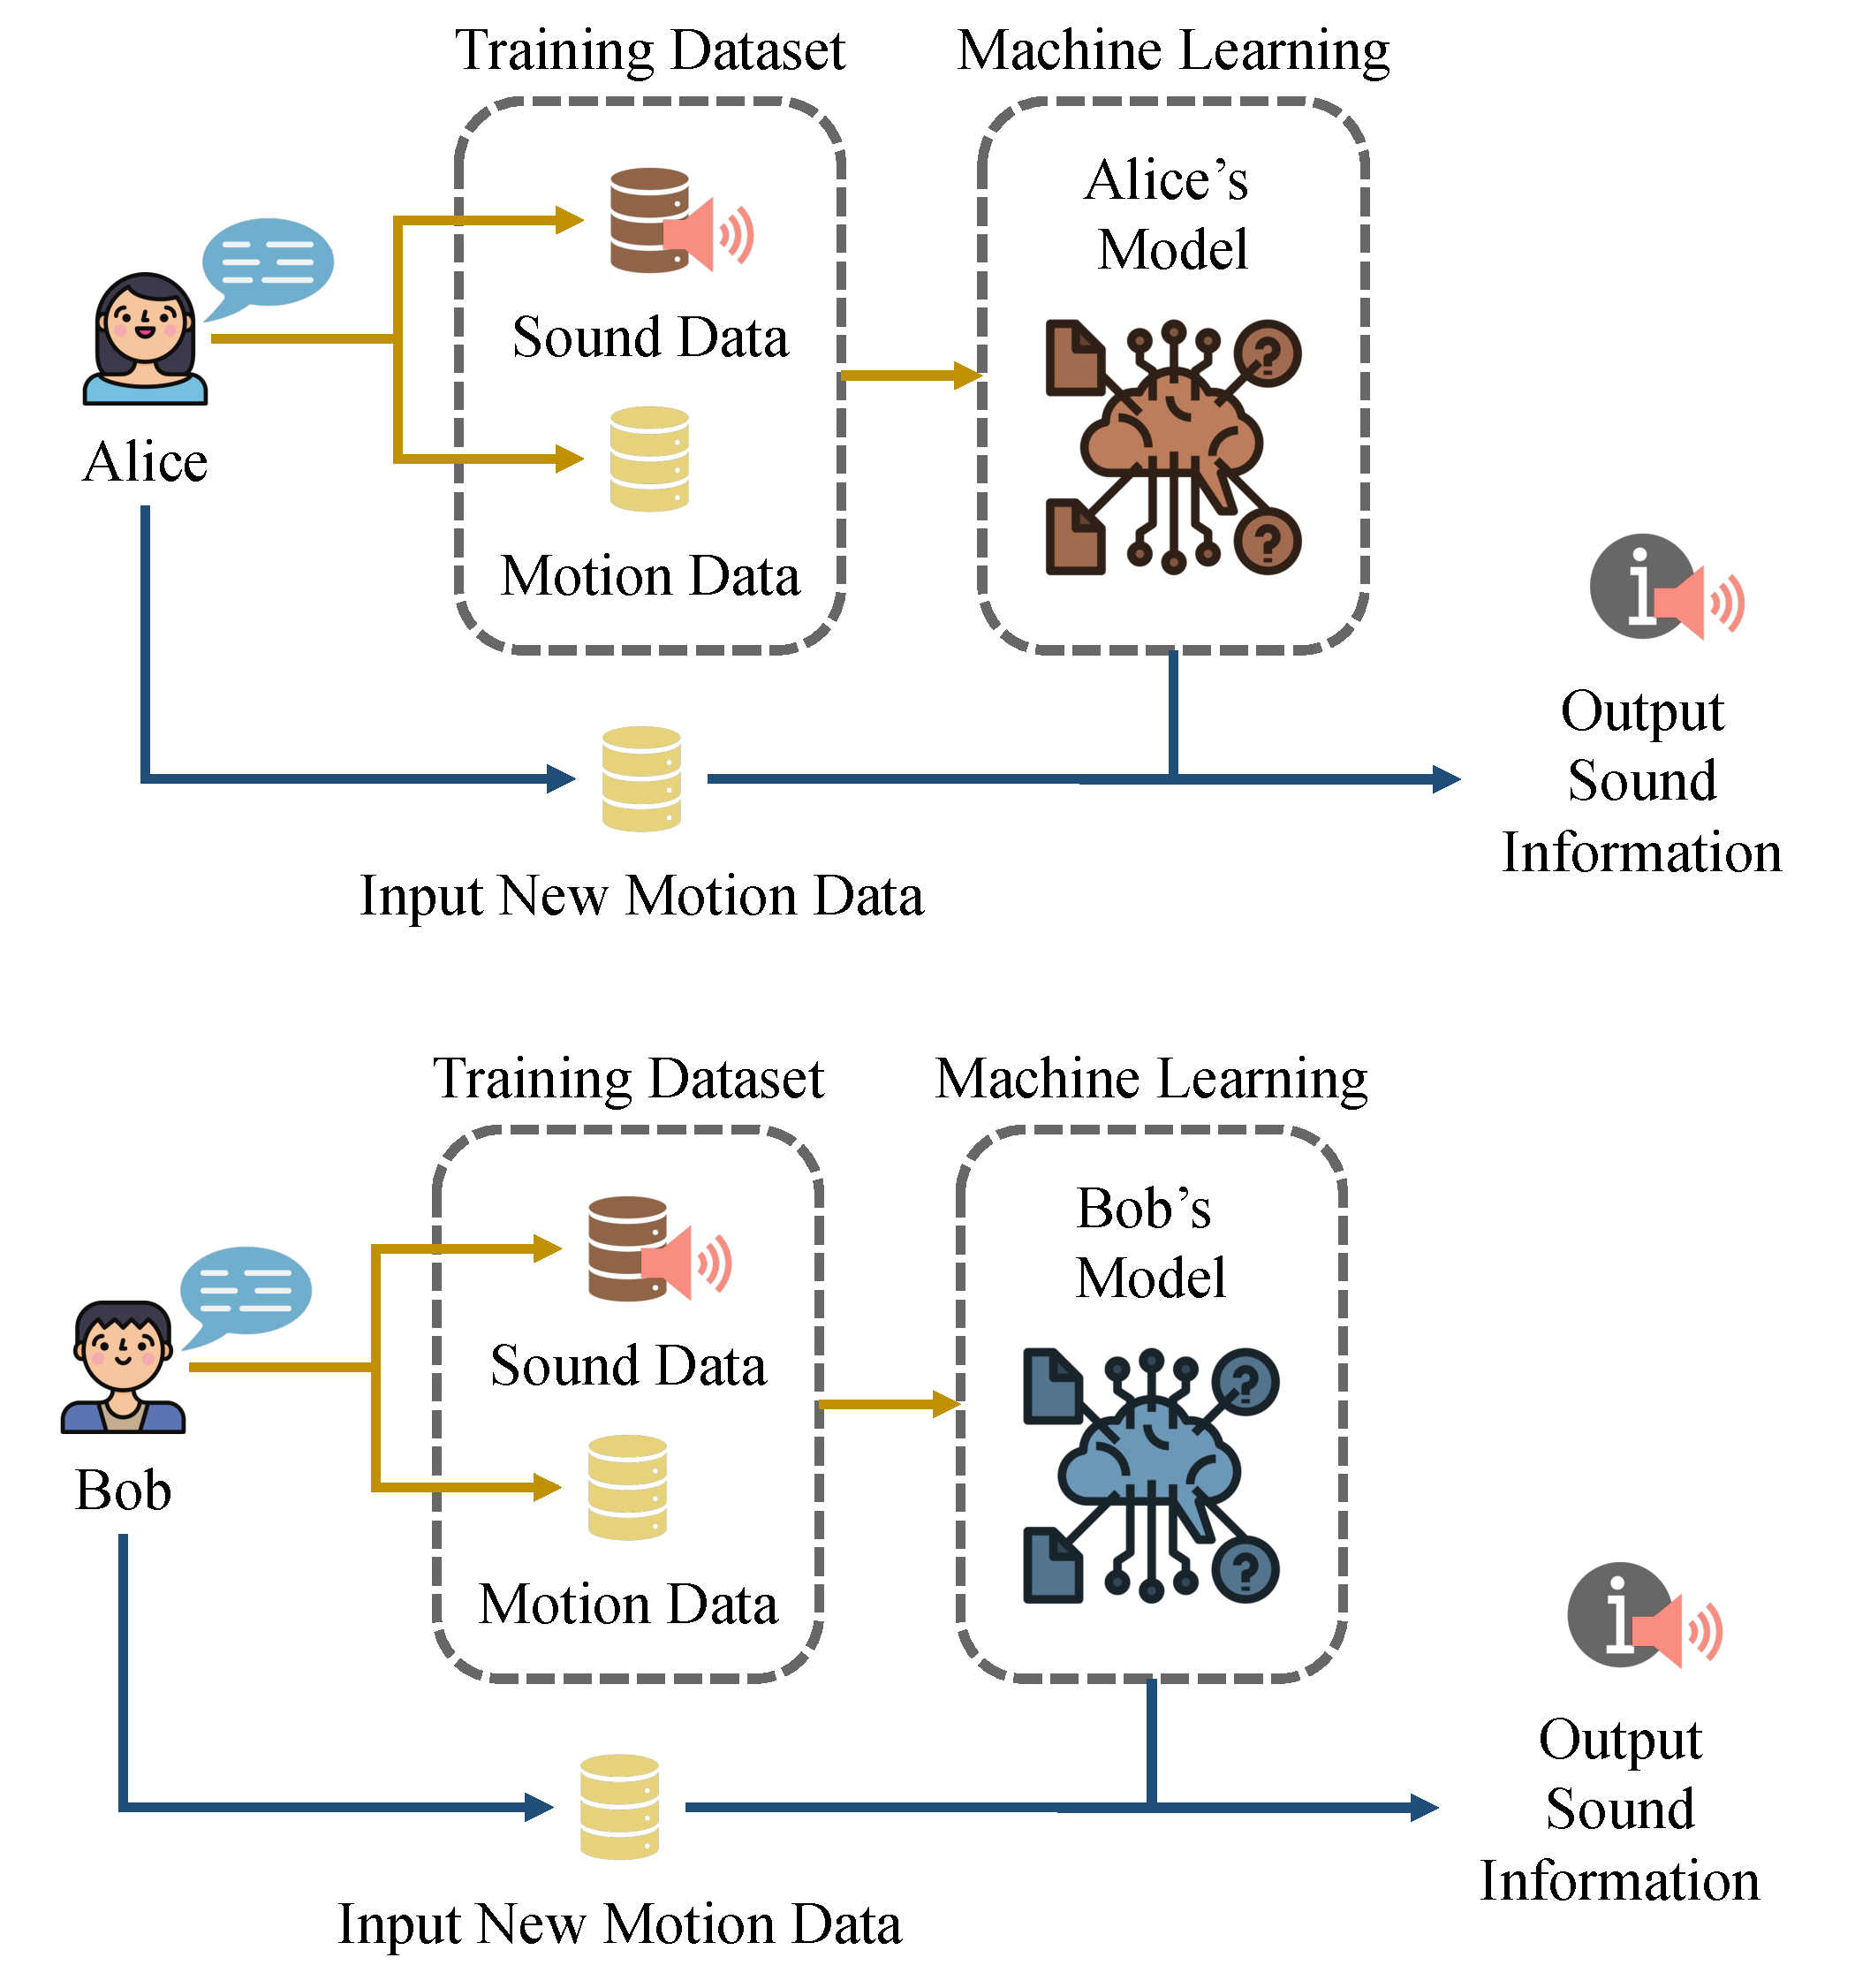
\includegraphics[width=\textwidth]{speakerDependent}
				\subcaption{Speaker-Dependent: target speaker's training data is required. After machine learning procedures, the trained models  for different speakers are different.}
%			\end{subfigure}
		\end{minipage}
		\begin{minipage}[t]{.05\textwidth}
			\qquad
		\end{minipage}
		\begin{minipage}[c]{.45\linewidth}
%			\begin{subfigure}[t]{1.25\textwidth}
				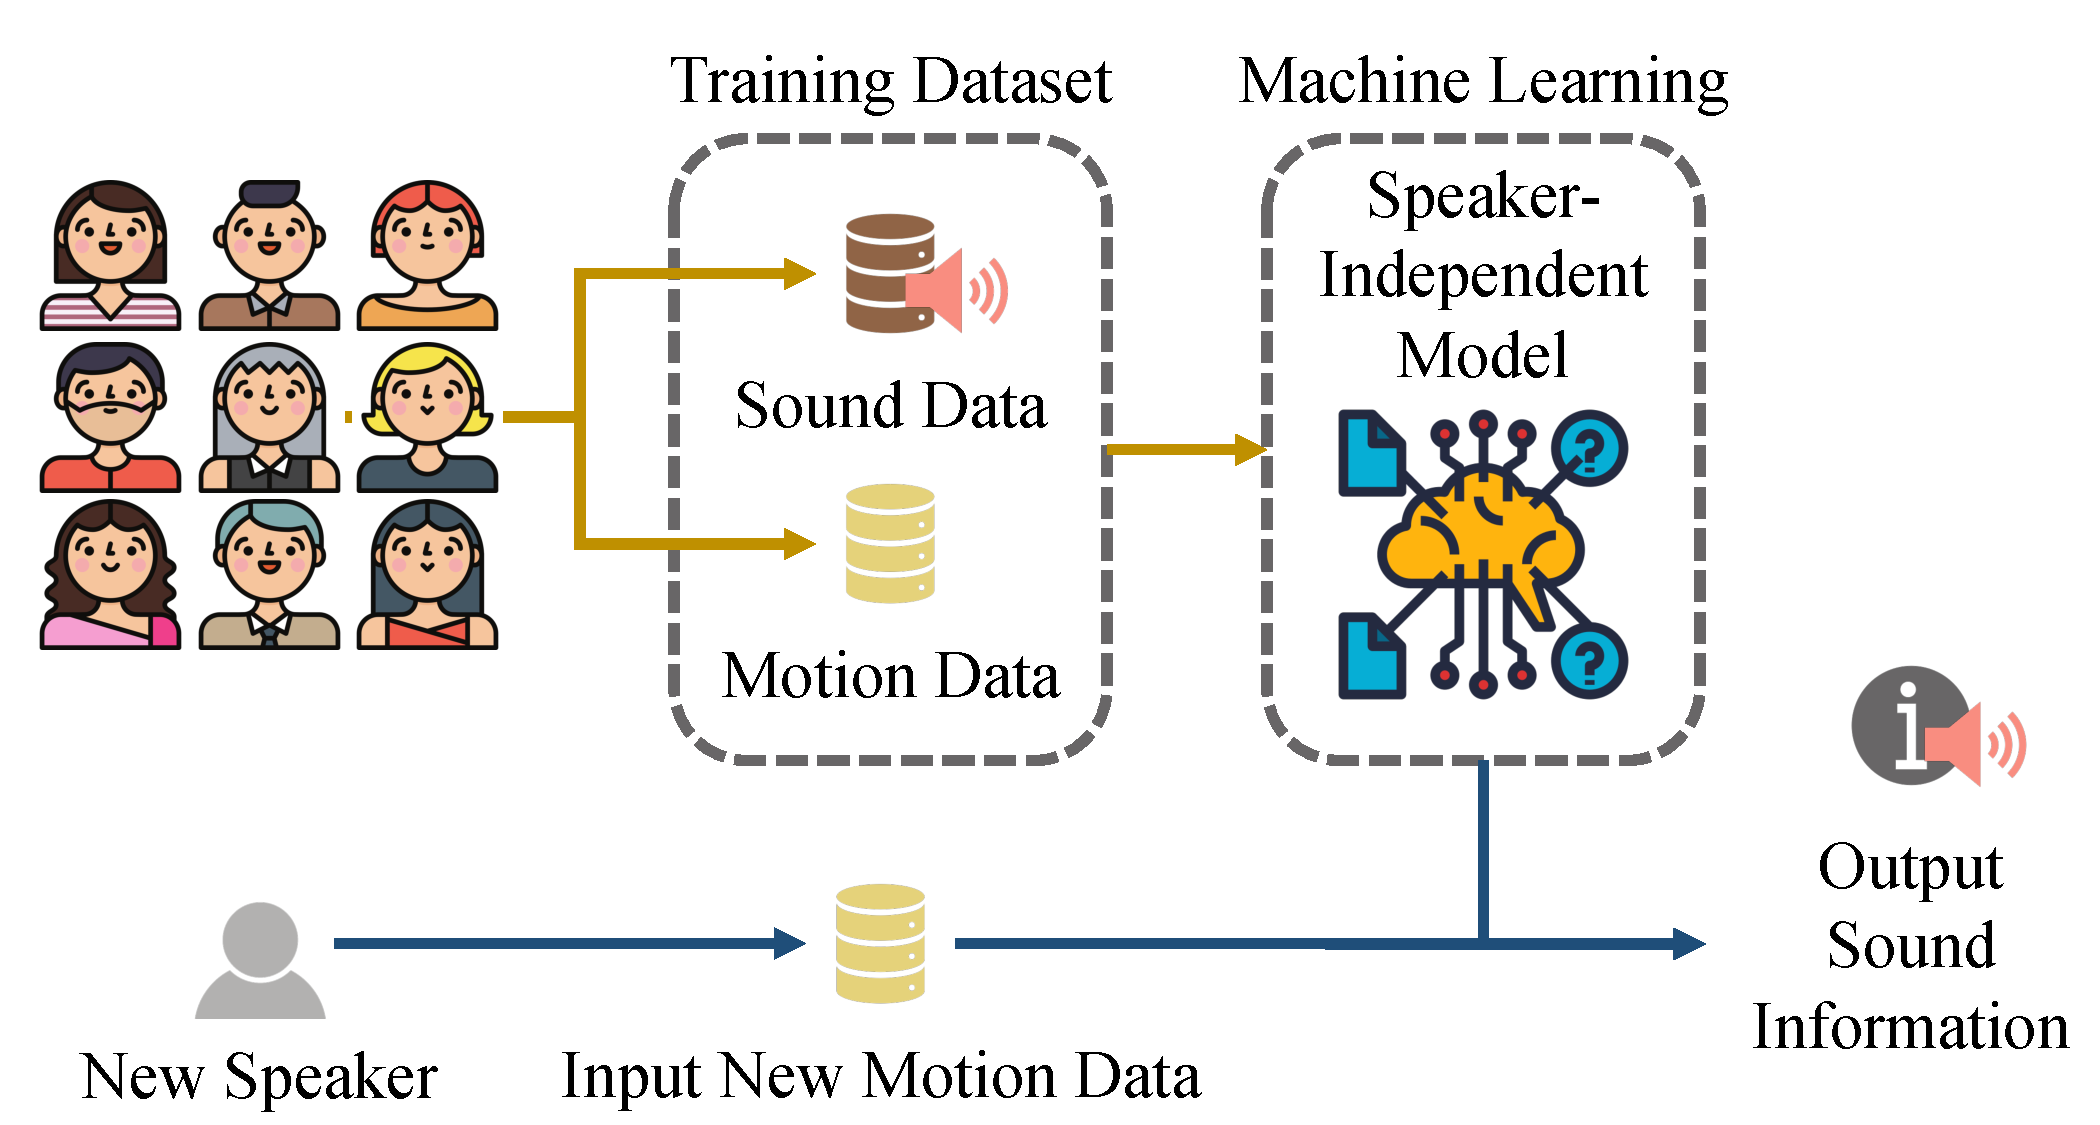
\includegraphics[width=\textwidth]{speakerIndependent}
				\subcaption{Speaker-Independent: the model is trained on a group of speakers, and can be used to predict brand new speakers.}
%			\end{subfigure}
		\end{minipage}
		\caption{{\attackName} Attack Should be Speaker-Independent.} \label{fig:depend}
	\end{figure*}
\end{landscape}

%We conquer the challenges by various  signal processing techniques 

%In summary, our contributions are listed as follows.
%This dissertation offers the following contributions:
%The main contributions are summarized as follows:
%
In summary, our main contributions are as follows:
\begin{itemize}
	\item 
	We uncover a new stealth attack named the {\attackName} attack that eavesdrops on smartphones' built-in speakers by the intra-device motion sensors. Existing techniques in Gyrophone~\cite{michalevsky2014gyrophone} and AccelWord~\cite{zhang2015accelword} cannot be used for the {\attackName}  attack because their system are speaker-dependent, which require the training speech data from the victim. The {\attackName}  attack, however, removes this requirement and thus is more dangerous and harmful.
	
	\item 
	To the best of our knowledge, we are the first to apply compressed sensing theories in the audio-to-motion side-channel data so as to bridge the gap between sampling rates. This is the core technique we used to achieve speaker-independent of the attacking system.
	
	
	\item 
	We design the {\systemName} system and validate its feasibility on learning user activity, speaker gender/identity, and speech content.  {\systemName} system can achieve higher accuracy than existing works. In addition, we have studied how different internal parameters (used in algorithms) and external parameters (properties of input data) affect the  performance of this system.
	
	
%	\item User-independent no individual training
%	
%	Unnoticeable, universal
\end{itemize}


















%%%%%%%%%%%%%%Materials%%%%%%%%%%%%%%



%~\cite{aaaGoogleSearch,michalevsky2014gyrophone,matyunin2018zero}

%
%Any app installed on a smartphone  is permitted to access to motion sensors 


%the system automatically grants the app that permission at install time. 
%%TODO side channal attack??

 
%Why can smartphones provide so many efficient and user-friendly applications? Because these smart devices seamlessly integrate the physical world with the cyber world via their sensors (e.g., light, accelerometer, gyroscope, microphone, speaker, camera, GPS, etc.)~\cite{sikder20176thsense}.
%
%
%
%However, the presence of sensors also has the dark side: \textit{sensor-based attack}s on smartphones. 
%
%The feasibility of keystroke inference from nearby key- boards using accelerometers has been shown in [35]. In [21], the authors demonstrate the possibility of keystroke inference on a mobile device using accelerometers and mention the potential of using gyroscope measurements as well, while another study [19] points to the benefits of exploiting the gyroscope.
%While the number of applications using different sen- sors [38] is increasing and new devices offer more sen- sors, the presence of sensors have opened novel ways to exploit the smart devices [76]. Attackers can exploit the sensors in many different ways [76]: they can trig- ger an existing malware on a device with a simple flash- light [28]; they can use a sensor (e.g., light sensor) to leak sensitive information; using motion sensors such as ac- celerometer, and gyroscope, attackers can record or steal sensitive information from other nearby devices (e.g., computers, keyboards) or people [10, 87, 26, 42]. They can even transfer a specific malware using sensors as a communication channel [76]. Such sensor-based threats become more serious with the rapid growth of Apps uti- lizing many sensors [6, 2].
%
%
%In fact, these sensor-based threats highlight the flaws of existing sensor management systems used by smart devices. Specifically, Android sensor management sys- tem relies on permission-based access control, which considers only a few sensors (i.e., microphone, camera, and GPS)1. Android asks for access permission (i.e., with a list of permissions) only while an App is being installed for the first time. Once this permission is granted, the user has no control over how the listed sensors and other sensors (not listed) will be used by the specific App. Moreover, using some sensors is not considered as a vi- olation of security and privacy in Android. For instance, any App is permitted to access to motion sensors by just accessing the sensor API. Access to motion sensors is not controlled in Android.


%Android sensor management
%
%In this paper, we show how to use only motion sensors to eavesdrop on everything played by the smartphones' built-in speakers, i.e., how to turn the existing over 3 billion smartphones to billions of spy-phones.
%
%This attack is based on the fact that...


%Four  papers: Gyrophone, WALNUT, AccelWord, Speechless
%
%
%
%spy bugs and listening devices
%
%Smartphones are everywhere. 
%
%
%
%
%Existing Eavesdropping on smartphones
%
%Prior work like gyrophone and accelword


% Smartphones are everywhere.
%
%versatile handheld devices have become indispensable tools,
%
%Generally, older "feature" phones are capable of voice calls, text messages and the occasional photo, but not much else. Smart phones, on the other hand, are essentially handheld computers. Users can check their email, browse the web, post updates to social media sites, play games, listen to music, watch movies and even shoot video.
%
%The capabilities are so extensive, 
%
%
%From teenagers to seniors, people 
%
%
%However, the ubiquity of smartphones not only bring convenience to legitimate users, but also build a hotbed of new types of attacks.
%
%According to reports issued by several market-research firms,  including Forrester Research, the total number of smartphone users worldwide will reach 3 billion this year—40 percent of the human population. 
%
%Who doesn’t own a Smartphone? Right from teenagers to senior citizens and from businesspersons to business leaders, Smartphone ownership is Ubiquitous and all pervasive. Indeed, it is estimated that nearly 80\% of the world’s population is now connected to each other through the mobile phones with Smartphones constituting the majority of such devices.
%
%
%
%THE dawn of the planet of the smartphones came in January 2007, when Steve ... The smartphone is ubiquitous, addictive and transformative .
%
%
%The Smartphone is everywhere. Its Ubiquity has resulted in new forms of capitalism with Entrepreneurs and Traders using it for direct communication and  ...
%
%
%According to reports issued by several market-research firms, including Forrester Research, the total number of smartphone users worldwide will reach 3 billion this year—40 percent of the human population. For many, these versatile handheld devices have become indispensable tools, providing connections to loved ones, entertainment, business applications, shopping opportunities, windows into the greater world of social media, news, history, education, and more. And of course, they can always be put to use for a quick selfie. With so many devices in so many hands now, the visual landscape has changed greatly, making it a rare event to find oneself in a group of people anywhere in the world and not see at least one of them using a phone. Collected here: a look at that smartphone landscape, and some of the stories of the phones’ owners.

%
\section{Background}

\subsection{Voice Acoustics}\label{sec:voice}

The generation of human voice follows a source-filter model~\cite{fant1960acoustic}. A speech signal can be seen as a source signal (the glottal source at the larynx, or noise generated at a constriction in the vocal tract), filtered with the resonances in the cavities of the vocal tract (tongue, teeth, lips, velum etc. modifying the sound spectrum over time). This theory has been verified using 3-D printed models of two configurations of a vocal tract to generate sounds to generate the vowels in the words ``had'' and ``heard''~\cite{wolfe2016experimentally}. 

%TODO choose one
%The fundamental frequency for speech ($f_0$) is typically 80 to 250 Hz.
A typical adult male will have a fundamental frequency  ($f_0$) of from 85 to 155 Hz, and that of a typical adult female from 165 to 255 Hz~\cite{baken1987clinical,titze1994principles}. The frequencies of the first, second and $i$-th resonances are labeled as  $R_1, R_2, \ldots R_i$, and those of the spectral peaks produced by these resonances are called formants, $F_1, F_2, \ldots F_i $~\cite{titze2015toward}. 

According to~\cite{ladefoged2014course}, English vowels are perceived largely according to the values of the formants $F_1$ and $F_2$. The range of $F_1$ is roughly from 270 to 860 Hz, and that of $F_2$ from 840 to 2790 Hz~\cite{peterson1952control}. As for English consonants, there are six categories: plosive/stop (e.g. /p/), fricative (e.g. /f/), affricate (e.g. /dZ/), nasal (e.g. /m/), lateral (e.g. /l/), and approximant (e.g. /r/). The frequencies of consonants vary a lot. The turbulence of /s/ and /z/ occurs above 3500Hz, and reaches as high as 10,000 Hz, whereas /w/ has $F_1$ from 250 to 450 Hz and $F_2 $ from 600 to 850 Hz~\cite{ladefoged2012vowels}. 

\begin{table*}[h]
	\centering
	\caption[]{Maximum Sampling Rate of Smartphone Sensors}
	%	\footnote{Some part of the data is from~\cite{matyunin2018zero}, others are tested }
	\label{tab:samplerate}
	\begin{tabular}{lccc} %{lp{2cm}p{2cm}}
		\toprule		
				\multirow{2}{3cm}{Device}& \multirow{2}{2.5cm}{Release Year } & Microphones'  & Motion Sensors'  \\
	& & Sampling Rate & Sampling Rate\footnotemark \\
		\midrule
		Samsung Galaxy S8 & 2017 & 192,000 Hz & 500 Hz\\
		Samsung Galaxy S7 & 2016 & 192,000 Hz & 500 Hz\\		
		Google Nexus 6P & 2015 & 48,000 Hz & 400 Hz\\
		LG Nexus 4 & 2012 & 48,000 Hz& 200 Hz\\
		\bottomrule
	\end{tabular}
\end{table*}
\footnotetext{Data is partially from~\cite{matyunin2018zero} and partially by calling the \texttt{getMinDelay()} function of \texttt{android.hardware.Sensor} class. In fact, the sensors can sample at a higher rate, but the operating systems restrict this rate in order to save power or for security concerns. For example, Google Nexus 6P uses Bosch BMI160, whose sampling rate can be 1600 Hz., but Android operating system only supports up to 400 Hz on the phone.}


By Nyquist–Shannon sampling theorem, to properly sample a signal contains no frequency components higher than $f$ Hz, the sampling rate must be at least $2f$ Hz (Nyquist rate). In other words, a sampling rate of 400 Hz (motion sensors' rate of Google Nexus 6P as shown in Table~\ref{tab:samplerate}) can only handle signals whose component frequencies are below 200 Hz. Except for part of the fundamentals, all $F_1$ and $F_2$ frequencies can not be sensed. Therefore, it is impossible to perceive the signals with such a low sampling rate.

Fortunately, the objective of using motion data in {\shortname} is liveness detection and user identification, not signal recovery. With some proper machine learning technology, the undersampled data is informative enough to fulfill the purpose. The reason is, in signal processing, there exists the aliasing phenomenon that high frequency data will have aliases at the low frequency range, which indicates that the information is kept, though distorted.

%Fortunately, thanks to the aliasing  phenomenon and self demodulation effect, the undersampled motion data still contains partial information, which can be used for liveness detection and user authentication .


%\subsection{Aliasing}
%Aliasing is a phenomenon that causes different signals to become indistinguishable (or aliases of one another) when sampled. For a sinusoid of frequency $f$ , sampled with frequency $f_s$, the resulting samples are indistinguishable from those of another sinusoid of frequency $\mid f − N \cdot f_s\mid$ , for any integer $N$. 
%
%Aliasing is an effect that causes different signals to become indistinguishable from each other during sampling. Aliasing is characterized by the altering of output compared to the original signal because resampling or interpolation resulted in a lower resolution in images, a slower frame rate in terms of video or a lower wave resolution in audio. Anti-aliasing filters can be used to correct this problem.


\subsection{Self Demodulation}
Motion sensors not only captures the original sound data, but also captures the modulated signals. In detail, with self demodulation~\cite{berktay1965possible}, the original sounds self interacts  inside  human body,  resulting in sounds with  lower frequency.

\begin{figure}[h]
	\centering
		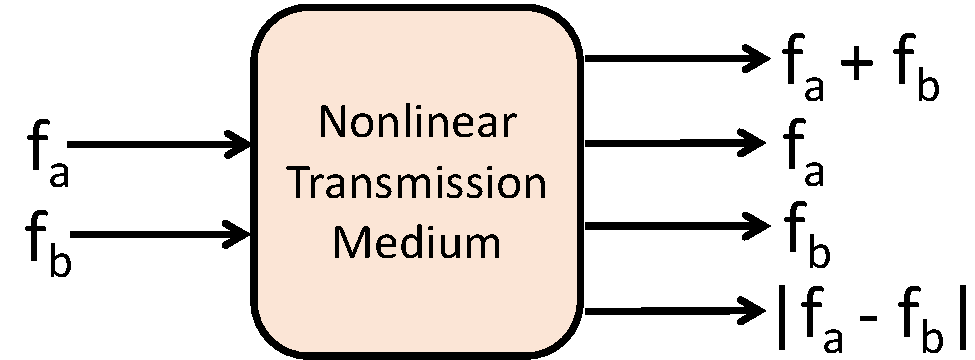
\includegraphics[width=.6\linewidth]{modulation}
	\caption{Self Demodulation of Sound Signals  When Transmitting Through the Human Body.}
	\label{fig:modulation}
\end{figure}

Researchers have found that sounds with different frequencies that transmitted through a nonlinear medium would interact with each other~\cite{pompei1998use}. This interaction produces new frequencies upon the combination of the sums and differences of the individual frequency components by Khokhlov-Zabolotskaya-Kuznetsov(KZK) parabolic nonlinear wave equation~\cite{novikov1987nonlinear}. 

Since the acoustic impedance of the human body is similar to that of water~\cite{kim2014sound}, the self-demodulation would occur in the human body as show in Fig.~\ref{fig:modulation}. 
The original sound signals with frequency $f_a$ and $f_b$ would introduce two more signals with frequency $f_a + f_b$ and $|f_a - f_b|$. For different person, the original signals generated have different frequency, so the low frequency signal $|f_a - f_b|$ are different, which can be utilized for user authetication.
%
Moreover, note that electronic devices has different acoustic property from that of human body. Therefore, those low frequent signals can be used for liveness detection.

%However, borrowing theories from \textit{compressed sensing}, the {\systemName} system can partially reconstruct the signal and obtain critical information such as the numbers appeared in a conversation, genders or even identities of the speakers, etc., from motion sensor readings, as discussed in Section~\ref{sec:threat}.

\subsection{Acoustic Attenuation}
Another effect helps {\shortname} to do spoof-proof authentication is the acoustic attenuation by human body.
%
It is known that human voice is emitted by the vocal organ and is a combination of mechanical vibrations with multiple  amplitudes and different  frequencies.
%
When a person speaks, the  airflow from the lungs through the trachea compresses the vocal cords causing vibrations to make sounds. The lung, trachea and vocal cord form a resonance chamber. 
%\begin{figure}[h]
%	\centering
%		\includegraphics[width=.4\linewidth]{background}
%	\caption{Background}
%	\label{fig:background}
%\end{figure}

Suppose the length of vocal cords is $d$, the lung volume is $V_0$ and the cross-sectional area at the vocal cords is $S$. According to the polytropic process equation, when the airflow moves $d$, the air pressure at the vocal cords can be expressed as follows,
\begin{displaymath}
P_1 = \frac{P_0 \cdot V^\gamma_0 }{(V_0 - d \cdot S)^\gamma},
\end{displaymath}
where $P_0$ is the normal atmospheric pressure, and $\gamma$ is a coefficient about the air specific heat. 
According to the definition of pressure, if the area at the vocal cords is $S_v$,  the force at the vocal cord is,
\begin{displaymath}
F_0 = P_1 \cdot S_v = \frac{S_v \cdot P_0 \cdot V^\gamma_0 }{(V_0 - d \cdot S)^\gamma}.
\end{displaymath}
When the force is applied to the vocal cords, vertical displacement occurs. 
According to the Newton’s second law of motion, we have,
\begin{displaymath}
F(t) = m a(t) + k x(t) + c v(t),
\end{displaymath}
where $F(t)$ is the external force, $v(t)$ is the speed, $x(t)$ is the vertical displacement, $c$ is the damping coefficient, and $k$ is the spring constant and m is the mass. 
The relation can further be explained as,
\begin{equation}
F(t) = m \frac{d^2 x(t)}{d t^2} + k x(t) + c \frac{x(t)}{d t}.
\label{eq:force}
\end{equation}

The vibration during an airflow pass the vocal cords can be separated into two phases. In the first phase, the airflow is passing the vocal cords which is considered to be a forced vibration with constant force $F_0$. After the airflow passed, in the second phase, the pressure of airflow disappears which leaves the system to vibrate on its own and this is called free vibration. In the forced vibration phase, after applying the Fourier transform to both side of e.q.~\eqref{eq:force}, we have,
\begin{displaymath}
\frac{F_0}{j \omega}(1-e^{-j\omega \delta t}) = - \omega^2 m X(\omega) + k X(\omega) + j \omega c X(\omega).
\end{displaymath}
That is,
\begin{displaymath}
X(\omega) = \frac{1-e^{-j\omega \delta t}}{-\frac{j m}{F_0} \omega^3 - \frac{c}{F_0} \omega^2 + \frac{j k}{F_0} \omega},
\end{displaymath}
where $X(\omega)$ is the spectrum of the vertical vibration signal and $\omega$ is the frequency. 
During the horizontal propagation of the vibration signal from the vocal cords to the throat, the vibration suffers from attenuation, and the corresponding model can be stated as follows,
\begin{displaymath}
x_s(t) = x(t) e^{-\alpha d},
\end{displaymath}
where $x_s(t)$ is the vertical displacement at the throat where the vibration has propagated, $x(t)$ is the vertical displacement at the vocal cords, $d$ is the propagation distance, and $\alpha$ is the attenuation coefficient. 
After applying the Fourier transform to both side of e.q.~\eqref{eq:force}, we have,
\begin{displaymath}
X_s(\omega) = X(\omega) e^{-\alpha d}.
\end{displaymath}
Note that $\alpha$ is related to the propagation medium. Wave propagation in body is dispersive by nature, which implies that different frequencies propagate with different attenuation coefficients at different velocities. Roughly speaking, the attenuation is small when the vibration signal propagates through the hard bone, whereas the attenuation is large through the soft tissue. Therefore, vibration waves generated at different positions at throat result in different values of $\alpha$ and $d$, which make the vibration signals unique at different positions. 
After putting all equations together, we obtain,
\begin{displaymath}
X_s(\omega) = \frac{(1-e^{-j\omega \delta t}) e^{-\alpha d}}{(-jm\omega^3 - c \omega^2 + jk\omega)(\frac{(V_0 - d \cdot S)^\gamma}{S_v \cdot P_0 \cdot V^\gamma_0 })}.
\end{displaymath}
For the same location of the human body, $m$, $c$ and $k$ are stable and belong to the same biometric feature. Each person’s lung volume and vocal cords are also different. Therefore, the vibration at the throat of different people can uniquely be identified, which can be leveraged for authentication. The propagation from electronic device to the target smartphone is different from vocal organ through human body. Thus, this effect is also valuable for liveness detection.


%\subsection{Voice Production}
%source-filter model, why our algorithm is user-independent. Similar source, different filter.
%\subsection{Voice Authentication System}
%Attacking (direct/indirect), here we only consider direct.


%



\section{Threat Model in the  {\systemName} System}\label{sec:threat}
%TODO applications

%%TODO
%{attcker vs system}

The attacker's goal is to eavesdrop on everything played by the smartphone speakers  without the user's awareness. 

The attack begins when the user installs a seemingly innocent application, e.g. a car racing game with motion-control steering wheel (tilt the smartphone to steer). 
%
We assume such a disguised app has the access to motion sensors (accelerometers and gyroscopes) as well as the network. This assumption is easy to fulfill since the permissions to motion sensors and the internet are all considered as \textit{normal} permissions by the Android operating system~\footnote{\scriptsize \url{https://developer.android.com/guide/topics/permissions/overview}}. 
%~\cite{onlineoverview}.
In other words, Android automatically grants the app these permissions at installation time. The operating system doesn't prompt the user to grant permissions, and users cannot revoke these permissions. Moreover, almost every smartphone has motion sensors and is able to connect to the Internet. The {\attackName} attack is therefore a threat to every smartphone user.

There is no other requirement for the attacker to conduct a {\attackName} attack. The disguised app just runs in the background and keeps monitoring the motion sensors. Since the power consumption of the motion sensors is very low, the user will not know the motion sensors are in use. In addition, some smartphones are set to be ``Rotation On'' or ``Lift to Unlock", which means the operating system automatically collects motion data, and the {\systemName} system does not introduce extra consumption by using the sensors.

The sensor data are sent back to the attacker over wireless networks. The attacker can choose to transmit data only when the smartphone is connected to Wi-Fi; otherwise, the user may notice the attack through suspicious cellar data usage. The data will be processed at the attacker's end. By utilizing compressed sensing, machine learning and other signal processing techniques, {\systemName} recovers \textit{critical information} from undersampled motion data.
%
The critical information could be, but not limited to,
%\vspace{-.1in}
%, the followings:
\begin{itemize}
	\item
	User activity. Using motion sensor to recognize user activity is not new. However, those activities (e.g., sitting, walking, running or exercising)  are recognized based on different \textit{macro} motions. {\systemName}, on the other hand, is utilizing the \textit{micro} motions caused by speakers. Therefore, {\systemName} can tell whether a user is listening to music or watching an online talk even when the phone seems stationary.Smartphones' built-in speakers are often used for alarms, phone call ringing, music listening, background sound for game playing, and so on. Different activity plays different sound and creates different motion sensor readings. The {\systemName} system can be trained to classify the motion data to these different user activities. Put the matter another way, an attacker can know when the user wakes up, when she receives phone calls, how long she listens to music, or how long she plays games, and so on.
	\item 
	Speaker gender/identity. When the smartphone user has a audio call, video call, or an online meeting with others, the {\attackName} attackers can learn whether the person she talks to is female or male. {\systemName} can also learn how often the user contacts each different person. Moreover, if the attacker could get those people's voice samples (either by recording in public area, or acquiring from social media online, etc.), the attacker can know exactly who they are.
	\item
	Speech content. Another goal for the attacker is to recover the whole speech content by motion sensors. However, considering the tremendous gap between the sampling rate of smartphone speakers and motion sensors, there is still a long way before success. In Section~\ref{sec:design}, as a proof-of-concept, we use digit recognition to demonstrate the design of the {\systemName} system, since the most critical information such as  banking account numbers, credit card information, and certain passwords,  are essentially combinations of digits. In Section~\ref{sec:experiment}, command recognition is also tested.
\end{itemize}

%\vspace{-.1in}
In addition, It is worth mentioning that the {\attackName} attack is built upon a speaker-independent machine learning model and does not require any specific training data from the user. Though with such data, the accuracy might be further improved. Prior works such as Gyrophone~\cite{michalevsky2014gyrophone} and AccelWord~\cite{zhang2015accelword} can only be used in the speaker-dependent case. Using their techniques, the user must obtain the victim's speech first, which is harder to be carried out in reality.

%\begin{itemize}
%	\item User activity. A loudspeaker is commonly used for alarms, phone call ringing, music listening, background sound for game playing, video calling, and so on. Different activity plays different sound and creates different motion sensor readings. {\attackName} system can be trained to classify the motion data to different user activities. Put the matter another way, an attacker can know when the user wakes up, when she receives phone calls, how long she listens to music, or how long she plays games, and so on.
%	\item Speech 
%\end{itemize}


%
%Permissions on sensors
%
%The system doesn't prompt the user to grant normal permissions, and users cannot revoke these permissions.
%
%PatternListener requires the permission to access speaker, microphone, and motion sensors (i.e., accelerometer and gyroscope) as well as network access permission. Most permissions can be granted without user approval, except the permission of accessing the microphone. However, we observe that the permis- sion of accessing microphone is very popular in Android apps. For instance, microphone permissions are required by 55\% social apps and 52\% communication apps in the Google Play marketplace. The details can be found in the appendix. Therefore, it is easy for Pat- ternListener to obtain the permission after it is disguised as an app in these categories.
%
%which ``tilt to steer'', 
%
%motion-control game app.
%
%Meddling with the data occurs using a seemingly innocent application, e.g. a fake flashlight app, within which holds the attacker’s exploit script. 
%We assume the attacker build a 
%
%
%The adversary’s goal is to inject voice commands into the voice controllable systems without owners’ awareness, and execute unauthenticated actions. We assume that adversaries have no direct access to the targeted device, own equipment that transmits acoustic signals, and cannot ask the owner to perform any tasks.
%
%Assumptions
%
%
%Sample rate on Smartphones.
%
%
%No Target Device Access. We assume that an adversary may target at any voice controllable systems of her choices, but she has no direct access to the target devices. She cannot physically touch them, alter the device settings, or install malware. However, we assume that she is fully aware of the characteristics of the target devices. Such knowledge can be gained by first acquiring the device model and then by analyzing the device of the same model before launching attacks.
%No Owner Interaction. We assume that the target devices may be in the owner’s vicinity, but may not be in use and draw no attention (e.g., on the other side of a desk, with screen covered, or in a pocket). In addition, the device may be unattended, which can happen when the owner is temporarily away (e.g., leaving an Amazon Echo in a room). Alternatively, a device may be stolen, and an adversary may try every possible method to unlock the screen. Nevertheless, the adversaries cannot ask owners to perform any operation, such as pressing a button or unlocking the screen.
%Inaudible. Since the goal of an adversary is to inject voice com- mands without being detected, she will use the sounds inaudible to human, i.e., ultrasounds (f > 20 kHz). Note that we did not use high-frequency sounds (18 kHz < f < 20 kHz) because they are still audible to kids.
%Attacking Equipment. We assume that adversaries can acquire both the speakers designed for transmitting ultrasound and com- modity devices for playing audible sounds. An attacking speaker is in the vicinity of the target devices. For instance, she may secretly leave a remote controllable speaker around the victim’s desk or home. Alternatively, she may be carrying a portable speaker while walking by the victim.
%

%
\section{Attack Design}\label{sec:design}


The workflow of the {\attackName} attack in {\systemName} is shown in Figure~\ref{fig:flow}. The system can be separated into two parts: the user side and the attacker side. 
%
On the user side, a smartphone user downloads a seemingly harmless application and installs it on her device. Then the disguised app runs in the background and keeps monitoring the motion sensors. The sensor readings are then uploaded and sent to the attacker. 
%
On the attacker side, there are training steps and prediction steps. The training steps start from a training dataset that contains both sound data and motion data, while the input for prediction steps only contains motion data. 

The training steps first apply compressed sensing techniques on the sound data and build a learned dictionary from audio files, then process the corresponding motion data to remove unwanted signal components. With the preprocessed motion data and a learned dictionary,  the signal is reconstructed to a signal with more samples. Afterward, the reconstructed signal is fed to a Bidirectional Long Short-Term Memory (Bi-LSTM) network to train a classification model. 
The classification labels/classes (e.g. digits, genders, activity types, and so on) is determined by the sound data only.


\begin{landscape}
\begin{figure*}[h]
	\centering
	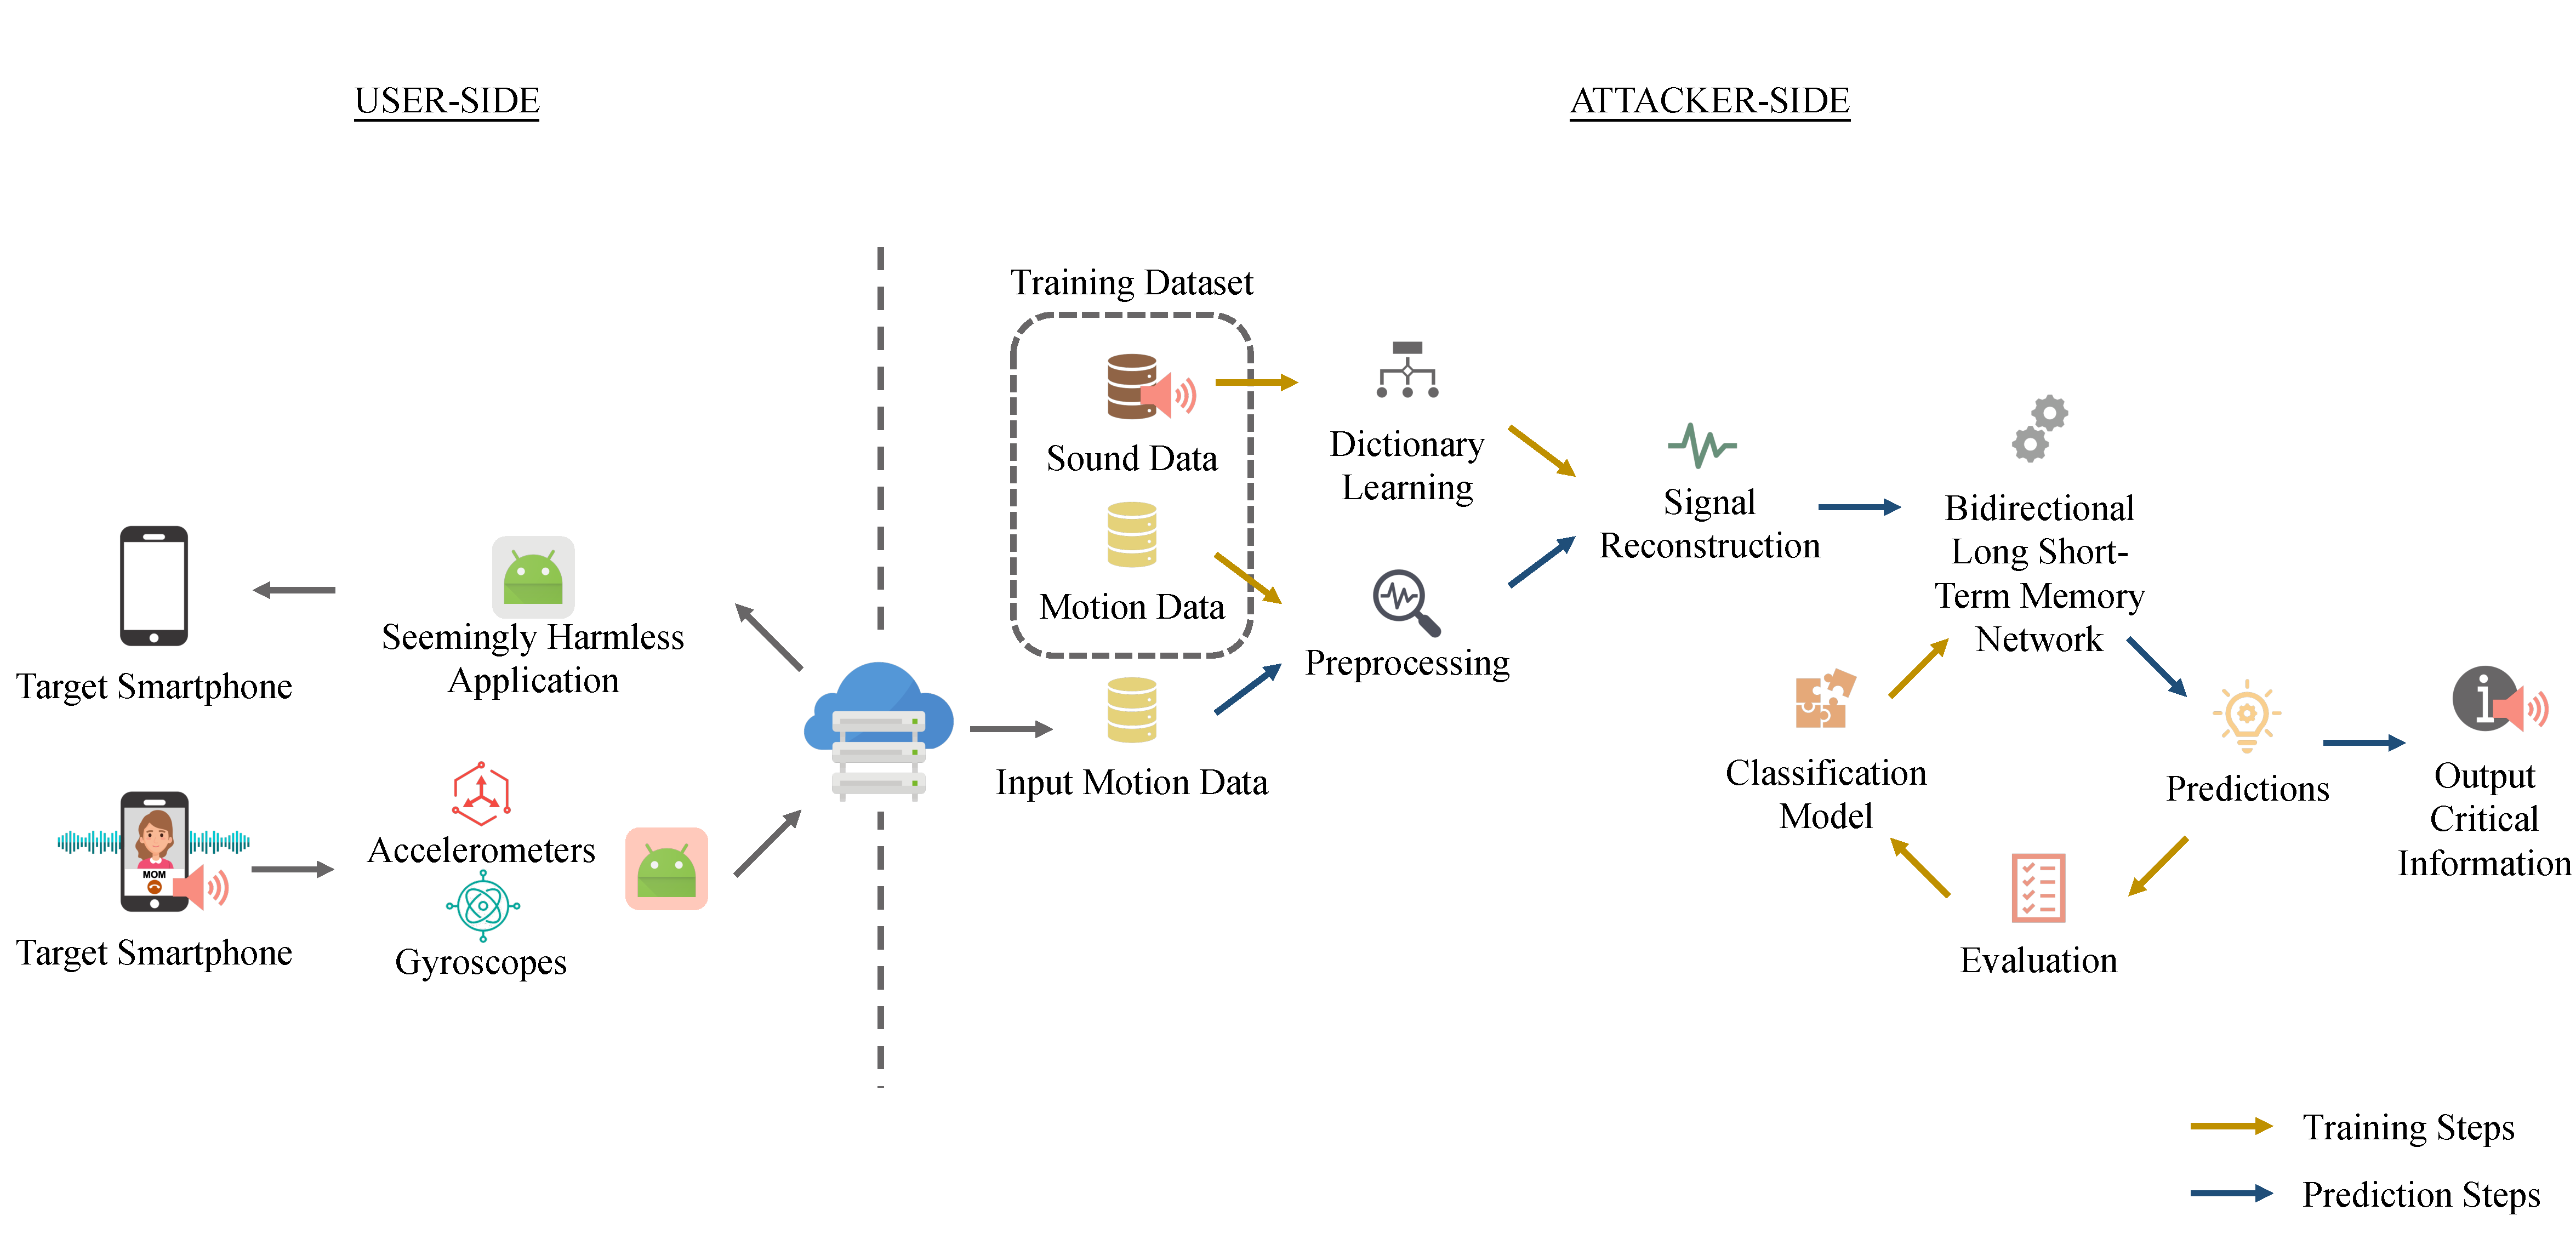
\includegraphics[width=\linewidth]{attackflow}
	\caption{The {\attackName} Attack Workflow in the {\systemName} System. }
	\label{fig:flow}
	%		\vspace{-.2in}
\end{figure*}
\end{landscape}



The prediction steps start with motion data, go by preprocessing, adopt the learned dictionary to reconstruct signals, and finally use the trained Bi-LSTM model to output critical information, without the presence of sound data.



In this section, we explain in detail how the {\systemName} system implements the {\attackName} attack to eavesdrop on digits played by smartphone speakers. A similar approach can be applied to obtain user activity type or speaker gender/identity as evaluated in Section~\ref{sec:experiment}.


\subsection{Training Dataset}

\begin{table}[h]
	\caption{Dataset Information}
	%	\footnote{Some part of the data is from~\cite{matyunin2018zero}, others are tested }
	\label{tab:dataset}
	\centering
	%	\resizebox{\columnwidth}{!}{
	\begin{tabular}{lcc} %{lp{2cm}p{2cm}}
		\toprule		
		%			\multirow{2}{3cm}{Dataset}
		%			& TIDIGITS & Speech Commands\\
		%			& \cite{leonard1993tidigits} & \cite{warden2018speech}\\
		%			
		Dataset & TIDIGITS~\cite{leonard1993tidigits} & Speech Commands~\cite{warden2018speech}\\
		\midrule
		Sampling Rate & 20,000 Hz & 16,000 Hz\\
		No. Speakers & 326 & 2,618\\
		Labels & 11 Digits & 35 Command Words \\
		No. Utterances & 7,172& 105,829\\
		Training Size & 3,586 & 84,843\\
		Validation Size & - & 9,981\\
		Testing Size & 3,586 & 11,005\\
		\bottomrule
	\end{tabular}
	%}
\end{table}

As shown in Table~\ref{tab:dataset}, we use two datasets, TIDIGITS and Speech Commands. 

TIDIGITS~\cite{leonard1993tidigits} are professional recordings of isolated digits, which has been used in~\cite{michalevsky2014gyrophone} and \cite{anand2019spearphone}. Therefore, in the main sessions of this chapter, we illustrated our system using this dataset for the comparison's purpose. However, TIDIGITS only contains digits, and the utterances are all recorded in laboratory conditions. It is natural that the accuracy would be higher on such a dataset. Therefore, we consider another dataset Speech Commands~\cite{warden2018speech}, which is the TensorFlow Speech Commands Dataset(Version 2). This dataset can be used for limited-vocabulary speech recognition. It consists of 105,829 utterances of 35 command words such as up, down, forward, stop, house, happy, etc. This dataset is recorded by a web-based application in a crowd-sourcing manner. Speakers are from all over the world and they speak the commands in uncontrolled environments. Basically, if a model trained on Speech Commands works well, it indicates that any piece of speech recordings online can be used as the training data for the {\systemName} system. The result using this dataset is shown in Section~\ref{sec:word}, the correct rate is 83.2\%.



From now on, we focus on TIDIGITS.


\begin{figure}[H]
	\centering
	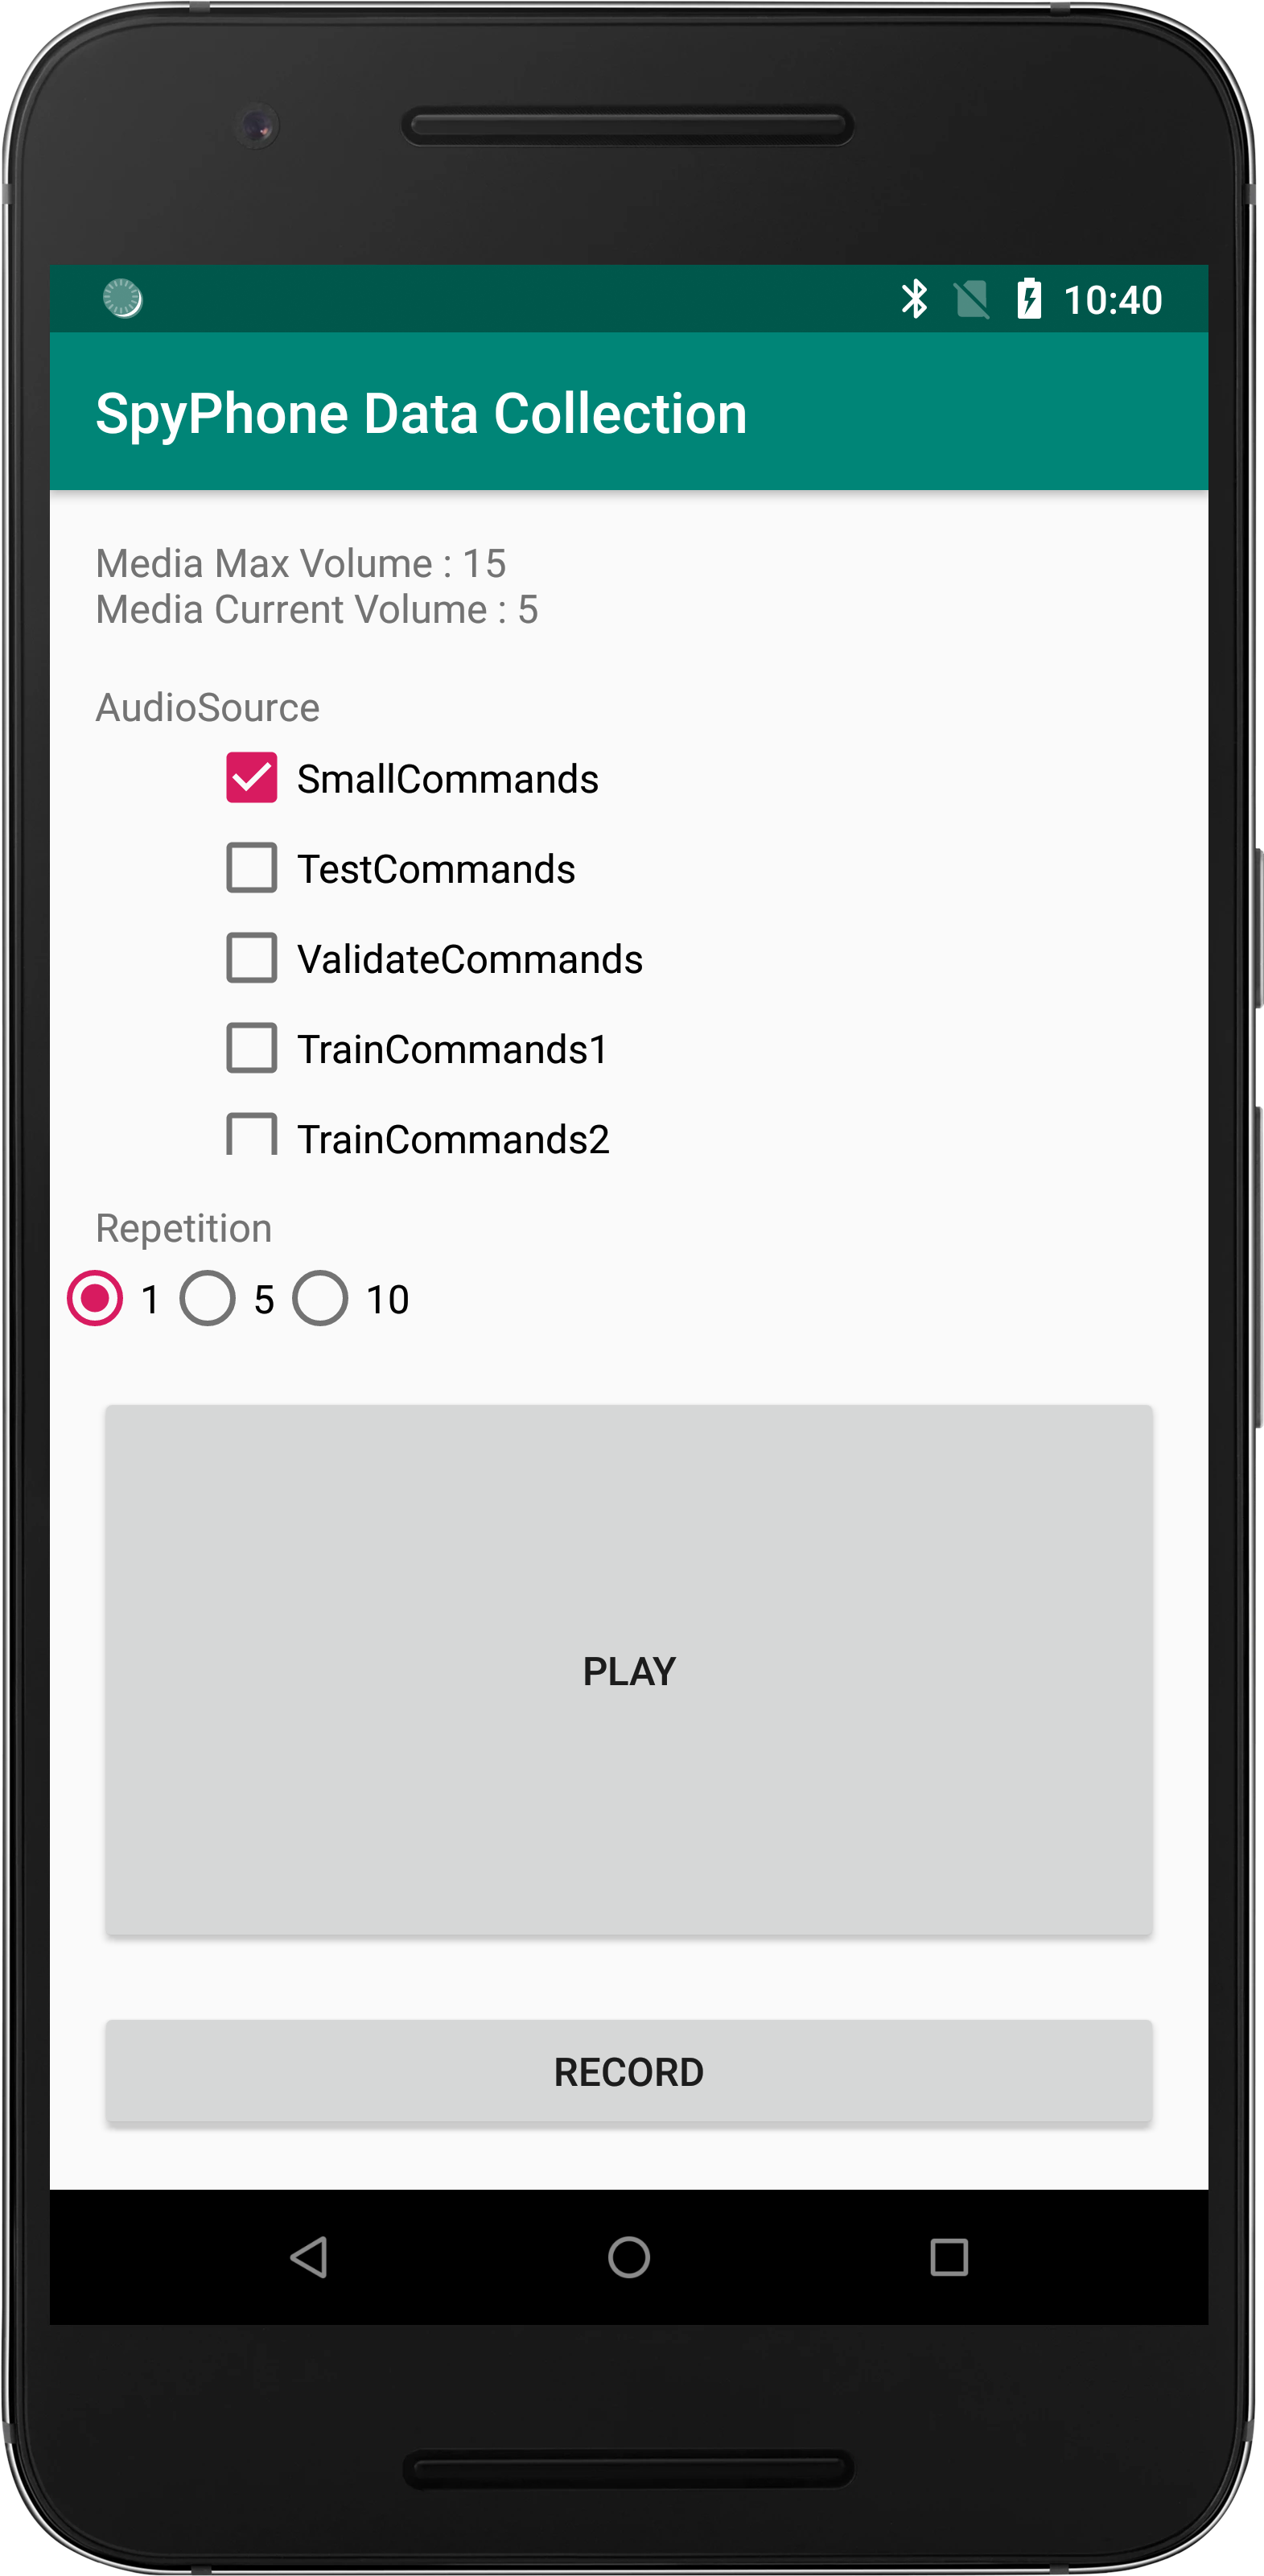
\includegraphics[height=.4\textheight]{SpyPhoneData}
	\caption{{\spp} Data Collection Application}
	\label{fig:spyphoneapp}
\end{figure}

In the beginning, the TIDIGITS dataset is used to build both the sound data and the motion data for the training dataset.
%
This corpus contains speech of 11 isolated digits: ``one'', ``two'', \ldots, ``nine'', ``zero'' and ``oh'', which are collected using an Electro-Voice RE-16 Dynamic Cardiod microphone, digitized at 20,000 Hz.
%
These audio files are directly used as training sound data. 
The motion data, however, are collected by playing these audio files using the built-in speakers of a Google Nexus 6P device. They are the simultaneous recordings from the same phone's  accelerometers and gyroscopes with a sampling rate of 400 Hz.
When playing the sound, the volume is set to be the highest level since these data will be used for training and the higher volume, the higher accuracy (according to experiments in Section~\ref{sec:impact:volume}).
Note that when the {\attackName} attack is conducted in practice, the input motion data may come from a lower volume setting defined by the user. The attacker cannot control the volume setting of the target smartphone, but she can control the volume when building the training dataset. 
%
For the training dataset, only part of the sound and motion data are used. The impact of the training data size on the prediction accuracy is elaborated in Section~\ref{sec:impact:trainsize}.
All data are collected by the SpyPhoneApp as shown in Figure~\ref{fig:spyphoneapp}.



 \begin{algorithm}[!t]
	\small
	\DontPrintSemicolon
	\LinesNumbered
	\SetKw{KwRead}{audioRead}
	\SetKw{KwRemove}{removeSilence}
	\SetKw{KwKVSD}{kvsd}
	\SetKw{KwShift}{shiftLeft}
	\SetKw{KwDown}{downSample}
	\SetKw{KwBuffer}{buffer}
	\SetKw{KwConca}{concatenate}
	\KwIn{Training Sound Dataset $\mathcal{T}_i$ for class $i$, Downsample Rate $r$, Dictionary Size $(N, K)$ }
	\KwOut{Dictionary $D_i$ for class $i$}
	$ S_i \leftarrow []$ \tcp*{Initialize training vectors} 
	\ForEach{audio file $\tau$ in $\mathcal{T}_i$}{
		\tcp{get signal $s$ and sampling frequency $fs$}
		$[s, fs] = \KwRead(\tau)$\;  
		\tcp{remove unvoiced part}
		$s\leftarrow  \KwRemove(s)$\;
		\tcp{downsample signal to $r$ subsignals and buffer each subsignal of length $N$}
		\ForEach{$j$ from 1 to $r$}{
			$s \leftarrow \KwShift(s, 1)$  \tcp*{shift left by 1 sample}  \label{line:shift}
			$ss \leftarrow \KwDown(s, r)$\; \label{line:down}
			$bs \leftarrow \KwBuffer(ss, N)$  \;
			$S_i \leftarrow \KwConca(S_i, bs)$
			
		}
		
	}
	\tcp{run K-SVD dictionary training algorithm}
	$D_i \leftarrow \KwKVSD(S_i, N, K)$
	\caption{{BuildDictionary}\label{algo:builddic}}
\end{algorithm}

\subsection{Dictionary Learning}\label{sec:design:dict}

\begin{figure*}[ht]
	\centering
	\includegraphics[width=.55\linewidth]{dict}
	\caption{Example of Learned Dictionary Atoms. For each digit class, two different atoms are shown.}\label{fig:atoms}
\end{figure*}

We now demonstrate how to construct efficient representations of audio files by building a dictionary learned from the data itself. 
Recall Section~\ref{sec:compressed}, a learned dictionary is used to reconstruct a signal when it is undersampled. 
%
In the {\systemName} system, the sound data are the signals of interest while the motion data are the measurements. The training sound data are grouped into 11 classes, (one to nine, zero, and oh). For each class $i$, the dataset is denoted by $\mathcal{T}_i$ and the representation dictionary $D_i$ is computed by Algorithm~\ref{algo:builddic}.

As shown in Figure~\ref{fig:compressed}, each representation dictionary $D_i$ is a collection of $K$ atoms, where each atom is a column vector of length $N$. An atom is basically some typical patterns of the signal of interest. For sound signal $s_i$ of class $i$,
it should be represented or approximated as a linear combination of some few of the dictionary atoms. Mathematically,
%\begin{displaymath}
	$s_i = D_i * w_i,$
%\end{displaymath} 
for each column $s_i$ in $S_i$. Here $S_i$ is the training vectors calculated in Algorithm~\ref{algo:builddic}. Compared to the original sound signal from an audio file, $S_i$ is the result from many functions including \verb|removeSilence()|, \verb|downSample()|, and \verb|buffer()|. 
 
 
 
Note that the length of a dictionary atom must be the same as the length of the training vector $s_i$. Since the original sound signal can have at most 2 s $\times$ 20,000 Hz = 40,000 samples (The duration of audio files in the dataset is at most 2 seconds.). If directly using original sound to train the dictionary, the atom size must be 40,000 as well. However, not all signals in an audio file are informative. By applying \verb|removeSilence()|, the unvoiced part of the audio signals is removed, which significantly improves the space and time efficiency of the algorithm. The \verb|removeSilence()| is based on \cite{rabiner2011theory}, which calculates the short-time energy of signals and conducts zero-crossing analysis to differentiate sounding and unvoiced parts.
 
 

Moreover, from voice acoustics elaborated in Section~\ref{sec:voice}, the most informative frequency range is roughly 100-4000~Hz, the 20,000~Hz sampling rate oversamples human speech. Therefore, to build a better representation dictionary, we shift the signals (Line~\ref{line:shift} in Algorithm~\ref{algo:builddic}) and downsample it (Line~\ref{line:down} in Algorithm~\ref{algo:builddic}) by keeping the first sample and then every $r$-th sample after the first. The impact of the downsample rate $r$ is evaluated in Section~\ref{sec:impact:downrate}.

Last but not least, different people say different digits with intrinsically different time duration, which results in different signal lengths. To build a general representation dictionary, we buffer every signal with the fixed buffer size as $N$ using \verb|buffer()|. In other words, no matter how long is the original sound signal, by Algorithm~\ref{algo:builddic}, it is transformed into a matrix $S_i$ with $N$ rows. The number of columns, however, is not fixed. For convenience's sake, we denote this number as $L_i$.




 
Dictionary Learning is the process of finding a dictionary, $D_i$ of size $N \times K$, and a corresponding coefficient matrix $W_i$ of size $K \times L_i$ such that the approximations of the training vectors, $S_i$ of size $N \times L_i$, are as good as possible, given a sparseness criterion on the coefficients. Mathematically, the dictionary learning problem can be formulated as an optimization problem with respect to $D_i$ and $W_i$:
%$
\begin{displaymath}
	\left\lbrace 
	D_{i, opt},
	W_{i, opt}
	\right\rbrace 
	=
	\argmin_{D_i, W_i}
	\sum_{l=1}^{L_i}
	\left( 
	\gamma
	\Vert w_{i, l} \Vert_p
	+
	\Vert s_{i,l} - D_i w_{i, l} \Vert_2
	\right) 
	,
%	$
\end{displaymath}
where $\gamma$ and $p$ are as in Eq.~(\ref{eq:reconstruction}), $s_{i, l}$ is the $l$-th column of $S_i$, and $w_{i, l}$ is the $l$-th column of $W_i$. 




The solver we use for this optimization problem is K-SVD~\cite{aharon2006k}, as it is one of the most well-known shared dictionary learning algorithms~\cite{xu2017survey}. We did not test all existing dictionary learning algorithms, but among those we tested, PCA~\cite{haykin2007neural}, K-SVD,  and GAD~\cite{jafari2011fast}, K-SVD provides the best results. 




K-SVD is an iterative method with two main steps: First, keep $D_i$ fixed then solve $W_i$, which is essentially $L_i$ separate problems as in Eq.~(\ref{eq:reconstruction}); Second, keep only non-zero positions in $W_i$ fixed and find $D_i$ and $W$ using singular-value decompositions (SVD). Figure~\ref{fig:atoms} shows the first two atoms in the learned dictionary of each digit class using K-SVD. Generally, the atoms are different inter-class and similar intra-class.

By concatenating every $D_i$ together, the overall dictionary is 
\begin{equation}
	D = \left[ D_1, D_2, \ldots, D_i, \ldots, D_{11} \right], \label{eq:dictConcat}
\end{equation}
which will be used for signal reconstruction in later steps.





\subsection{Motion Data Preprocessing}
The input motion data are collected similarly to how motion data are collected for the training dataset, i.e., playing TIDIGITS audio files by the smartphone's built-in speakers. However, since these data are to simulate the attacking scenarios in reality, the data are collected multiple times using 15 different volume settings (Section~\ref{sec:impact:volume}). Moreover, we collected the motion data in both quiet and noisy environment (Section~\ref{sec:impact:noise}), and in both stable and moving states (Section~\ref{sec:impact:move}).
\begin{figure*}[!h]
	\centering
	\includegraphics[width=.8\linewidth]{preprocess0}
	\caption{The Magnitude and Phase Response of the FIR Highpass filter.}\label{fig:spyphoneresponse}
\end{figure*}


\begin{figure}[H]
	\begin{minipage}[t]{.45\linewidth}
		\centering
		\includegraphics[width=\linewidth]{preprocess1}
		\includegraphics[width=\linewidth]{preprocess2}
		\vspace{-.2in}
		\subcaption{Raw Motion Data.}\label{fig:rawmotion}
		\vspace{.2in}
		\includegraphics[width=\linewidth]{preprocess3}
		\vspace{-.2in}
		\subcaption{Spectrogram of Raw Motion Signals.}\label{fig:rawspec}
	\end{minipage}
	\begin{minipage}[t]{.05\linewidth}
		\quad
	\end{minipage}
	%\end{figure}
	%
	%\begin{figure}\ContinuedFloat	
	\begin{minipage}[t]{.45\linewidth}
		\centering
		\includegraphics[width=\linewidth]{preprocess4}
		\vspace{-.2in}
		\subcaption{Spectrogram of Proceseed Signals.}\label{fig:newspec}
		\vspace{.2in}
		\includegraphics[width=\linewidth]{preprocess5}
		\includegraphics[width=\linewidth]{preprocess6}
		\vspace{-.2in}
		\subcaption{Preprocessed Motion Data}\label{fig:newmotion}
	\end{minipage}
	
	\caption[Preprocessing of Motion Data. ]{Preprocessing of Motion Data. The top two figures show the raw data from 3-axis accelerometers and 3-axis gyroscopes. There are 450 samples shown in the figure. These samples span about one second (450 / 400Hz = 1.125s) and are collected when the user is dropping the head of the phone while playing a ``Zero'' utterance from a male speaker. The frequency of such movement is far less than the frequency of human voices. Therefore, by applying the high pass filter, the noise caused by hand movements will be removed. }
	
	\label{fig:spyphonepreprocess}
\end{figure}

As mentioned in Section~\ref{sec:intro}, the motion data is impeded by low sampling rates, weak target signals, and large  interference  noises. To overcome such problems, we must preprocess the motion data. We apply a high pass filter to mitigate the noise and increase the signal-to-noise ratio. The cutoff frequency is set to be 50 Hz, since noises such as walking or other human body movements are unlikely to generate signals as high as 50 Hz.
We also use the speech-background separation algorithms from \cite{rabiner2011theory} to differentiate the data affected by sound signals from those do not. The red vertical lines in Figure~\ref{fig:rawmotion} are the borderlines between the speech part and the background part. 
Figure~\ref{fig:rawspec} and Figure~\ref{fig:newspec} show that various noises can be removed by applying a high pass filter.
The result after the preprocessing stage is shown in Figure~\ref{fig:newmotion}. These data will be used in the next signal reconstruction stage.



\subsection{Signal Reconstruction}
In this stage, the preprocessed motion data will be used to reconstruct the original audio data.

Mathematically, the goal of signal reconstruction is to solve $w^\prime$ in 
%$$$$ 
%\vspace{-.2in}
%\begin{displaymath}
	$x = R \times w^\prime$
%\end{displaymath}
as in Figure~\ref{fig:compressed}. Here the measurement $x$ is the motion data after preprocessing, and the reconstruction matrix $R$ is calculated by
\begin{equation}
R = S \times D, \label{eq:reconstruct2}
\end{equation}
where $S$ is the sensing matrix and $D$ is the dictionary obtained in Section~\ref{sec:design:dict}.

In the {\systemName} system, the sensing matrix describes the sensing procedure from audio data to motion data, which can be regarded as a downsampling operation. The downsampling rate ($r$) is determined by the sampling frequencies of smartphone speakers ($f_1$) and motion sensors ($f_2$): $r = f_1/f_2$. For example, a sensing matrix with downsample rate $r=3$ is as follows:
\begin{displaymath}
\small
S = 
\begin{bmatrix} 
1 & 0 & 0 & 0 & 0 & 0 & 0 & \cdots & 0  & 0& 0\\
0 & 0 & 0 & 1 & 0 & 0 & 0 & \cdots & 0 & 0& 0\\
0 & 0 & 0 & 0 & 0 & 0 & 1 & \cdots & 0 & 0& 0\\
\vdots & \vdots & \vdots & \vdots & \vdots & \vdots & \vdots &  & \vdots & \vdots & \vdots\\
0 & 0 & 0 & 0 & 0 & 0 & 0 & \cdots & 1 & 0& 0\\       
\end{bmatrix}.
\end{displaymath}
%
In the {\systemName} system, the true value of this rate can be as high as 48,000~/~ 400~ = 120, which indicates a huge information loss and a big challenge to recover the signals.
%
Note that Algorithm~\ref{algo:builddic} also has a downsampling operation (Line~\ref{line:down}), therefore the $R=S \times D$ operation can be replaced by changing the parameter $r$ in Algorithm~\ref{algo:builddic}. When reconstructing the signals, $D$ is used as $R$. The impact of the downsample rate $r$ is evaluated in Section~\ref{sec:impact:downrate}.
%
To solve Eq.~(\ref{eq:reconstruct2}), GPSR~\cite{figueiredo2007gradient} is used, which is able to find  
$
%\begin{displaymath}
w^\prime_{opt}
=
\argmin_{w^\prime}
\left( 
\gamma
\Vert w^\prime \Vert_p
+
\Vert x - R w^\prime \Vert_2
\right)
. 
$
%\end{displaymath}
The last step is to reconstruct the signal of interests by
$
%\begin{displaymath}
s^\prime = D \times w^\prime_{opt}.
%\end{displaymath}
$
These signals will be used as training data for the Bi-LSTM network discussed in the next section.




\begin{figure}[!b]
	\centering
	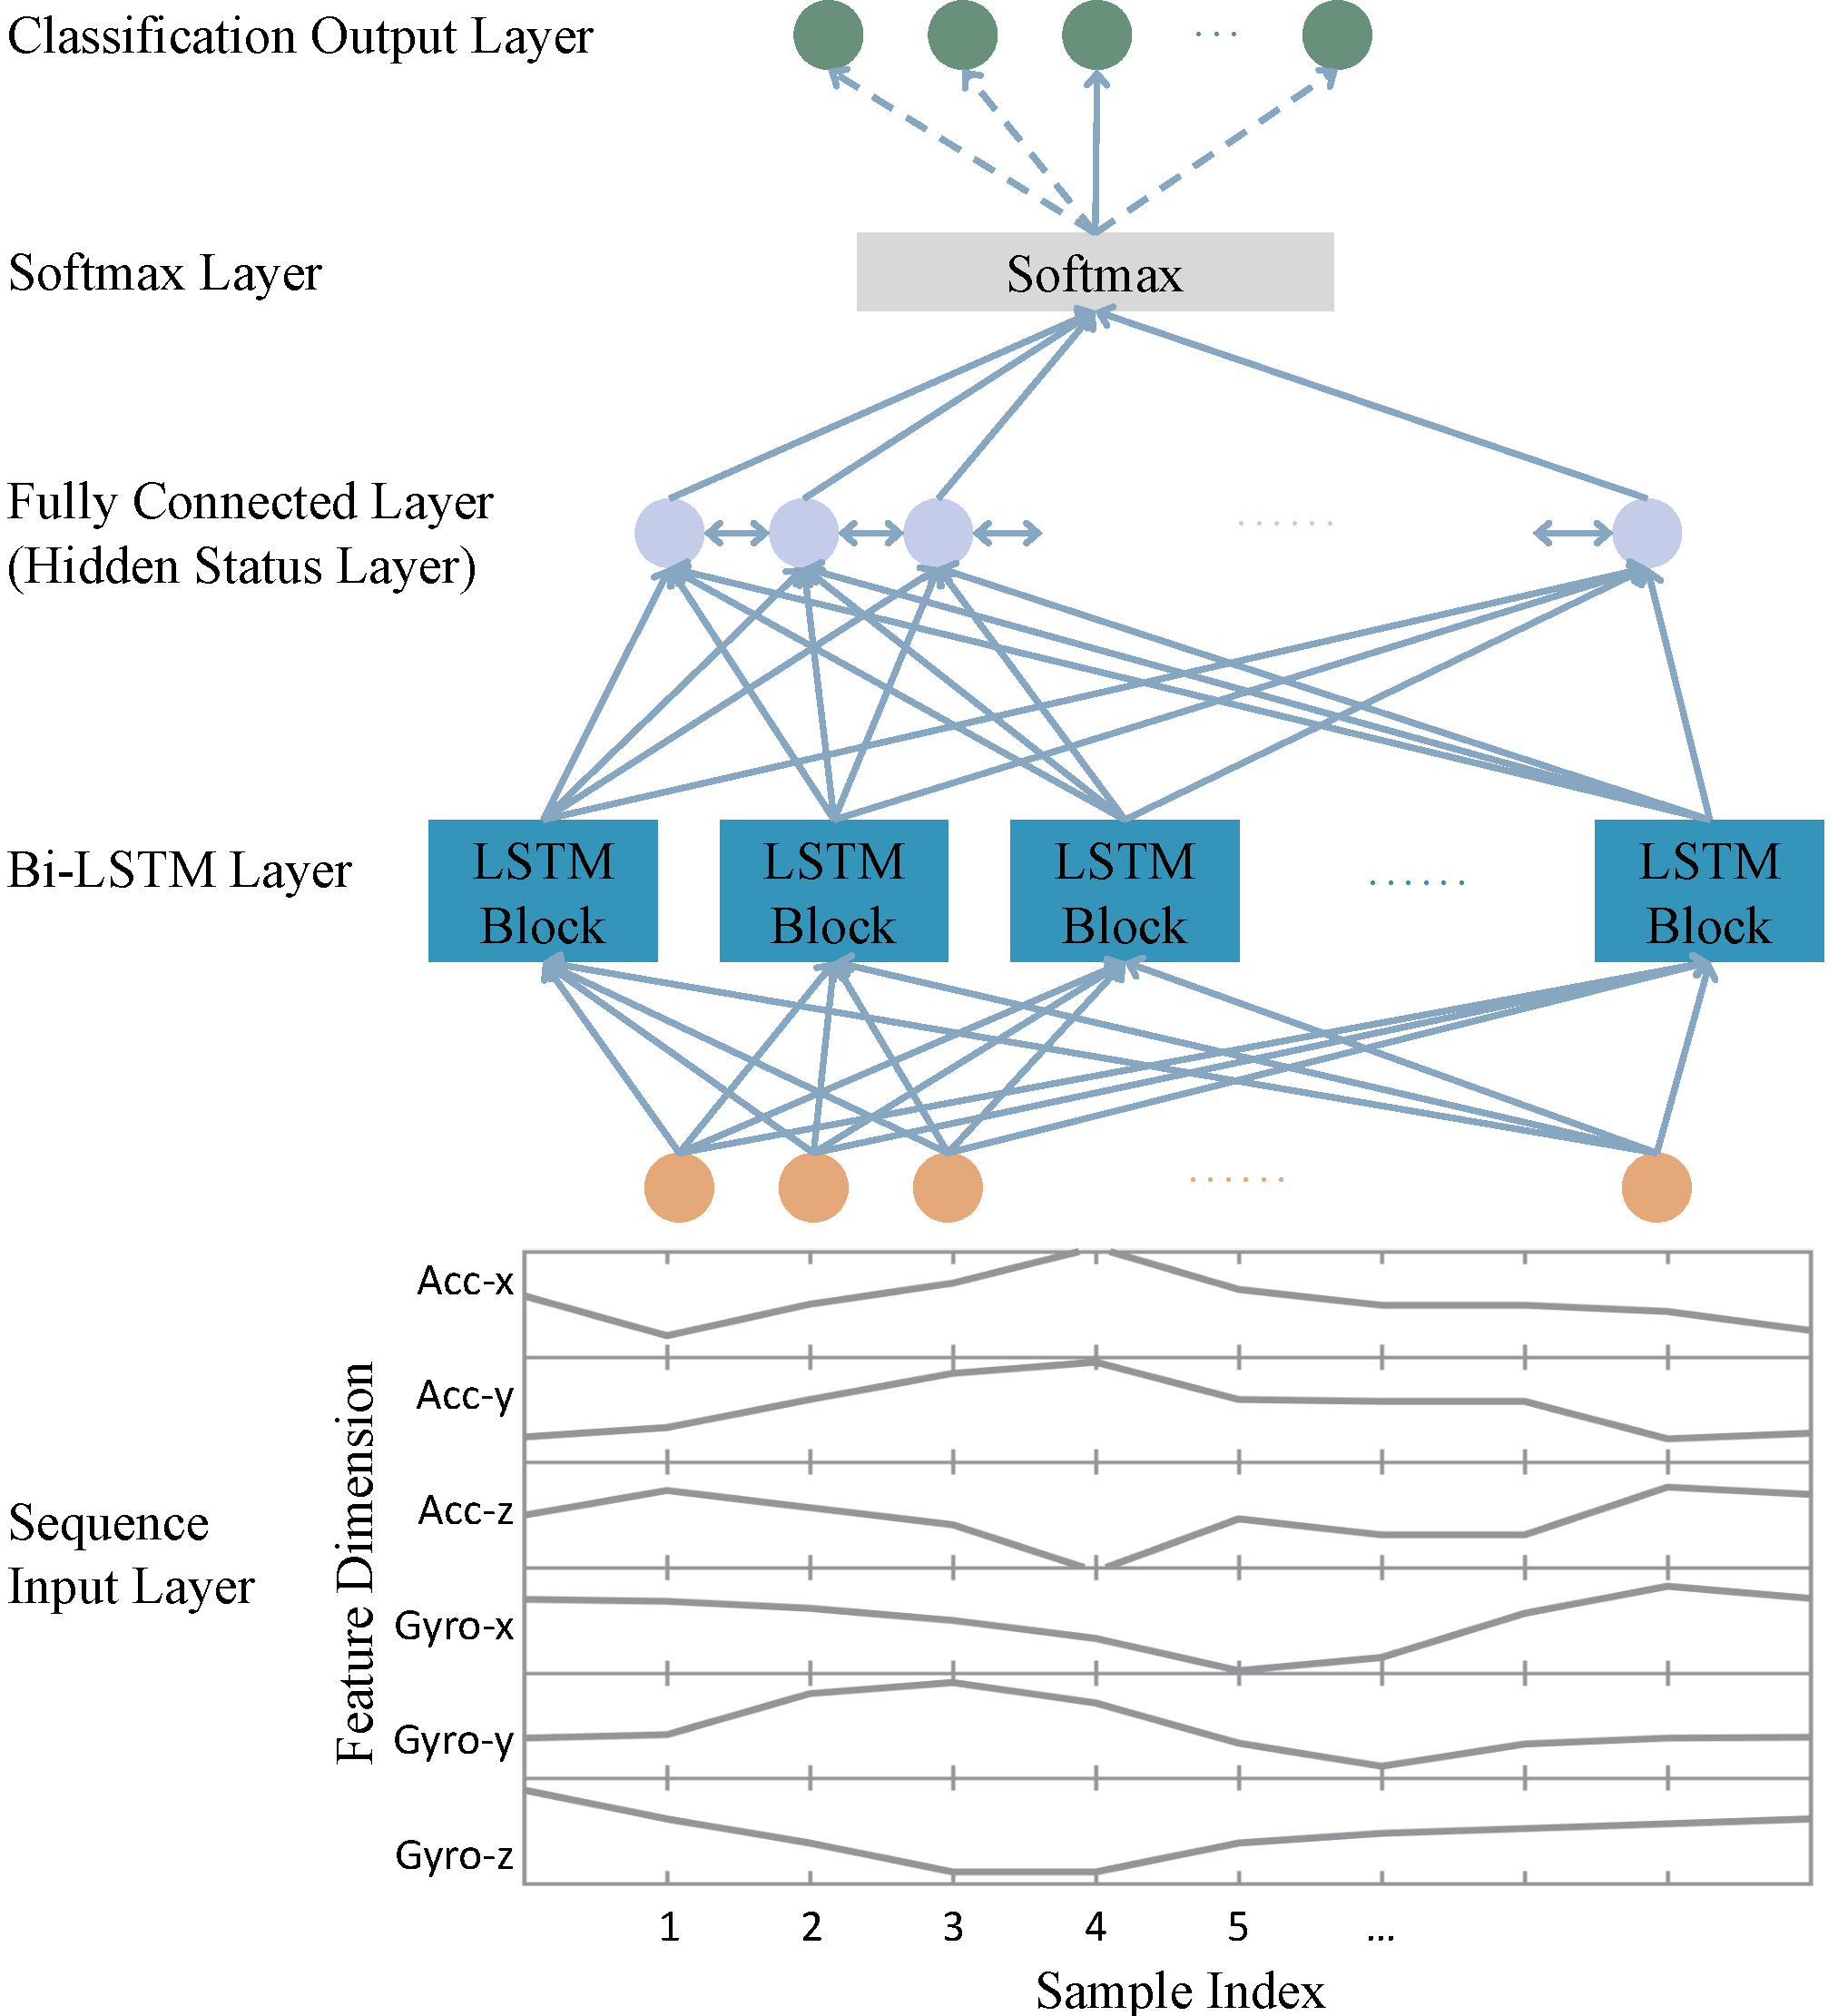
\includegraphics[width=.65\linewidth]{rnn}
	\caption{The Bidirectional Long Short-Term Memory Network (Bi-LSTM Network).}
	\label{fig:rnn}
\end{figure}


\subsection{Bi-LSTM Learing}\label{sec:LSTM}

The last stage is to use the reconstructed data to establish a Bi-directional Long Short-Term Memory (Bi-LSTM) network model, which will be used for classifying the input data later on.
%
 LSTM was first proposed by Sepp Hochreiter and J{\"u}rgen Schmidhuber in 1997 ~\cite{hochreiter1997long}. It is a special variant of  Recurrent Neural Networks (RNN), and is widely used in learning, processing, and classifying \textit{sequential } data because of 
its great property of selectively remembering patterns for long durations of time. 
%
Over the years, there have also been many variants of LSTM networks. However, based on a study in 2017, none of the variants can improve upon the standard LSTM architecture significantly~\cite{greff2017lstm}. Therefore, we still choose to implement the standard LSTM network in this work except for the bi-directional calculation. The original unidirectional LSTM network only preserves information from the inputs seen in the past. Bi-LSTM network, on the contrary, preserves information both from the past and the future. 
%
As shown in Figure~\ref{fig:rnn}, our Bi-LSTM network has five layers in total. In the sequence input layer, the input data have 6 feature dimensions, which consists of 3 accelerometer dimensions and 3 gyroscope dimensions. Then we establish an LSTM layer formed by LSTM blocks, where each block publishes its cell state to the next LSTM block. The output of the LSTM layer is sent to the fully connected hidden status layer. We set the total number of hidden units to be 100, and each hidden unit has two hidden states, one from the past and the other from the future. Then we feed the combined hidden status to a softmax function and output the classification results.





	
%

\section{Feasibility Experiments }\label{sec:experiment}

In this section, we validate the {\systemName} system and show it can eavesdrop on smartphone's built-in speakers and obtain critical information discussed in Section~\ref{sec:threat}. 


\begin{landscape}
	\centering
	\begin{table}[h]
		\caption{Comparison with Prior Works}
		\label{tab:comparison}
		\centering
		%		\resizebox{\textwidth}{!}{
		\begin{tabular}{cccccc}
			\toprule[1pt]\midrule[0.3pt]
			Work & Sensors & Setting & Main Techniques & Classification Classes & Accuracy\\
			\midrule[0.5pt]
			\multirow{4}{*}{\shortstack{~~~Gyrophone \\ ~~\cite{michalevsky2014gyrophone}}}& \multirow{4}{*}{Gyroscopes} & \multirow{4}{*}{\parbox{3cm}{\centering 10 people from TIDIGITS \\ Desktop\\ Loudspeakers}} & \multirow{4}{*}{\parbox{1.8cm}{\centering SVM\\ GMM\\ DTW}} & \multirow{2}{*}{1 to 9, Oh, Zero (11)}& Speaker-independent: 26\% \\ 
			&&&&& Speaker-dependent: 65\%\\ \cline{5-6}
			&&&&Speaker Identification& 65\%\\ \cline{5-6}
			&&&&Speaker Gender& 84\%\\
			\midrule[0.5pt]
			\multirow{3}{*}{\shortstack{~Accelword \\ ~~\cite{zhang2015accelword}}} & \multirow{3}{*}{Accelerometers }&\multirow{3}{*}{10 people} & \multirow{3}{*}{\parbox{1.8cm}{\centering Decision Tree} } & \multirow{2}{*}{\parbox{4cm}{\centering Ok Google, Hi Galaxy, Others (3)}}&\multirow{2}{*}{Speaker-dependent: 85\%}\\
			&&&&&\\ \cline{5-6}
			&&&&Speaker Identification & 86\%\\
			\midrule[0.5pt]
			\multirow{4}{*}{\shortstack{~~SpearPhone \\ ~~\cite{anand2019spearphone}}}& \multirow{4}{*}{Accelerometers} & \multirow{4}{*}{\parbox{3.5cm}{\centering 326 people from TIDIGITS \\Built-in Speakers \\in Smartphones}} & \multirow{4}{*}{\parbox{3cm}{\centering SVM with SMO\\ Logistic\\RF \\ RT}} & \multirow{2}{*}{1 to 9, Oh, Zero (11)}& \multirow{2}{*}{Speaker-dependent: 71\%} \\ 
			&&&&& \\ \cline{5-6}
			&&&&Speaker Identification& 80\%\\ \cline{5-6}
			&&&&Speaker Gender& 90\%\\
			\midrule[0.5pt]
			\multirow{4}{*}{~~~\systemName} & \multirow{4}{*}{Both} & \multirow{4}{*}{\parbox{3.5cm}{\centering 326 people from TIDIGITS \\Built-in Speakers \\in Smartphones}} & \multirow{4}{*}{\parbox{1.8cm}{\centering Compressed Sensing\\Bi-LSTM} } &1 to 9, Oh, Zero (11) &Speaker-independent: 90\%\\ \cline{5-6}
			&&&&User Activity& 81\%\\ \cline{5-6}
			&&&&Speaker Identification& 98\%\\ \cline{5-6}
			&&&&Speaker Gender& 93\%\\
			\midrule[0.3pt]\bottomrule[1pt]
		\end{tabular}
		%	}
	\end{table}
\end{landscape}

%
The main result and the comparison to prior works are summarized in Table~\ref{tab:comparison}. 


\subsection{Speech Content Learning  (Digits)}

The TIDIGITS dataset~\cite{leonard1993tidigits} has 7172 audio files of isolated digits. We use 3586 of them (3586~/~7172 =50\%) to train the dictionary. With the downsample rate $r$ set to 40, dictionary size set to ($N$=400, $K$=10), and the $p$-norm set to be the $\ell_1$-norm (absolute value), we learn an overall dictionary of size 400~$\times$~110 by concatenating each dictionary of each individual digit class. 
%
For each audio file, we play it by smartphones' built-in speakers for 30 times. Therefore, the size of the motion data is actually 30 times of the size of the sound data in the training dataset. The Bi-LSTM network is actually trained with 3586~$\times$~30=107,580 data, which are the resulted signals after preprocessing and signal reconstruction. Note that although this number seems big, each data is just 1-second data at a sampling rate of 400 Hz, and each sample is 16 bits. So the total size is 107,580~$\times$~400~$\times$~16 = 688,512,000 bits = 86.1 MB, which is indeed not big at all.


%%%TODO
%result or results
\begin{figure}[!h]
	\centering
	\includegraphics[width=.8\linewidth]{digitCFM}
	\centering
%	\resizebox{\linewidth}{!}{
		\begin{tabular}{lr}
		\toprule
		Accuracy: 90.13\% & \hspace{-.55in} Error Rate: 9.87\% \\
		Precision: 90.13\% & \hspace{-.55in} True Positive Rate (Sensitivity/Recall): 90.71\% \\
		$F_1$ Score: 0.901 & \hspace{-.55in} True Negative Rate (Specificity): 99.02\% \\
		False Negative Rate: 9.29\% & \hspace{-.55in} False Positive Rate: 0.98\% \\
		\bottomrule
	\end{tabular}

	\caption{The Confusion Matrix of the Digit Classification Result.}
	\label{fig:digitCFM}
\end{figure}
%\vspace{-.1in}
%confusion matrix
%
The test data is motion data from the remaining 3586 audio files. This data has never been seen by the Bi-LSTM network before. The classification result is shown as a confusion matrix in Figure~\ref{fig:digitCFM}. In the confusion matrix, each row of the matrix represents the instances in a predicted/output class while each column represents the instances in an actual/target class. The digit class ``zero'' has the highest classification accuracy of 98.6\%. The digit class ``eight'' has the lowest accuracy: only 70.5\% instances are classified to the correct class, while 16.2\% are classified as ``six''.
The overall accuracy of all 11 classes is 90.13\%, with a sensitivity (true positive rate) of 90.13\% and a specificity (true negative rate) of 99.02\%.


\subsection{Speech Content Learning (Commands)}\label{sec:word}
The TensorFlow Speech Commands Dataset Version 2~\cite{warden2018speech} was used for limited-vocabulary speech recognition. This dataset consists of 105,829 utterances of 35 words such as forward, house, happy, etc. A random guessing provides accuracy of 1/35 = 2.9\%, but {\systemName} could achieve 73.4\%. The accuracy is relatively lower than TIDIGITS, as TIDIGITS are professionally recorded while the commands data are crowdsourced online. Using the original 16,000 Hz audio data can only achieve accuracy of 88.2\%~\cite{warden2018speech}. {\systemName} (using 400 Hz motion data) has the correct rate of 73.4/88.2=83.2\%.

\subsection{Speaker Gender Classification and Speaker Identification}


\begin{figure}[!h]
	\begin{minipage}{\linewidth}
			\centering
		\begin{minipage}[c]{0.35\linewidth}
			
			\includegraphics[width=.9\linewidth]{digitCFMGender}
		\end{minipage}
%	\hfill
		\begin{minipage}[b]{0.49\linewidth}
			 \centering
				\begin{tabular}{r}
				\toprule
				Accuracy: 93.15\% \\ Error Rate: 6.85\% \\
				Precision: 99.19\% \\True Positive Rate : 88.28\% \\
				$F_1$ Score: 0.934 \\ True Negative Rate: 99.12\% \\
				False Negative Rate: 11.72\% \\ False Positive Rate: 0.88\% \\
				\bottomrule
			\end{tabular}
%		}
		\end{minipage}
	\end{minipage}
\caption{The Confusion Matrix of the Speaker Gender Classification Result. 
		}
%		The total number of instances of true class ``Female'' is 114$\times$11$\times$2=2508, while that of ``Male'' is 93$\times$11$\times$2=2046.}
	\label{fig:genderCFM}
\end{figure}

\begin{table}[!h]
	\caption{Statistical Analysis of the Speaker Identification Result.}
	\label{tab:idTable}
	\centering	
%	\small 
	\centering
%		\vspace{-.1in}
%	\resizebox{\linewidth}{!}{
		\begin{tabular}{lr}
		\toprule
		Accuracy: 97.56\% & \hspace{-.2in} Error Rate: 2.44\% \\
		Precision: 97.69\% & \hspace{-.2in} True Positive Rate (Sensitivity/Recall): 97.56\% \\
		$F_1$ Score: 0.976 & \hspace{-.2in} True Negative Rate (Specificity): 99.99\% \\
		False Negative Rate: 2.44\% & \hspace{-.2in} False Positive Rate: 0.01\% \\
		\bottomrule
	\end{tabular}
%}
%	\vspace{-.1in}
\end{table}

The same training and testing data are also used for gender classification and speaker identification, since the TIDIGITS audio files are labeled with gender and speaker ID. The result for gender classification is shown in Figure~\ref{fig:genderCFM}.
For speaker identification, since the number of classes is 225, we do not show the confusion matrix, but show the result of statistical analysis as in Table~\ref{tab:idTable}. The overall accuracy is 97.56\% with the sensitivity of 97.56\% and the specificity is 99.99\%.




\subsection{User Activity Classification (Sound Type)}


We also test whether the {\systemName} can classify the type of sound signals played by smartphone speakers. The dataset consists of two parts: the first is the built-in (default) alarm sounds, notification sounds and ringtones provided by the Android operating system, the other is the speech sounds from the TIMIT~\cite{garofolo1993timit} dataset where 10 sentences are spoken by each speaker.
%
In detail, we obtain 18 alarm sounds, 11 notification sounds, and 12 ringtones from \verb|/system/media/sound/| on a Google Nexus 6P smartphone with an Android 8.1 ``Oreo'' system. The speech data consist of 10 sentences from a male speaker and 10 sentences from a female speaker. We increase the atom size $N$ to 800 when building the dictionary, so that the measurement size is 800 as well, which means a piece of motion data of 800~/~400 Hz = 2~seconds. In other words, when classifying the sound type, we evaluate the motion data using a 2-second threshold, which is longer than that of classifying the digit (1~second).


\begin{figure}[ht]
	\begin{minipage}{\linewidth}
		\centering
		\begin{minipage}[c]{0.5\linewidth}			
			\includegraphics[width=.8\linewidth]{activityCFM}
		\end{minipage}
		%	\hfill
		\begin{minipage}[b]{0.49\linewidth}
			\centering
			%			\resizebox{\linewidth}{!}{
			\begin{tabular}{r}
				\toprule
				Accuracy: 80.56\% \\ Error Rate: 19.44\% \\
				Precision: 72.22\% \\ True Positive Rate: 72.49\% \\
				$F_1$ Score: 0.720\\ True Negative Rate: 94.07\% \\
				False Negative Rate: 27.51\% \\ False Positive Rate: 5.93\% \\
				\bottomrule
			\end{tabular}
			%		}
		\end{minipage}
	\end{minipage}
	
	\vspace{-.1in}
	\caption{The Confusion Matrix of the Sound Type Classification Result.}
	\label{fig:activityCFM}
	\vspace{-.1in}
\end{figure}

The result is shown in Figure~\ref{fig:activityCFM}.
 The {\systemName} system can successfully differentiate between different sound types with an overall accuracy of 80.56\%, which means attackers can know when you get up in the morning (``Alarm''), when you receive a notification (``Notification''), when you are called by others (``Ringtone''), and when the person from the other end of call starts speaking (``Ringtone'' followed by ``Speech''). Moreover, attackers can also infer activities such as watching videos or listening to audio-books (``Speech'' without ``Ringtone'' as a precursor). In other words, various sound-related user activities are not secrets to {\attackName} attackers, not to mention that motion-related activities can be monitored by motion sensors as a default.
%
Note that the average accuracy of identifying ``speech'' is 94.7\%, so the {\systemName} system can first determine whether the input belongs to ``speech'', then classify the speaker gender/identity or the digit class as mentioned above. 


The overall accuracy is much lower because of the other three classes. These classes are misclassified since alarm sounds, notification sounds and ringtones are not strictly defined. Android groups them in a generally conventional way, not by scientific methods. In fact, smartphone users may choose to use ringtones as alarms, or use alarm sounds as ringtones. Such inherent ambiguity is the main reason for the low accuracy. To further improve the accuracy, more features such as the total duration (``notification'' tends to be shorter than ``ringtones'') or the repetitive (``alarm'' tends to ring once a day) should be considered. Integrating algorithms to learn these features is a potential future work for a better design of {\systemName}.


	
%
\section{Impact Evaluation}\label{sec:impact}
In this section, we evaluate the impact of two internal parameters and three external parameters on the performance of the {\systemName} system for digit classification. 
The internal parameters control how the dictionary is learned and the external parameters control the quality of input motion data. 
%All the following experiments perform digit classification. Therefore, 
Note that a random guess results in an accuracy of 1/11 = 9.09\%.

\subsection{Impact of Training Data Size}\label{sec:impact:trainsize}
\begin{figure}[h]
	\centering
	\includegraphics[width=.5\linewidth]{trainSize}
	\vspace{-.1in}
	\caption{Impact of Training Data Size.}
	\label{fig:trainSize}
	\vspace{-.1in}
\end{figure}

The size of training data for dictionary learning is an internal parameter. In the previous section, we use 3586 audio files (50\% of full dataset) to train the dictionary. In this section, we vary the size from 660 to 1760 and show the experiment results in Figure~\ref{fig:trainSize}, which is a box and whisker plot\footnote{The ends of the box are the upper and lower quartiles (25th and 75th percentiles), the central line inside the box indicates the median, the whiskers extend to the highest and lowest accuracy values not considered outliers, and the outliers are plotted individually using the `+' symbol.}. 
We can see that the classification accuracy increases from $\sim$56\% to $\sim$78\% as the data size increases. This result is reasonable since the more data is used in training, the learned dictionary is more representative and the machine learning model is more accurate. 
%
In fact, recent researches have shown that to build a representation dictionary, the typically sufficient number of training samples grows up quasilinearly with the signal dimension, i.e., $\mathcal{O}(N\log N)$~\cite{remi2010dictionary}. In our experiment, the atom size $N$ is set to be 400, therefore, several hundred or a few thousand of training data should be enough.




\subsection{Impact of Downsampling Rate}\label{sec:impact:downrate}
\begin{figure}[h]
	\centering
	\includegraphics[width=.6\linewidth]{downsample}
	\vspace{-.1in}
	\caption{Impact of Downsampling Rate.}
	\label{fig:downsampling}
	\vspace{-.1in}
\end{figure}

The downsampling rate $r$ is the other internal parameter to study. This parameter is influenced by four frequencies: the sampling rate of smartphones' built-in speakers (48,000~Hz in Nexus 6P), the sampling rate to record human speech (20,000 Hz in TIDIGIT), the frequency range of human speech (100-4,000~Hz), and the sampling rate of motion sensors (400 Hz in Nexus 6P). 
%
We vary this rate from 5 to 50 and find that the performance of {\systemName} improves with the increase of the downsampling rate at the beginning, then the accuracy enters a relatively stable stage when $r=30$ and $r=40$. The accuracy declines if a higher downsampling rate is used ($r=50$). From Figure~\ref{fig:downsampling}, when $r \in [20, 50]$, the average accuracy is above 90\%. 
%
We do not test the cases when $r > 50$, because $50 = 20,000 Hz / 400 Hz$ is the gap between the sampling rate of training sound data and that of motion data. If we use a larger downsampling rate, the learned atoms would contain less information than the motion data, which invalidates the dictionary and contradicts with the goal of using compressed sensing to reconstruct more signal samples. 




\subsection{Impact of Training Device}\label{sec:impact:device}
We tested whether the trained LSTM network is robust across different devices. Due to time limit, only two devices are tested with the result shown in Table~\ref{tab:device}. Different devices with same model, and different devies with different model will be tested as a future work.
\begin{table}[!h]
	\caption{Statistical Analysis of the Speaker Identification Result.}
	\label{tab:device}
	\centering	
%	\small 
	\centering
%	\vspace{-.1in}
	\begin{tabular}{ccc}
		\toprule[0.5pt]
		& Nexus 6P Training& Galaxy S8 Training\\
		\midrule[0.5pt]
		Nexus 6P Testing & 90.52\% & 83.26\%\\
		Galaxy S8 Testing & 84.39\% & 90.48\% \\
		\bottomrule[0.5pt]
	\end{tabular}
%	\vspace{-.1in}
\end{table}

\subsection{Impact of Sound Volume}\label{sec:impact:volume}
\begin{figure}[!h]
	\centering
	\includegraphics[width=.9\linewidth]{volume}
	\caption{Impact of Sound Volume.}
	\label{fig:volume}
\end{figure}


In this section, we study how the sound volume affects the performance of {\systemName}. 
%
By calling the \verb|getStreamVolume(AudioManager.STREAM_MUSIC)| for the \verb|AudioManager| class, the Google Nexus 6P device supports 15 volume levels. All these volume levels are tested and the results are shown in Figure~\ref{fig:volume}. 
%
The accuracy goes up when the volume goes up. The classification accuracy is above 60\% when the volume is set to be level 10 or larger, and the accuracy goes to above 90\% when the volume is set to be the highest two levels. Even when the volume is low, the average accuracy is about 30-40\%, over 3 times higher than the random guess accuracy of 9.09\%.


\subsection{Impact of Surrounding Environment}\label{sec:impact:noise}

\begin{figure}[ht]
	\centering
	\includegraphics[width=.6\linewidth]{noise}
	\caption{Impact of Surrounding Environment.}
	\label{fig:noise}
\end{figure}

\begin{figure}[!h]
	\centering
	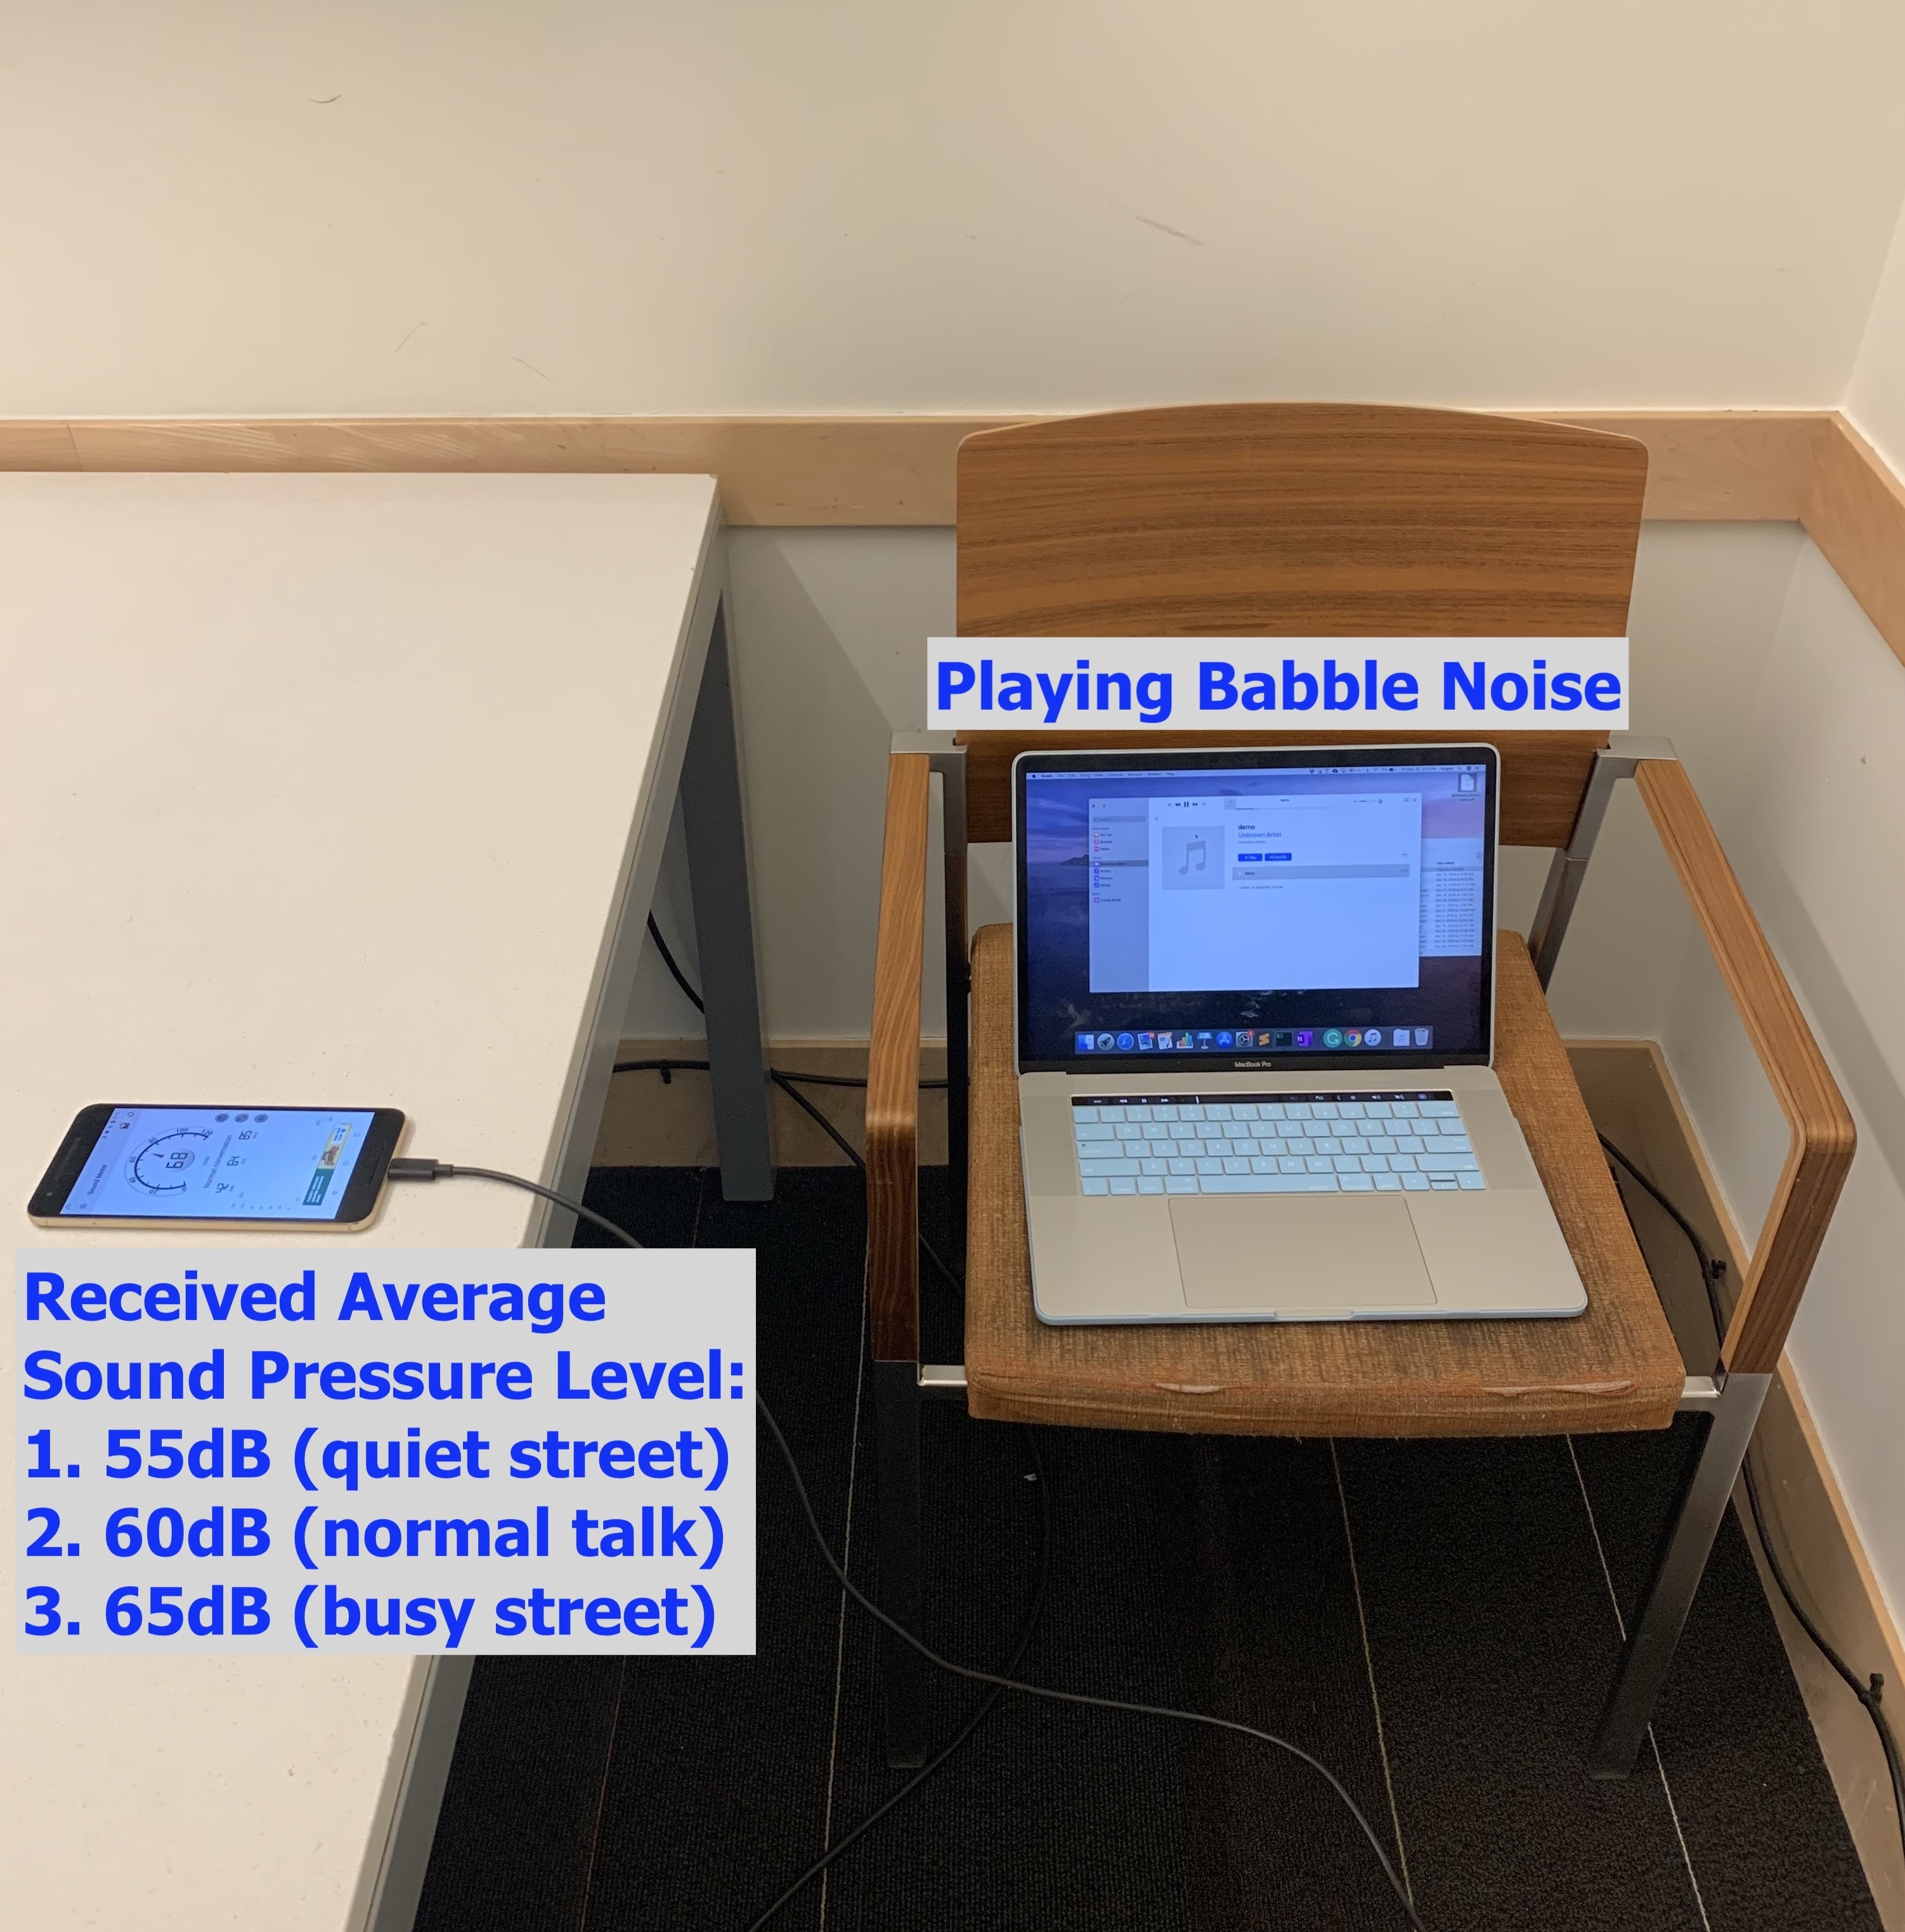
\includegraphics[width=.5\linewidth]{noisetest}
	\caption{Testing Setup.}
	\label{fig:noisetest}
\end{figure}

In this section, we test how background noises like real human talking influence the classification accuracy. When the smartphone speakers are playing sounds, a real person talks 20 cm away from the smartphone, with a similar volume. The result is shown in Figure~\ref{fig:noise}, the overall accuracy for all classes is about 60\%. Since {\systemName} still works in this experiment, it is an evidence that motion sensors are more sensitive to the built-in speakers than other sound sources that transmit signals through the air. 
%
It is worth mentioning that the performance of {\systemName} can be further improved if more training data is added. At this time, all training data are collected in a quiet environment, so directly feeding an input data from a noisy environment decreases the accuracy from 91\% to 60\%. Adding data from various environments, however, is expected to increase the robustness of the system and therefore a future research direction. 



To further test the impact of noises, we use a babble noise file and play the noise with different volumes. We control the sound pressure level received by the target phone to 55dB (quiet urban street), 60dB (normal conversation), and 65 dB (busy street). The results are shown in Figure ~\ref{fig:noisetestresult}.

\begin{landscape}
	\begin{figure}[!h]
		
		\begin{minipage}[c]{.33\linewidth}
			\centering
			\includegraphics[width=\textwidth]{digitDB55CFM}
			\tiny
			\begin{tabular}{lr}
				\toprule
				Accuracy: 88.87\% & \hspace{-.00in} Error Rate: 11.13\% \\
				Precision: 88.87\% & \hspace{-.00in} True Positive Rate: 89.20\% \\
				$F_1$ Score: 0.889 & \hspace{-.00in} True Negative Rate: 98.89\% \\
				False Negative: 10.80\% & \hspace{-.00in} False Positive Rate: 1.11\% \\
				\bottomrule
			\end{tabular}
			\subcaption{Quiet Street (55 dB noise)}
		\end{minipage}
		\begin{minipage}[c]{.33\linewidth}
			\centering
			\includegraphics[width=\textwidth]{digitDB60CFM}
			\tiny
			\begin{tabular}{lr}
				\toprule
				Accuracy: 85.48\% & \hspace{-.00in} Error Rate: 14.52\% \\
				Precision: 85.49\% & \hspace{-.00in} True Positive Rate: 86.16\% \\
				$F_1$ Score: 0.855 & \hspace{-.00in} True Negative Rate: 98.55\% \\
				False Negative: 13.84\% & \hspace{-.00in} False Positive Rate: 1.45\% \\
				\bottomrule
			\end{tabular}
			\subcaption{Normal Conversation (60 dB noise)}
		\end{minipage}
		\begin{minipage}[c]{.33\linewidth}
			\centering
			\includegraphics[width=\textwidth]{digitDB65CFM}
			\tiny
			\begin{tabular}{lr}
				\toprule
				Accuracy: 77.50\% & \hspace{-.00in} Error Rate: 22.50\% \\
				Precision: 77.47\% & \hspace{-.00in} True Positive Rate: 77.61\% \\
				$F_1$ Score: 0.773 & \hspace{-.00in} True Negative Rate: 97.76\% \\
				False Negative: 22.39\% & \hspace{-.00in} False Positive Rate: 2.24\% \\
				\bottomrule
			\end{tabular}
		\subcaption{Noisy Street (65 dB noise)}
		\end{minipage}
		\caption[Impact of Surrounding Environments.]{The Impact of Surrounding Environments: Quiet Street, Normal Conversation, and Noisy Street. Note that the decibel values are the average sound pressure levels received by the smartphone. }
		\label{fig:noisetestresult}
	\end{figure}
\end{landscape}


\subsection{Impact of User Mobility}\label{sec:impact:move}
All previous experiments are conducted when the smartphone is placed on a desk, without being touched or moved during the data collection stage. As illustrated in Figure~\ref{fig:spyphonepreprocess}, user movements are regarded as noises. Fortunately, since user movement is very slow and is unlikely to generate signals as high as 50 Hz. Thus, we can apply a high pass filter to mitigate the noise. In Figure~\ref{fig:newspec}, we see noises are removed after the filter. In this section, we validate the performance of {\systemName} with the presence of user mobility. 

We conduct two experiments: the walking scenario and the driving scenario. The users put the phone in their pockets while playing the sounds using the speakers. The results are shown in Figure~\ref{fig: walkanddrive}. The accuracy for the walking scenario is 83.94\% and that of driving scenario is 73.34\%. The accuracy of the driving scenario is relatively lower because of frequencies of the noises are relatively higher and thus close to the aliasing of human speech.

Moreover, we conduct an experiment in the extreme case that the user holds the phone in the hand and keeps moving it. The results are plotted in Figure~\ref{fig:move}, the average accuracy can still achieve 45\%.

\begin{figure}[!h]
	\centering
	\includegraphics[width=.6\linewidth]{move}
	\caption{Impact of User Mobility.}
	\label{fig:move}
\end{figure}


\begin{landscape}
	\begin{figure}[!h]
		\centering
		\begin{minipage}[c]{.48\linewidth}
			\centering
			\includegraphics[width=\textwidth]{digitWalkCFM}
			\begin{tabular}{lr}
				\toprule
				Accuracy: 83.94\% & \hspace{-.00in} Error Rate: 16.06\% \\
				Precision: 83.94\% & \hspace{-.00in} True Positive Rate: 84.05\% \\
				$F_1$ Score: 0.839 & \hspace{-.00in} True Negative Rate: 98.39\% \\
				False Negative Rate: 15.95\% & \hspace{-.00in} False Positive Rate: 1.61\% \\
				\bottomrule
			\end{tabular}
		\end{minipage}
		\begin{minipage}[c]{.48\linewidth}
			\centering
			\includegraphics[width=\textwidth]{digitDriveCFM}
			\begin{tabular}{lr}
				\toprule
				Accuracy: 73.34\% & \hspace{-.00in} Error Rate: 26.66\% \\
				Precision: 73.34\% & \hspace{-.00in} True Positive Rate: 73.59\% \\
				$F_1$ Score: 0.733 & \hspace{-.00in} True Negative Rate: 97.34\% \\
				False Negative Rate: 26.41\% & \hspace{-.00in} False Positive Rate: 2.66\% \\
				\bottomrule
			\end{tabular}
		\end{minipage}
		\caption[Accuracy in the walking (left) and driving (right) scenario.]{Accuracy in the walking (left) and driving (right) scenario. The machine learning model trained in the stable environment is directly used to predict the testing data collected when user is walking or driving.}
		\label{fig: walkanddrive}
	\end{figure}
\end{landscape}




%


\section{Defenses}
%To defend against an attacker that has only user-level access to the device (an application or a web- site), it might be enough to apply low-pass filtering to the raw samples provided by the gyroscope. Judging by the sampling rate available for Blink and WebKit based browsers, it is enough to pass frequencies in the range 0 – 20 Hz. If this rate is enough for most of the applications, the filtering can be done by the driver or the OS, subvert- ing any attempt to eavesdrop on higher frequencies that reveal information about surrounding sounds. In case a certain application requires an unusually high sampling rate, it should appear in the list of permissions requested by that application, or require an explicit authorization by the user. To defend against attackers who gain root access, this kind of filtering should be performed at the hardware level, not course, it imposes a able to applications.
%Another possible masking. It can be possibly on the case
%being subject to configuration. Of restriction on the sample rate avail-
%solution is some kind of acoustic applied around the sensor only, or
%of the mobile device.

%%TODO take defense?
To defend against the {\attackName} attack, the smartphone user can adopt the hardware-based defenses or the software-based defenses if supported by the smartphone's operating systems.
%\vspace{-.1in}
\subsection{Hardware-based Defenses}
%\textbf{Hardware-based Defenses: }
The easiest way to defend the {\attackName} attack is to not use smartphone's built-in speakers. Instead, a user can use \textit{headphones} or other wireless connected loudspeakers. As long as there is no direct contact between the speakers and the motion sensors, the attack is defended~\cite{anand2018speechless}. In fact, as shown in Section~\ref{sec:impact:volume}, with lower volume setting, the {\attackName} attack can also be largely impeded. Though such hardware-based defenses may cause inconvenience to the user, their security and privacy can be protected.
%Loudspeaker not loud
%newly-released OSchoose to keep the OS version, do not or can not upgrade to the
%Use headphones
%\vspace{-.1in}
\subsection{Software-based Defenses}
%\textbf{Software-based Defenses: }
The software-based defenses are better sensor management by smartphones' operating systems (OS). For example, the OS should treat the permissions to motion sensors as dangerous permissions and require users to grant permissions at installation time. Moreover, the OS should keep monitoring the sensor usage such as when the sensors are used, whether they are used in background, and what sampling rate is required by the application. 


Though there has been some research in designing better sensor management systems~\cite{sikder20176thsense}, the {\attackName} attack may still be a big threat for at least three years. This is because the smartphone users may not or can not upgrade to the 
newly-released OS in a timely manner. 
%For example, more than half the Android devices are still using OS as old as Android Nougat, which was released in 2016\footnote{\scriptsize \url{https://developer.android.com/about/dashboards}}. 
%
Indeed, by the end of May 7, 2019, more than half the Android devices are still using OS released three years ago~\footnote{More than half the Android devices are still using OS as old as Android Nougat, which was released in 2016 according to Android Dashboards (\url{https://developer.android.com/about/dashboards})}. Therefore, three years later, there is a large chance that more than half the devices are still using the OS released so far. Since current Android OS cannot defend the SpyPhone system, those devices are vulnerable to the Man-in-the-Phone attack. However, if smartphone users know the importance of the update and cares about their security and privacy, the adoption speed may increase. Note that there is a huge lag between Google and the manufacturers such as Samsung and Huawei. Even Google release the security updates quickly enough, the manufacturer may release them too late.

%~\cite{onlinedashboards}.
%

\section{Related Work}

\subsection{Inferring  Information From Smartphone Motion Sensors}
%Modern mobile devices such as smartphones are equipped with more and more powerful motion sensors(i.e., accelerometer, gyroscope).
%
In recent years, much attention has been paid to inferring private information  through motion sensors in the literature.
%
A typical side-channel attack is keystrokes inference on smartphones through motion sensors~\cite{owusu2012accessory,miluzzo2012tapprints}. 
%
The general idea of these attacks is that when typing on different locations on a screen, the keystrokes cause distinct vibrations or rotations. 
%
In addition, Wang \emph{et al.}~\cite{wang2015mole} proposed to track the movement of the wrist to infer what the user has typed.
% 
Similarly, a practical attack has been shown in~\cite{wang2016friend}, which infers a user’s personal PIN sequence by exploiting wearable devices.
%
The feasibility of inferring user’s location information using motion sensors instead of GPS data has been shown in~\cite{liang2017location,han2012accomplice}.
%
Bojinov \emph{et al.}~\cite{bojinov2014mobile} demonstrated that motion sensors can be used as device fingerprint to uniquely identify a device. 
%
This motion sensor-based device fingerprint was further utilized by~\cite{das2016tracking} to track a user across multiple visits to websites.
%
In~\cite{lee2018inferring}, Lee \emph{et al.} proposed to use motion sensors to infer users' handwritten patterns.
%
Huang \emph{et al.}~\cite{huang2018breathlive} implemented a reliable liveness detection system called Breathlive, which is based on the inherent correlation between sounds and chest motion caused by deep breathing.
%
Roy \emph{et al.}~\cite{roy2015ripple} demonstrated the possibility of communication through motion sensors by modulating the vibration motor and decoding through accelerometers. 
%
Recent works on activity recognition using motion sensors are presented in~\cite{shoaib2015survey,wang2019deep}.
%
In addition, a detailed survey of works on sensor-based threats for smart devices can be found in~\cite{sikder2018survey, crager2017information}.
%===========================================================
%
Note that we only list related works using smartphone motion sensors, but not works using standalone sensors. This is because smartphone motion sensors can only report readings at a low frequency, but standalone accelerometers or gyroscopes can record signals with frequencies as high as 10 KHz. Some special models of piezoelectric accelerometers can even measure 1~MHz signals.
\subsection{Eavesdropping Sound Signals By Non-Acoustic Sensors}
Recent studies have shown that sound signals can be eavesdropped through non-acoustic sensors instead of microphones.
%
Among these side-channel attacks, MEMS motion sensors are widely used since motion sensors are prone to acoustic signals.
%
Michalevsky \emph{et al.}~\cite{michalevsky2014gyrophone} found that the MEMS gyro sensors are able to pick up air vibrations from sound. 
%
They proposed GyroPhone, a new threat which uses  gyroscope on smartphone to intercept human speech.  
%
Zhang \emph{et al.}~\cite{zhang2015accelword} proposed to utilize accelerometer  for hotword detection to reduce power consumption.
%
In addition, Anand \emph{et al.}~\cite{anand2018speechless} also demonstrated that it is possible to eavesdrop speech signals in certain scenarios by using inertial sensors in a smartphone. 
%
Han \emph{et al.}~\cite{han2017pitchln} proposed to combine multiple signals from non-acoustic sensors to create a higher sample rate signal for speech reconstruction.
%
Hawley \emph{et al.}~\cite{hawley2018visualizing} proposed to use sensors on smartphone to visualize the properties of sound directivity, interference and other acoustical phenomena. 
%
Recently, other techniques have been proposed to eavesdrop sound signals besides motion sensors.
%
Roy \emph{et al.}~\cite{roy2016listening} have shown that the vibration motor  can be used as microphone since the vibrating mass inside the motor responds to air vibrations from nearby sounds.
%
Davis \emph{et al.}~\cite{davis2014visual} used a high speed camera to retrieve digital audio by capturing the vibration of objects near the sound source.
%
Similarly, Fuse \emph{et al.}~\cite{fuse2018sound} found that a better sound can be obtained by trying to recover the sound based on the vibration direction of the object.
%
Kwong \emph{et al.}~\cite{kwonghard} demonstrated that the mechanical components in magnetic hard disk drives can be used to extract and parse human speech with sufficient precision. 


%
%\section{Related Work}
%
%Eaves sound signal using non- acoustic sensor;;
%
%
%Information using motion sensor on smartphone
%acce -> keytroke, pin, ...
%
%
%used to measure angular rotation, across x, y, and z axes.
%Motion sensors have been shown prone to acoustic noise particularly at high frequency and power level in [12], [13], [14], which showed that MEMS gyroscopes are susceptible to high power, high frequency noise that contains frequency components in proximity of the resonating frequency of the gyroscope’s proof mass. This concept of work was further utilized by Son et al. [15] to interfere with the flight control system of a drone using intentional sounds that were produced by a Bluetooth speaker attached to the drones with a sound 
%
%but On smartphones, ~\cite{michalevsky2014gyrophone} are first.
%
%\subsection{Eavasdrop sound signals on smartphones}
%
%visual
%vibration sensor
%
%
%
%
%\subsection{Eavasdrop sound signals using sensors other than microphone}
%
%
%Security of sensor-equipped devices
%
%
%Sensor-based threats [76] on mobile devices have be- come more prevalent than before with the use of dif- ferent sensors in smartphones such as user’s location, keystroke information, etc. Different works [73] have in- vestigated the possibility of these threats and presented different potential threats in recent years. One of the most common threats is keystroke inference in smart- phones. Smartphones use on-screen QWERTY keyboard which has specific position for each button. When a user types in this keyboard, values in smartphone’s motion sensor (i.e., accelerometer and gyroscope) change ac- cordingly [16]. As different keystrokes yield different, but specific values in motion sensors, typing informa- tion on smartphones can be inferred from an unautho- rized sensor such as motion sensor data or motion sen- sor data patterns collected either in the device or from a nearby device can be used to extract users’ input in smartphones [9, 66, 52]. The motion sensor data can be analyzed using different techniques (e.g., machine learning, frequency domain analysis, shared-memory ac- cess, etc.) to improve the accuracy of inference tech- niques such as [12, 53, 81, 46, 58, 47]. Another form of
%keystroke inference threat can be performed by observ- ing only gyroscope data. Smartphones have a feature of creating vibrations while a user types on the touch- pad. The gyroscope is sensitive to this vibrational force and it can be used to distinguish different inputs given by the users on the touchpad [51, 15, 44]. Recently, ICS-CERT also issued an alert for accelerometer-based attacks that can deactivate any device by matching vi- bration frequency of the accelerometer [2, 1, 70]. Light sensor readings also change while a user types on the smartphone; hence, the user input in a smartphone can be inferred by differentiating the light sensor data in nor- mal and typing modes [71]. The light sensor can also be used as a medium to transfer malicious code and trigger message to activate malware [28, 76]. The audio sen- sor of a smartphone can be exploited to launch different malicious attacks (e.g., information leakage, eavesdrop- ping, etc.) on the device. Attackers can infer keystrokes by recording tap noises on touchpad [24], record conver- sation of users [63], transfer malicious code to the device [73, 76], or even replicate voice commands used in voice- enabled different Apps like Siri, Google Voice Search, etc. [21, 39]. Modern smartphone cameras can be used to covertly capture screenshot or video and to infer infor- mation about surroundings or user activities [68, 43, 67]. GPS of a smartphone can be exploited to perform a false data injection attack on smartphones and infer the loca- tion of a specific device [75, 19].
%
%
%
%%\begin{landscape}
	\SingleSpacing
	
	\begin{longtable}{p{3cm}p{6cm}p{6cm}ccc} %p{1.5cm}
		\caption{Related Work on Liveness Detection}
		\label{tab:liveness}
		\\
		
		\toprule
				Authors & Method & Shortcomming & Accuracy & \shortstack{No Extra \\ Devices} &  \shortstack{No Cumbersome \\ User Interaction}  \\
	%			& No User-specific Training\\
		\midrule
		
		\endfirsthead
		
		\normalfont\tablename~\thetable{}~Continued\\
		\toprule
				Authors & Method & Shortcomming & Accuracy & \shortstack{No Extra \\ Devices} &  \shortstack{No Cumbersome \\ User Interaction}  \\
	%			& No User-specific Training\\
		\midrule
		
		\endhead
		
		\bottomrule		
		\endfoot
		
		\endlastfoot
			Girija Chetty and Michael Wagner~\cite{chetty2004automated} & Detecting lip movements using cameras. & Inherits shortcomings of face authentication and introduces high computational overhead. & 99\% & \xmark & \cmark \\
%			& \xmark\\
			Poss et al.~\cite{poss2008biometric} & Using neural tree networks to determine unique aspects of utterances and Hidden Markov Models to classify them. & The accuracy is unkown. & - & \cmark & \cmark 
			\\
%			& \xmark \\
			Wei Shang and Maryhelen Stevenson~\cite{shang2010score} & Testing whether an incoming recording shares the same originating utterance as any of N stored recordings. & Performance is largely based on the pre-stored recordings. & 88.1\%/93.2\% & \cmark & \cmark 
			\\
%			& \xmark \\
			Jes{\'u}s Villalba and Eduardo Lleida~\cite{villalba2011detecting} & Detecting noises and spectrum changes caused by far-field microphone and loudspeakers. & Limits the replay attackers to use far-field microphones. & 91\%-100\% & \cmark & \cmark \\
%			& \cmark \\
			Wang et al.~\cite{wang2011channel} & Detecting channel pattern noise caused by microphone and loudspeakers. & Limits the replay attackers to use low-quality microphones. & 97\% & \cmark & \cmark 
			\\
%			& \cmark \\			
			Aley-Raz et al.~\cite{aley2013device}  & Integrating intra-session voice variation to Nuance VocalPassword~\cite{onlinenuance}. & Requires the user to cumbersomely repeat prompted sentences. & - & \cmark & \xmark 
			\\
%			& \cmark \\
			Zhang et al.~\cite{zhang2016voicelive} & \textbf{VoiceLive}: Measuring the time-difference-of-arrival changes of a sequence of phoneme sounds to the two microphones of the phone. & Requires at least two high-quality microphones in one smartphone. & 99\% & \cmark & \cmark 
			\\
%			& \xmark \\
			Chen et al.~\cite{chen2017you} & Detecting the magnetic field emitted from loudspeakers. & Requires the user to move the smartphone with the predefined trajectory around the sound source. & 100\% & \cmark & \xmark 
			\\
%			& \cmark \\			
			Zhang et al. ~\cite{zhang2017hearing} & \textbf{VoiceGesture}: Leverages Dopler shifts in signals caused by users' articulatory gestures when speaking. & Requires high quality microphones and needs a longer computation time. & 99\% & \cmark & \cmark
			\\
%			 & \xmark \\
			Feng et al.~\cite{feng2017continuous}  & \textbf{VAuth}: Utilizing the instantaneous consistency of the entire signal from the accelerometer and the microphone. & Requires the user to wear high-sampling-rate accelerometers on the facial, throat, or sternum areas. & 97\% & \xmark & \cmark 
			\\
%			& \cmark \\
			Huang et al.~\cite{huang2018breathlive}  & \textbf{BreathLive}: Utilizing chest movement when making deep breaths & The sound is deep breath sound instead of human speech; Stethoscope is needed. & 91\%/94\%/96\% & \xmark & \cmark 
			\\
%			& \xmark \\
			Ment et al.~\cite{meng2018wivo} & \textbf{WiVo}: Using channal state information (CSI) from WiFi signals to detect mouth movement  &  Requires WiFi antennas to collect the CSI info; the distance between antennas and human is short (20cm). & 99\% & \xmark & \cmark
 \\
\bottomrule

\end{longtable}

\end{landscape}

%\begin{landscape}	
%	\begin{table}
%		\centering
%%		\renewcommand{\arraystretch}{1.5}
%%		\caption{Related Work on Liveness Detection}
%%		\label{tab:liveness}
%		\footnotesize
%		\begin{tabular}{p{2.5cm}p{0.5cm}p{4.5cm}p{4.5cm}ccc} %p{1.5cm}
%			\toprule\specialrule{0.5pt}{1.5pt}{\belowrulesep}
%			Authors & Year & Method & Shortcomming & Accuracy & \shortstack{No Extra \\ Devices} &  \shortstack{No Cumbersome \\ User Interaction}  \\
%%			& No User-specific Training\\
%			\midrule
%			Girija Chetty and Michael Wagner~\cite{chetty2004automated} & 2004 & Detecting lip movements using cameras. & Inherits shortcomings of face authentication and introduces high computational overhead. & 99\% & \xmark & \cmark \\
%%			& \xmark\\
%			Poss et al.~\cite{poss2008biometric} & 2008 & Using neural tree networks to determine unique aspects of utterances and Hidden Markov Models to classify them. & The accuracy is unkown. & - & \cmark & \cmark 
%			\\
%%			& \xmark \\
%			Wei Shang and Maryhelen Stevenson~\cite{shang2010score} & 2010 & Testing whether an incoming recording shares the same originating utterance as any of N stored recordings. & Performance is largely based on the pre-stored recordings. & 88.1\%/93.2\% & \cmark & \cmark 
%			\\
%%			& \xmark \\
%			Jes{\'u}s Villalba and Eduardo Lleida~\cite{villalba2011detecting} & 2011 & Detecting noises and spectrum changes caused by far-field microphone and loudspeakers. & Limits the replay attackers to use far-field microphones. & 91\%-100\% & \cmark & \cmark \\
%%			& \cmark \\
%			Wang et al.~\cite{wang2011channel} & 2011 & Detecting channel pattern noise caused by microphone and loudspeakers. & Limits the replay attackers to use low-quality microphones. & 97\% & \cmark & \cmark 
%			\\
%%			& \cmark \\			
%			Aley-Raz et al.~\cite{aley2013device}  & 2013 & Integrating intra-session voice variation to Nuance VocalPassword~\cite{onlinenuance}. & Requires the user to cumbersomely repeat prompted sentences. & - & \cmark & \xmark 
%			\\
%%			& \cmark \\
%			Zhang et al.~\cite{zhang2016voicelive} & 2016 & \textbf{VoiceLive}: Measuring the time-difference-of-arrival changes of a sequence of phoneme sounds to the two microphones of the phone. & Requires at least two high-quality microphones in one smartphone. & 99\% & \cmark & \cmark 
%			\\
%%			& \xmark \\
%			Chen et al.~\cite{chen2017you} & 2017 & Detecting the magnetic field emitted from loudspeakers. & Requires the user to move the smartphone with the predefined trajectory around the sound source. & 100\% & \cmark & \xmark 
%			\\
%%			& \cmark \\			
%			Zhang et al.~\cite{zhang2017hearing} & 2017 & \textbf{VoiceGesture}: Leverages Dopler shifts in signals caused by users' articulatory gestures when speaking. & Requires high quality microphones and needs a longer computation time. & 99\% & \cmark & \cmark
%			\\
%%			 & \xmark \\
%			Feng et al.~\cite{feng2017continuous}  & 2017 & \textbf{VAuth}: Utilizing the instantaneous consistency of the entire signal from the accelerometer and the microphone. & Requires the user to wear high-sampling-rate accelerometers on the facial, throat, or sternum areas. & 97\% & \xmark & \cmark 
%			\\
%%			& \cmark \\
%			Huang et al.~\cite{huang2018breathlive}  & 2018 & \textbf{BreathLive}: Utilizing chest movement when making deep breaths & The sound is deep breath sound instead of human speech; Stethoscope is needed. & 91\%/94\%/96\% & \xmark & \cmark 
%			\\
%%			& \xmark \\
%			Ment et al.~\cite{meng2018wivo} & 2018 & \textbf{WiVo}: Using channal state information (CSI) from WiFi signals to detect mouth movement  &  Requires WiFi antennas to collect the CSI info; the distance between antennas and human is short (20cm). & 99\% & \xmark & \cmark
%			\\
%		\specialrule{0.5pt}{\aboverulesep}{1.5pt}\bottomrule
%		\end{tabular}
%	\end{table}
%\end{landscape}

%Shang et al.~\cite{shang2010score} propose to compare an input voice sample with stored instances of past accesses to detect the voice samples have been seen before by the authentication system. This method, however, cannot work if the attacker records the voice samples during a non-authentication time point. Villalba et al. and Wang et al. suggest that the additional channel noises introduced by the recording and loudspeaker can be used for attack detection~\cite{villalba2011detecting,wang2011channel}.
%These approaches however have limited effec- tiveness in practice. For example, the false acceptance rates of these approaches are as high as 17\%. Chetty and Wagner propose to use video camera to extract lip movements for liveness verification~\cite{chetty2004automated}, whereas Poss et al. combine the techniques of a neural tree network and Hidden Markov Models to improve authentication accuracy~\cite{poss2008biometric}.
%Aley-Raz et al.~\cite{aley2013device} develop a liveness detection system based on ``Intra-session voice variation'', which is integrated into Nuance VocalPassword~\cite{onlinenuance}. In addition to a user-chosen passphrase, it requires a user to repeat one or more random sentences prompted by the system for liveness detection. Such a method however increases the op- eration overhead of the user and is cumbersome due to an explicit user cooperation is required besides the standard authentication process. 
%
%More recently, Chen et al.~\cite{chen2017you} develop a smartphone based liveness detection system by measuring the magnetic field emit- ted from loudspeakers. It however requires the user to speak the passphrase while moving the smartphone with predefined trajectory around the sound source. Moreover, Zhang et al.~\cite{zhang2016voicelive} propose a smarthphone based solution, which measures the time-difference-of-arrival (TDoA) changes of a sequence of phoneme sounds to the two microphones of the phone when a user speaks a passphrase for liveness detection. However, it requires at least two high-accuracy microphones in one smartphone. Zhang et al.~\cite{zhang2017hearing} then propose VoiceGuesture, which leverages a user’s articulatory gestures when speaking a passphrase for liveness detection. However, the calculation overhead is high.
%Feng et al.~\cite{feng2017continuous} present VAuth,  which utilizes the instantaneous consistency of the entire signal from the accelerometer and the microphone.  However, it requires the user to wear a security-assisting device on the facial, throat, or sternum areas. 
%Huang et al.~\cite{huang2018breathlive} present BreathLive, which utilize the inherent correlation between sounds and chest motion caused by deep breathing to realize a reliable liveness detection system. However, it requires special gyroscope and stethoscope. Since it utilizes deep breathing, the sound period is very long (4 sec. for one deep breathing).
%
%In conclusion, the aforementioned approaches either require cumbersome user interaction, or require extra electronic devices, or require long recording time or processing time. Building a good liveness detection component is still an open problem.
%
%Privacy leakage through sensors.
%
%
%information leaks using motion sensors.
%
%
%WALNUT:
%
%Information Leakage
%Information leakage from physical properties, or side-channels, of computing systems are also relevant to analog cybersecurity. Recent studies show that gyroscopes and accelerometers can leak personal information [12]–[13][14][15][16]. Michalevsky et al. show that gyroscopes in smart-phones can be used as a microphone to eavesdrop on conversations [16]. Marquardt et al. demonstrate that smart-phone accelerometers leak enough information to infer keystrokes from a nearby keyboard [12]. Similarly, Owusu and Aviv show smart-phone accelerometer information leakage can be leveraged to infer user touchscreen gestures and key presses to leak passwords and PIN codes to unlock phones [14], [15]. Dey et al. found that process variation in accelerometers yields a unique fingerprint that can uniquely identify a device [13]. These efforts are a reminder that physical attacks on analog sensors render securing data integrity, authentication, and confidentiality between sensors and microprocessors challenging.
%
%~\cite{aaaGoogleSearch,anand2018speechless,crager2017information,davis2014visual,han2017pitchln,jafari2011fast,jafaridictionary,khalifa2016feasibility,khan2018firearm,maruri2018v,matic2012speech,michalevsky2014gyrophone,michalevsky2014gyrophone,roy2016listening,sikder20176thsense,song2016my,wei2015acoustic,welsh2017smartphone,zhang2015accelword}
%
\section{conclusion}

Self demodulation and acoustic attenuation can be used to build {\shortname}, a spoof-proof voice authentication system. When a user speaks with the smartphone placed on his throat, his voice not only influences the microphone readings, but also affects the accelerometer and gyroscopes. By adopting a sequence-to-sequence long short-term memory network, syllable separation, and majority voting, \shortname~can defend against 3 different types of attacks with 90.43\% defend rate and a 92.98\% acceptance rate for legitimate users.




\begin{landscape}
	\begin{figure}[h]
		\centering
		\begin{minipage}{.48\linewidth}
			\includegraphics[width=\linewidth]{movoUserBefore}
			\subcaption{Without Majority Voting}\label{fig:usermata}
			\vspace{.05in}
		\end{minipage}
		\begin{minipage}{.48\linewidth}
			\includegraphics[width=\linewidth]{movoUserAfter}
			\subcaption{With Majority Voting}\label{fig:usermatb}
			\vspace{.05in}
		\end{minipage}
		\caption{Confusion Matrix of Matching Motion Data to Different Users.}
		\label{fig:usermat}
	\end{figure}
\end{landscape}

%========================================
%                            Chapter                            
%======================================== 
\chapter{{\uu}: Smartphone Authentication \protect \\ Using Gestures in the Air}

In this chapter, we propose a new authentication method for smartphones. During the authentication period, the smartphone's built-in speaker transmits ultrasound signals continuously and the user draws a user-defined gesture in the air. Then the signals reflected from the user's hand are fed into a pre-trained machine learning model to get the authentication results. The key idea is to use in-phase (I) and quadrature(Q) components to represent hand movements, which not only provides high accuracy but also decrease the data size. Moreover, to calculate I/Q components, we choose to use cascaded integrator–comb (CIC) filters, which utilizes only delay and addition and subtraction. Since CIC filters require no multiplication operations, it does not introduce high computational overhead and therefore can be implemented on most smartphones. Experiments of the proposed {\uu} system on Google Nexus 6P devices show that the system can identify 3 different gestures with an average accuracy of 90.89\% and identify 6 people with and average accuracy of 78.47\%. We also propose five directions to further increase the accuracy, as a guide for future work.


%========================================
%                            Section                             
%======================================== 	 
\section{Introduction}
Smartphones have been an indispensable parts of our daily lives, and most of them still require password or pin code if you want to unlock them. However, in today’s busy world, typing those passwords is what a waste of time. As a result, biometric security systems have been on the rise and many smartphones adopts the fingerprints to do authentication. The problem is, if your hands are dirty or wet, the smartphone just won’t let you in! Researchers have developed a lot more other authentication methods, such as the face ID or smart card, but these methods all require special hardwares. Moreover, if the user wear face masks, air-purifying respirators, goggles, or face shields, as during the COVID-19 pandemic, authentication methods such as face ID do not work any more. Some may argue that users can use voice authentication system instead. However, the security of voice authentication system are relatively low due to the replay attack and many users don't use the method in public because it’s uncomfortable talking to their phones with others around.

Therefore, we propose a new authentication method called {\uu}, which provides silent, quick, and smooth user experience for unlocking without your hands touch the phone. It utilizes the speakers and microphones and conducts the authentication through processing ultrasound signals. The smartphone has the ability to reconstruct the user’s hand movement and determine whether it belongs to a legitimate user or not. Following the classification method proposed in~\cite{vongsingthong2015survey}, our method is a combination of knowledge-based method and identity-based method, since the user must have the knowledge of what the shape he should draw and meet the biometric features of how to draw the shape.

%========================================
%                            Section                             
%======================================== 	 
\section{Related Works}
Our {\uu} system has three important building blocks: 1) smartphones can generate and process ultrasound signals 2) the ultrasound signals are sensitive to hand movements 3) hand movements are feasible features for user authentication. There have been many researches on each  building block.

First, commercial on-the-shelf smartphones can transmit and receive ultrasound signals, though the band is very narrow. Smartphones nowadays are mostly equipped with speakers and microphones whose highest sample rate is either 44100 Hz or 48000 Hz~\footnote{Some models support higher resolution, for example, Samsung Galaxy S10 features 32-bit/384kHz Hi-Fi playback}. According to NyquistShannon sampling theorem, in order to sample a signal of frequency $f$, a sufficient sample rate would be $2f$. Then by the reverse, we know that commercial smartphones can generate and record sounds whose frequency are lower than 22050 Hz or 24000 Hz. Since, the range of human hearing is generally considered to be 20 Hz - 20000 Hz, we conclude that smartphone are able to create and process ultrasounds in the range of 20000 Hz - 22050 Hz or 20000 Hz - 24000 Hz.

Next, various algorithms have been developed to extract information of movements from ultrasound signals.  Graham et al.~\cite{graham2015software} proposed a smartphone sonar system which calculates distances by measuring the elapsed time between the initial pulse of ultrasound signal and its reflection. They were able to measure the distances of objects accurately with an error bound of 12 cm. Liu et al.~\cite{liu2015guoguo} designed the Guoguo algorithm and ecosystem to realize the smartphone-based fined-grained indoor localization with average localization accuracy being about 6 cm - 15 cm in typical indoor environments. Nandakumar et al.~\cite{nandakumar2016fingerio} presented a sub-centimeter level smartphone tracking system which adopts a modulation technique commonly used in wireless communication called orthogonal frequency division multiplexing. Their FingerIO system can achieve 2D finger tracking with an average accuracy of 8 mm. Mao et al.~\cite{mao2016cat} developed a high-precision acoustic tracker system by sending a distributed frequency
modulated continuous waveform (FMCW). They also designed an optimization framework which combines FMCW estimation with Doppler shifts and inertial measurement unit measurements to enhance the accuracy to be 8 mm - 9 mm in 3D space. Wang et al.~\cite{wang2016device} proposed LLAP system which measures the phase changes of the sound signals caused by hand/finger movements and then converts the phase changes into the distance of the movement. They increase the tracking accuracy to 7 mm in 2D space. Later on, Yun et al.~\cite{yun2017strata}  took into account multi-path propagation, and designed a novel acoustic based device-free tracking system, called Strata, which outperforms FingerIO and LLAP. In 2018, Sun et al.~\cite{sun2018vskin} improved LLAP and  the new system can capture finger movements with an accuracy of 3.59 mm. 

Lastly, hand movements have intra-person similarity and inter-person difference. Therefore, it can be used for user authentication. There have been many finger/hand movement based authentication methods literatures. Niu et al.~\cite{niu2011gesture} proposed using finger gestures with taps to the screen to conduct authentication. They tested the recall and forgery of gesture authentication and show, using dynamic time warping, that even simple gestures are repeatable by their creators yet hard to forge by attackers when taps are added. Hong et al.~\cite{hong2015waving} proposed Waving Authentication (WA) which is a motion gesture authentication system based on accelerometers. WA utilizes eight distinguishing features hiding in the acceleration traces of motion gestures and exploits one-class Support Vector Machine for classification. Yang et al.~\cite{yang2016free} studied how free-form gestures perform in the wild. Their 91 participants generated 347 text passwords and 345 gesture passwords with 2002 completed log-in tasks. They found that, with gesture passwords, participants generated new passwords and authenticated faster with comparable memorability while being more willing to retry. 

However, all the above gestures are collected from the smartphone touch screens. There is no existing paper on how to authenticate users based on their hand movements in the air.

%========================================
%                            Section                             
%======================================== 
\section{Background}\label{sec:handIQ}
The general idea of {\uu} is to treat hand movements as a special I/Q modulation on a signal with fixed frequency. Different users have different hand movements, and modulate the same carrier signal in different ways. After collecting the modulated signals, machine learning techniques can be used for modulation classification. If the modulation is classified to be the hand movement of a legitimate user, the smartphone will accept that user. 

In this section, we first provides necessary background on I/Q data, and then discuss the relationship between hand movements and I/Q modulation.

\subsection{I/Q components and I/Q modulation}
\begin{figure}[!h]
	\centering
	\includegraphics[width=.8\linewidth]{iqdata1}
	\begin{minipage}{.4\linewidth}
		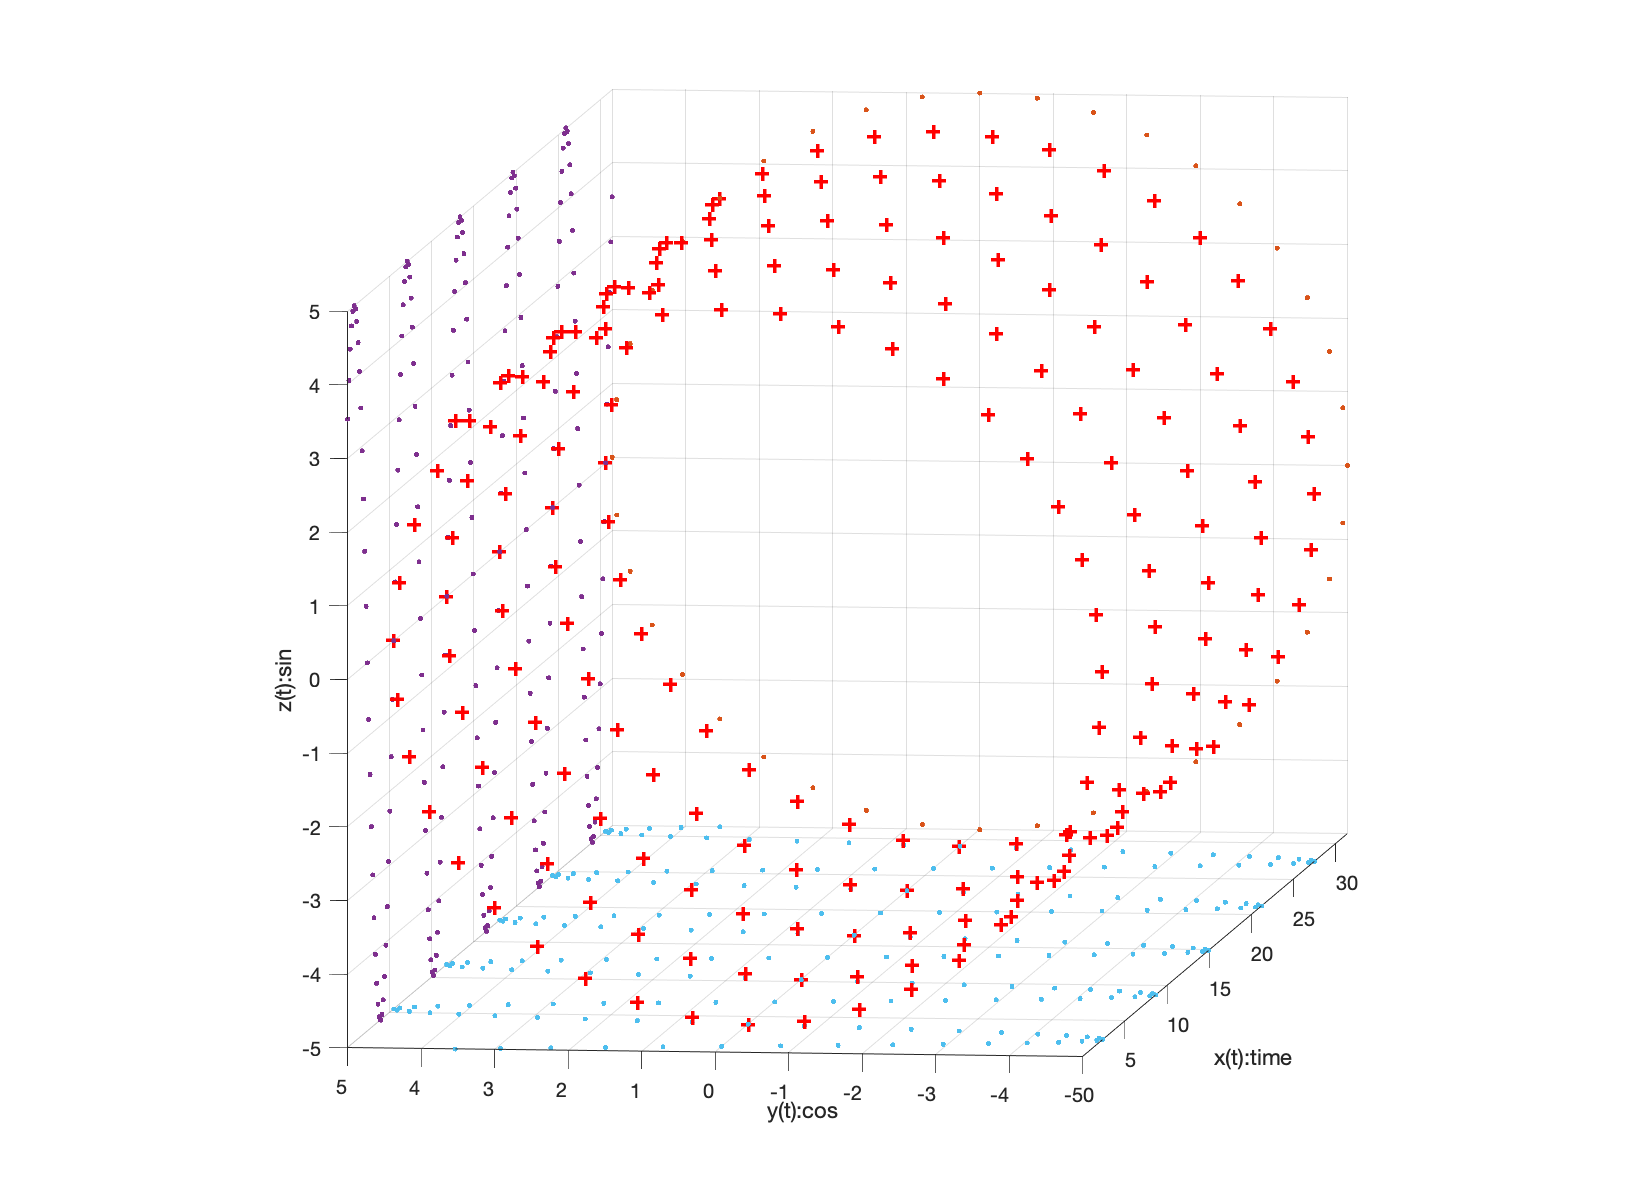
\includegraphics[width=\linewidth]{iqdata2}
	\end{minipage}
	\hfil
	\begin{minipage}{.5\linewidth}
		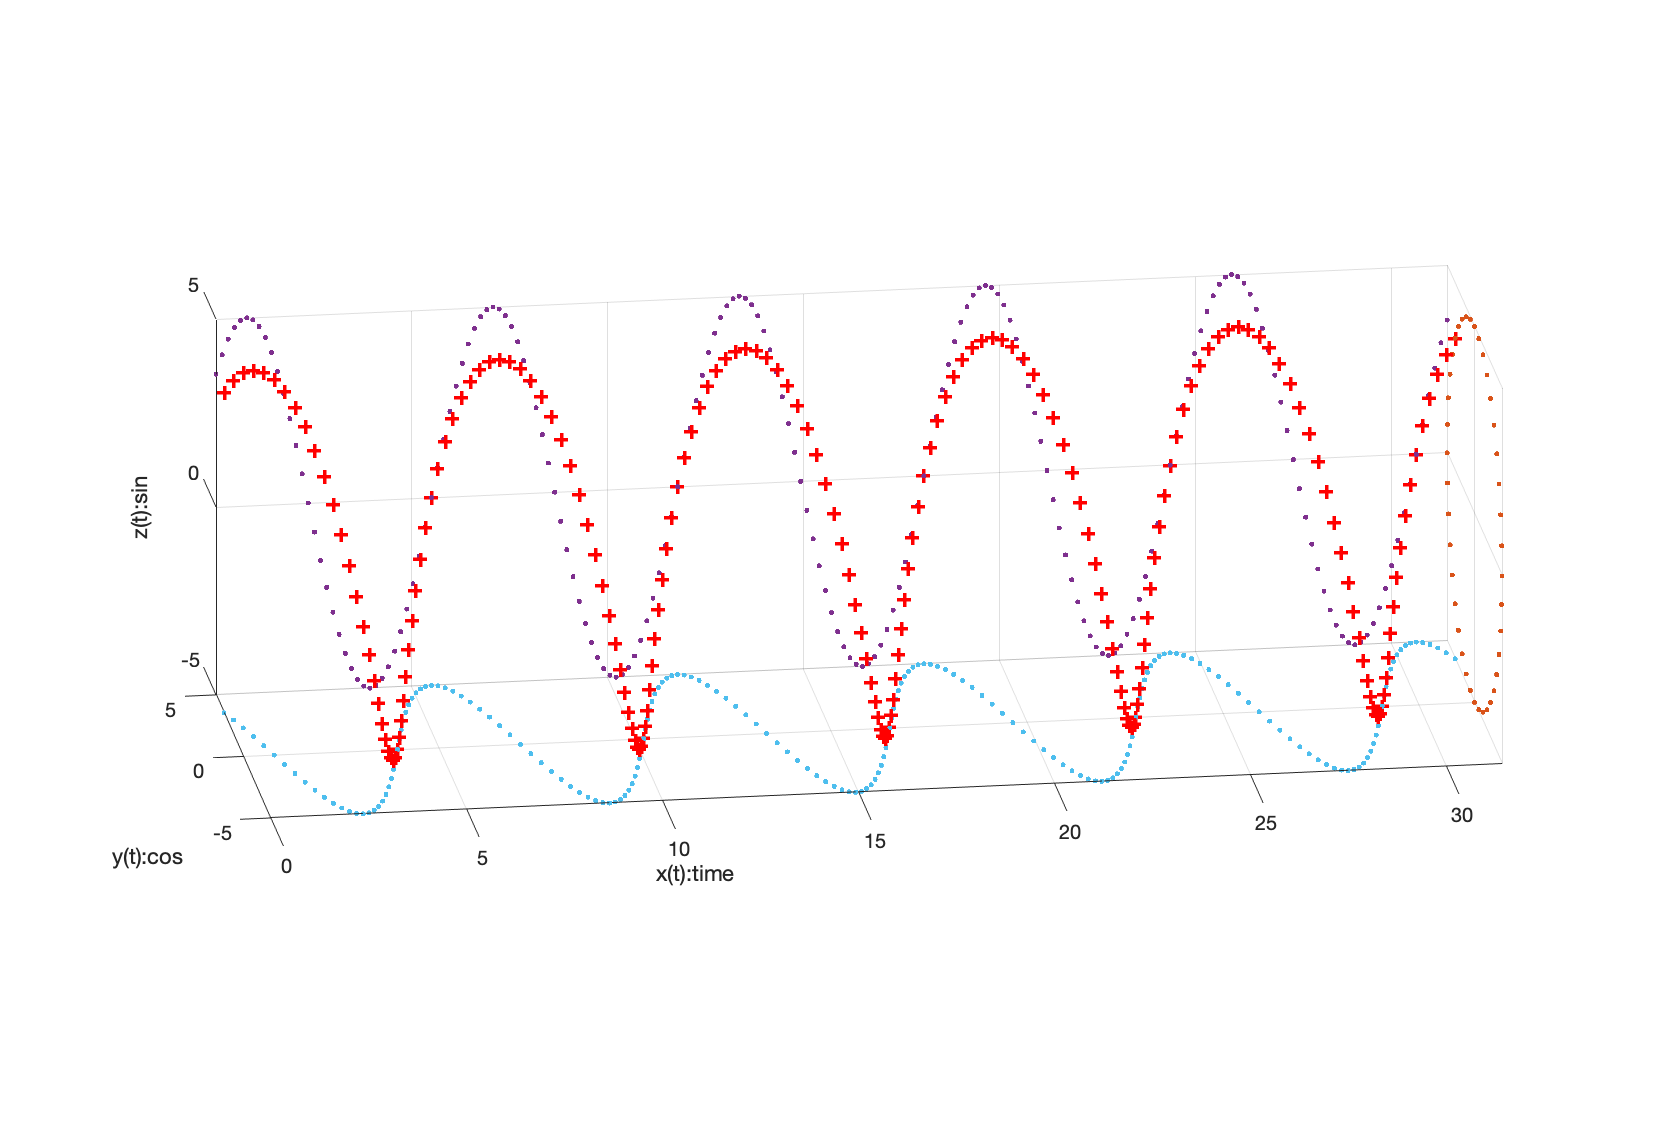
\includegraphics[width=\linewidth]{iqdata3}
		\includegraphics[width=\linewidth]{iqdata4}
	\end{minipage}
	\caption{In-phase and Quadrature Components from Different View Angles}
	\label{fig:iqdata}
\end{figure}

The most common way to represent a wave is to use a series of samples of the momentary amplitude of the signal. However, this method cannot differentiate between a positive or negative frequency since they both generate the same curve, for example,  $\cos(x) = \cos(-x)$. This becomes a problem working with the signal. Mixing (multiplying) two signals and it'll cause multiple solutions due to the uncertainty of the sign. A better way is using I/Q data and representing a wave using in-phase and quadrature components. As shown in Figure~\ref{fig:iqdata}, the signal is plotted in three dimensions. The in-phase component and the quadrature component are the 2D projections of the signal. I/Q data together show the changes in amplitude and phase of a sine wave. The in-phase component indicates the ``real'' signal. For two signals of a positive and a negative frequency, they will have the same in-phase component but reversed quadrature components. Moreover, if the signal is viewed along the time axis, the spiral winds counter-clockwise, which means the frequency is positive. The radius of each circle indicates the peak amplitude of the signal.

Mathematically, for a complex signal $Ae^{i \varphi }$ where $i$ is the imaginary unit, the in-phase component is $I = A\cos(\varphi)$ and the quadrature component is $Q = A\sin(\varphi)$. That is,
\begin{displaymath}
	Ae^{i \varphi } = A \cdot (\cos(\varphi) + i \cdot \sin(\varphi)) = I + Qi
\end{displaymath}
\begin{displaymath}
 A = \sqrt{I^2 + Q^2}  \quad \text{and} \quad \varphi = \tan^{-1}\frac{Q}{I}
\end{displaymath}
%\begin{displaymath}
%\sin(x + \varphi) = \cos(\varphi)\sin(x) + \sin(\varphi)\sin(x+\pi/2)
%\end{displaymath}
%\begin{displaymath}
%\cos(x + \varphi) = \cos(\varphi) \cos(x) + \sin(\varphi)\cos(x+\pi/2)
%\end{displaymath}

In electrical engineering, there are three basic ways to modulate a waveform: Amplitude Modulation (AM), Frequency Modulation (FM) and Phase Modulation (PM). All of them can be achieved by I/Q modulation. Suppose the carrier's frequency is $f$, I/Q modulation is to solve the following equation:
\begin{displaymath}
\texttt{ModulatedSignal} = I \cdot \cos(2 \pi f t) + Q \cdot \sin(2 \pi f t) .
\end{displaymath}
To decode the baseband signal, signal multiplication and low pass filters are needed:
\begin{align*}
I =~&\texttt{lowpass} (\texttt{ModulatedSignal}  \cdot  \cos(2 \pi f t) ) ;\\        
Q=~&\texttt{lowpass} (\texttt{ModulatedSignal}  \cdot \sin(2 \pi f t) ) .
\end{align*}
%\begin{displaymath}
%I = \texttt{lowpass} (\texttt{ModulatedSignal}  \cdot  \cos(2 \pi f t) )
%\end{displaymath}
%\begin{displaymath}
%Q= \texttt{lowpass} (\texttt{ModulatedSignal}  \cdot \sin(2 \pi f t) )
%\end{displaymath}

\subsection{Hand Movements and I/Q Data}
Now we show how hand movements can be regarded as I/Q modulation. As shown in Figure~\ref{fig:soundpath}, the smartphone speaker plays an ultrasound signal $A\cos \left (2\pi f \frac{n}{f_s}\right)$ with the peak amplitude of $A=1$, the frequency $f = 20,000 $~Hz, and the sampling frequency of $f_s = 44,100 $~Hz. At the time $t_p = \frac{n}{f_s}$, the sound propagation path $p$ decreases by $\Delta p$ due to the hand movement. The received signal therefore becomes $2A^\prime_p \cos \left (2\pi f \frac{n}{f_s}  - 2 \pi \frac{\Delta p}{\lambda} - \theta p\right)$, where $2A^\prime_p$ is the new amplitude, the term $2 \pi \frac{\Delta p}{\lambda}$ comes from the phase lag caused by the propagation delay of $\frac{\Delta p}{\lambda}$ and $\lambda$ is the wavelength of the ultrasound. In our system, $\lambda = c/f = \frac{343 \text{~m/s}}{20,000 \text{~Hz}} = 1.72 \text{~cm}$, where $c$ is the speed of sound. The last term $ \theta p$ is the  initial phase, which is caused by the hardware delay and phase inversion due to reflection~\cite{wang2016device}.  
In conclusion, the existence of hand movement changes the amplitude and phase of the original signal. Since I/Q data shows the changes in amplitude and phase of a waveform, we use I/Q data to represent hand movements.

\begin{figure}[h]
	\centering
	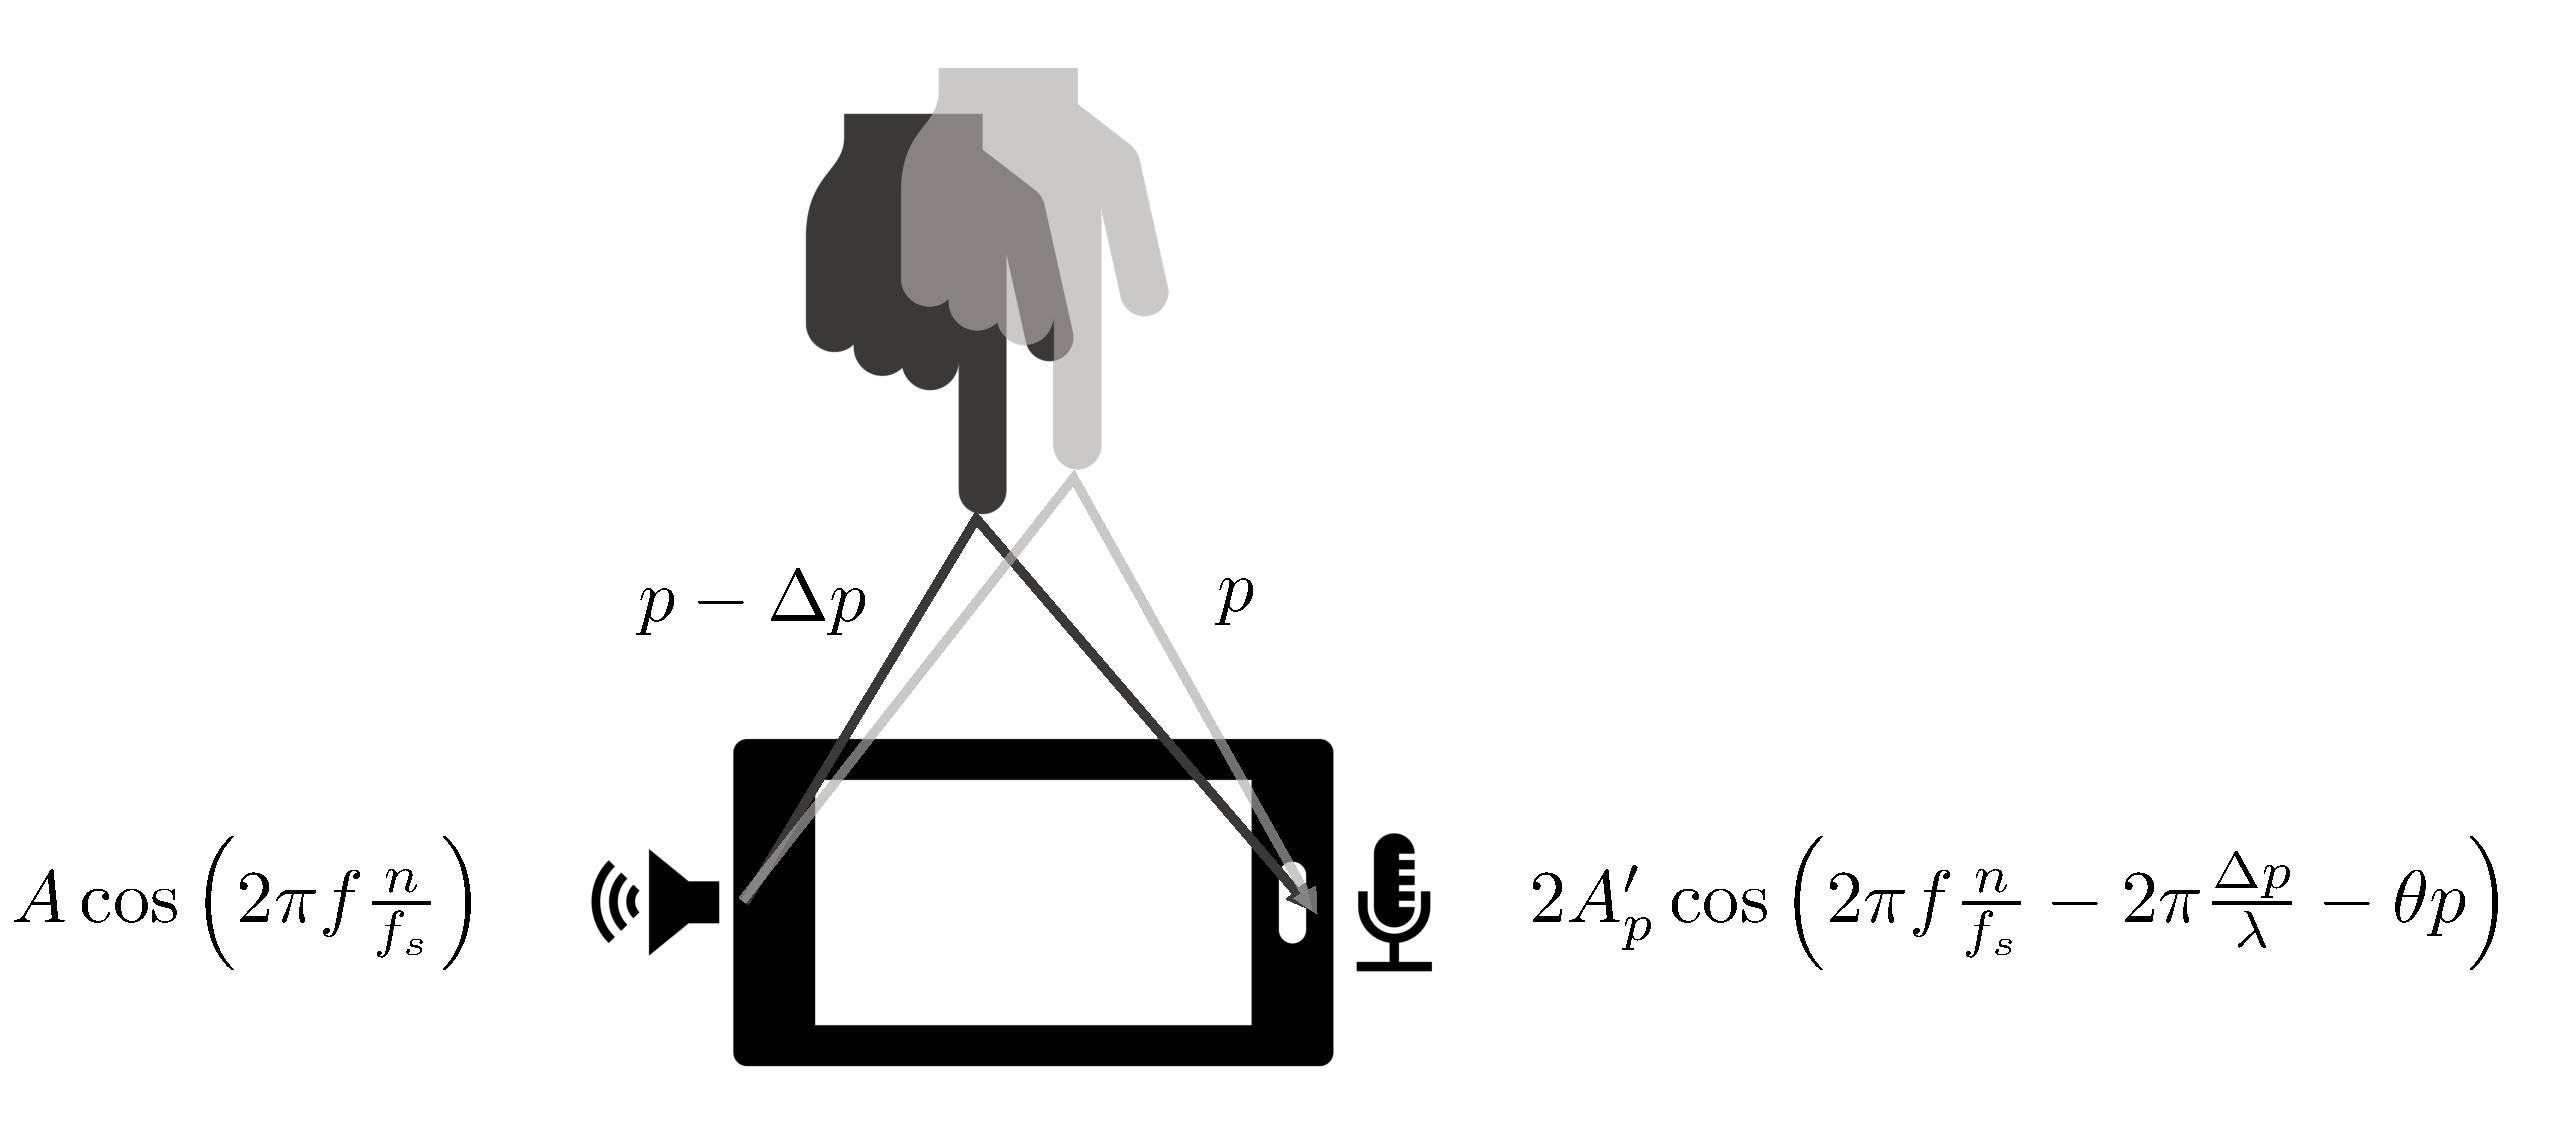
\includegraphics[width=.8\linewidth]{path}
	\caption{Sound Propagation Paths on a Smartphone.}
	\label{fig:soundpath}
\end{figure}

To calculate the in-phase value, we first multiply the received signal by $\cos \left (2\pi f \frac{n}{f_s}\right)$:
\begin{align*}
&2A^\prime_p \cos \left (2\pi f \frac{n}{f_s}  - 2 \pi \frac{\Delta p}{\lambda} - \theta p\right) \times \cos \left (2\pi f \frac{n}{f_s}\right)\\        
=~&A^\prime_p \cos \left (2\pi f \frac{n}{f_s}  - 2 \pi \frac{\Delta p}{\lambda} - \theta p - 2\pi f \frac{n}{f_s}\right)  + A^\prime_p \cos \left (2\pi f \frac{n}{f_s}  - 2 \pi \frac{\Delta p}{\lambda} - \theta p + 2\pi f \frac{n}{f_s}\right)  \\
=~&A^\prime_p \cos \left( - 2 \pi \frac{\Delta p}{\lambda} - \theta p \right)  + A^\prime_p \cos (4\pi f \frac{n}{f_s}  - 2 \pi \frac{\Delta p}{\lambda} - \theta p )  .
\end{align*}

Note that the second term $A^\prime_p \cos \left(4\pi f \frac{n}{f_s}  - 2 \pi \frac{\Delta p}{\lambda} - \theta p \right) $ is a signal of frequency $2f$ and will be removed after applying the low pass filter. Therefore, we get 
\begin{displaymath}
I_p = A^\prime_p \cos \left( - 2 \pi \frac{\Delta p}{\lambda} - \theta p \right) .
\end{displaymath}

Similarly, we can get the quadrature value by multiplying $-\sin \left (2\pi f \frac{n}{f_s}\right)$:
\begin{align*}
&2A^\prime_p \cos \left (2\pi f \frac{n}{f_s}  - 2 \pi \frac{\Delta p}{\lambda} - \theta p\right) \times \left(- \sin \left (2\pi f \frac{n}{f_s}\right)\right)\\        
=~&A^\prime_p \sin \left (2\pi f \frac{n}{f_s}  - 2 \pi \frac{\Delta p}{\lambda} - \theta p - 2\pi f \frac{n}{f_s}\right)  - A^\prime_p \sin \left (2\pi f \frac{n}{f_s}  - 2 \pi \frac{\Delta p}{\lambda} - \theta p + 2\pi f \frac{n}{f_s}\right)  \\
=~&A^\prime_p \sin \left( - 2 \pi \frac{\Delta p}{\lambda} - \theta p \right)  -  A^\prime_p \sin \left(4\pi f \frac{n}{f_s}  - 2 \pi \frac{\Delta p}{\lambda} - \theta p \right)   .
\end{align*}
After low pass filter, we get:
\begin{displaymath}
Q_p = A^\prime_p \sin \left( - 2 \pi \frac{\Delta p}{\lambda} - \theta p \right) .
\end{displaymath}


Combining these two components as the real and imaginary part of a complex signal, we have the complex baseband as follows: 
\begin{displaymath}
\texttt{BasebandSignal} = A^\prime_p e^{-i \left(2 \pi \frac{\Delta p}{\lambda} + \theta p\right)}.
\end{displaymath}

Note that the phase for path $p$ is $\varphi_p = \left(2 \pi \frac{\Delta p}{\lambda} + \theta p\right)$, which changes by $2\pi$ when $\Delta p$ changes by the amount of sound wavelength $\lambda = 1.72 \text{~cm}$. In other words, a small
movement of a few millimeters will significantly change the phase of the received sound wave. 

In conclusion, if there is no hand movement at the time $t_p$, i.e., $\Delta p = 0$,  then $I_p$ and $Q_p$ will be stable. Otherwise, the I/Q components vary like sinusoids.
%:
%\begin{align*}
%I_p = ~&A^\prime_p \cos \left( - \theta p \right) ; \\
%Q_p = ~&A^\prime_p \sin \left( - \theta p \right) .
%\end{align*}

%========================================
%                            Section                             
%======================================== 	 
\section{System Design}
We now provide the system design of {\uu}. The system is built based on Android operating system and tested by Google Nexus 6P smartphones.

In {\uu}, the smartphone speaker would send continuous ultrasound waves with frequency $f = 20,000 $~Hz. The signals are encoded with 16 bit pulse-code modulation (PCM). Then we use the smartphone microphones to catch the reflective signals of the ultrasound simultaneously. Though the smartphone has more than one microphones to support stereo recording, our system only need one channel to calculate the I/Q data.  As shown in Figure~\ref{fig:ultraunlockapp}, we first normalize the signal, then multiply the received signal with $\cos \left (2\pi f \frac{n}{f_s}\right)$ and $-\sin \left (2\pi f \frac{n}{f_s}\right)$. After converting the data to fixed-point data type with 16 word length and 15 fraction length, we feed the data through Cascaded Integrator-Comb (CIC) filters to remove high frequency components and decimate the signal. To achieve better computational efficiency, we do not use a frequency compensate FIR filter after the CIC but directly output the in-phase and quadrature values.



\begin{landscape}
	\begin{figure}[h]
		\centering
		\vspace{-1.7in}
		\includegraphics[width=\linewidth]{UltraUnlockApp}
		\vspace{-1.5in}
		\caption{Android App design for {\uu}}
		\label{fig:ultraunlockapp}
	\end{figure}
\end{landscape}



CIC filter is an optimized class of finite impulse response (FIR) filter combined with an decimator. It provides linear phase response and 
utilizing only delay and addition and subtraction. In other words, it requires no multiplication operations and therefore has less computational costs, which is more suitable to be implemented on smartphones.
%
Our CIC filter is a two section filter (two integrator sand two comb filters)with the decimate ratio of 15 and differential delay of 16. Figure~\ref{fig:CICFilter} shows the frequency response of the CIC filter. We select the parameters so that the first and second zeros of the filter appear at 183 Hz and 366 Hz. The pass-band of the CIC filter is 0 - 100 Hz, which corresponds to the movements with a speed lower than 0.86 m/s when the wavelength is 1.72 cm. 

\begin{figure}[h]
	\centering
	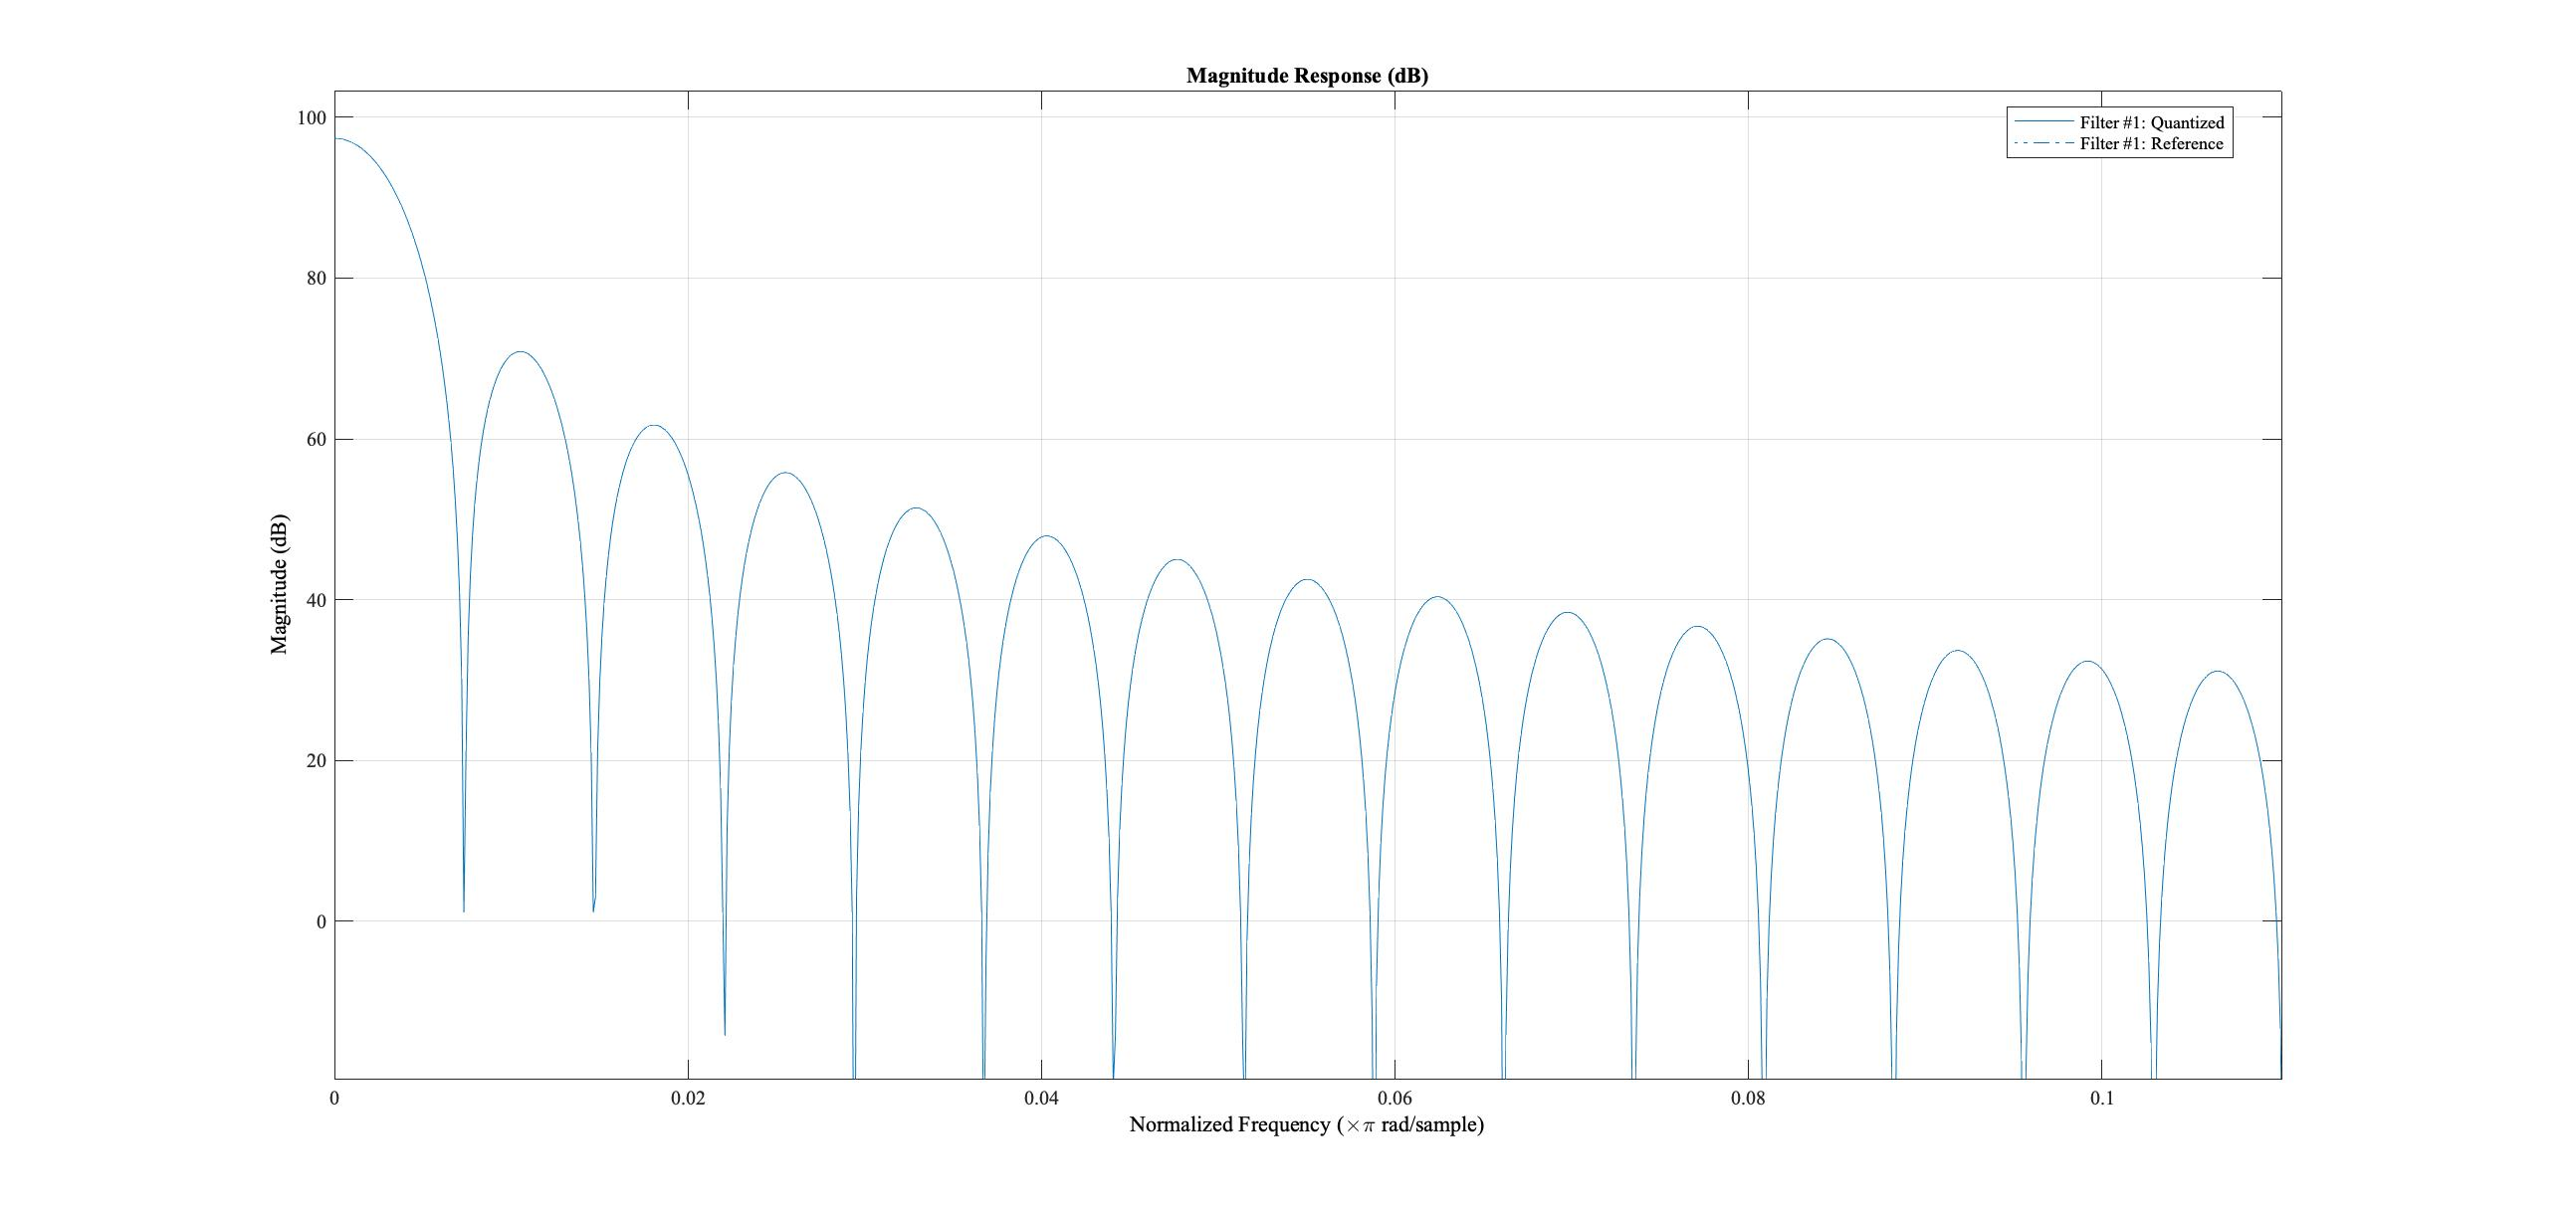
\includegraphics[width=.9\linewidth]{CICFilter}
	\caption{Frequency Response of the Cascaded Integrator-Comb Filter}
	\label{fig:CICFilter}
\end{figure}

As discussed in Section~\ref{sec:handIQ}, the in-phase and quadrature components are a good indicator of the path changes. In detail, the I/Q waveforms remain static when the hand is not moving and vary like sinusoids when the hand moves. Different hand movements generate different sinusoids, which can be trained by a Long Short-Term Memory LSTM network for classification.  We use the same LSTM network as discussed in Section~\ref{sec:LSTM}, but with different parameter settings.

%========================================
%                            Section                             
%======================================== 	 
\section{Experiment Results}

We implemented the {\uu} on a Google Nexus 6P smartphone and first validate the correlation between hand movements and I/Q data.
Three screenshots are shown in Figure~\ref{fig:realIQ}. The yellow lines are the quadrature components and the blue lines are the in-phase components. The x-axis is the indexes of samples. In each figure, 256 samples are shown, which spans in the time period of $256/294\times4410/44100 = 0.087$ s. (256 is the buffer size of the array plot, 294 is the sampling rate after CIC filter, 4410 is the frame size of audio recorder, and 44100 is the sampling frequency of the carrier signal.) As shown in Figure~\ref{fig:realIQ}, when there is no hand movement, the I/Q data are stable. When user put one hand parallel to the phone and move towards the screen, then I/Q value become regular sinusoids. If the user conduct an open-close gesture (make a loose fist and then spread all fingers wide), the I/Q data are still sinusoidal but they become less regular. Note that these screen shots cannot represent the whole changes caused by hand movement, since a whole gesture usually costs about 0.3-1 second, which spans 3 to 12 frames.


\begin{figure}[h]
	\centering
	\begin{minipage}{.6\linewidth}
		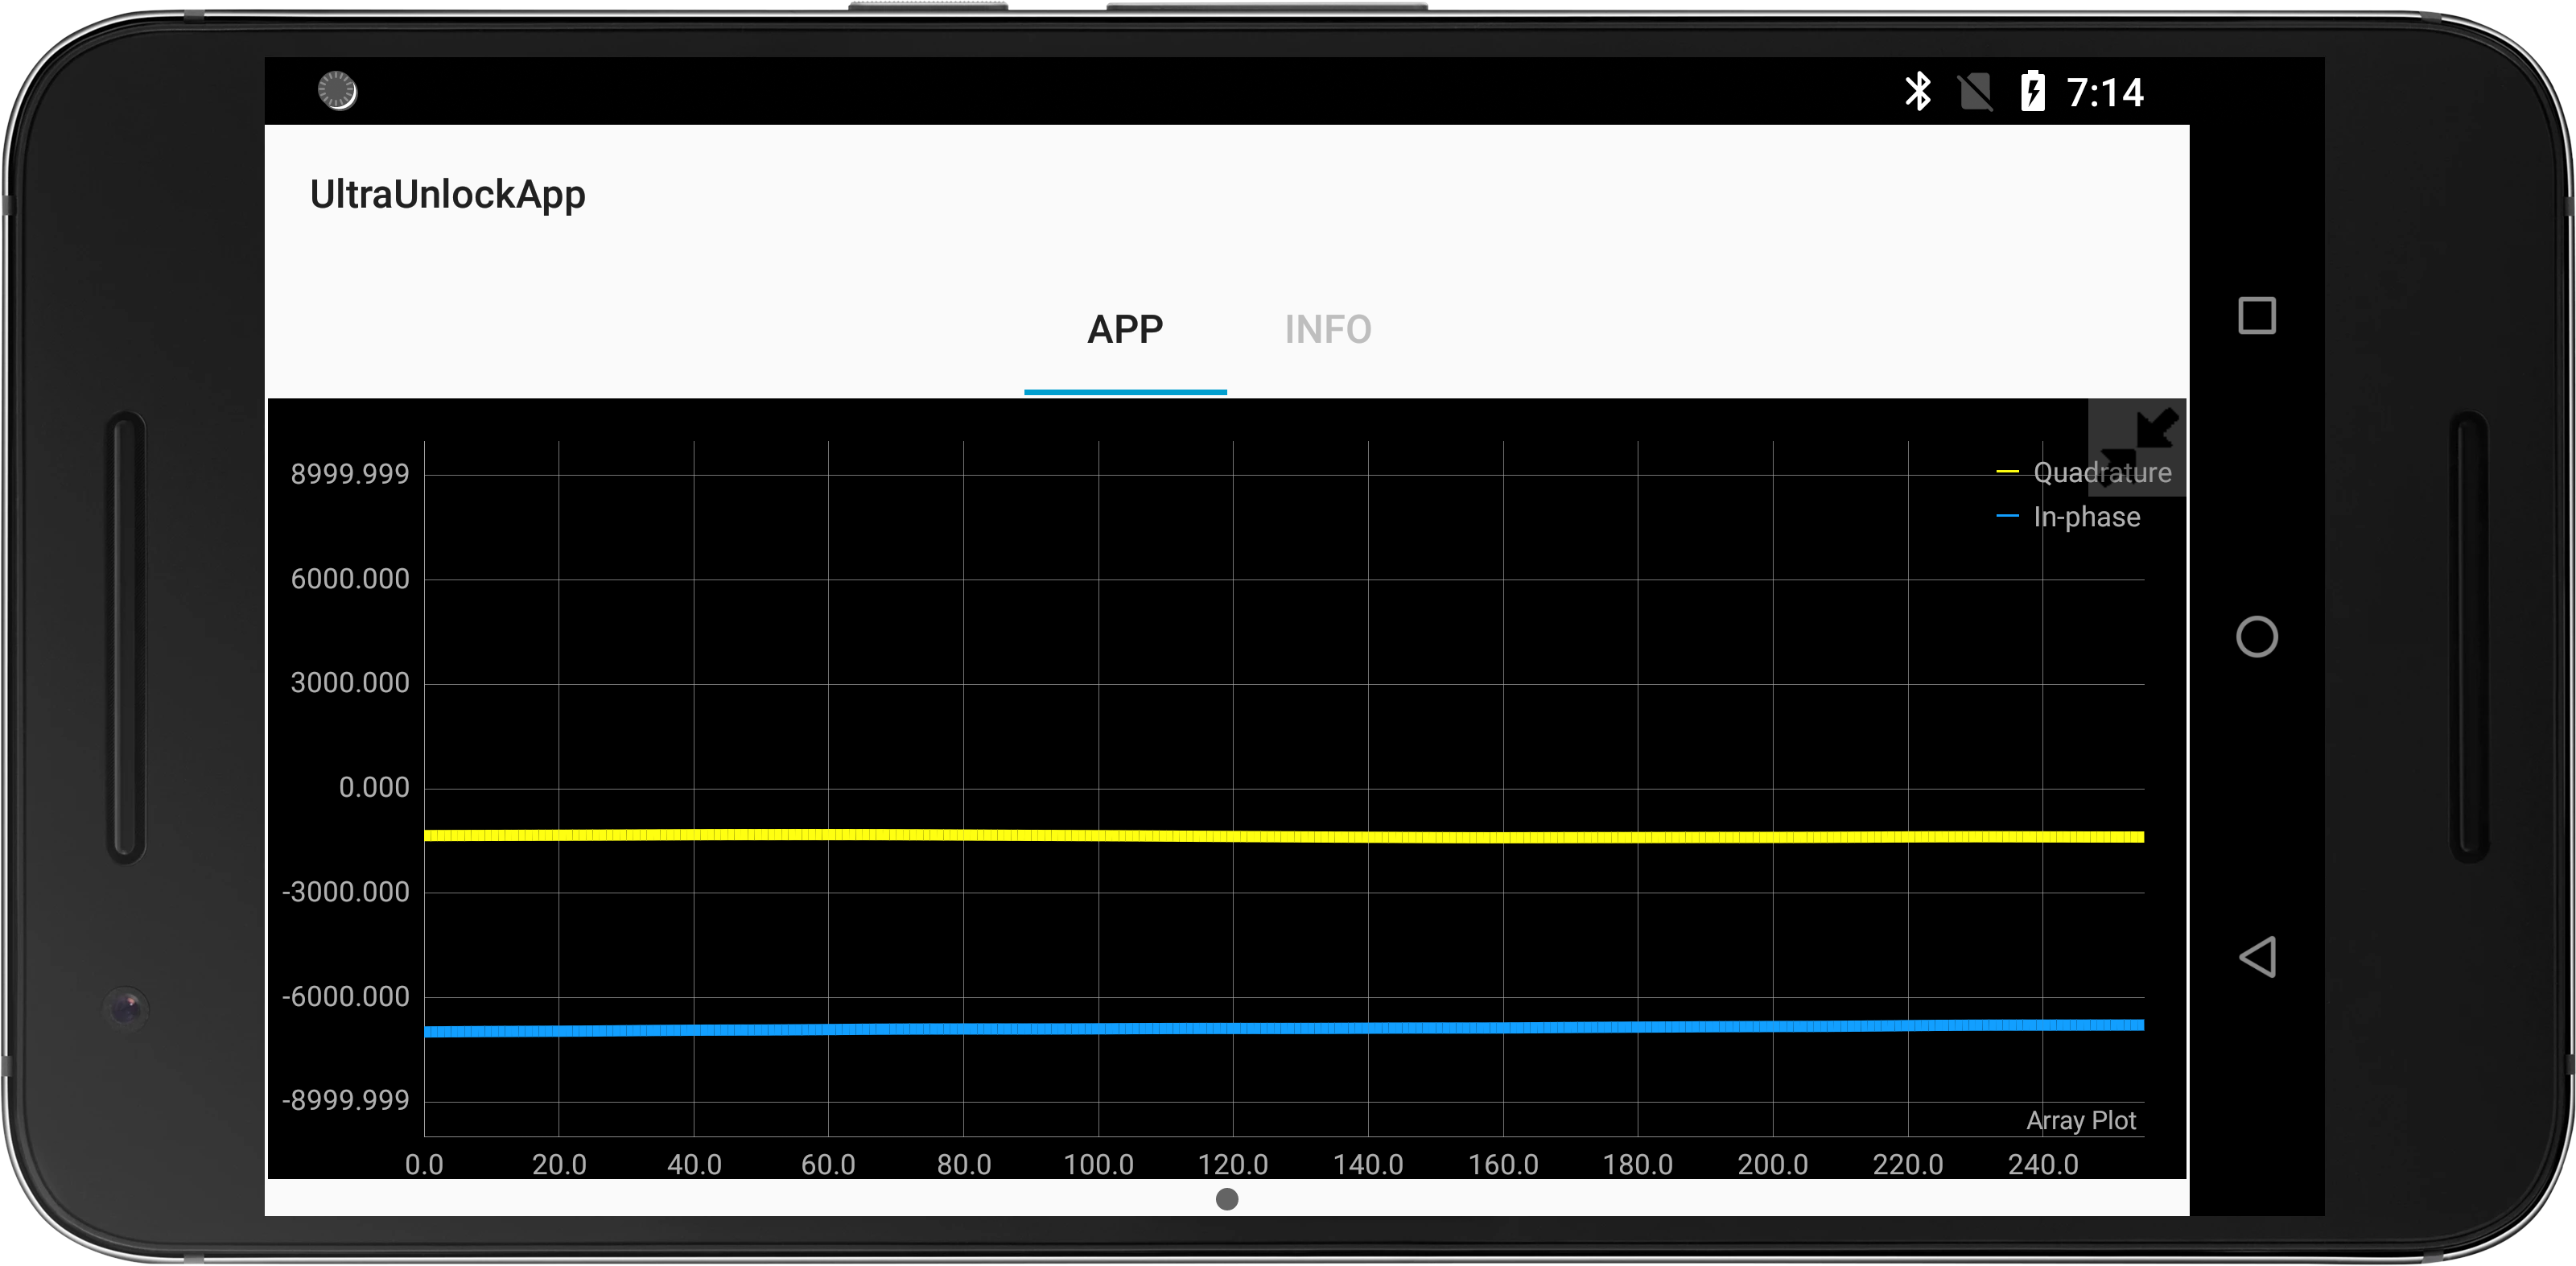
\includegraphics[width=\linewidth]{realiqdata0}
		\subcaption{No Hand Movement}
		\vspace{.1in}
		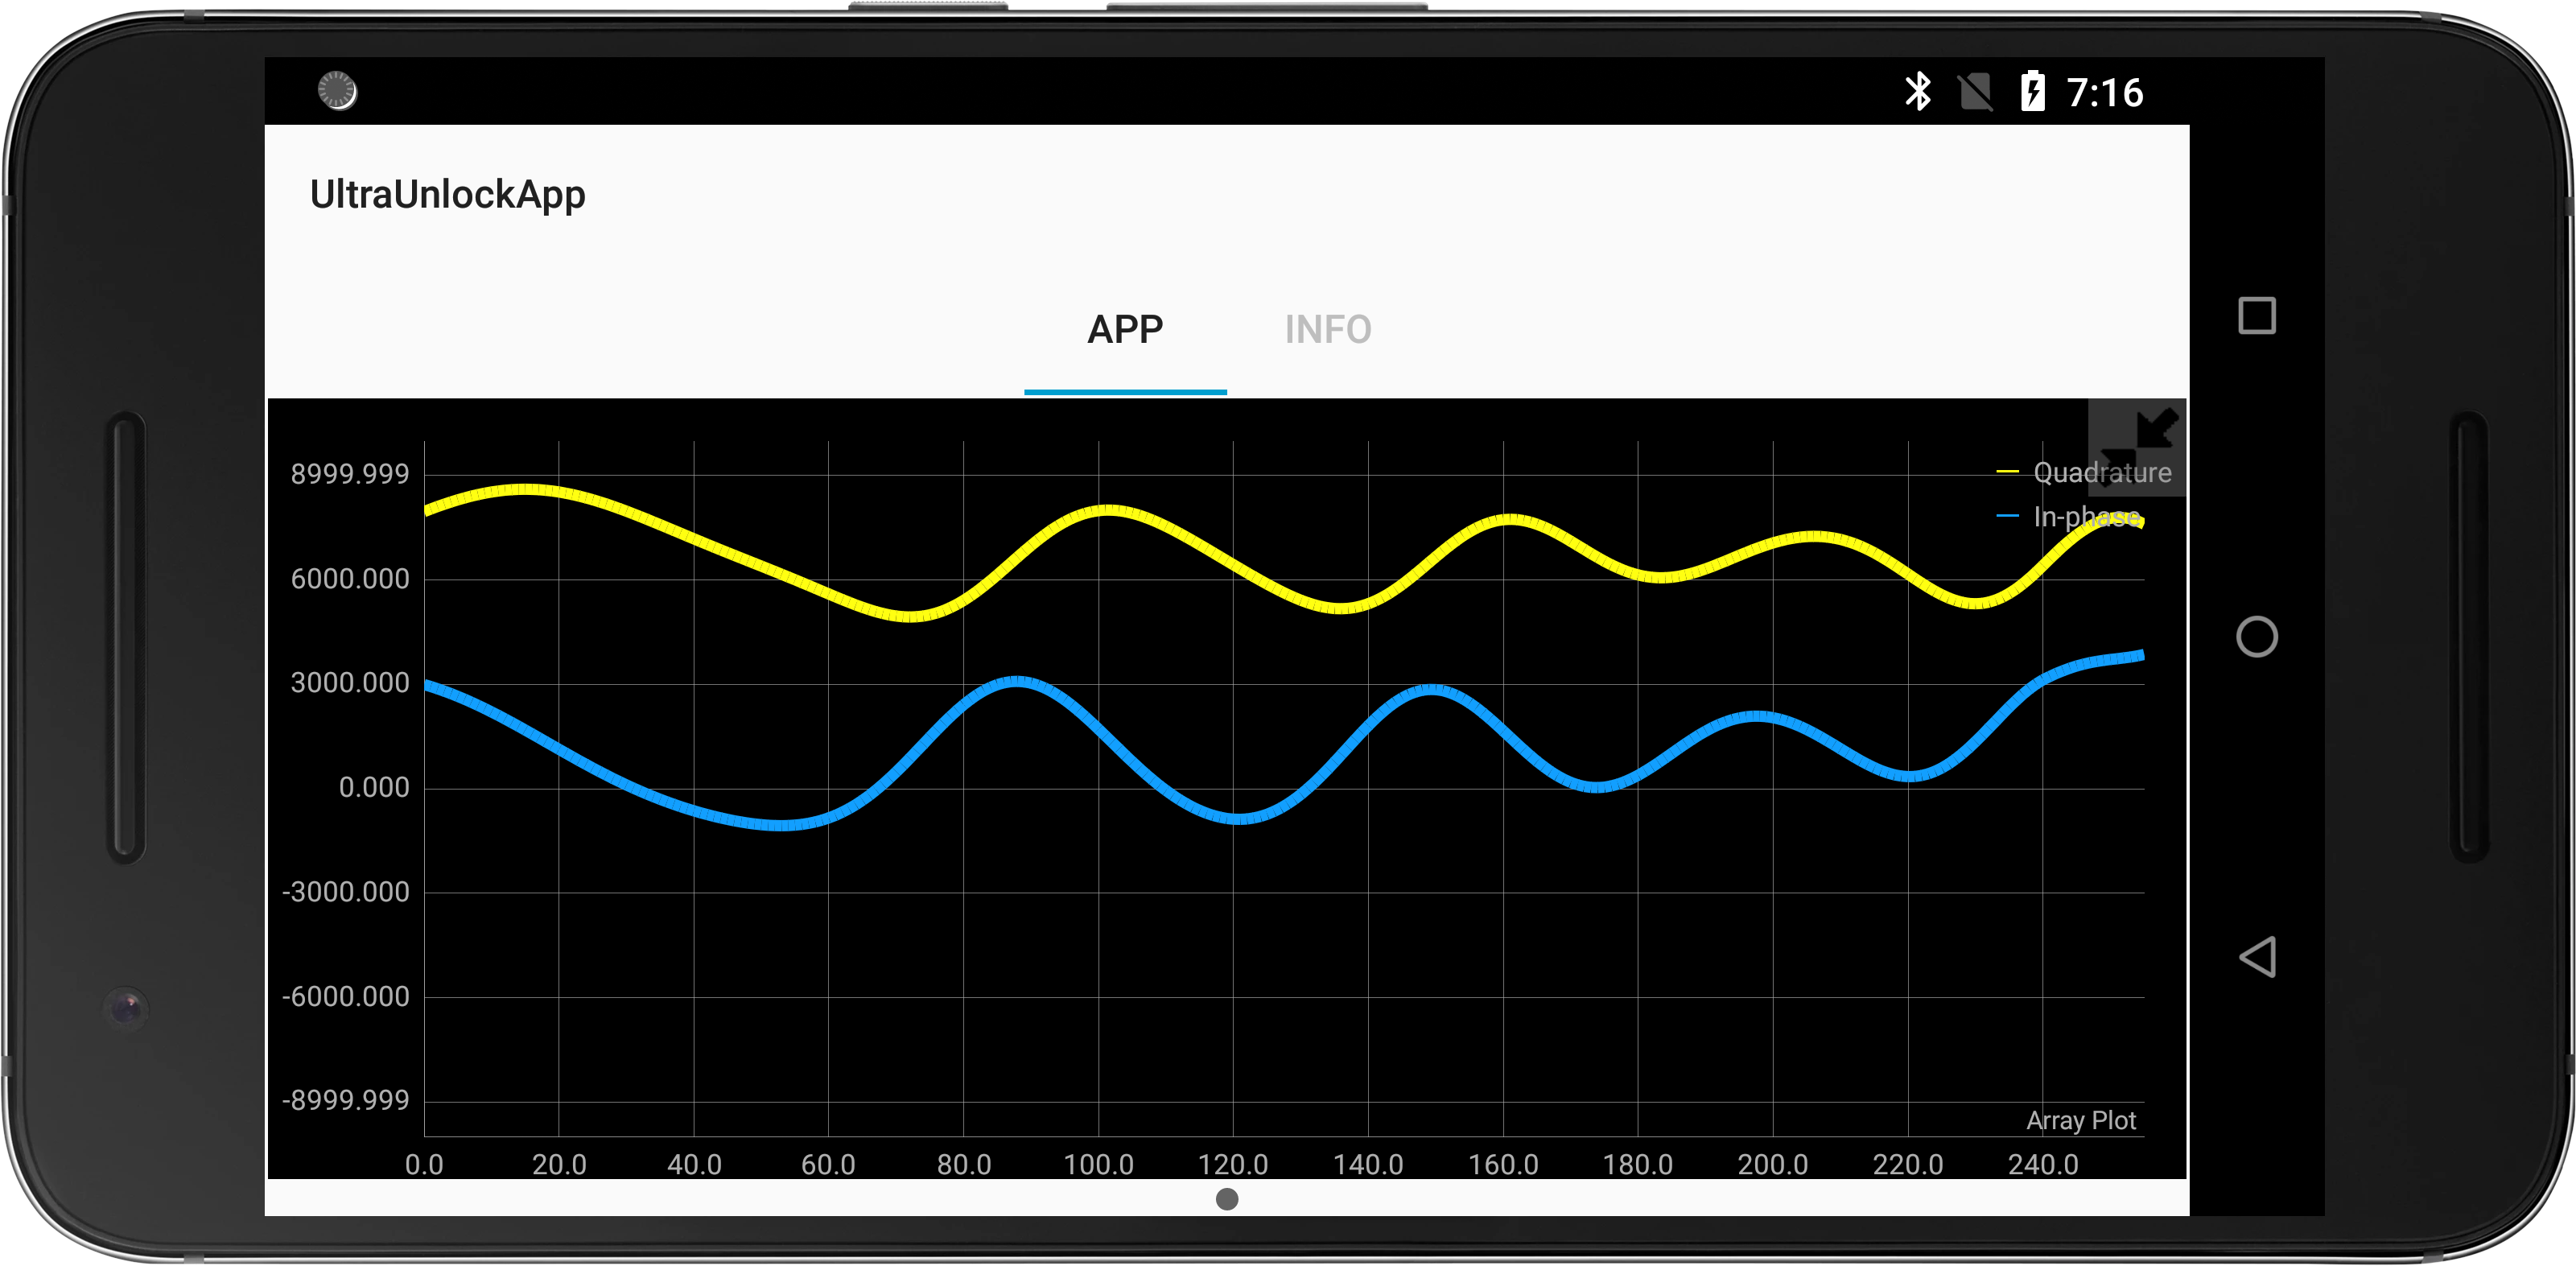
\includegraphics[width=\linewidth]{realiqdata1}
		\subcaption{One Hand Moving Towards the Phone}
		\vspace{.1in}
		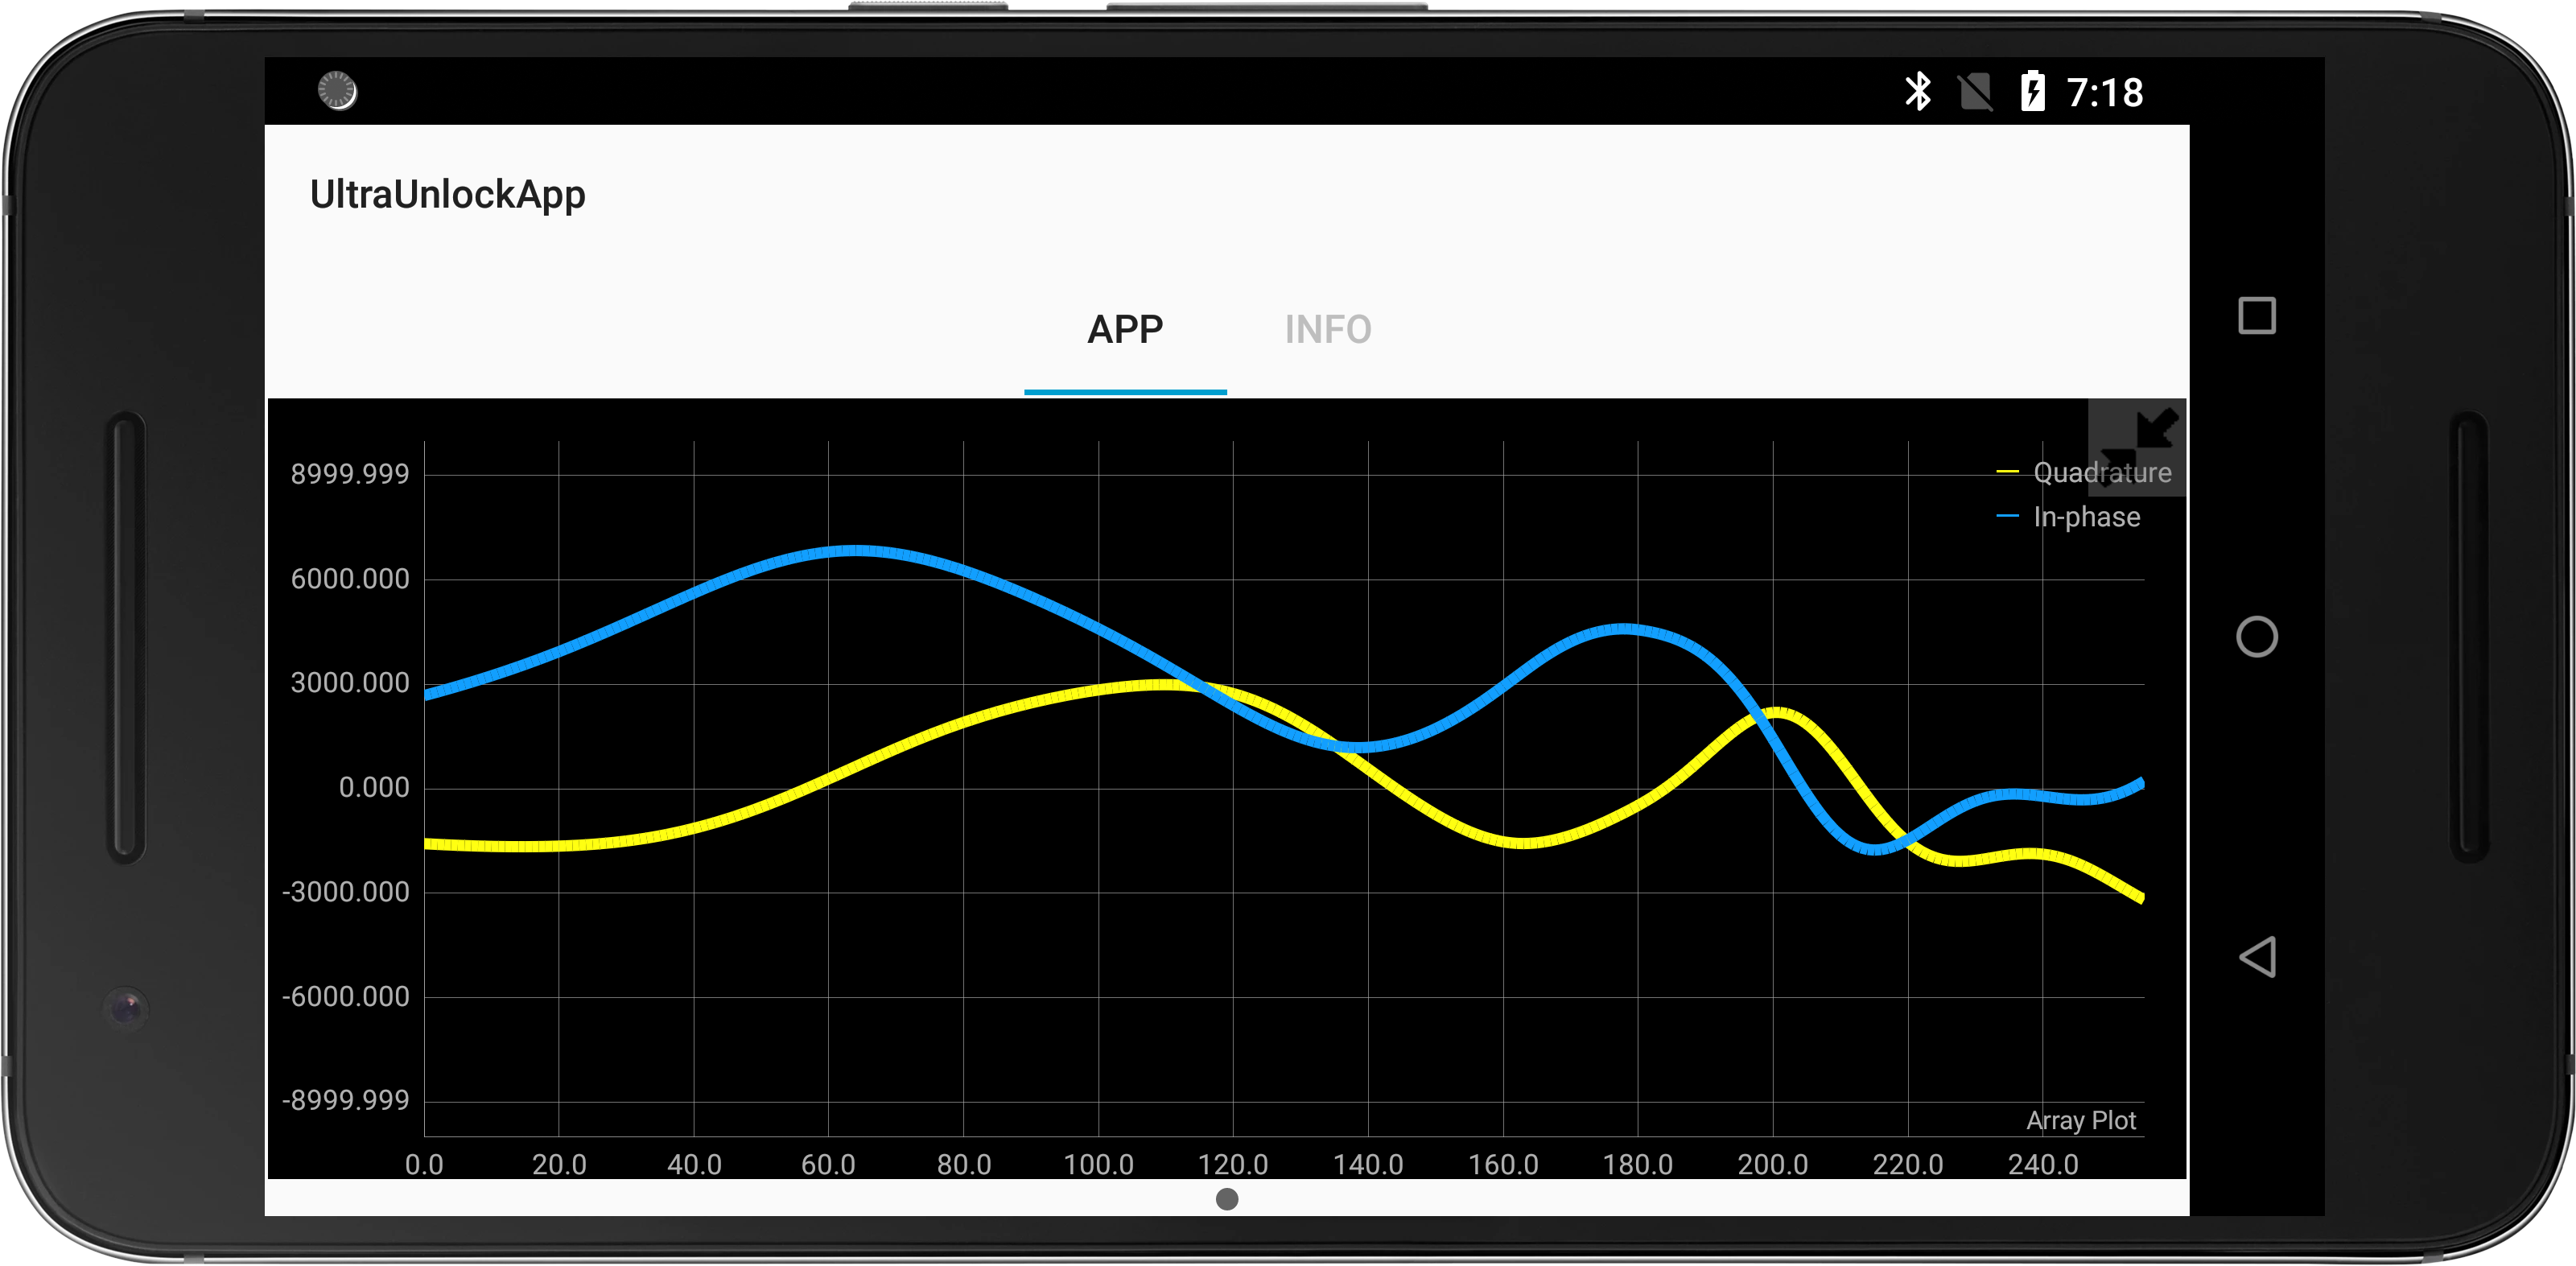
\includegraphics[width=\linewidth]{realiqdata2}
		\subcaption{Open-Close Gesture}
	\end{minipage}
	\caption{Screenshots of the UltraUnlockApp}	
	\label{fig:realIQ}
\end{figure}

\begin{figure}[!h]
	\centering
	\includegraphics[width=.8\linewidth]{androidiqdata1}
	\begin{minipage}{.4\linewidth}
		\includegraphics[width=\linewidth]{androidiqdata2}
	\end{minipage}
	\hfil
	\begin{minipage}{.5\linewidth}
		\includegraphics[width=\linewidth]{androidiqdata3}
		\includegraphics[width=\linewidth]{androidiqdata4}
	\end{minipage}
	\caption[I/Q Components Collected by UltraUnlockApp]{I/Q Components from Different View Angles. The hand first move dowards towards the smartphone, then move upwards.}
	\label{fig:androidiqdata}
\end{figure}

Figure~\ref{fig:androidiqdata} shows the I/Q data collected when the user moves the hand down and up. The phase of of the I/Q data inverses at 0.24 second, which indicates the direction change of the hand movement. Moreover, we noticed that there are 4 gull peaks and valleys before the hand change the direction. Combining with the fact that the wavelength of the signal is 1.72 cm, we know that the path changes $1.72 \times 4 = 6.88$ cm. In other words, in 0.2 second, the user moves one hand towards the smartphone by 3.44 cm. Note that this distance is calculated based on the assumption that the user hand moves in one dimension. However, in reality, user hands moves in 3D. Fortunately, smartphones nowadays are usually equipped with more than two speakers and more than two microphones, which enable {\uu} to locate user hands in 3D. Due to time limit, the current {\uu}App does not have this feature yet. In future work, we will implement this feature, as more dimensions of features will also increase the accuracy of user authentication.

\begin{figure}[h]
	\centering
	\begin{minipage}{.6\linewidth}
		\includegraphics[width=\linewidth]{gestures}
	\end{minipage}
	\caption{Gestures tested in {\uu}.}	
	\label{fig:gestures}
\end{figure}


Our current machine learning modal only have two dimensions of features: the amplitude and the phase calculated from I/Q data. We tested our {\uu} system on 6 people and 3 gestures. Each user is asked to perform the same gestures for 20 times where we use half of them to train the LSTM network and the other half to test the model. The three gestures are: up-down, open-close, and drawing ``8'' in the air as shown in Figure~\ref{fig:gestures}. The 6 people are 3 females and 3 males aging 20-30. 


\begin{figure}[!h]
	\centering
	\begin{minipage}{.35\linewidth}
		\includegraphics[width=\linewidth]{gestureCFM}
		\vspace{.05in}
	\end{minipage}
	
	\centering
	%	\resizebox{\linewidth}{!}{
	\begin{tabular}{lr}
		\toprule
		Accuracy: 90.89\% & \hspace{-.55in} Error Rate: 9.11\% \\
		Precision: 92.04\% & \hspace{-.55in} True Positive Rate (Sensitivity/Recall): 91.00\% \\
		$F_1$ Score: 0.915 & \hspace{-.55in} True Negative Rate (Specificity): 95.10\% \\
		False Negative Rate: 9.00\%  & \hspace{-.55in} False Positive Rate: 4.90\% \\
		\bottomrule
	\end{tabular}
	\caption{The Confusion Matrix of the Gesture Classification Result.
	}
	\label{fig:gestureCFM}
\end{figure}

\begin{figure}[!h]
	\centering
	\begin{minipage}{.45\linewidth}
		\includegraphics[width=\linewidth]{userCFM}
		\vspace{.05in}
	\end{minipage}
	
	\centering
	%	\resizebox{\linewidth}{!}{
	\begin{tabular}{lr}
		\toprule
		Accuracy: 78.47\% & \hspace{-.55in} Error Rate: 21.53\% \\
		Precision: 77.74\% & \hspace{-.55in} True Positive Rate (Sensitivity/Recall): 77.69\% \\
		$F_1$ Score: 0.775 & \hspace{-.55in} True Negative Rate (Specificity): 95.68\% \\
		False Negative Rate: 22.31\%  & \hspace{-.55in} False Positive Rate: 4.32\% \\
		\bottomrule
	\end{tabular}
	\caption{The Confusion Matrix of the User Classification Result.
	}
	\label{fig:userCFM}
\end{figure}

The classification results of 3 gestures are shown in Figure~\ref{fig:gestureCFM}. The average accuracy is 90.89\% and the up-down gesture has the least false negative rate. The classification results of user identification is shown in Figure~\ref{fig:userCFM}, where the average accuracy is 78.47\%.  Note that the true negative rate (specificity) is 95.68\% and the false positive rate is 4.32\%, which means there is a higher chance that a legitimate user would be rejected than the chance that an attacker get accepted by the phone. Though such setting will provide more security to the smartphone, the overall accuracy is not satisfactory. There are at least three ways to further increase it, and we leave it for future work:
\begin{itemize}
	\item Utilizing more speakers and microphones. In this chapter, we only utilizing one microphone and one speaker on the smartphone. However, most smartphones nowadays support stereo audio, which means the device is equipped with at least a pair of microphones and a pair of speakers. If all sensors and transmitters are adopted, we will increase the signal channel from $1\times1$ to $2 \times2$. If doing so, {\uu} will be able to localize the hand in three dimensions and the feature vectors will increase from 2 to 8. Intuitively, the performance of the classification model will be improved with more features. However, there would also be many challenges to achieve the upgrades. For example, we need to propose effective and efficient algorithms to deal with the interference caused by the simultaneous signals.
	\item Using chirp signals instead of a single-frequency signal.
	\item Extracting more information from I/Q data instead of directly feeding them to LSTM networks.
	\item Recruiting more volunteers and testing more gestures.
	\item Evaluating the performance of {\uu} under different settings. 
\end{itemize}







%========================================
%                            Section                             
%======================================== 	 
\section{Conclusion}
In this chapter, we demonstrated how to use I/Q data to represent hand movements and show the potential of using the I/Q data for smartphone authentication. 
%========================================
%                            Chapter                            
%======================================== 
\chapter{{\mv}: A Spoof-proof Voice Authentication System for Smartphones}

	Voice authentication is drawing increasing attention and becomes an attractive alternative to passwords for mobile authentication. However, existing voice authentication systems are vulnerable to various spoofing attacks. For example, attackers can record the victim's voice in person or online, then replay the recording and access the victim's devices illegally. 
We propose \shortname, a spoof-proof voice authentication system which not only differentiate different people but also differentiate live people and electronic devices. The idea is to utilize the self demodulation effect and acoustic attenuation effect when sound signals transmit through human bodies. Our system can defend the smartphone's voice authentication system against 3 attack scenarios, each contains 3 attack types. Experiments show  {\shortname} can identify different users with 94.33\% accuracy and defend voice spoofing attacks with at least 93.67\% accuracy. 
%========================================
%                            Section                             
%======================================== 	 


%\IEEEraisesectionheading{\section{Introduction}\label{sec:introduction}}
\section{Introduction}
% Computer Society journal (but not conference!) papers do something unusual
% with the very first section heading (almost always called "Introduction").
% They place it ABOVE the main text! IEEEtran.cls does not automatically do
% this for you, but you can achieve this effect with the provided
% \IEEEraisesectionheading{} command. Note the need to keep any \label that
% is to refer to the section immediately after \section in the above as
% \IEEEraisesectionheading puts \section within a raised box.




% The very first letter is a 2 line initial drop letter followed
% by the rest of the first word in caps (small caps for compsoc).
% 
% form to use if the first word consists of a single letter:
% \IEEEPARstart{A}{demo} file is ....
% 
% form to use if you need the single drop letter followed by
% normal text (unknown if ever used by the IEEE):
% \IEEEPARstart{A}{}demo file is ....
% 
% Some journals put the first two words in caps:
% \IEEEPARstart{T}{his demo} file is ....
% 
% Here we have the typical use of a "T" for an initial drop letter
% and "HIS" in caps to complete the first word.
%\IEEEPARstart{T}{his} demo file is intended to serve as a ``starter file''
%for IEEE Computer Society journal papers produced under \LaTeX\ using
%IEEEtran.cls version 1.8b and later.
%% You must have at least 2 lines in the paragraph with the drop letter
%% (should never be an issue)
%I wish you the best of success.
%
%\hfill mds
%
%\hfill August 26, 2015

%\subsection{Subsection Heading Here}
%Subsection text here.

% needed in second column of first page if using \IEEEpubid
%\IEEEpubidadjcol

%\subsubsection{Subsubsection Heading Here}
%Subsubsection text here.


% An example of a floating figure using the graphicx package.
% Note that \label must occur AFTER (or within) \caption.
% For figures, \caption should occur after the \includegraphics.
% Note that IEEEtran v1.7 and later has special internal code that
% is designed to preserve the operation of \label within \caption
% even when the captionsoff option is in effect. However, because
% of issues like this, it may be the safest practice to put all your
% \label just after \caption rather than within \caption{}.
%
% Reminder: the "draftcls" or "draftclsnofoot", not "draft", class
% option should be used if it is desired that the figures are to be
% displayed while in draft mode.
%
%\begin{figure}[!t]
%\centering
%\includegraphics[width=2.5in]{myfigure}
% where an .eps filename suffix will be assumed under latex, 
% and a .pdf suffix will be assumed for pdflatex; or what has been declared
% via \DeclareGraphicsExtensions.
%\caption{Simulation results for the network.}
%\label{fig_sim}
%\end{figure}

% Note that the IEEE typically puts floats only at the top, even when this
% results in a large percentage of a column being occupied by floats.
% However, the Computer Society has been known to put floats at the bottom.


% An example of a double column floating figure using two subfigures.
% (The subfig.sty package must be loaded for this to work.)
% The subfigure \label commands are set within each subfloat command,
% and the \label for the overall figure must come after \caption.
% \hfil is used as a separator to get equal spacing.
% Watch out that the combined width of all the subfigures on a 
% line do not exceed the text width or a line break will occur.
%
%\begin{figure*}[!t]
%\centering
%\subfloat[Case I]{\includegraphics[width=2.5in]{box}%
%\label{fig_first_case}}
%\hfil
%\subfloat[Case II]{\includegraphics[width=2.5in]{box}%
%\label{fig_second_case}}
%\caption{Simulation results for the network.}
%\label{fig_sim}
%\end{figure*}
%
% Note that often IEEE papers with subfigures do not employ subfigure
% captions (using the optional argument to \subfloat[]), but instead will
% reference/describe all of them (a), (b), etc., within the main caption.
% Be aware that for subfig.sty to generate the (a), (b), etc., subfigure
% labels, the optional argument to \subfloat must be present. If a
% subcaption is not desired, just leave its contents blank,
% e.g., \subfloat[].


% An example of a floating table. Note that, for IEEE style tables, the
% \caption command should come BEFORE the table and, given that table
% captions serve much like titles, are usually capitalized except for words
% such as a, an, and, as, at, but, by, for, in, nor, of, on, or, the, to
% and up, which are usually not capitalized unless they are the first or
% last word of the caption. Table text will default to \footnotesize as
% the IEEE normally uses this smaller font for tables.
% The \label must come after \caption as always.
%
%\begin{table}[!t]
%% increase table row spacing, adjust to taste
%\renewcommand{\arraystretch}{1.3}
% if using array.sty, it might be a good idea to tweak the value of
% \extrarowheight as needed to properly center the text within the cells
%\caption{An Example of a Table}
%\label{table_example}
%\centering
%% Some packages, such as MDW tools, offer better commands for making tables
%% than the plain LaTeX2e tabular which is used here.
%\begin{tabular}{|c||c|}
%\hline
%One & Two\\
%\hline
%Three & Four\\
%\hline
%\end{tabular}
%\end{table}


% Note that the IEEE does not put floats in the very first column
% - or typically anywhere on the first page for that matter. Also,
% in-text middle ("here") positioning is typically not used, but it
% is allowed and encouraged for Computer Society conferences (but
% not Computer Society journals). Most IEEE journals/conferences use
% top floats exclusively. 
% Note that, LaTeX2e, unlike IEEE journals/conferences, places
% footnotes above bottom floats. This can be corrected via the
% \fnbelowfloat command of the stfloats package.


\subsection{The Popularity of Voice Authentication on Smartphones}

According to reports issued by several market-research firms, the total number of smartphone users worldwide is over 3 billion this year and is expected to reach 3.9 billion by 2023~\cite{report2018newzoo,report2019forrester}. The rapid increasing use of smartphones is actuating the need for better protection. User authentication on smartphones has thus been an important area of research. 

Survey papers~\cite{vongsingthong2014survey,mahfouz2017survey,shankar2018survey} have compared the strengths and limitations of existing authentication methods, from knowledge-based methods such as PIN or password, to identity-based methods such as fingerprint and face.
%
PIN or password are the most widely used authentication methods. However, when the users have wet or dirty fingers, or wear gloves on their hands, such touchscreen-related authentication methods will not work. The fingerprint authentication suffers from the same problem. As for face recognition, it stops working when users are wearing moisturizing mask sheets or other head wearables such as ski goggles. In the aforementioned scenarios, voice authentication provides better convenience to users and thus a great alternative.


In fact, voice authentication has been adopted in a wide variety of smartphone applications. 
For example, Android users can say ``Ok Google'' to access Google assistant directly~\cite{onlinegoogle}; the Tencent company adopts Voiceprint to provide securely, faster and easier log-ins to WeChat accounts, available on both Android and iOS platforms~\cite{onlinewechat}; the BioTrust uses voice biometrics to allow elderly and sick people to order prescription medication without the need to leave the house~\cite{onlinebio}; the Citi bank uses voice biometrics authentication system for phone banking, which reduces the number of tedious security questions~\cite{onlineciti}; the LMH Blockchain adopts Say-Tec~\cite{onlinesaytec} to authenticate, validate, process, and protect users' blockchain assets and cryptocurrency by voice~\cite{onlineblockchain}.
%
Based on a market research report published in 2019~\cite{onlinemarket}, the speech and voice recognition market is expected to grow from 
 \$7.5 billion as in 2018 to  \$21.5 billion by 2024. 
 
 

\subsection{Voice Spoofing Attacks}\label{sec:spoof}
Despite of the increasing trend for the adopting of voice authentication, this method is not unassailable, just like other methods. Researchers have found that voice authentication system are vulnerable to the following four attacks~\cite{wu2015spoofing}: impersonation attack, replay attack, speech synthesis, and voice conversion.
\begin{itemize}
	\item  Impersonation attack refers to the scenario where an attacker tries to mimic the legitimate user’s voice without any computer-aided technology.
	\item Replay attack refers to the scenario where an attacker replays a pre-recorded speech sample collected from the legitimate user. 
	\item Speech synthesis refers to the scenario where an attacker generates intelligible, natural-sounding artificial speech from text.
	\item Voice conversion refers to the scenario where an attacker converts his speech signals to an artificial speech signal which has similar timbre and prosody to that of the legitimate user.
\end{itemize}


Among the four voice spoofing attacks, the impersonation attack is the hardest to perform, as Lau et al.~\cite{lau2005testing} have found that successful impersonation attacks require professional impersonators or attackers whose natural voices already similar to the legitimate user's. Even with professional mimicry artists or linguists, the existing voice authentication system is hard to fool~\cite{mariethoz2005can}.


The other three types of attacks, however, are much easier to be conducted. Because attackers could get the victim's voice recordings. It is common to see people use voice assistants (Alexa, Bixby, Cortana, Google, Siri, etc.) in public and attackers can record the victim's voice on the site or remotely. Moreover, people nowadays not only post text or image to social media sites (Facebook, Twitter, LinkedIn, YouTube, etc.), but also upload videos containing their voices. Attackers can extract the victim's voice from those online videos and build the speech profile of each victim. With a properly built speech profile, attackers are able to use the victim's voice to say just about anything, using algorithms such as vector quantization~\cite{abe1990voice}, probabilistic transform~\cite{stylianou1998continuous}, or neural networks~\cite{desai2009voice}. Such voice generation techniques are well-established. As an evidence, celebrity voice changer websites or apps could generate natural sounding speeches as from Obama, Trump, Stephen Hawking, Bruce Wayne, and many more.




Some may argue that large training data is required to build the victim's speech profile. However, for the purpose of attacking, the attackers may only need to use small training data to generate the hotword or the activation phrase. There is no need to generate every possible sentence. This is because most voice authentication systems adopts a one-time authentication scheme to grant access, instead of a continuous authentication scheme~\cite{feng2017continuous}.

\begin{landscape}
	\begin{figure*}[h]
		\begin{minipage}[t]{0.33\textwidth}
			\fbox{\includegraphics[width=1.2\textwidth]{voicematch}}
			\subcaption{Enabling Voice setting.}
			\label{fig:voicematch}
		\end{minipage}
		\hspace{1in}
		\begin{minipage}[t]{0.33\textwidth}
			\fbox{\includegraphics[width=1.2\textwidth]{voicematch2}}
			\subcaption{Voice Match warning.}
			\label{fig:voicematch2}
		\end{minipage}
		\hspace{1in}
		\begin{minipage}[t]{0.33\textwidth}
			\fbox{\includegraphics[width=1.2\textwidth]{email}}
			\subcaption{Information leakage when the phone is locked. }
			\label{fig:email}
		\end{minipage}  
	\vspace{-.05in}
		\caption{Screenshots about Voice Match on Google Nexus 6P.}\label{fig:example}
	\end{figure*}
\end{landscape}

For example, on a Google Nexus~6P smartphone running Android 8.1.0, it provides the Voice Match feature which allow users to access their personal data by voices\footnote{When the Voice Match feature first came out, Android users could fully unlock the phone with this function. However, starts from January 2019, Google removes the ability for Voice Match to act as a password due to security concerns. The previous ``Unlock with Voice Match'' is replaced to only providing ``personal results''. Such results come from emails, calendar entries, contacts, etc., and are still sensitive information.}. If an attacker replays the victim's ``Ok Google'' utterance, followed by ``show me my emails'' in his own voice (not the victim's), the Android system will regard him as the legitimate user (false acceptance) and show the emails. Because the authentication only check the hotword. Once the access is granted, any command coming after will be executed, no matter in whose voice.


Fig.~\ref{fig:example} are the screenshots when the aforementioned replay attack is tested in reality. Fig.~\ref{fig:voicematch} shows how to enable the Voice Match function. Fig.~\ref{fig:voicematch2} indicates the system is aware of its vulnerability to impersonation attack and replay attack. Fig.~\ref{fig:email} demonstrates the attacker could steal sensitive information without unlocking the phone (the closed padlock at the top). In this test, the leaked information are emails from the Gmail Inbox, which include the credit card information sent from the victim's mom and a secret from his friend. Recall that to conduct this attack successfully, all the thing the attacker need is a short recording of ``Ok Google'' in the victim's voice, but the harm can be huge.


\subsection{Liveness Detection}
Voice spoofing attacks drastically degrade the performance of standard voice authentication systems by increasing false acceptance rates~\cite{wang2011channel, ergunay2015vulnerability}, leading to severe security and privacy issues. Fortunately, researchers have done extensive research on defending these attacks and building spoof-proof voice authentication systems.




\begin{landscape}
	\SingleSpacing
	
	\begin{longtable}{p{3cm}p{6cm}p{6cm}ccc} %p{1.5cm}
		\caption{Related Work on Liveness Detection}
		\label{tab:liveness}
		\\
		
		\toprule
				Authors & Method & Shortcomming & Accuracy & \shortstack{No Extra \\ Devices} &  \shortstack{No Cumbersome \\ User Interaction}  \\
	%			& No User-specific Training\\
		\midrule
		
		\endfirsthead
		
		\normalfont\tablename~\thetable{}~Continued\\
		\toprule
				Authors & Method & Shortcomming & Accuracy & \shortstack{No Extra \\ Devices} &  \shortstack{No Cumbersome \\ User Interaction}  \\
	%			& No User-specific Training\\
		\midrule
		
		\endhead
		
		\bottomrule		
		\endfoot
		
		\endlastfoot
			Girija Chetty and Michael Wagner~\cite{chetty2004automated} & Detecting lip movements using cameras. & Inherits shortcomings of face authentication and introduces high computational overhead. & 99\% & \xmark & \cmark \\
%			& \xmark\\
			Poss et al.~\cite{poss2008biometric} & Using neural tree networks to determine unique aspects of utterances and Hidden Markov Models to classify them. & The accuracy is unkown. & - & \cmark & \cmark 
			\\
%			& \xmark \\
			Wei Shang and Maryhelen Stevenson~\cite{shang2010score} & Testing whether an incoming recording shares the same originating utterance as any of N stored recordings. & Performance is largely based on the pre-stored recordings. & 88.1\%/93.2\% & \cmark & \cmark 
			\\
%			& \xmark \\
			Jes{\'u}s Villalba and Eduardo Lleida~\cite{villalba2011detecting} & Detecting noises and spectrum changes caused by far-field microphone and loudspeakers. & Limits the replay attackers to use far-field microphones. & 91\%-100\% & \cmark & \cmark \\
%			& \cmark \\
			Wang et al.~\cite{wang2011channel} & Detecting channel pattern noise caused by microphone and loudspeakers. & Limits the replay attackers to use low-quality microphones. & 97\% & \cmark & \cmark 
			\\
%			& \cmark \\			
			Aley-Raz et al.~\cite{aley2013device}  & Integrating intra-session voice variation to Nuance VocalPassword~\cite{onlinenuance}. & Requires the user to cumbersomely repeat prompted sentences. & - & \cmark & \xmark 
			\\
%			& \cmark \\
			Zhang et al.~\cite{zhang2016voicelive} & \textbf{VoiceLive}: Measuring the time-difference-of-arrival changes of a sequence of phoneme sounds to the two microphones of the phone. & Requires at least two high-quality microphones in one smartphone. & 99\% & \cmark & \cmark 
			\\
%			& \xmark \\
			Chen et al.~\cite{chen2017you} & Detecting the magnetic field emitted from loudspeakers. & Requires the user to move the smartphone with the predefined trajectory around the sound source. & 100\% & \cmark & \xmark 
			\\
%			& \cmark \\			
			Zhang et al. ~\cite{zhang2017hearing} & \textbf{VoiceGesture}: Leverages Dopler shifts in signals caused by users' articulatory gestures when speaking. & Requires high quality microphones and needs a longer computation time. & 99\% & \cmark & \cmark
			\\
%			 & \xmark \\
			Feng et al.~\cite{feng2017continuous}  & \textbf{VAuth}: Utilizing the instantaneous consistency of the entire signal from the accelerometer and the microphone. & Requires the user to wear high-sampling-rate accelerometers on the facial, throat, or sternum areas. & 97\% & \xmark & \cmark 
			\\
%			& \cmark \\
			Huang et al.~\cite{huang2018breathlive}  & \textbf{BreathLive}: Utilizing chest movement when making deep breaths & The sound is deep breath sound instead of human speech; Stethoscope is needed. & 91\%/94\%/96\% & \xmark & \cmark 
			\\
%			& \xmark \\
			Ment et al.~\cite{meng2018wivo} & \textbf{WiVo}: Using channal state information (CSI) from WiFi signals to detect mouth movement  &  Requires WiFi antennas to collect the CSI info; the distance between antennas and human is short (20cm). & 99\% & \xmark & \cmark
 \\
\bottomrule

\end{longtable}

\end{landscape}

%\begin{landscape}	
%	\begin{table}
%		\centering
%%		\renewcommand{\arraystretch}{1.5}
%%		\caption{Related Work on Liveness Detection}
%%		\label{tab:liveness}
%		\footnotesize
%		\begin{tabular}{p{2.5cm}p{0.5cm}p{4.5cm}p{4.5cm}ccc} %p{1.5cm}
%			\toprule\specialrule{0.5pt}{1.5pt}{\belowrulesep}
%			Authors & Year & Method & Shortcomming & Accuracy & \shortstack{No Extra \\ Devices} &  \shortstack{No Cumbersome \\ User Interaction}  \\
%%			& No User-specific Training\\
%			\midrule
%			Girija Chetty and Michael Wagner~\cite{chetty2004automated} & 2004 & Detecting lip movements using cameras. & Inherits shortcomings of face authentication and introduces high computational overhead. & 99\% & \xmark & \cmark \\
%%			& \xmark\\
%			Poss et al.~\cite{poss2008biometric} & 2008 & Using neural tree networks to determine unique aspects of utterances and Hidden Markov Models to classify them. & The accuracy is unkown. & - & \cmark & \cmark 
%			\\
%%			& \xmark \\
%			Wei Shang and Maryhelen Stevenson~\cite{shang2010score} & 2010 & Testing whether an incoming recording shares the same originating utterance as any of N stored recordings. & Performance is largely based on the pre-stored recordings. & 88.1\%/93.2\% & \cmark & \cmark 
%			\\
%%			& \xmark \\
%			Jes{\'u}s Villalba and Eduardo Lleida~\cite{villalba2011detecting} & 2011 & Detecting noises and spectrum changes caused by far-field microphone and loudspeakers. & Limits the replay attackers to use far-field microphones. & 91\%-100\% & \cmark & \cmark \\
%%			& \cmark \\
%			Wang et al.~\cite{wang2011channel} & 2011 & Detecting channel pattern noise caused by microphone and loudspeakers. & Limits the replay attackers to use low-quality microphones. & 97\% & \cmark & \cmark 
%			\\
%%			& \cmark \\			
%			Aley-Raz et al.~\cite{aley2013device}  & 2013 & Integrating intra-session voice variation to Nuance VocalPassword~\cite{onlinenuance}. & Requires the user to cumbersomely repeat prompted sentences. & - & \cmark & \xmark 
%			\\
%%			& \cmark \\
%			Zhang et al.~\cite{zhang2016voicelive} & 2016 & \textbf{VoiceLive}: Measuring the time-difference-of-arrival changes of a sequence of phoneme sounds to the two microphones of the phone. & Requires at least two high-quality microphones in one smartphone. & 99\% & \cmark & \cmark 
%			\\
%%			& \xmark \\
%			Chen et al.~\cite{chen2017you} & 2017 & Detecting the magnetic field emitted from loudspeakers. & Requires the user to move the smartphone with the predefined trajectory around the sound source. & 100\% & \cmark & \xmark 
%			\\
%%			& \cmark \\			
%			Zhang et al.~\cite{zhang2017hearing} & 2017 & \textbf{VoiceGesture}: Leverages Dopler shifts in signals caused by users' articulatory gestures when speaking. & Requires high quality microphones and needs a longer computation time. & 99\% & \cmark & \cmark
%			\\
%%			 & \xmark \\
%			Feng et al.~\cite{feng2017continuous}  & 2017 & \textbf{VAuth}: Utilizing the instantaneous consistency of the entire signal from the accelerometer and the microphone. & Requires the user to wear high-sampling-rate accelerometers on the facial, throat, or sternum areas. & 97\% & \xmark & \cmark 
%			\\
%%			& \cmark \\
%			Huang et al.~\cite{huang2018breathlive}  & 2018 & \textbf{BreathLive}: Utilizing chest movement when making deep breaths & The sound is deep breath sound instead of human speech; Stethoscope is needed. & 91\%/94\%/96\% & \xmark & \cmark 
%			\\
%%			& \xmark \\
%			Ment et al.~\cite{meng2018wivo} & 2018 & \textbf{WiVo}: Using channal state information (CSI) from WiFi signals to detect mouth movement  &  Requires WiFi antennas to collect the CSI info; the distance between antennas and human is short (20cm). & 99\% & \xmark & \cmark
%			\\
%		\specialrule{0.5pt}{\aboverulesep}{1.5pt}\bottomrule
%		\end{tabular}
%	\end{table}
%\end{landscape}

%Shang et al.~\cite{shang2010score} propose to compare an input voice sample with stored instances of past accesses to detect the voice samples have been seen before by the authentication system. This method, however, cannot work if the attacker records the voice samples during a non-authentication time point. Villalba et al. and Wang et al. suggest that the additional channel noises introduced by the recording and loudspeaker can be used for attack detection~\cite{villalba2011detecting,wang2011channel}.
%These approaches however have limited effec- tiveness in practice. For example, the false acceptance rates of these approaches are as high as 17\%. Chetty and Wagner propose to use video camera to extract lip movements for liveness verification~\cite{chetty2004automated}, whereas Poss et al. combine the techniques of a neural tree network and Hidden Markov Models to improve authentication accuracy~\cite{poss2008biometric}.
%Aley-Raz et al.~\cite{aley2013device} develop a liveness detection system based on ``Intra-session voice variation'', which is integrated into Nuance VocalPassword~\cite{onlinenuance}. In addition to a user-chosen passphrase, it requires a user to repeat one or more random sentences prompted by the system for liveness detection. Such a method however increases the op- eration overhead of the user and is cumbersome due to an explicit user cooperation is required besides the standard authentication process. 
%
%More recently, Chen et al.~\cite{chen2017you} develop a smartphone based liveness detection system by measuring the magnetic field emit- ted from loudspeakers. It however requires the user to speak the passphrase while moving the smartphone with predefined trajectory around the sound source. Moreover, Zhang et al.~\cite{zhang2016voicelive} propose a smarthphone based solution, which measures the time-difference-of-arrival (TDoA) changes of a sequence of phoneme sounds to the two microphones of the phone when a user speaks a passphrase for liveness detection. However, it requires at least two high-accuracy microphones in one smartphone. Zhang et al.~\cite{zhang2017hearing} then propose VoiceGuesture, which leverages a user’s articulatory gestures when speaking a passphrase for liveness detection. However, the calculation overhead is high.
%Feng et al.~\cite{feng2017continuous} present VAuth,  which utilizes the instantaneous consistency of the entire signal from the accelerometer and the microphone.  However, it requires the user to wear a security-assisting device on the facial, throat, or sternum areas. 
%Huang et al.~\cite{huang2018breathlive} present BreathLive, which utilize the inherent correlation between sounds and chest motion caused by deep breathing to realize a reliable liveness detection system. However, it requires special gyroscope and stethoscope. Since it utilizes deep breathing, the sound period is very long (4 sec. for one deep breathing).
%
%In conclusion, the aforementioned approaches either require cumbersome user interaction, or require extra electronic devices, or require long recording time or processing time. Building a good liveness detection component is still an open problem.

As mentioned in Section~\ref{sec:spoof}, the threat of impersonation attack is much less than that of the other three attacks, so impersonation attack is not a research focus. For replay attack, speech synthesis, and voice conversion, researchers have noticed that they have one thing in common -- the attacking sound is played by an electronic speaker\footnote{In this and many other papers, attackers must play the attacking sound near the targeted smartphone. We do not consider the scenario where sound files are directly injected. Because if attackers can inject sounds to the system, the phone is already hacked. So there is no need to go through the voice authentication procedure anymore.} rather than spoken by a real person. Therefore, if the authentication system can distinguish whether the sound comes from a live person or an electronic device, it would be immune from those voice spoofing attacks.



Existing liveness detection methods can be classified into two groups: detecting human-related characteristics, or detecting device-related characteristics. 

As listed in Table~\ref{tab:liveness}, there have been many researches on detecting human-related characteristics.  
Girija Chetty and Michael Wagner~\cite{chetty2004automated} use cameras to detect lip movements to detect liveness. However, their work requires the camera access and inherits the shortcomings of face authentication systems. Similarly, Meng et al.~\cite{meng2018wivo} tries to detect mouth movement, but from channel state information from WiFi signals. Their approach requires antenna pairs and the antennas are placed very close to human (20cm), which is not practical in reality.
Poss et al.~\cite{poss2008biometric} use neural tree networks to determine unique aspects of utterances and hidden Markov models to classify those features. However, their work requires high computing power and long processing time. 
Wei Shang and Maryhelen Stevenson~\cite{shang2010score} detect liveness by testing whether an incoming recording shares the same originating utterance as any of previously-stored recordings. However, the performance of their work is largely based on the previously-stored recordings. 
Aley-Raz et al.~\cite{aley2013device} integrate intra-session voice variation to Nuance VocalPassword~\cite{onlinenuance} for liveness detection, but they require the user to cumbersomely repeat prompted sentences.
Zhang et al.~\cite{zhang2016voicelive} detect liveness by measuring the time-difference-of-arrival changes of a sequence of phoneme sounds using the two microphones of the phone, which requires at least two high-quality microphones in one smartphone. They also propose another work~\cite{zhang2017hearing} to detect users' articulatory gestures when speaking. However, their work requires high quality microphones again and needs a longer computation time.
Last but not least, Feng et al.~\cite{feng2017continuous}  utilizes the instantaneous consistency of the entire signal from the accelerometer and the microphone for liveness detection. Their work is the most closely related work to ours. However,  their work requires the user to wear extra accelerometers on the facial, throat, or sternum areas. Moreover, the accelerometer used in their work requires a very high sampling rate (11,000 Hz), which cannot be supported by current smartphones. In this work, we are only using a 400 Hz sampling rate for the accelerometer and the gyroscope.

The aforementioned researchers detects the liveness of a user directly, but we can also detect the liveness from the reverse side: detecting the presence of electronic devices. For example, Jes{\'u}s Villalba and Eduardo Lleida~\cite{villalba2011detecting}  detect noises and spectrum changes caused by far-field microphone and loudspeakers. Wang et al.~\cite{wang2011channel} detect channel pattern noise caused by microphone and loudspeakers to identify replay attackers. However, they can only deal with attackers who use low-quality microphones to record the legitimate user's voices or record the voice at a long distance. More recently, Chen et al.~\cite{chen2017you} detects the magnetic field emitted from loudspeakers to identify attacks, but their work requires the user to move the smartphone with the predefined trajectory around the sound source.


In conclusion, liveness detection methods either detect the presence of human beings or the presence of electronic devices. Existing work has at least one of the following shortcomings: 1) requiring special or extra devices; 2) requiring cumbersome user interaction; 3) requiring high computing power or long processing time; 4) limited ability in defending against spoofing attacks. Therefore, building a spoof-proof voice authentication system is still an open problem.



%TODO computation power
%less energy
%sensitive to surrounding noise



\begin{figure}[!h]
	\centering
	\begin{subfigure}[t]{0.15\textwidth}
		\centering
		\includegraphics[height=1.8in]{standing}
		\caption{Standing}
	\end{subfigure}%
	~ 
	\begin{subfigure}[t]{0.15\textwidth}
		\centering
		\includegraphics[height=1.8in]{walking}
		\caption{Walking}
	\end{subfigure}
	~ 
	\begin{subfigure}[t]{0.15\textwidth}
		\centering
		\includegraphics[height=1.8in]{sitting}
		\caption{Sitting}
	\end{subfigure}
	\caption{Authentication scenario of {\shortname}: holding the smartphone in contact with the throat while authenticating. In this way, the smartphone captures the body-borne voice vibrations through accelerometers and gyroscopes.}
	\label{fig:use}
\end{figure}

%TODO Add position test

\subsection{Overview of {\shortname}}

In this thesis, we propose {\shortname}, a spoof-proof voice authentication system that using \underline{mo}tion sensors (accelerometers and gyroscopes) to measure \underline{vo}ice.


As shown in Fig.~\ref{fig:use}, the user places the smartphone horizontally and makes sure the phone is in close contact with his throat. Then the embedded motion sensors inside the phone captures the conductive vibrations from vocal organs to the throat, and to the smartphone. Afterwards, the collected motion sensor data will be used for user authentication.


The intuition behind {\shortname} is the fact that human voice is essentially vibrations, so it can be recorded by motion sensors ~\cite{hopkin2003getting,o2009sonic,michalevsky2014gyrophone}.  Such motion-sensor data can be regarded as downsampled microphone data, so it has potentials to be used for voice authentication too. 
%
Moreover, since human body is a nonlinear medium similar to water~\cite{kim2014sound}, sounds go through the body will be affected by acoustic attenuation~\cite{szabo1994time} and self demodulation~\cite{berktay1965possible}. Such effects are human-only effects in that electronic devices are not water-like medium and have totally different acoustic properties. Therefore, using motion data for authentication can effectively differentiate live people from electronic devices, so that the system is protected against various voice spoofing attacks.

In fact,  there have been some recent studies that show the possibility of acquiring acoustic signals by smartphones' motion sensors. Michalevsky et al.~\cite{michalevsky2014gyrophone} proposed \textit{Gyrophone} in 2014. To the best of our knowledge, they are the first to use smartphone gyroscopes as low-frequency microphones to listen to loudspeakers. Gyrophone can differentiate 11 digits\footnote{One, two, \ldots, nine and zero.} with 65\% accuracy based on a 10 people dataset.
%
One year later, Zhang et al.~\cite{zhang2015accelword} proposed \textit{AccelWord}, which utilizes accelerometers to classify hotwords such as ``Okay Google'' or ``Hi Galaxy'' over other short phrases with 85\% accuracy. AccelWord is also tested over 10 people.
%
In 2018, however, Anald and Saxena~\cite{anand2018speechless} reproduced the aforementioned works and overturned their conclusions. They argued that smartphone motion sensors can not be affected by the speech signals transmitted through the air, no matter the sound source is a loudspeaker or a live person. They reported that only when the speakers and the motion sensors sharing a surface,  the  conductive vibrations will affect motion sensors' readings. Consisting with this newest research, {\shortname} asks the user to press the phone on his throat so that the body-borne vibrations are recorded, not the air-borne sounds.

%Except for this ``Loudspeaker-Same-Surface'' scenario, they studied 5 other  scenarios\footnote{``Loudspeaker-Different-Surface'',
%	``Laptop-Same-Surface'', `` Phone-Different-Surface'', 		``Human-Normal'',
%	and ``Human-Loud''.} and concluded that smartphone motion sensors only pose a limited threat to speech privacy.
% since conductive vibrations are ``possibly less common''.
%the impact of speech signals is very limited on motion sensors. 

%However, they missed one important scenario,  the \textit{intra-device} scenario, where the speakers and motion sensors are inside the same smartphone. The side-channel attack in this scenario, or the \textit{{\attackName}} attack as we refer to it, is the focus of this paper. We agree with Anald and Saxena on that motion sensors are more sensitive to conductive vibrations than aerial vibrations, but we show motion sensors can leak various critical information and pose a big threat to smartphone users' security and privacy. 


In summary, compared to previous works, the {\shortname} system have the following features:
\begin{itemize}
	\item  \textbf{All-in-One}: {\shortname} is an integral method which handles user authentication and liveness detection at the same time.
	
	\item  \textbf{Applicable}: {\shortname} works with current-off-the-shelf commercial smartphones. It does not require any extra electronic device nor any special phone model, since the sensors being used (motion sensors) are embedded on almost every smartphones.
	
	\item \textbf{Easy}: Except for pressing the smartphone on the user’s throat, {\shortname} does not ask users to do extra movements other than an ordinary speaking behavior.  
	
	\item \textbf{Improved Robust}: General voice authentication systems are sensitive to the surrounding noises and their performance will degrade a lot in noisy environments. {\shortname}, however, will not be affected. This is because smartphone's motion sensors measure the conductive vibrations and the  affection from air-borne sounds is very limited~\cite{anand2018speechless}.

%TODO change algorithms
%	\item \textbf{Computational Efficient}: {\shortname} has low computational overhead. For the same speech, motion data has a much smaller size  than that of microphones, because of the lower sampling rate (as shown in Table~\ref{tab:sample}). 
%%	Therefore, processing motion data is faster.
%	
%	\item \textbf{Energy Saving}: Motion sensors consume less energy than microphones ~\cite{zhang2015accelword}. 
	
	%TODO  section name
	\item \textbf{Expandable}: MoVo currently is a  text-dependent voice authentication systems that detects certain hotwords. However, it can be expanded to a text-independent system since it is syllable-based (will be elaborated in Section~\ref{sec:system}).
	
	
	%TODO accuracy	
%	\item
\end{itemize}




% and are dependent on the unique body structures of different people. Therefore, the data collected by motion sensors can be used for authentication and is spoof-proof.

%using the motion sensor measured voice to do authentication, instead of the microphone data, can effectively protect the system from voice spoofing attacks.



%
%As shown in Fig.~\ref{fig:use}, \shortname~records the user's voices by built-in microphones and the user's throat movement by the motion sensors at the same time. Only when these two types of signals match each other, the user is considered as a live person; otherwise, the user is rejected immediately.
%
%%\begin{figure}[!h]
%%	\centering
%%	\begin{tikzpicture}
%%	\draw (0, 1) node[inner sep=0] {\includegraphics[width=.2\linewidth]{use}};
%%	\draw (3, 1.5) node {\footnotesize\textsf{\qquad Speech -> Microphones} };
%%	\draw (4, 0) node {\footnotesize\textsf{\qquad throat Movement -> Accelerometers and Gyroscopes} };
%%	\end{tikzpicture}
%%	\caption{Authentication scenario of \shortname: placing the smartphone on the throat when speaking. In this way, the smartphone captures the audio signals by microphones and throat movements by motion sensors simultaneously.}
%%	\label{fig:use}
%%\end{figure}
%
%Although it is easy to be accepted that a person's voice and his throat movement are closely correlated,  the corresponding speech signals and motion data are not easy to be matched. The challenges are:
%\begin{itemize}
%	\item The gap between the sampling frequencies of different sensors is large. The microphone sensor on commercial off-the-shelf smartphones has a typically 44.1 kHz or 48 kHz sampling frequency~\cite{onlinemicrophone}, while the accelerometer and gyroscope has a typical 200 Hz maximum sampling frequency~\cite{michalevsky2014gyrophone}. Note that the inherent sampling frequency of MEMES sensors on smartphones is actually higher than the above values~\cite{suprem2017orientation}. However, the operating system restricts the rate.
%	\item The on-body vibration created by the sound production is subtle. Moreover, since the motion sensors are embedded in smartphones, they are not directly contacted, which further lowers the readings.
%	\item The noises caused by other body movements, heart beats, and breathings are strong interference. 
%\end{itemize}
%
%%TODO proof-of-concept
%
%%TODO figures about challenges
%\begin{figure}[h]
%%	\centering
%%	\includegraphics[height=.4\textheight]{SPSC}
%%	\caption{One user speaks ``Ok Google'' twice.}
%%	\label{fig:SPSC}
%%\end{figure}
%%%TODO more descriptions about the figure.
%%\begin{figure}[h]
%%	\centering
%%	\includegraphics[height=.4\textheight]{SPDC}
%%	\caption{One user speaks ``Ok Google'' and ``Hi Siri''.}
%%	\label{fig:SPDC}
%%\end{figure}
%%\begin{figure}[h]
%%	\centering
%%	\includegraphics[height=.4\textheight]{DPSC}
%%	\caption{Different users both speak ``Ok Google''.}
%%	\label{fig:DPDC}
%%\end{figure}
%
%%TODO change same commands, do not fear DUPLICATION, ADDING HOW THE DATA IS COLLECTED
%%todo NO ()
%
%%TODO change plotted, are plotted, plot
%%WHY CHOOSE AXIS-Z
%\textbf{Proof-of-Concept}.
%Fig.~\ref{fig:SPSC}, Fig.~\ref{fig:SPDC}, and Fig.~\ref{fig:DPDC} show the example data when the same user speaks the same command ``Ok google'', the same user speaks different commands ``Ok google'' and ``Hi Siri'', and different users speak the same command ``Ok Google''. The data are collected as in Fig~\ref{fig:use}. The audio data is from the microphone with sampling rate 8,000 Hz while the motion data is sampled at 400Hz as it is the highest sample rate on Nexus 6P. In each figure, the left two subfigures, a) and c), are plotted based on microphone data, and the right two subfigures , b) and d),  are based on motion data; the top two subfigures, a) and b, plot time-domain data, while the bottom  two subfigures, c) and d), plot frequency-domain data. Note that the raw motion data have three dimensions, as shown in b) subfigures, but the spectrogram (d) subfigures only choose acc-z data to draw since it is the most representative one.
%%TODO
%
%%
%From these three figures, we can observe that the motion data are nosier and contain much fewer data and less representative than audio data, which are direct evidence of the aforementioned challenges. Note that in the ideal case, we expect when users speak the same command, no matter the same user or different users, the motion data should be similar. However, based on real data, as shown in Fig.~\ref{fig:DPDC} d), the raw spectrogram of different users are quite different. This is because different users have the different dominant speaking frequencies. What's worse, Fig.~\ref{fig:DPDC} d) shows the spectrograms are similar when one user speaks different commands.  Such observations indicate that frequency-domain data are not of much use to match between motion data and the same commands. Therefore, we adopt long short-term memory (LSTM) network, a variant of recurrent neural network (RNN), to learn the patterns of motion data in time-domain. 
%
%
%As elaborated in Section~\ref{sec:sys}, we also design syllable separation and majority voting components to further improve the performance of the LSTM network and increase the overall liveness detection accuracy.  In conclusion,  our \shortname~system has the following advantages:
%\begin{itemize}
%	\item \shortname~works with current-off-the-shelf commercial smartphones. It does not require any extra electronic device.
%	\item Except for pressing the smartphone on the user's throat, \shortname~does not ask users to do extra movements other than an ordinary speaking behavior. 
%	\item \shortname~can defend against at least 3*2= 6 different attacks. As elaborated in Section~\ref{sec:attack},  \shortname~protects the system against simple playback attack and sophisticated mimicry attack, where in each case, the speaker could play audio samples generated by replay attack, speech synthesis, or voice conversion. 
%	\item \shortname~does not require any user-specific training. Our matching algorithm is based on a user-independent model.
%	\item \shortname~currently works with text-dependent voice authentication systems. However, it is easy to expand the system to text-independent systems.
%\end{itemize}


\section{Background}

\subsection{Voice Acoustics}\label{sec:voice}

The generation of human voice follows a source-filter model~\cite{fant1960acoustic}. A speech signal can be seen as a source signal (the glottal source at the larynx, or noise generated at a constriction in the vocal tract), filtered with the resonances in the cavities of the vocal tract (tongue, teeth, lips, velum etc. modifying the sound spectrum over time). This theory has been verified using 3-D printed models of two configurations of a vocal tract to generate sounds to generate the vowels in the words ``had'' and ``heard''~\cite{wolfe2016experimentally}. 

%TODO choose one
%The fundamental frequency for speech ($f_0$) is typically 80 to 250 Hz.
A typical adult male will have a fundamental frequency  ($f_0$) of from 85 to 155 Hz, and that of a typical adult female from 165 to 255 Hz~\cite{baken1987clinical,titze1994principles}. The frequencies of the first, second and $i$-th resonances are labeled as  $R_1, R_2, \ldots R_i$, and those of the spectral peaks produced by these resonances are called formants, $F_1, F_2, \ldots F_i $~\cite{titze2015toward}. 

According to~\cite{ladefoged2014course}, English vowels are perceived largely according to the values of the formants $F_1$ and $F_2$. The range of $F_1$ is roughly from 270 to 860 Hz, and that of $F_2$ from 840 to 2790 Hz~\cite{peterson1952control}. As for English consonants, there are six categories: plosive/stop (e.g. /p/), fricative (e.g. /f/), affricate (e.g. /dZ/), nasal (e.g. /m/), lateral (e.g. /l/), and approximant (e.g. /r/). The frequencies of consonants vary a lot. The turbulence of /s/ and /z/ occurs above 3500Hz, and reaches as high as 10,000 Hz, whereas /w/ has $F_1$ from 250 to 450 Hz and $F_2 $ from 600 to 850 Hz~\cite{ladefoged2012vowels}. 

\begin{table*}[h]
	\centering
	\caption[]{Maximum Sampling Rate of Smartphone Sensors}
	%	\footnote{Some part of the data is from~\cite{matyunin2018zero}, others are tested }
	\label{tab:samplerate}
	\begin{tabular}{lccc} %{lp{2cm}p{2cm}}
		\toprule		
				\multirow{2}{3cm}{Device}& \multirow{2}{2.5cm}{Release Year } & Microphones'  & Motion Sensors'  \\
	& & Sampling Rate & Sampling Rate\footnotemark \\
		\midrule
		Samsung Galaxy S8 & 2017 & 192,000 Hz & 500 Hz\\
		Samsung Galaxy S7 & 2016 & 192,000 Hz & 500 Hz\\		
		Google Nexus 6P & 2015 & 48,000 Hz & 400 Hz\\
		LG Nexus 4 & 2012 & 48,000 Hz& 200 Hz\\
		\bottomrule
	\end{tabular}
\end{table*}
\footnotetext{Data is partially from~\cite{matyunin2018zero} and partially by calling the \texttt{getMinDelay()} function of \texttt{android.hardware.Sensor} class. In fact, the sensors can sample at a higher rate, but the operating systems restrict this rate in order to save power or for security concerns. For example, Google Nexus 6P uses Bosch BMI160, whose sampling rate can be 1600 Hz., but Android operating system only supports up to 400 Hz on the phone.}


By Nyquist–Shannon sampling theorem, to properly sample a signal contains no frequency components higher than $f$ Hz, the sampling rate must be at least $2f$ Hz (Nyquist rate). In other words, a sampling rate of 400 Hz (motion sensors' rate of Google Nexus 6P as shown in Table~\ref{tab:samplerate}) can only handle signals whose component frequencies are below 200 Hz. Except for part of the fundamentals, all $F_1$ and $F_2$ frequencies can not be sensed. Therefore, it is impossible to perceive the signals with such a low sampling rate.

Fortunately, the objective of using motion data in {\shortname} is liveness detection and user identification, not signal recovery. With some proper machine learning technology, the undersampled data is informative enough to fulfill the purpose. The reason is, in signal processing, there exists the aliasing phenomenon that high frequency data will have aliases at the low frequency range, which indicates that the information is kept, though distorted.

%Fortunately, thanks to the aliasing  phenomenon and self demodulation effect, the undersampled motion data still contains partial information, which can be used for liveness detection and user authentication .


%\subsection{Aliasing}
%Aliasing is a phenomenon that causes different signals to become indistinguishable (or aliases of one another) when sampled. For a sinusoid of frequency $f$ , sampled with frequency $f_s$, the resulting samples are indistinguishable from those of another sinusoid of frequency $\mid f − N \cdot f_s\mid$ , for any integer $N$. 
%
%Aliasing is an effect that causes different signals to become indistinguishable from each other during sampling. Aliasing is characterized by the altering of output compared to the original signal because resampling or interpolation resulted in a lower resolution in images, a slower frame rate in terms of video or a lower wave resolution in audio. Anti-aliasing filters can be used to correct this problem.


\subsection{Self Demodulation}
Motion sensors not only captures the original sound data, but also captures the modulated signals. In detail, with self demodulation~\cite{berktay1965possible}, the original sounds self interacts  inside  human body,  resulting in sounds with  lower frequency.

\begin{figure}[h]
	\centering
		\includegraphics[width=.6\linewidth]{modulation}
	\caption{Self Demodulation of Sound Signals  When Transmitting Through the Human Body.}
	\label{fig:modulation}
\end{figure}

Researchers have found that sounds with different frequencies that transmitted through a nonlinear medium would interact with each other~\cite{pompei1998use}. This interaction produces new frequencies upon the combination of the sums and differences of the individual frequency components by Khokhlov-Zabolotskaya-Kuznetsov(KZK) parabolic nonlinear wave equation~\cite{novikov1987nonlinear}. 

Since the acoustic impedance of the human body is similar to that of water~\cite{kim2014sound}, the self-demodulation would occur in the human body as show in Fig.~\ref{fig:modulation}. 
The original sound signals with frequency $f_a$ and $f_b$ would introduce two more signals with frequency $f_a + f_b$ and $|f_a - f_b|$. For different person, the original signals generated have different frequency, so the low frequency signal $|f_a - f_b|$ are different, which can be utilized for user authetication.
%
Moreover, note that electronic devices has different acoustic property from that of human body. Therefore, those low frequent signals can be used for liveness detection.

%However, borrowing theories from \textit{compressed sensing}, the {\systemName} system can partially reconstruct the signal and obtain critical information such as the numbers appeared in a conversation, genders or even identities of the speakers, etc., from motion sensor readings, as discussed in Section~\ref{sec:threat}.

\subsection{Acoustic Attenuation}
Another effect helps {\shortname} to do spoof-proof authentication is the acoustic attenuation by human body.
%
It is known that human voice is emitted by the vocal organ and is a combination of mechanical vibrations with multiple  amplitudes and different  frequencies.
%
When a person speaks, the  airflow from the lungs through the trachea compresses the vocal cords causing vibrations to make sounds. The lung, trachea and vocal cord form a resonance chamber. 
%\begin{figure}[h]
%	\centering
%		\includegraphics[width=.4\linewidth]{background}
%	\caption{Background}
%	\label{fig:background}
%\end{figure}

Suppose the length of vocal cords is $d$, the lung volume is $V_0$ and the cross-sectional area at the vocal cords is $S$. According to the polytropic process equation, when the airflow moves $d$, the air pressure at the vocal cords can be expressed as follows,
\begin{displaymath}
P_1 = \frac{P_0 \cdot V^\gamma_0 }{(V_0 - d \cdot S)^\gamma},
\end{displaymath}
where $P_0$ is the normal atmospheric pressure, and $\gamma$ is a coefficient about the air specific heat. 
According to the definition of pressure, if the area at the vocal cords is $S_v$,  the force at the vocal cord is,
\begin{displaymath}
F_0 = P_1 \cdot S_v = \frac{S_v \cdot P_0 \cdot V^\gamma_0 }{(V_0 - d \cdot S)^\gamma}.
\end{displaymath}
When the force is applied to the vocal cords, vertical displacement occurs. 
According to the Newton’s second law of motion, we have,
\begin{displaymath}
F(t) = m a(t) + k x(t) + c v(t),
\end{displaymath}
where $F(t)$ is the external force, $v(t)$ is the speed, $x(t)$ is the vertical displacement, $c$ is the damping coefficient, and $k$ is the spring constant and m is the mass. 
The relation can further be explained as,
\begin{equation}
F(t) = m \frac{d^2 x(t)}{d t^2} + k x(t) + c \frac{x(t)}{d t}.
\label{eq:force}
\end{equation}

The vibration during an airflow pass the vocal cords can be separated into two phases. In the first phase, the airflow is passing the vocal cords which is considered to be a forced vibration with constant force $F_0$. After the airflow passed, in the second phase, the pressure of airflow disappears which leaves the system to vibrate on its own and this is called free vibration. In the forced vibration phase, after applying the Fourier transform to both side of e.q.~\eqref{eq:force}, we have,
\begin{displaymath}
\frac{F_0}{j \omega}(1-e^{-j\omega \delta t}) = - \omega^2 m X(\omega) + k X(\omega) + j \omega c X(\omega).
\end{displaymath}
That is,
\begin{displaymath}
X(\omega) = \frac{1-e^{-j\omega \delta t}}{-\frac{j m}{F_0} \omega^3 - \frac{c}{F_0} \omega^2 + \frac{j k}{F_0} \omega},
\end{displaymath}
where $X(\omega)$ is the spectrum of the vertical vibration signal and $\omega$ is the frequency. 
During the horizontal propagation of the vibration signal from the vocal cords to the throat, the vibration suffers from attenuation, and the corresponding model can be stated as follows,
\begin{displaymath}
x_s(t) = x(t) e^{-\alpha d},
\end{displaymath}
where $x_s(t)$ is the vertical displacement at the throat where the vibration has propagated, $x(t)$ is the vertical displacement at the vocal cords, $d$ is the propagation distance, and $\alpha$ is the attenuation coefficient. 
After applying the Fourier transform to both side of e.q.~\eqref{eq:force}, we have,
\begin{displaymath}
X_s(\omega) = X(\omega) e^{-\alpha d}.
\end{displaymath}
Note that $\alpha$ is related to the propagation medium. Wave propagation in body is dispersive by nature, which implies that different frequencies propagate with different attenuation coefficients at different velocities. Roughly speaking, the attenuation is small when the vibration signal propagates through the hard bone, whereas the attenuation is large through the soft tissue. Therefore, vibration waves generated at different positions at throat result in different values of $\alpha$ and $d$, which make the vibration signals unique at different positions. 
After putting all equations together, we obtain,
\begin{displaymath}
X_s(\omega) = \frac{(1-e^{-j\omega \delta t}) e^{-\alpha d}}{(-jm\omega^3 - c \omega^2 + jk\omega)(\frac{(V_0 - d \cdot S)^\gamma}{S_v \cdot P_0 \cdot V^\gamma_0 })}.
\end{displaymath}
For the same location of the human body, $m$, $c$ and $k$ are stable and belong to the same biometric feature. Each person’s lung volume and vocal cords are also different. Therefore, the vibration at the throat of different people can uniquely be identified, which can be leveraged for authentication. The propagation from electronic device to the target smartphone is different from vocal organ through human body. Thus, this effect is also valuable for liveness detection.


%\subsection{Voice Production}
%source-filter model, why our algorithm is user-independent. Similar source, different filter.
%\subsection{Voice Authentication System}
%Attacking (direct/indirect), here we only consider direct.



\section{Proof-of-Concept}
We test the feasibility of {\shortname} and the results are shown from Fig.~\ref{fig:SPSC} to Fig.~\ref{fig:device}. In each figure, we show both the raw signal and the spectrogram for the microphone data and the motion sensor data. All data are collected by Google Nexus 6P. The audio data is sampled at 8,000 Hz (telephone quality) while the motion data is sampled at 400 Hz as it is the highest sampling rate on Nexus 6P.


Fig.~\ref{fig:SPSC}, Fig.~\ref{fig:DPSC} and Fig.~\ref{fig:SPDC}, show the example data when the same user speaks the same command ``Ok Google'', different users speak the same command ``Ok Google'', and the same user speaks different commands ``Ok Google'' and ``Hi Siri'', respectively. The data are collected as in Fig~\ref{fig:usec}. In each figure, the top subfigure (a) is the raw microphone data; the subfigure (b) contains the 3-axis accelerometers data and 3-axis gyroscopes data; the subfigure (c) shows the frequency-domain information of raw audio data while the subfigure (d) show that of raw motion data. In subfigure (d), we only choose acc-z data to draw since it is the most representative one. The vertical red lines demonstrate the start and end points of the sounding period.

\newpage
%TODO figures about challenges
\begin{figure}[H]
	\centering
	\begin{minipage}[t]{.8\linewidth}
		\centering
		\includegraphics[width=\linewidth]{SPSC0}
		\vspace{-.2in}
		\subcaption{Raw Audio Data.}
		\vspace{.2in}
		\includegraphics[width=\linewidth]{SPSC1}
		\includegraphics[width=\linewidth]{SPSC2}
		\vspace{-.2in}
		\subcaption{Raw Motion Data.}
		\vspace{.2in}
	\end{minipage}
	\begin{minipage}[t]{.45\linewidth}
		\centering
		\includegraphics[width=\linewidth]{SPSC3}
		\vspace{-.2in}
		\subcaption{Spectrogram of Raw Audio Signals.}
	\end{minipage}
	\begin{minipage}[t]{.45\linewidth}
		\centering
		\includegraphics[width=\linewidth]{SPSC4}
		\vspace{-.2in}
		\subcaption{Spectrogram of Raw Motion Signals.}
	\end{minipage}
	\caption{One user speaks ``Ok Google'' twice.}
	\label{fig:SPSC}
\end{figure}
%
\newpage
\begin{figure}[H]
	\centering
	\begin{minipage}[t]{.8\linewidth}
		\centering
		\includegraphics[width=\linewidth]{DPSC0}
		\vspace{-.2in}
		\subcaption{Raw Audio Data.}
		\vspace{.2in}
		\includegraphics[width=\linewidth]{DPSC1}
		\includegraphics[width=\linewidth]{DPSC2}
		\vspace{-.2in}
		\subcaption{Raw Motion Data.}
		\vspace{.2in}
	\end{minipage}
	\begin{minipage}[t]{.45\linewidth}
		\centering
		\includegraphics[width=\linewidth]{DPSC3}
		\vspace{-.2in}
		\subcaption{Spectrogram of Raw Audio Signals.}\label{fig:DPSCc}
	\end{minipage}
	\begin{minipage}[t]{.45\linewidth}
		\centering
		\includegraphics[width=\linewidth]{DPSC4}
		\vspace{-.2in}
		\subcaption{Spectrogram of Raw Motion Signals.}\label{fig:DPSCd}
	\end{minipage}
	\caption{Different users both speak ``Ok Google''.}
	\label{fig:DPSC}
\end{figure}
%TODO more descriptions about the figure.
\newpage
\begin{figure}[H]
	\centering
	\begin{minipage}[t]{.8\linewidth}
		\centering
		\includegraphics[width=\linewidth]{SPDC0}
		\vspace{-.2in}
		\subcaption{Raw Audio Data.}
		\vspace{.2in}
		\includegraphics[width=\linewidth]{SPDC1}
		\includegraphics[width=\linewidth]{SPDC2}
		\vspace{-.2in}
		\subcaption{Raw Motion Data.}
		\vspace{.2in}
	\end{minipage}
	\begin{minipage}[t]{.45\linewidth}
		\centering
		\includegraphics[width=\linewidth]{SPDC3}
		\vspace{-.2in}
		\subcaption{Spectrogram of Raw Audio Signals.}
	\end{minipage}
	\begin{minipage}[t]{.45\linewidth}
		\centering
		\includegraphics[width=\linewidth]{SPDC4}
		\vspace{-.2in}
		\subcaption{Spectrogram of Raw Motion Signals.}
	\end{minipage}
	\caption{One user speaks ``Ok Google'' and ``Hi Siri''.}
	\label{fig:SPDC}
\end{figure}
\newpage
\begin{figure}[H]
	\centering
	\begin{minipage}[t]{.8\linewidth}
		\centering
		\includegraphics[width=\linewidth]{Device0}
		\vspace{-.2in}
		\subcaption{Raw Audio Data.}
		\vspace{.2in}
		\includegraphics[width=\linewidth]{Device1}
		\includegraphics[width=\linewidth]{Device2}
		\vspace{-.2in}
		\subcaption{Raw Motion Data.}
		\vspace{.2in}
	\end{minipage}
	\begin{minipage}[t]{.45\linewidth}
		\centering
		\includegraphics[width=\linewidth]{Device3}
		\vspace{-.2in}
		\subcaption{Spectrogram of Raw Audio Signals.}
	\end{minipage}
	\begin{minipage}[t]{.45\linewidth}
		\centering
		\includegraphics[width=\linewidth]{Device4}
		\vspace{-.2in}
		\subcaption{Spectrogram of Raw Motion Signals.}\label{fig:deviced}
	\end{minipage}
	\caption{Live user speaks ``Ok Google'' once, then replay the recording by an electronic device.}
	\label{fig:device}
\end{figure}
\newpage


%
From these three figures, we can observe that the motion data are nosier and contain much fewer data and less representative than audio data, which indicates the challenge of designing {\shortname}. Fortunately, the results meet our expectations. Fig.~\ref{fig:SPSC} shows the consistency when the same user speaks the same command and Fig.~\ref{fig:DPSC} shows the difference when different users speak the same command. Such intra-class similarities and inter-class differences indicate the feasibility of using motion data for user authentication. Moreover, different users have similar raw audio spectrogram (Fig.~\ref{fig:DPSCc}) but different raw motion spectrogram (Fig.~\ref{fig:DPSCd}), which is an evidence of different acoustic attenuation effect of different people. Note that Fig.~\ref{fig:DPSCd} shows the spectrograms are similar when one user speaks different commands. Such observations indicate that frequency-domain data are not of much use to match between motion data and the same commands. Therefore, we adopt a Long Short-Term Memory (LSTM) network, a variant of the Recurrent Neural Network (RNN), to learn the patterns of motion data in time-domain. 


Fig.~\ref{fig:device} shows how {\shortname} can be spoof-proof. During the test, the user speaks ``Ok Google'' once, and two smartphones (one is Google Nexus 6P and the other is iPhone XS Max) record his voice. After the user finishes speaking, the iPhone XS Max replays the recordings to Nexus 6P. The replay volume is set to be the maximum possible and the two smartphones are physically contacted. The data in Fig.~\ref{fig:device} are the readings from Nexus 6P, which contains the live user's voice followed by the iPhone replayed voice. We observe that motion data for live person shows noticeable signals from 50 Hz to 200 Hz while motion data for the electronic device shows only noises as in Fig.~\ref{fig:deviced}, which is an evidence of that the self demodulation effect of the human body generates more low-frequency signals (compared to original sound signals, the frequency of 50-200 Hz signals are low). Note that there exists a clicking noise at the time around 6.8 s, which is the time of clicking the button on the iPhone to replay the voice. The iPhone is in close contact with the Nexus 6P, therefore the power of this clicking noise is very high.


\section{Attack Model}
\label{sec:attack}
\begin{figure*}[h]
	\centering
	\includegraphics[width=.9\linewidth]{attack}
	\caption[MoVo Attack Model]{Attack Model: There are three types of attack scenarios. To conduct a simple playback attack, the target phone is placed in contact with the electronic speaker. To conduct a mimicry attack, the target phone is placed on the attacker's throat, but the attacker will not speak during the authentication period. As for a sophisticated mimicry attack, the attacker would try to mimic the victim's voice while playing the victim's sounds through electronic speakers. In the two mimicry attacking scenarios, the target phone is also in contact with the electronic speaker. In all three scenarios, the sound played by the electronic speaker could be the pre-recorded sound from the legitimate user, synthesized sound, or converted sound.}
	\label{fig:attack}
\end{figure*}


As mentioned in Section~\ref{sec:spoof}, traditional attacks to voice authentication are impersonation attacks, replay attacks, speech synthesis attacks, and voice conversion attacks. 
%
Real person impersonation attacks can be effectively defended by existing speaker recognition algorithms in general. For the other three, attackers acquire the legitimate user's voice samples either in place or online. The attacker then processes the samples in three ways to perform attacks: replay attack - concatenate voice segments to match the legitimate user's passphrase followed by harmful action or commands; speech synthesis - build speaker model and synthesize passphrase from texts; voice conversion - the attacker says the passphrase, then by spectral mapping and prosody conversion, the signals are manipulated to sound like the legitimate user's. 

If the attacker directly plays the processed sound signals through the speaker, he is conducting the \textit{simple playback attack}, no matter the processed signals are pre-recorded (replay attack), synthesized (speech synthesis), or converted (voice conversion).

A stronger attacker would perform the \textit{mimicry attack}, where the processed signals are still played by electronic speakers, but the attacker also needs to place the smartphone on his throat. In this case, the attacker can observe how the legitimate user passes the authentication\footnote{{\shortname} is a spoof-proof voice authentication system and require users to place the phone on the throat. For best user experience, it can downgrade to a normal voice authentication system and only process microphone data for normal use. Only when the user accesses sensitive information or makes dangerous operation, the spoof-proof mechanism will be invoked and the motion sensor would be in use.} and try to mimic the throat movement of the legitimate user. Note that we do not consider that the attacker uses the built-in speaker of the smartphone to play the processed signal, because if the attacker can control the built-in speaker, he has already hacked the targeted smartphone, which means there is no use to do voice authentication anymore. Therefore, the speaker, shown as yellow icons in Fig.~\ref{fig:attack} must be a different device from the smartphone.


The strongest attack is the \textit{sophisticated mimicry attack}, where the attacker would not only mimic the sound by the electronic device, but also by himself. Compared to the previous case, the attacker would speak the same word along while the electronic speaker is playing. Recall that impersonate the victim's voice using vocal organs is very hard, the attacker should either be professional impersonators or have natural voices similar to the victim's. Such a condition is hard to be met. Therefore, in this thesis, the sophisticated mimicry attacker only controls the timing (starting or pausing when speaking), but not timbre.

Note that we consider two mimicry attacks because these two have different emphasis: the 
mimicry attack makes sure the motion sensor data are affected by the victim's sound, while the sophisticated mimicry attack tries to add ``liveness'' to the motion sensor data. 


\section{System Design}
\label{sec:system}
\subsection{System Overview}
\begin{figure*}[h]
	\centering
	\includegraphics[width=\linewidth]{workflow}
	\caption{The flow of {\shortname}.}
	\label{fig:workflow}
\end{figure*}
\shortname~ currently is a text-dependent voice authentication system. In other words, the speaker recognition algorithm will work on hot-words such as ``Ok Google'', ``Hi Siri'', or ``Alexa''. When a user triggers the voice authentication system, the microphone works normally and the motion sensors measure the modulated and attenuated sound signals at the same time.
%

%TODO
%As shown in Fig.~\ref{fig:workflow}, \shortname~consists of two component groups, one to deal with microphone data (blue shaded components) while the other to deal with motion data (tan shaded components). In detail, the microphone data are used for syllable separation, speech recognition, and speaker recognition. The motion data will first be preprocessed and segmented, then be fed to train a classification model. After a majority voting step, we will match the motion data with hot-words to determine whether the user is a live person or an attacker.
%
Since the hot-words are usually short, less than 2 seconds in our experiment, it is acceptable to process the data together after the whole hot-word is spoken.

We first conduct the syllable separation on speech signals. For example, ``Ok Google'' has 4 syllables in total: O-k-Goo-gle, ``Hi Siri'' has 3, and ``Alexa'' has 3 too. We will, later on, use the detected hot-word beginning and ending time, as well as the syllable nuclei time to segment the accelerometer and gyroscope data.
%
Since the motion data suffer from noises from body movements, heart beats, and breathings, we must preprocess the motion data. We apply a high pass filter to mitigate the noises and increase the target signal. 
%We will also normalize the amplitude and time span of the data, so that the model we built would be user-independent.

We then segment the motion data based on different syllables. We focus on data collected among the syllable nucleus. Because when the sound signal is the maximum, the chance is high that the motion is also the maximum. The maximum motion indicates a higher accuracy of the collected data, which is beneficial for training a more effect and efficient classification model.
%
Another benefit of the segmentation is that segmentation provides the opportunity to do majority voting. For the motion data corresponding to ``Ok, Google'', as long as more than half of the samples are classified to the correct category, we regard the speech and throat movement match each other. This greatly increases the true positive rate of our liveness detection algorithm.

Due to the low sampling rate of motion sensors, the on-body vibration of speech cannot be fully recorded in motion sensors. Finding good representative features is hard. Therefore, we adopt the long short-term memory (LSTM) network, a variant of recurrent neural network (RNN), to help us learn the features on time-domain and classify each segment to each syllable. 

After the majority voting on the classification results on all data samples, \shortname~outputs whether the motion data match the live legitimate user's training model. If yes, a live user is asking the permission; otherwise, an attacker is using a speaker to attack the system. 

%TODO
%Note that we still need to apply speaker recognition algorithm on speech signals to know whether the live user is a legitimate user or an illegal user trying to perform impersonate attack. However, this speaker recognition component is out of the scope of our research topic. For your information, related techniques can be found in~\cite{saquib2010survey,lawson2011survey,wu2015spoofing}.


%When a user triggers the voice assistant, for example, by saying “OK, Google" or “Hey, Siri", our voice assistant extension collects accelerometer data from the wearable component, correlates it with signals collected from microphone and issues the command only
%when there is a match. It is worth noting that the wearable com- ponent of VAuth stays in an idle mode (idle connection and no accelerometer sampling) and only wakes up when it receives a trig- ger from the voice assistant extension

%VAuth consists of two components: (1) a wearable component, responsible for collecting and uploading the accelerometer data, and (2) a voice assistant extension, responsible for authenticat- ing and launching the voice commands. We chose to employ an accelerometer instead of an additional microphone because the accelerometer does not register voice (vibrations) through the air, thus providing a better security guarantee. The first component
%easily incorporates into existing wearable products, such as ear- buds/earphones/headsets, eyeglasses, or necklaces/lockets.
%When a user triggers the voice assistant, for example, by saying “OK, Google" or “Hey, Siri", our voice assistant extension collects accelerometer data from the wearable component, correlates it with signals collected from microphone and issues the command only
%when there is a match. It is worth noting that the wearable com- ponent of VAuth stays in an idle mode (idle connection and no accelerometer sampling) and only wakes up when it receives a trig- ger from the voice assistant extension. After the command finishes, the wearable component goes back to its idle mode. This helps reduce the energy consumption of VAuth’s wearable component by reducing its duty cycle.


%\input{syllable}
\begin{figure}[t]
	\centering
	\includegraphics[width=\linewidth]{syllable}
	\caption[Syllable Separation]{Syllable Separation. The original signal is a female user saying ``Ok Google''; then the signal is filtered with a bandpass filter with passing frequency range [50 1000]. The black dots in subfigure a) are the calculated pitches. The vertical red dotted lines indicate the start and end of a sounding period. The blue vertical lines show the calculated time for each syllable nucleus.}
	\label{fig:syllable}
\end{figure}
%TODO  add arrows

\subsection{Syllable Separation}
A syllable is a unit of pronunciation having one vowel sound, with or without surrounding consonants, forming the whole or a part of a word~\cite{onlinesyllable}. The vowel in the middle of a syllable is referred as a \textit{nucleus} in phonetics and phonology. We modify the syllable nuclei detection algorithm proposed by De and Wempe~\cite{de2009praat} and the detailed steps are listed as the following:

%, and implement it in the software program Praat~\cite{onlinepraat}.

\textbf{Step 1}. 
Before conducting the syllable separation, we first apply a $\left[50-1000\right]$ Hz bandpass filter to remove noises so that the frequency range is speech-band limited. We then calculate the intensity and pitch to detect the the syllable nucleus since the vowel within a syllable has higher energy surrounding sounds. 
%



%An Intensity object represents an intensity contour at linearly spaced time points ti = t1 + (i – 1) dt, with values in dB SPL, i.e. dB relative to 2·10-5 Pascal, which is the normative auditory threshold for a 1000-Hz sine wave.
%
%
%The intensity of a sound in air is defined as
%
%%10 log10 { 1 / (T P02) ∫dt x2(t) }
%where x(t) is the sound pressure in units of Pa (Pascal), T is the duration of the sound, and P0 = 2·10-5 Pa is the auditory threshold pressure.
%In what follows, we describe the sequence of actions that the script completes to find syllable nuclei using intensity (dB) and voicedness. 
%We use intensity first to be able to find peaks in the energy contour, since a vowel within a syllable (the syllable nucleus) has higher energy than do surrounding sounds (described in Steps 1 and 2, below). 
%
%With this procedure, we delete multiple peaks within one syllable (described in Step 3, below). 

%Finally, we use voicedness to exclude peaks that are unvoiced, which is required to delete surrounding voiceless consonants that have high intensity (described in Step 4, below). 
%
%Before the script is run, sound files that are quite noisy should be filtered so that the frequency range is speech-band limited.
%


\textbf{Step 2}. 
The intensity of a sound in air is the sound pressure level relative to $2*10^{-5}$ Pascal, which is the normative auditory threshold for a 1000-Hz sine wave. We calculate the intensity contour by squaring all values in the sound, then convolved with a Kaiser window.  To guarantee that a periodic signal is analyzed as having a pitch-synchronous intensity ripple not greater than 0.00001 dB, we set the length of the Kaiser window to be 64 ms and the sidelobe height to be -190 dB. In this way, we are able to find peaks in the energy contour

%
% (Kaiser-20; sidelobes below -190 dB). The effective duration of this analysis window is 3.2 / (minimum\_pitch), which will guarantee that a periodic signal is analysed as having a pitch-synchronous intensity ripple not greater than 0.00001 dB.

%
%
%We extract the intensity, with the parameter
%“minimum pitch” set to 50 Hz, using autocorrelation. With
%this parameter setting, we extract intensity smoothed over
%a time window of 64 msec, with 16-msec time steps.

\textbf{Step 3}. We consider all peaks above a certain threshold
in intensity to be potential syllables. We set the threshold
to 20dB below the maximum intensity measured over the
total sound file.

\textbf{Step 4}. We then use the intensity contour to make sure that the intensity between the current peak and the preceding peak is sufficiently low.  We consider only a peak with a preceding dip of at least 2 dB with respect to the current peak as a potential syllable. In this way, we also delete multiple peaks within one syllable.

\textbf{Step 5}.
We use the algorithm proposed by Boersma ~\{boersma1993accurate\} to calculate the pitch (fundamental frequency) contour of audio data. The window size is set to be  100 ms with 20 ms time steps. We then exclude all peaks that are unvoiced. The remaining peaks are considered syllable nuclei and will be used to segment motion data.

Fig.~\ref{fig:syllable} shows the pitch contour in subfigure a) and the intensity countour in subfigure b). The resulting appearance times of syllable nuclei are marked using blue vertical lines.





%\input{preprocess}
\subsection{Preprocessing and Segmentation}
\begin{figure*}[h]
	\centering
	\includegraphics[width=\linewidth]{preprocess}
	\caption{Preprocessing and Segmentation. }
	\label{fig:preprocess}
\end{figure*}
The motion data is impeded by low sampling rate, low target movement, and large interfere noises. To overcome such a problem, we must preprocess the motion data. We apply a high pass filter to mitigate the noise and increase the signal-to-noise ratio. The cutoff frequency is set to be 100 Hz, since noises such as breathing or walking or other human movements can not create signals as high as 100 Hz. As shown in Fig.~\ref{fig:preprocess}, after applying a high pass filter, the motion data in Fig.~\ref{fig:preprocess}b is much more cleaner than the original data in Fig.~\ref{fig:preprocess}a. 

We then use the syllable nuclei calculated in previous section to segment the motion data. As shown in Fig.~\ref{fig:preprocess}c, we first calculate the half time points (green lines) from sounding start time (red line), syllable times (blue lines), and sound end time (red line). Then we extract each segmentation from two adjacent half time points (green lines). Note that if the time duration between two adjacent half time points is large than 100 samples,  we will only keep the middle 100-samples data and discard the data at the beginning area and the end area. This is because the data far from syllable nuclei are not as reliable as data around syllable nuclei. Keeping those unreliable data does no good to the classification model.
%
Lastly, concatenating reliable data around syllable nuclei together gives the final processed data. One example of the resulting segmentation is illustrated in Fig.~\ref{fig:preprocess}d. Note that Fig.~\ref{fig:preprocess}c shows motion data of all six dimensions, while Fig.~\ref{fig:preprocess}d only shows two of them: the data of the solid line is  from the gyroscope and the data of the dashed line is from the accelerometer.

Note that we do not consider the synchronization problem between the microphone and the motion sensors. This is because the sampling rate of motion sensors is set to be 400Hz, which means that an error with just one sample represents 1/400=0.0025 s. Within such a period of time, the sound travels about 343 m/s * 0.0025 s $\approx$ 0.85 m  in air, which is much longer than the distance between the voice source and the microphone. In other words, due to the low sampling rate of motion sensors, the true lag between microphone reading and motion reading always falls in one sample period, which makes the synchronization procedure unnecessary. 

%TODO remove subfigure


%\input{lstm}
\subsection{The LSTM Network}
%TODO RNN
After the preprocessing and segmentation of the motion data, we use the data to establish a sequence-to-sequence Long Short-Term Memory (LSTM) network model. LSTM was first proposed by Sepp Hochreiter and J{\"u}rgen Schmidhuber in 1997 ~\cite{hochreiter1997long}. It is a special variant of  Recurrent Neural Networks (RNN), and is widely used in learning, processing, and classifying sequential data because of 
its great property of selectively remembering patterns for long durations of time. Over the years, there have also been many variants of LSTM networks. However, based on a study in 2017, none of the variants can improve upon the standard LSTM architecture significantly~\cite{greff2017lstm}. Therefore, we still choose to implement the standard LSTM network in this work.

%Short-Term duplicate 
%change figure font display
%\begin{figure}[h]
%	\centering
%	\includegraphics[width=.9\linewidth]{rnn}
%	\caption{The sequence-to-sequence Long Short-Term Memory network (LSTM network) used in \shortname.}
%	\label{fig:rnn}
%\end{figure}

Our sequence-to-sequence LSTM has five layers in total and it is able to make different predictions for each individual time step of the input data. In the sequence input layer, the input data have 6 feature dimensions, which consists of 3 accelerometer dimensions and 3 gyroscope dimensions. Then we establish an LSTM layer formed by LSTM blocks, where each block publish its cell state to the next LSTM block. The output of the LSTM layer is the fully connecte hidden status layer. We set the total number of hidden units to be 100, then feed the hidden status to a softmax function and output the classification of each time step of input data.


%\input{majority}
\section{Majority Voting}

%\begin{figure}[h]
%	\centering
%	\includegraphics[width=.6\linewidth]{majority}
%	
%\end{figure}

\begin{figure}
	\centering
		\centering
		\includegraphics[width=.5\linewidth]{nonmajority}
		\caption{Classification result without syllable separation and majority voting: Falsely classifying an `Ok Google' sample to `Hi Siri'.}
		\label{fig:nonmajority}
\end{figure}
\begin{figure}
	
		\centering
		\includegraphics[width=.5\linewidth]{majority}
		\caption[Classification Result]{Classification result from the sequence-to-sequence LSTM network. Although many parts of the classification is incorrect, with majority voting, the final classification is the correct `Ok Google'. }
		\label{fig:majority}

\end{figure}


Since we are using the sequence-to-sequence LSTM network, an example classification result is shown in Fig.~\ref{fig:majority}. Though the ground truth of the test data is O-K-Goo-Gle, the predicted result is O-Hi-O-K-O-Gle-O. However, with a majority voting algorithm, as long as half of the sample falls in category `O', `K', `Goo' and `Gle', we will regard the whole input data as in category `Ok Google'. The principle behind this majority voting is the consistency of the throat movement when speaking different syllables of one single command. In addition, since the syllable segmentation algorithm is heuristic, its uncertainty in separating syllables also increases the demand of adopting majority voting to compensate for the uncertainty.
%TODO
In all, adopting syllable separation and majority voting can greatly increase the true positive rate of {\shortname}.  

%compared to classification without syllable separation and majority voting, as an example shown in Fig.~\ref{fig:nonmajority}, 


\textbf{Remark.} In our experiment, we only train our model with 10 syllables since our system is designed as a text-dependent voice authentication system. However, with larger training database, we can build a model with more syllables, and extend our system to work for text-independent systems. According to~\cite{onlinelist}, 322 syllables can form 5000 most frequent English words. With such extension, {\shortname} can also become a continuous voice authentication system.


%\subsection{Bi-LSTM Learing}
%
%The last stage is to use the reconstructed data to establish a Bi-directional Long Short-Term Memory (Bi-LSTM) network model, which will be used for classifying the input data later on.
%
%LSTM was first proposed by Sepp Hochreiter and J{\"u}rgen Schmidhuber in 1997 ~\cite{hochreiter1997long}. It is a special variant of  Recurrent Neural Networks (RNN), and is widely used in learning, processing, and classifying \textit{sequential } data because of 
%its great property of selectively remembering patterns for long durations of time. 
%
%
%
%
%Over the years, there have also been many variants of LSTM networks. However, based on a study in 2017, none of the variants can improve upon the standard LSTM architecture significantly~\cite{greff2017lstm}. Therefore, we still choose to implement the standard LSTM network in this work except for the bi-directional calculation. The original unidirectional LSTM network only preserves information from the inputs seen at the past. Bi-LSTM network, on the contrary, preserves information both from the past and the future. 
%
%%Short-Term duplicate 
%%change figure font display
%
%
%As shown in Fig.~\ref{fig:rnn}, our Bi-LSTM  network has five layers in total. In the sequence input layer, the input data have 6 feature dimensions, which consists of 3 accelerometer dimensions and 3 gyroscope dimensions. Then we establish an LSTM layer formed by LSTM blocks, where each block publishes its cell state to the next LSTM block. The output of the LSTM layer is sent to the fully connected hidden status layer. We set the total number of hidden units to be 100, and each hidden unit has two hidden states, one from the past and the other from the future. Then we feed the combined hidden status to a softmax function and output the classification of the input data.

\section{Implementation and Evaluation}


\textbf{Phones and Placements.} We use Huawei Nexus 6P Android smartphone to collect user data. Since we mainly use the microphone data to detect the syllable nuclei time, we do not require a high sampling frequency of audio data. Indeed, we only record the data at 8000 Hz (telephone quality). For the motion data, however, the sample frequency is the higher the better. The Nexus 6P is manufactured in 2015, but we have updated its operating system to Android Orea (API level 26), which is released in 2017. By calling the \texttt{getMinDelay()} function, we found the minimum delay allowed between two motion sensor events is 2500 microsecond, which is a sample frequency of 400 Hz. Therefore, we use 400 Hz for both gyroscope and accelerometer. As shown in Fig.~\ref{fig:use}, a smartphone user places his device to his throat tightly so that conductive vibrations can be measured. The data collection app is shown in ~\ref{fig:defendappa}.

\begin{figure}[H]
	\centering
	\begin{minipage}{.3\linewidth}
		\includegraphics[height=.4\textheight]{MoVoData}
		\subcaption{{\mv} Data Collection}\label{fig:defendappa}
	\end{minipage}
	\qquad 
	\begin{minipage}{.6\linewidth}
		\includegraphics[width=\linewidth]{movohuman}
		\subcaption{Real Person Speaking}
		\vspace{.1in}
		\includegraphics[width=\linewidth]{movodevice}
		\subcaption{Electronic Device Replaying Human Sounds}
		\vspace{.1in}
		\includegraphics[width=\linewidth]{notapplicable}
		\subcaption{No Human Sounds}
	\end{minipage}
	\caption{Screenshots of the MoVo Data Collection App and MoVo Speaker Detection App}	
	\label{fig:defendapp}
\end{figure}

\textbf{Data Collection}. Our experiment involves 20 participants aged from 20 to 35. Among them, 13 are males and 7 are females; 15 are native English speaker and 5 uses English as a second language. For each user, we ask them to speak the following three hot-words: ``Ok Google'', ``Hi Siri'', and ``Alexa''. For each command, each user repeats it for 5 times. Therefore, we have 300 command samples in total. When we train our LSTM network, we are using the segmented motion data to train 10 different categories (`O', `K', `Goo', `Gle', `Hi', `Si', `Ri', `A', `Le', `Xa'). In this respect, we have 1000 sample sequences, where each sequence is about 100 samples long.


\begin{figure}[!h]
	\centering
	\begin{subfigure}[t]{0.45\textwidth}
		\centering
		\includegraphics[height=\textwidth]{phone}
		\caption{Smartphone}
	\end{subfigure}%
	~ 
	\begin{subfigure}[t]{0.45\textwidth}
		\centering
		\includegraphics[height=\textwidth]{laptop}
		\caption{Laptop Speaker}
	\end{subfigure}
~ 
\begin{subfigure}[t]{0.45\textwidth}
	\centering
	\includegraphics[height=\textwidth]{desktop}
	\caption{Desktop Speaker}
\end{subfigure}
	~
	\begin{subfigure}[t]{0.45\textwidth}
	\centering
	\includegraphics[height=\textwidth]{mimic}
	\caption{Mimicry }
\end{subfigure}
	\caption{Attacker Settings}
	\label{fig:attacks}
\end{figure}





\textbf{Attacks}. As elaborated in Section~\ref{sec:attack}, we evaluate our system against three types of attack scenarios, simple playback attack, mimicry attack and sophisticated mimicry attack, where each scenario contains three kinds of attacks.  Since speech synthesis and voice conversion will generate speech signals similarly if use the same user's speech profile. Therefore, we only test the replay attack.

\begin{figure}[H]
	\centering
	\begin{minipage}{.35\linewidth}
		\includegraphics[width=\linewidth]{movoAttack}
		\vspace{.05in}
	\end{minipage}
	
	\centering
	\begin{tabular}{lr}
		\toprule
		Accuracy: 90.43\% & \hspace{-.55in} Error Rate: 9.57\% \\
		Precision: 90.72\% & \hspace{-.55in} True Positive Rate (Sensitivity/Recall): 90.52\% \\
		$F_1$ Score: 0.904 & \hspace{-.55in} True Negative Rate (Specificity): 95.19\% \\
		False Negative Rate: 9.48\%  & \hspace{-.55in} False Positive Rate: 4.81\% \\
		\bottomrule
	\end{tabular}
	\caption{Success rate of \shortname~on defending against various attacks. }
	\label{fig:defend}
\end{figure}


In simple playback attacks, the recordings of the legitimate user is replayed by either Logitech S120 2.0 Stereo Speakers, the built-in speakers of Apple Macbook Pro, and the built-in speaks of an Apple iPhone XS Max. Each of the 20 participants is considered as a legitimate user separately. For each participant, 5 attacks are conducted by the loudspeaker, 5 attacks are conducted by the laptop speaker, and 5 attacks are conducted by the iPhone speaker. All the three hot-words are tested. In total, there are 450 attacks. The attacking target is always Nexus 6P. The replay sound level is about 80dB, which is in consistent with the decibel level of normal human speech. 
The attacking device and the attacking target  are contacted, so that conductive vibrations are measured. 
In mimicry attacks, two smartphones are placed together and attached to the human throat. In sophisticated mimicry attacks, we consider 2 attackers: one male attacker to mimic the 7 male participants, and the other female attacker to mimic the 3 female participants. The attacker holds the phone tightly to his/her throat while replaying the target user's voice commands as in the simple playback attack cases. The sophisticated mimicry attack is repeated 10 times for each hot-word for each participant. Again, there are 450 such attacks. The final results are shown in Fig.~\ref{fig:defend}, \shortname~can defend replay attack with at least 90.43\% accuracy.

We have also implemented an application on Android to run {\uu} in real-time. As shown in Fig.~\ref{fig:defendapp}, the MoVoApp will decide among the following three cases: 1) a real human is speaking, 2) an electronic device is replaying human speeches, 3) no human sounds are made. Currently, this app only serves as an liveness detection app. We plan to add the user authentication features to this app  in future work. 
\begin{figure}[H]
	\centering
	\begin{minipage}{.35\linewidth}
		\includegraphics[width=\linewidth]{movoCommandbefore}
		\subcaption{Without Majority Voting}\label{fig:commadmata}
		\vspace{.05in}
	\end{minipage}
	\begin{minipage}{.35\linewidth}
		\includegraphics[width=\linewidth]{movoCommandafter}
		\subcaption{With Majority Voting}\label{fig:commadmatb}
		\vspace{.05in}
	\end{minipage}
	
	\centering
	\begin{tabular}{lr}
		\toprule
		Accuracy: 93.67\% & \hspace{-.55in} Error Rate: 6.33\% \\
		Precision: 93.67\% & \hspace{-.55in} True Positive Rate (Sensitivity/Recall): 93.71\% \\
		$F_1$ Score: 0.937 & \hspace{-.55in} True Negative Rate (Specificity): 96.84\% \\
		False Negative Rate: 6.29\%  & \hspace{-.55in} False Positive Rate: 3.16\% \\
		\bottomrule
	\end{tabular}
	\caption{Confusion Matrix of Matching Motion Data to Different Hot-Words. }
	\label{fig:commadmat}
\end{figure}


\textbf{Results}.
%
Besides defending against various attacks, \shortname~should accept legitimate users as in normal voice authentication systems. In other words, \shortname~should correctly classify a legitimate user's motion data to the hot-words he says. As shown in Fig.~\ref{fig:commadmat}, the overall accuracy of correct classification is 93.67\%.  
Note that we have two confusion matrices. Figure~\ref{fig:commadmata} is the original results provided by the machine learning network, while Figure~\ref{fig:commadmatb} is the result with majority voting procedure. There is a significant accuracy improvement with the presence of majority voting. Therefore, we only show the statistic evaluations of Figure~\ref{fig:commadmatb}. 


\begin{table}[t]
	\caption{Statistical Analysis of the User Classification Result}
	\label{tab:userTable}
	\centering
	\begin{tabular}{lr}
		\toprule
		Accuracy: 92.98\% & \hspace{-.55in} Error Rate: 7.02\% \\
		Precision: 93.33\% & \hspace{-.55in} True Positive Rate (Sensitivity/Recall): 94.58\% \\
		$F_1$ Score: 0.924 & \hspace{-.55in} True Negative Rate (Specificity): 99.64\% \\
		False Negative Rate: 5.42\%  & \hspace{-.55in} False Positive Rate: 0.36\% \\
		\bottomrule
	\end{tabular}
\end{table}



\begin{figure}[h]
	\centering
	\includegraphics[width=.5\linewidth]{movoTime}
	\caption{Robustness of {\shortname} over time.}
	\label{fig:time}
\end{figure}



The results for user authentication are shown in Fig.~\ref{fig:usermat} and Table.~\ref{tab:userTable}. Without majority voting, the accuracy of user authentication is only 54.48\%. With majority voting, the accuracy increases to 92.98\%. Note that this accuracy cannot beat existing speaker recognition systems based on audio files. Therefore, for better security, this result can serve as an extra channel of information. 

We also test the robustness of {\shortname} in Fig.~\ref{fig:time}. We test both the one-time trained model and the learning model which will use the accepted data as trained data for future authentication. Over 8 weeks, the learning model has more stable performance.






%We also evaluate the impact of feature dimensions on the classification accuracy. When we train the sequence-to-sequence LSTM network, we use all six dimensions of the motion data. In fact, different dimensions impact the classification result differently. As shown in Fig.~\ref{fig:axis}, accelerometer data are more useful in the classification than the gyroscope data. The more dimensions we use, the higher accuracy we can achieve. Among all single dimensions, the z direction of accelerometer is the best, which is the direction perpendicular to human throat surface. This is because the vibration on this direction is larger and easier to be caught by the accelerometer.
%
%\begin{figure}[h]
%	\centering
%%	\includegraphics[width=.6\linewidth]{axis}
%	\caption{Classification accuracy using different feature dimensions in the sequence input layer of our LSTM network.}
%	\label{fig:axis}
%\end{figure}







%\textbf{Discussion}. 
%Our \shortname~have some limitations. For example,  the number of evaluation participants and the size of hot-words dataset are relatively small. A larger dataset can be very useful to help evaluate the system though the technique contribution is limited. Another limitation is the overall classification accuracy. This shortcoming can be easily overcome by building a user-dependent classification model instead of the current user-independent one.  We have tested on the same dataset and found that the classification accuracy increases from 85.3\% to 93.7\% as shown in Fig.~\ref{fig:depenmat}. 

%\begin{figure}[H]
%	\centering
%	\includegraphics[width=.4\linewidth]{depenmat}
%	\caption{Confusion matrix of matching motion data to different hot-words when training the user-dependent LSTM model.}
%	\label{fig:depenmat}
%\end{figure}
%TODO more evaluation
%\begin{itemize}
%\item
%Evaluate different gender
%\item
%Evaluate user-dependent
%\item
%Evaluate Walking-Sitting-Running
%\item
%Evaluate syllable separation vs. process as a whole
%\item
%Evaluate high pass filter
%\item
%Evaluate majority voting
%\item
%compare with other algorithms (Spinx, SVM,...)
%\item
%Evaluate against different smartphones
%\item
%More person
%\end{itemize}


%Currently, we have implemented 4 traditional features (min, max, skewness, std. deviation)  and test the accuracy on 3 commands (‘Hi Siri’ and ‘Ok Google’). In total, we have 180 samples and each has a feature vector of length 32. By using the MATLAB classification app, we could achieve the maximum accuracy of 89%, which is achieved by the Quadratic Support Vector Machines.

%


\section{conclusion}

Self demodulation and acoustic attenuation can be used to build {\shortname}, a spoof-proof voice authentication system. When a user speaks with the smartphone placed on his throat, his voice not only influences the microphone readings, but also affects the accelerometer and gyroscopes. By adopting a sequence-to-sequence long short-term memory network, syllable separation, and majority voting, \shortname~can defend against 3 different types of attacks with 90.43\% defend rate and a 92.98\% acceptance rate for legitimate users.




\begin{landscape}
	\begin{figure}[h]
		\centering
		\begin{minipage}{.48\linewidth}
			\includegraphics[width=\linewidth]{movoUserBefore}
			\subcaption{Without Majority Voting}\label{fig:usermata}
			\vspace{.05in}
		\end{minipage}
		\begin{minipage}{.48\linewidth}
			\includegraphics[width=\linewidth]{movoUserAfter}
			\subcaption{With Majority Voting}\label{fig:usermatb}
			\vspace{.05in}
		\end{minipage}
		\caption{Confusion Matrix of Matching Motion Data to Different Users.}
		\label{fig:usermat}
	\end{figure}
\end{landscape}


%========================================
%                            Chapter                            
%======================================== 
\chapter{Conclusion}\label{chap:concl}
In this thesis, we studied three privacy and security problems on smartphones.
We first uncovered a new stealth attack named the {\attackName} attack that eavesdrops on smartphones' built-in speakers by the intra-device motion sensors. The attack is implemented in {\spp} system utilizing speaker-independent machine learning, which makes the attack more dangerous and harmful. We have also provided hardware-based defenses and software-based defenses for this attack, but this attack is still a threat for smartphone users and requires user awareness. We then introduced two different authentication methods. The {\uu} system enables users to unlock the smartphone with gestures in the air.  It is a good alternative to existing authentication methods. Moreover, the same technique can be used for smartphone control, which allows users to unlock and control the phone without touching the screen.  The {\mv} system is a patch for current voice authentication mechanism. It defends smartphones against various voice-spoofing attacks, especially the replay attack. The three systems either propose new S\&P problem on smartphones, or solve existing S\&P problems with novel approaches. However, we have also noticed the limitations of the current work and will continue improve it in future work.


%\section{Key Contribution}
%In this thesis, we studied three privacy and security problems on smartphones, where {\spp} is about  
%
%\section{Future Work}

%. First, we focused on privacy issues in crowdsensing, which is about the safeguarding of users. We identified the privacy problems in task allocation and incentive mechanisms raised by inference attack. To preserve users’ location privacy during task allocation, we proposed two task allocation algorithms which maximize the number of assigned tasks while providing personalized loca- tion privacy protection against location-inference attack in Chapter 3. To protect users’ bid privacy in incentive mechanisms, we designed two frameworks for privacy-preserving auction- based incentive mechanisms in Chapter 4. Next, we shifted our focus to security issues in crowdsensing, which is about the safeguarding of the system. Specifically, we identified the security problems in incentive mechanisms and truth discovery raised by Sybil attack. To deter users conducting Sybil attack in incentive mechanisms, we designed Sybil-proof incen- tive mechanisms for both offline and online scenarios in Chapter 5. To diminish the impact of Sybil attack on the aggregated data, we proposed a Sybil-resistant truth discovery frame- work in Chapter 6. The major novelty and contribution of this thesis lie in two parts. The first part is identifying privacy and security issues in crowdsensing. Although many works aim to improve the performance of crowdsensing systems, the potential privacy and security issues might undermine crowdsensing. In this thesis, we identified privacy and security issues in there parts in crowdsensing: task allocation, incentive mechanisms, and truth discovery. Pointing out these issues provides new aspects to evaluate the vulnerability of crowdsensing. The second part is solving the identified privacy and security issues. Solving privacy and security issues is much harder than identifying them. Sometimes it is impossible to fully eliminate the impact of an attack. For each of the aforementioned issues, we proposed cor-
%128responding solutions. These solutions can be treated as a guideline for future solutions to the corresponding privacy and security issues.
%========================================
%                            Section                             
%======================================== 	 




	
%========================================
%                             Back Matter                               
%========================================
%%================Reference===============
% You may:
% 1. Add one reference section at the end of the thesis/dissertation, 
% or 
% 2. Add a reference section at the end of each chapter
% Set the NAME of your bibliography file
\bibliography{References/referenceAll.bib} 
% Set the STYLE of your reference, you need to compile TWICE
% entries are sorted alphabetically and labelled with numbers.
\bibliographystyle{plain}
% Chicago style is an "author-date" style, so the citation in the text consists of the author(s) name and year of publication given wholly or partly in round brackets.
%\bibliographystyle{chicago}	 % Require natbib package

%%=================Appendix===============
% The \appendix declaration changes the numbering of chapters 
% to an alphabetic form and also changes the names of chapters 
% from \chaptername (default  CHAPTER) to the value 
% of \appendixname (default APPENDIX). 
%\appendix 
%\include{Chapters/appendixA}
%\include{Chapters/appendixB}

\end{document}